\documentclass[twoside]{book}

% Packages required by doxygen
\usepackage{fixltx2e}
\usepackage{calc}
\usepackage{doxygen}
\usepackage[export]{adjustbox} % also loads graphicx
\usepackage{graphicx}
\usepackage[utf8]{inputenc}
\usepackage{makeidx}
\usepackage{multicol}
\usepackage{multirow}
\PassOptionsToPackage{warn}{textcomp}
\usepackage{textcomp}
\usepackage[nointegrals]{wasysym}
\usepackage[table]{xcolor}

% NLS support packages
\usepackage[italian]{babel}

% Font selection
\usepackage[T1]{fontenc}
\usepackage[scaled=.90]{helvet}
\usepackage{courier}
\usepackage{amssymb}
\usepackage{sectsty}
\renewcommand{\familydefault}{\sfdefault}
\allsectionsfont{%
  \fontseries{bc}\selectfont%
  \color{darkgray}%
}
\renewcommand{\DoxyLabelFont}{%
  \fontseries{bc}\selectfont%
  \color{darkgray}%
}
\newcommand{\+}{\discretionary{\mbox{\scriptsize$\hookleftarrow$}}{}{}}

% Page & text layout
\usepackage{geometry}
\geometry{%
  a4paper,%
  top=2.5cm,%
  bottom=2.5cm,%
  left=2.5cm,%
  right=2.5cm%
}
\tolerance=750
\hfuzz=15pt
\hbadness=750
\setlength{\emergencystretch}{15pt}
\setlength{\parindent}{0cm}
\setlength{\parskip}{3ex plus 2ex minus 2ex}
\makeatletter
\renewcommand{\paragraph}{%
  \@startsection{paragraph}{4}{0ex}{-1.0ex}{1.0ex}{%
    \normalfont\normalsize\bfseries\SS@parafont%
  }%
}
\renewcommand{\subparagraph}{%
  \@startsection{subparagraph}{5}{0ex}{-1.0ex}{1.0ex}{%
    \normalfont\normalsize\bfseries\SS@subparafont%
  }%
}
\makeatother

% Headers & footers
\usepackage{fancyhdr}
\pagestyle{fancyplain}
\fancyhead[LE]{\fancyplain{}{\bfseries\thepage}}
\fancyhead[CE]{\fancyplain{}{}}
\fancyhead[RE]{\fancyplain{}{\bfseries\leftmark}}
\fancyhead[LO]{\fancyplain{}{\bfseries\rightmark}}
\fancyhead[CO]{\fancyplain{}{}}
\fancyhead[RO]{\fancyplain{}{\bfseries\thepage}}
\fancyfoot[LE]{\fancyplain{}{}}
\fancyfoot[CE]{\fancyplain{}{}}
\fancyfoot[RE]{\fancyplain{}{\bfseries\scriptsize Generato da Doxygen }}
\fancyfoot[LO]{\fancyplain{}{\bfseries\scriptsize Generato da Doxygen }}
\fancyfoot[CO]{\fancyplain{}{}}
\fancyfoot[RO]{\fancyplain{}{}}
\renewcommand{\footrulewidth}{0.4pt}
\renewcommand{\chaptermark}[1]{%
  \markboth{#1}{}%
}
\renewcommand{\sectionmark}[1]{%
  \markright{\thesection\ #1}%
}

% Indices & bibliography
\usepackage{natbib}
\usepackage[titles]{tocloft}
\setcounter{tocdepth}{3}
\setcounter{secnumdepth}{5}
\makeindex

% Hyperlinks (required, but should be loaded last)
\usepackage{ifpdf}
\ifpdf
  \usepackage[pdftex,pagebackref=true]{hyperref}
\else
  \usepackage[ps2pdf,pagebackref=true]{hyperref}
\fi
\hypersetup{%
  colorlinks=true,%
  linkcolor=blue,%
  citecolor=blue,%
  unicode%
}

% Custom commands
\newcommand{\clearemptydoublepage}{%
  \newpage{\pagestyle{empty}\cleardoublepage}%
}

\usepackage{caption}
\captionsetup{labelsep=space,justification=centering,font={bf},singlelinecheck=off,skip=4pt,position=top}

%===== C O N T E N T S =====

\begin{document}

% Titlepage & ToC
\hypersetup{pageanchor=false,
             bookmarksnumbered=true,
             pdfencoding=unicode
            }
\pagenumbering{alph}
\begin{titlepage}
\vspace*{7cm}
\begin{center}%
{\Large Word Asteroid \\[1ex]\large 1 }\\
\vspace*{1cm}
{\large Generato da Doxygen 1.8.13}\\
\end{center}
\end{titlepage}
\clearemptydoublepage
\pagenumbering{roman}
\tableofcontents
\clearemptydoublepage
\pagenumbering{arabic}
\hypersetup{pageanchor=true}

%--- Begin generated contents ---
\chapter{Indice dei tipi composti}
\section{Elenco dei tipi composti}
Queste sono le classi, le struct, le union e le interfacce con una loro breve descrizione\+:\begin{DoxyCompactList}
\item\contentsline{section}{\hyperlink{structasteroid__t}{asteroid\+\_\+t} \\*Struct contenente le informazioni relative al singolo asteroide }{\pageref{structasteroid__t}}{}
\item\contentsline{section}{\hyperlink{structbullet__t}{bullet\+\_\+t} \\*Struct contenente le informazioni relative al singolo proiettile }{\pageref{structbullet__t}}{}
\item\contentsline{section}{\hyperlink{structdisplay__info__t}{display\+\_\+info\+\_\+t} \\*Struct contenente le informazioni relative al display }{\pageref{structdisplay__info__t}}{}
\item\contentsline{section}{\hyperlink{structelem__asteroid__t}{elem\+\_\+asteroid\+\_\+t} \\*Struct del singolo elemento di una lista di asteroidi }{\pageref{structelem__asteroid__t}}{}
\item\contentsline{section}{\hyperlink{structfile__t}{file\+\_\+t} \\*Struct relativa alla descrizione di un archivio che andrà esaminato }{\pageref{structfile__t}}{}
\item\contentsline{section}{\hyperlink{structgeneral__gv__t}{general\+\_\+gv\+\_\+t} \\*Struct relativo alle proporzioni grafiche generali }{\pageref{structgeneral__gv__t}}{}
\item\contentsline{section}{\hyperlink{structinstr__gv__t}{instr\+\_\+gv\+\_\+t} \\*Struct relativo alle proporzioni grafiche della schermata di pausa }{\pageref{structinstr__gv__t}}{}
\item\contentsline{section}{\hyperlink{structlook__into__t}{look\+\_\+into\+\_\+t} \\*Struct di appoggio utilizzata dai thread searcher/worker per ricevere informazioni riguardo\+: 1) filename -\/ dentro quale archivio cercare; 2) email -\/ quale email cercare; 3) is\+\_\+searcher -\/ se il thread si tratta di un searcher (fornisce le parole al gioco) o di un worker }{\pageref{structlook__into__t}}{}
\item\contentsline{section}{\hyperlink{structls__t}{ls\+\_\+t} \\*Struct che raccoglie tutti gli archivi }{\pageref{structls__t}}{}
\item\contentsline{section}{\hyperlink{structmatch__vars__t}{match\+\_\+vars\+\_\+t} \\*Struct contenente le variabili di gioco }{\pageref{structmatch__vars__t}}{}
\item\contentsline{section}{\hyperlink{structmenu__gv__t}{menu\+\_\+gv\+\_\+t} \\*Struct relativo alle proporzioni grafiche dei menu }{\pageref{structmenu__gv__t}}{}
\item\contentsline{section}{\hyperlink{structplaywa__gv__t}{playwa\+\_\+gv\+\_\+t} \\*Struct relativo alle proporzioni grafiche della schermata di gioco }{\pageref{structplaywa__gv__t}}{}
\item\contentsline{section}{\hyperlink{structresult__t}{result\+\_\+t} \\*Struct contenenti le password corrispondenti alla mail data in input dall\textquotesingle{}utente }{\pageref{structresult__t}}{}
\item\contentsline{section}{\hyperlink{structsearch__manager__t}{search\+\_\+manager\+\_\+t} \\*Struct che rappresenta il manager dei thread atti a ricercare le password all\textquotesingle{}interno degli archivi }{\pageref{structsearch__manager__t}}{}
\item\contentsline{section}{\hyperlink{structsettings__t}{settings\+\_\+t} \\*Struct contenente le impostazioni di gioco }{\pageref{structsettings__t}}{}
\item\contentsline{section}{\hyperlink{structshooter__t}{shooter\+\_\+t} \\*Struct contenente le informazioni relative al singolo proiettile }{\pageref{structshooter__t}}{}
\item\contentsline{section}{\hyperlink{structthread__manager__t}{thread\+\_\+manager\+\_\+t} \\*Struct che contiene le variabili di sincronizzazione del gioco }{\pageref{structthread__manager__t}}{}
\item\contentsline{section}{\hyperlink{structusr__gv__t}{usr\+\_\+gv\+\_\+t} \\*Struct relativo alle proporzioni grafiche della schermata di fine partita }{\pageref{structusr__gv__t}}{}
\item\contentsline{section}{\hyperlink{structwords__buffer__t}{words\+\_\+buffer\+\_\+t} \\*Struct buffer che implementa l\textquotesingle{}architettura producer/consumer }{\pageref{structwords__buffer__t}}{}
\end{DoxyCompactList}

\chapter{Indice dei file}
\section{Elenco dei file}
Questo è un elenco di tutti i file con una loro breve descrizione\+:\begin{DoxyCompactList}
\item\contentsline{section}{\hyperlink{archive__functions_8cpp}{archive\+\_\+functions.\+cpp} }{\pageref{archive__functions_8cpp}}{}
\item\contentsline{section}{\hyperlink{archive__functions_8h}{archive\+\_\+functions.\+h} }{\pageref{archive__functions_8h}}{}
\item\contentsline{section}{\hyperlink{data_8h}{data.\+h} }{\pageref{data_8h}}{}
\item\contentsline{section}{\hyperlink{drawing__functions_8cpp}{drawing\+\_\+functions.\+cpp} }{\pageref{drawing__functions_8cpp}}{}
\item\contentsline{section}{\hyperlink{drawing__functions_8h}{drawing\+\_\+functions.\+h} }{\pageref{drawing__functions_8h}}{}
\item\contentsline{section}{\hyperlink{game__functions_8cpp}{game\+\_\+functions.\+cpp} }{\pageref{game__functions_8cpp}}{}
\item\contentsline{section}{\hyperlink{game__functions_8h}{game\+\_\+functions.\+h} }{\pageref{game__functions_8h}}{}
\item\contentsline{section}{\hyperlink{graphical__values_8cpp}{graphical\+\_\+values.\+cpp} }{\pageref{graphical__values_8cpp}}{}
\item\contentsline{section}{\hyperlink{graphical__values_8h}{graphical\+\_\+values.\+h} }{\pageref{graphical__values_8h}}{}
\item\contentsline{section}{\hyperlink{init_8cpp}{init.\+cpp} }{\pageref{init_8cpp}}{}
\item\contentsline{section}{\hyperlink{init_8h}{init.\+h} }{\pageref{init_8h}}{}
\item\contentsline{section}{\hyperlink{main_8cpp}{main.\+cpp} }{\pageref{main_8cpp}}{}
\item\contentsline{section}{\hyperlink{sections_8cpp}{sections.\+cpp} }{\pageref{sections_8cpp}}{}
\item\contentsline{section}{\hyperlink{sections_8h}{sections.\+h} }{\pageref{sections_8h}}{}
\item\contentsline{section}{\hyperlink{utilities_8cpp}{utilities.\+cpp} }{\pageref{utilities_8cpp}}{}
\item\contentsline{section}{\hyperlink{utilities_8h}{utilities.\+h} }{\pageref{utilities_8h}}{}
\end{DoxyCompactList}

\chapter{Documentazione delle classi}
\hypertarget{structasteroid__t}{}\section{Riferimenti per la struct asteroid\+\_\+t}
\label{structasteroid__t}\index{asteroid\+\_\+t@{asteroid\+\_\+t}}


Struct contenente le informazioni relative al singolo asteroide.  




{\ttfamily \#include $<$data.\+h$>$}

\subsection*{Attributi pubblici}
\begin{DoxyCompactItemize}
\item 
float \hyperlink{structasteroid__t_af41593baa5b59279f5bf4d7a498826b6}{x}
\item 
float \hyperlink{structasteroid__t_a28ab3f0bb57149edc6d9833ab72ba1fe}{y}
\item 
float \hyperlink{structasteroid__t_a19bfa7c8a4113260ff94d6972a1f513e}{slope}
\item 
float \hyperlink{structasteroid__t_a3673f9f4ae4c9527ef85d1d7766c6b67}{radius}
\item 
A\+L\+L\+E\+G\+R\+O\+\_\+\+B\+I\+T\+M\+AP $\ast$ \hyperlink{structasteroid__t_a63929aa14d65a32b5b6670f658d1b422}{bmp}
\item 
\hyperlink{data_8h_a07b940e2e86eb4fc3f1e1e1843da0564}{asteroid\+\_\+special\+\_\+t} \hyperlink{structasteroid__t_aa5ca690a9e6c59f5b94ed5686842e653}{special}
\item 
char \hyperlink{structasteroid__t_aba9bbb1bf92d82b752f4804a8e1252da}{word} \mbox{[}255\mbox{]}
\end{DoxyCompactItemize}


\subsection{Descrizione dettagliata}
Struct contenente le informazioni relative al singolo asteroide. 

~\newline
Campi\+: ~\newline
1) x -\/ Ascissa dell\textquotesingle{}asteroide; ~\newline
2) y -\/ Ordinata dell\textquotesingle{}asteroide; ~\newline
3) slope -\/ Inclinazione della traiettoria dell\textquotesingle{}asteroide; ~\newline
4) type -\/ Tipo dell\textquotesingle{}asteroide (corrisponde alla lunghezza della parola; \mbox{[}3,14\mbox{]}); ~\newline
5) radius -\/ Raggio dell\textquotesingle{}asteroide; ~\newline
6) bmp -\/ Bitmap dell\textquotesingle{}asteroide; ~\newline
7) special -\/ Bonus contenuto nell\textquotesingle{}asteroide; ~\newline
8) word -\/ Parola relativa all\textquotesingle{}asteroide. 

\subsection{Documentazione dei membri dato}
\mbox{\Hypertarget{structasteroid__t_a63929aa14d65a32b5b6670f658d1b422}\label{structasteroid__t_a63929aa14d65a32b5b6670f658d1b422}} 
\index{asteroid\+\_\+t@{asteroid\+\_\+t}!bmp@{bmp}}
\index{bmp@{bmp}!asteroid\+\_\+t@{asteroid\+\_\+t}}
\subsubsection{\texorpdfstring{bmp}{bmp}}
{\footnotesize\ttfamily A\+L\+L\+E\+G\+R\+O\+\_\+\+B\+I\+T\+M\+AP$\ast$ asteroid\+\_\+t\+::bmp}

\mbox{\Hypertarget{structasteroid__t_a3673f9f4ae4c9527ef85d1d7766c6b67}\label{structasteroid__t_a3673f9f4ae4c9527ef85d1d7766c6b67}} 
\index{asteroid\+\_\+t@{asteroid\+\_\+t}!radius@{radius}}
\index{radius@{radius}!asteroid\+\_\+t@{asteroid\+\_\+t}}
\subsubsection{\texorpdfstring{radius}{radius}}
{\footnotesize\ttfamily float asteroid\+\_\+t\+::radius}

\mbox{\Hypertarget{structasteroid__t_a19bfa7c8a4113260ff94d6972a1f513e}\label{structasteroid__t_a19bfa7c8a4113260ff94d6972a1f513e}} 
\index{asteroid\+\_\+t@{asteroid\+\_\+t}!slope@{slope}}
\index{slope@{slope}!asteroid\+\_\+t@{asteroid\+\_\+t}}
\subsubsection{\texorpdfstring{slope}{slope}}
{\footnotesize\ttfamily float asteroid\+\_\+t\+::slope}

\mbox{\Hypertarget{structasteroid__t_aa5ca690a9e6c59f5b94ed5686842e653}\label{structasteroid__t_aa5ca690a9e6c59f5b94ed5686842e653}} 
\index{asteroid\+\_\+t@{asteroid\+\_\+t}!special@{special}}
\index{special@{special}!asteroid\+\_\+t@{asteroid\+\_\+t}}
\subsubsection{\texorpdfstring{special}{special}}
{\footnotesize\ttfamily \hyperlink{data_8h_a07b940e2e86eb4fc3f1e1e1843da0564}{asteroid\+\_\+special\+\_\+t} asteroid\+\_\+t\+::special}

\mbox{\Hypertarget{structasteroid__t_aba9bbb1bf92d82b752f4804a8e1252da}\label{structasteroid__t_aba9bbb1bf92d82b752f4804a8e1252da}} 
\index{asteroid\+\_\+t@{asteroid\+\_\+t}!word@{word}}
\index{word@{word}!asteroid\+\_\+t@{asteroid\+\_\+t}}
\subsubsection{\texorpdfstring{word}{word}}
{\footnotesize\ttfamily char asteroid\+\_\+t\+::word\mbox{[}255\mbox{]}}

\mbox{\Hypertarget{structasteroid__t_af41593baa5b59279f5bf4d7a498826b6}\label{structasteroid__t_af41593baa5b59279f5bf4d7a498826b6}} 
\index{asteroid\+\_\+t@{asteroid\+\_\+t}!x@{x}}
\index{x@{x}!asteroid\+\_\+t@{asteroid\+\_\+t}}
\subsubsection{\texorpdfstring{x}{x}}
{\footnotesize\ttfamily float asteroid\+\_\+t\+::x}

\mbox{\Hypertarget{structasteroid__t_a28ab3f0bb57149edc6d9833ab72ba1fe}\label{structasteroid__t_a28ab3f0bb57149edc6d9833ab72ba1fe}} 
\index{asteroid\+\_\+t@{asteroid\+\_\+t}!y@{y}}
\index{y@{y}!asteroid\+\_\+t@{asteroid\+\_\+t}}
\subsubsection{\texorpdfstring{y}{y}}
{\footnotesize\ttfamily float asteroid\+\_\+t\+::y}



La documentazione per questa struct è stata generata a partire dal seguente file\+:\begin{DoxyCompactItemize}
\item 
\hyperlink{data_8h}{data.\+h}\end{DoxyCompactItemize}

\hypertarget{structbullet__t}{}\section{Riferimenti per la struct bullet\+\_\+t}
\label{structbullet__t}\index{bullet\+\_\+t@{bullet\+\_\+t}}


Struct contenente le informazioni relative al singolo proiettile.  




{\ttfamily \#include $<$data.\+h$>$}

\subsection*{Attributi pubblici}
\begin{DoxyCompactItemize}
\item 
float \hyperlink{structbullet__t_ab0b36c8d15cc32e097f747f274af575b}{x}
\item 
float \hyperlink{structbullet__t_a6fe52258dc3b178d28487fae71363524}{y}
\item 
float \hyperlink{structbullet__t_ad6ee15b9312ba0ba6e7a3b9ed04b9c16}{radius}
\item 
float \hyperlink{structbullet__t_a0963dc6b0252c985a01f059e92eace09}{slope}
\end{DoxyCompactItemize}


\subsection{Descrizione dettagliata}
Struct contenente le informazioni relative al singolo proiettile. 

~\newline
Campi\+: ~\newline
1) x -\/ Ascissa del proiettile; ~\newline
2) y -\/ Ordinata del proiettile; ~\newline
3) slope -\/ Inclinazione della traiettoria del proiettile; ~\newline
4) radius -\/ Raggio del proiettile. 

\subsection{Documentazione dei membri dato}
\mbox{\Hypertarget{structbullet__t_ad6ee15b9312ba0ba6e7a3b9ed04b9c16}\label{structbullet__t_ad6ee15b9312ba0ba6e7a3b9ed04b9c16}} 
\index{bullet\+\_\+t@{bullet\+\_\+t}!radius@{radius}}
\index{radius@{radius}!bullet\+\_\+t@{bullet\+\_\+t}}
\subsubsection{\texorpdfstring{radius}{radius}}
{\footnotesize\ttfamily float bullet\+\_\+t\+::radius}

\mbox{\Hypertarget{structbullet__t_a0963dc6b0252c985a01f059e92eace09}\label{structbullet__t_a0963dc6b0252c985a01f059e92eace09}} 
\index{bullet\+\_\+t@{bullet\+\_\+t}!slope@{slope}}
\index{slope@{slope}!bullet\+\_\+t@{bullet\+\_\+t}}
\subsubsection{\texorpdfstring{slope}{slope}}
{\footnotesize\ttfamily float bullet\+\_\+t\+::slope}

\mbox{\Hypertarget{structbullet__t_ab0b36c8d15cc32e097f747f274af575b}\label{structbullet__t_ab0b36c8d15cc32e097f747f274af575b}} 
\index{bullet\+\_\+t@{bullet\+\_\+t}!x@{x}}
\index{x@{x}!bullet\+\_\+t@{bullet\+\_\+t}}
\subsubsection{\texorpdfstring{x}{x}}
{\footnotesize\ttfamily float bullet\+\_\+t\+::x}

\mbox{\Hypertarget{structbullet__t_a6fe52258dc3b178d28487fae71363524}\label{structbullet__t_a6fe52258dc3b178d28487fae71363524}} 
\index{bullet\+\_\+t@{bullet\+\_\+t}!y@{y}}
\index{y@{y}!bullet\+\_\+t@{bullet\+\_\+t}}
\subsubsection{\texorpdfstring{y}{y}}
{\footnotesize\ttfamily float bullet\+\_\+t\+::y}



La documentazione per questa struct è stata generata a partire dal seguente file\+:\begin{DoxyCompactItemize}
\item 
\hyperlink{data_8h}{data.\+h}\end{DoxyCompactItemize}

\hypertarget{structdisplay__info__t}{}\section{Riferimenti per la struct display\+\_\+info\+\_\+t}
\label{structdisplay__info__t}\index{display\+\_\+info\+\_\+t@{display\+\_\+info\+\_\+t}}


Struct contenente le informazioni relative al display.  




{\ttfamily \#include $<$data.\+h$>$}

\subsection*{Attributi pubblici}
\begin{DoxyCompactItemize}
\item 
float \hyperlink{structdisplay__info__t_a3583ae6a4244e807984627a844f6c68e}{width}
\item 
float \hyperlink{structdisplay__info__t_aa5a1ab68cd7a7e3e0b4bf130c44b4677}{height}
\end{DoxyCompactItemize}


\subsection{Descrizione dettagliata}
Struct contenente le informazioni relative al display. 

~\newline
Campi\+: ~\newline
1) width -\/ Larghezza (in pixel) del display; ~\newline
2) height -\/ Altezza (in pixel) del display. 

\subsection{Documentazione dei membri dato}
\mbox{\Hypertarget{structdisplay__info__t_aa5a1ab68cd7a7e3e0b4bf130c44b4677}\label{structdisplay__info__t_aa5a1ab68cd7a7e3e0b4bf130c44b4677}} 
\index{display\+\_\+info\+\_\+t@{display\+\_\+info\+\_\+t}!height@{height}}
\index{height@{height}!display\+\_\+info\+\_\+t@{display\+\_\+info\+\_\+t}}
\subsubsection{\texorpdfstring{height}{height}}
{\footnotesize\ttfamily float display\+\_\+info\+\_\+t\+::height}

\mbox{\Hypertarget{structdisplay__info__t_a3583ae6a4244e807984627a844f6c68e}\label{structdisplay__info__t_a3583ae6a4244e807984627a844f6c68e}} 
\index{display\+\_\+info\+\_\+t@{display\+\_\+info\+\_\+t}!width@{width}}
\index{width@{width}!display\+\_\+info\+\_\+t@{display\+\_\+info\+\_\+t}}
\subsubsection{\texorpdfstring{width}{width}}
{\footnotesize\ttfamily float display\+\_\+info\+\_\+t\+::width}



La documentazione per questa struct è stata generata a partire dal seguente file\+:\begin{DoxyCompactItemize}
\item 
\hyperlink{data_8h}{data.\+h}\end{DoxyCompactItemize}

\hypertarget{structelem__asteroid__t}{}\section{Riferimenti per la struct elem\+\_\+asteroid\+\_\+t}
\label{structelem__asteroid__t}\index{elem\+\_\+asteroid\+\_\+t@{elem\+\_\+asteroid\+\_\+t}}


Struct del singolo elemento di una lista di asteroidi.  




{\ttfamily \#include $<$data.\+h$>$}



Diagramma di collaborazione per elem\+\_\+asteroid\+\_\+t\+:\nopagebreak
\begin{figure}[H]
\begin{center}
\leavevmode
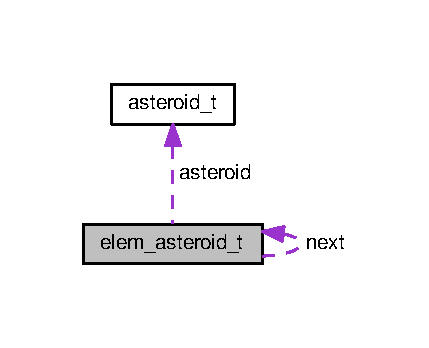
\includegraphics[width=206pt]{d3/d7b/structelem__asteroid__t__coll__graph}
\end{center}
\end{figure}
\subsection*{Attributi pubblici}
\begin{DoxyCompactItemize}
\item 
\hyperlink{structasteroid__t}{asteroid\+\_\+t} \hyperlink{structelem__asteroid__t_aada6a67a7d9b0d76f5bc73b82feb1e2a}{asteroid}
\item 
\hyperlink{structelem__asteroid__t}{elem\+\_\+asteroid\+\_\+t} $\ast$ \hyperlink{structelem__asteroid__t_a5f906717abd1758a220cbb1c1e5e1c9d}{next}
\end{DoxyCompactItemize}


\subsection{Descrizione dettagliata}
Struct del singolo elemento di una lista di asteroidi. 

~\newline
Campi\+: ~\newline
1) asteroid -\/ Asteroide; ~\newline
2) next -\/ Puntatore al prossimo elemento. 

\subsection{Documentazione dei membri dato}
\mbox{\Hypertarget{structelem__asteroid__t_aada6a67a7d9b0d76f5bc73b82feb1e2a}\label{structelem__asteroid__t_aada6a67a7d9b0d76f5bc73b82feb1e2a}} 
\index{elem\+\_\+asteroid\+\_\+t@{elem\+\_\+asteroid\+\_\+t}!asteroid@{asteroid}}
\index{asteroid@{asteroid}!elem\+\_\+asteroid\+\_\+t@{elem\+\_\+asteroid\+\_\+t}}
\subsubsection{\texorpdfstring{asteroid}{asteroid}}
{\footnotesize\ttfamily \hyperlink{structasteroid__t}{asteroid\+\_\+t} elem\+\_\+asteroid\+\_\+t\+::asteroid}

\mbox{\Hypertarget{structelem__asteroid__t_a5f906717abd1758a220cbb1c1e5e1c9d}\label{structelem__asteroid__t_a5f906717abd1758a220cbb1c1e5e1c9d}} 
\index{elem\+\_\+asteroid\+\_\+t@{elem\+\_\+asteroid\+\_\+t}!next@{next}}
\index{next@{next}!elem\+\_\+asteroid\+\_\+t@{elem\+\_\+asteroid\+\_\+t}}
\subsubsection{\texorpdfstring{next}{next}}
{\footnotesize\ttfamily \hyperlink{structelem__asteroid__t}{elem\+\_\+asteroid\+\_\+t}$\ast$ elem\+\_\+asteroid\+\_\+t\+::next}



La documentazione per questa struct è stata generata a partire dal seguente file\+:\begin{DoxyCompactItemize}
\item 
\hyperlink{data_8h}{data.\+h}\end{DoxyCompactItemize}

\hypertarget{structfile__t}{}\section{Riferimenti per la struct file\+\_\+t}
\label{structfile__t}\index{file\+\_\+t@{file\+\_\+t}}


Struct relativa alla descrizione di un archivio che andrà esaminato.  




{\ttfamily \#include $<$data.\+h$>$}

\subsection*{Attributi pubblici}
\begin{DoxyCompactItemize}
\item 
char $\ast$ \hyperlink{structfile__t_aead43b28cb333d0ee2beebe5f6cdfb41}{filename}
\item 
long int \hyperlink{structfile__t_a778e75e779fa9121918f668f4f452acf}{size}
\end{DoxyCompactItemize}


\subsection{Descrizione dettagliata}
Struct relativa alla descrizione di un archivio che andrà esaminato. 

~\newline
Raccoglie il nome (l\textquotesingle{}intero percorso) e la sua dimensione per poterli ordinare. 

\subsection{Documentazione dei membri dato}
\mbox{\Hypertarget{structfile__t_aead43b28cb333d0ee2beebe5f6cdfb41}\label{structfile__t_aead43b28cb333d0ee2beebe5f6cdfb41}} 
\index{file\+\_\+t@{file\+\_\+t}!filename@{filename}}
\index{filename@{filename}!file\+\_\+t@{file\+\_\+t}}
\subsubsection{\texorpdfstring{filename}{filename}}
{\footnotesize\ttfamily char$\ast$ file\+\_\+t\+::filename}

\mbox{\Hypertarget{structfile__t_a778e75e779fa9121918f668f4f452acf}\label{structfile__t_a778e75e779fa9121918f668f4f452acf}} 
\index{file\+\_\+t@{file\+\_\+t}!size@{size}}
\index{size@{size}!file\+\_\+t@{file\+\_\+t}}
\subsubsection{\texorpdfstring{size}{size}}
{\footnotesize\ttfamily long int file\+\_\+t\+::size}



La documentazione per questa struct è stata generata a partire dal seguente file\+:\begin{DoxyCompactItemize}
\item 
\hyperlink{data_8h}{data.\+h}\end{DoxyCompactItemize}

\hypertarget{structgeneral__gv__t}{}\section{Riferimenti per la struct general\+\_\+gv\+\_\+t}
\label{structgeneral__gv__t}\index{general\+\_\+gv\+\_\+t@{general\+\_\+gv\+\_\+t}}


Struct relativo alle proporzioni grafiche generali.  




{\ttfamily \#include $<$data.\+h$>$}

\subsection*{Attributi pubblici}
\begin{DoxyCompactItemize}
\item 
float \hyperlink{structgeneral__gv__t_a572bbf656ce2913288a07ce2d47c3fbe}{H\+E\+A\+D\+\_\+\+T\+O\+P\+\_\+\+O\+F\+F\+S\+ET}
\item 
float \hyperlink{structgeneral__gv__t_a99202d29316c566754e9602ef64a6875}{H\+E\+A\+D\+\_\+\+T\+E\+X\+T\+\_\+\+S\+H\+A\+D\+O\+W\+\_\+\+G\+AP}
\item 
float \hyperlink{structgeneral__gv__t_a6b15c19b5213f9cc0939caf7f7179086}{B\+A\+C\+K\+\_\+\+T\+O\+P\+\_\+\+O\+F\+F\+S\+ET}
\item 
float \hyperlink{structgeneral__gv__t_a977c6a75224caf8b71e8ce76f24a17e6}{B\+A\+C\+K\+\_\+\+L\+E\+F\+T\+\_\+\+O\+F\+F\+S\+ET}
\item 
float \hyperlink{structgeneral__gv__t_a7dcf5314af403550ee904c6fc3140703}{B\+A\+C\+K\+\_\+\+T\+E\+X\+T\+\_\+\+S\+H\+A\+D\+O\+W\+\_\+\+G\+AP}
\item 
float \hyperlink{structgeneral__gv__t_a95a0f12e648e993d277629fe2e83751e}{R\+E\+S\+U\+L\+T\+\_\+\+T\+O\+P\+\_\+\+O\+F\+F\+S\+ET}
\item 
int \hyperlink{structgeneral__gv__t_ad758522df3a3ddb6a6b6da8bc15be8aa}{H\+E\+A\+D\+\_\+\+F\+O\+N\+T\+S\+I\+ZE}
\item 
int \hyperlink{structgeneral__gv__t_a75427eccaa66bb0e209a080e5c50da66}{B\+A\+C\+K\+\_\+\+F\+O\+N\+T\+S\+I\+ZE}
\end{DoxyCompactItemize}


\subsection{Descrizione dettagliata}
Struct relativo alle proporzioni grafiche generali. 

\subsection{Documentazione dei membri dato}
\mbox{\Hypertarget{structgeneral__gv__t_a75427eccaa66bb0e209a080e5c50da66}\label{structgeneral__gv__t_a75427eccaa66bb0e209a080e5c50da66}} 
\index{general\+\_\+gv\+\_\+t@{general\+\_\+gv\+\_\+t}!B\+A\+C\+K\+\_\+\+F\+O\+N\+T\+S\+I\+ZE@{B\+A\+C\+K\+\_\+\+F\+O\+N\+T\+S\+I\+ZE}}
\index{B\+A\+C\+K\+\_\+\+F\+O\+N\+T\+S\+I\+ZE@{B\+A\+C\+K\+\_\+\+F\+O\+N\+T\+S\+I\+ZE}!general\+\_\+gv\+\_\+t@{general\+\_\+gv\+\_\+t}}
\subsubsection{\texorpdfstring{B\+A\+C\+K\+\_\+\+F\+O\+N\+T\+S\+I\+ZE}{BACK\_FONTSIZE}}
{\footnotesize\ttfamily int general\+\_\+gv\+\_\+t\+::\+B\+A\+C\+K\+\_\+\+F\+O\+N\+T\+S\+I\+ZE}

\mbox{\Hypertarget{structgeneral__gv__t_a977c6a75224caf8b71e8ce76f24a17e6}\label{structgeneral__gv__t_a977c6a75224caf8b71e8ce76f24a17e6}} 
\index{general\+\_\+gv\+\_\+t@{general\+\_\+gv\+\_\+t}!B\+A\+C\+K\+\_\+\+L\+E\+F\+T\+\_\+\+O\+F\+F\+S\+ET@{B\+A\+C\+K\+\_\+\+L\+E\+F\+T\+\_\+\+O\+F\+F\+S\+ET}}
\index{B\+A\+C\+K\+\_\+\+L\+E\+F\+T\+\_\+\+O\+F\+F\+S\+ET@{B\+A\+C\+K\+\_\+\+L\+E\+F\+T\+\_\+\+O\+F\+F\+S\+ET}!general\+\_\+gv\+\_\+t@{general\+\_\+gv\+\_\+t}}
\subsubsection{\texorpdfstring{B\+A\+C\+K\+\_\+\+L\+E\+F\+T\+\_\+\+O\+F\+F\+S\+ET}{BACK\_LEFT\_OFFSET}}
{\footnotesize\ttfamily float general\+\_\+gv\+\_\+t\+::\+B\+A\+C\+K\+\_\+\+L\+E\+F\+T\+\_\+\+O\+F\+F\+S\+ET}

\mbox{\Hypertarget{structgeneral__gv__t_a7dcf5314af403550ee904c6fc3140703}\label{structgeneral__gv__t_a7dcf5314af403550ee904c6fc3140703}} 
\index{general\+\_\+gv\+\_\+t@{general\+\_\+gv\+\_\+t}!B\+A\+C\+K\+\_\+\+T\+E\+X\+T\+\_\+\+S\+H\+A\+D\+O\+W\+\_\+\+G\+AP@{B\+A\+C\+K\+\_\+\+T\+E\+X\+T\+\_\+\+S\+H\+A\+D\+O\+W\+\_\+\+G\+AP}}
\index{B\+A\+C\+K\+\_\+\+T\+E\+X\+T\+\_\+\+S\+H\+A\+D\+O\+W\+\_\+\+G\+AP@{B\+A\+C\+K\+\_\+\+T\+E\+X\+T\+\_\+\+S\+H\+A\+D\+O\+W\+\_\+\+G\+AP}!general\+\_\+gv\+\_\+t@{general\+\_\+gv\+\_\+t}}
\subsubsection{\texorpdfstring{B\+A\+C\+K\+\_\+\+T\+E\+X\+T\+\_\+\+S\+H\+A\+D\+O\+W\+\_\+\+G\+AP}{BACK\_TEXT\_SHADOW\_GAP}}
{\footnotesize\ttfamily float general\+\_\+gv\+\_\+t\+::\+B\+A\+C\+K\+\_\+\+T\+E\+X\+T\+\_\+\+S\+H\+A\+D\+O\+W\+\_\+\+G\+AP}

\mbox{\Hypertarget{structgeneral__gv__t_a6b15c19b5213f9cc0939caf7f7179086}\label{structgeneral__gv__t_a6b15c19b5213f9cc0939caf7f7179086}} 
\index{general\+\_\+gv\+\_\+t@{general\+\_\+gv\+\_\+t}!B\+A\+C\+K\+\_\+\+T\+O\+P\+\_\+\+O\+F\+F\+S\+ET@{B\+A\+C\+K\+\_\+\+T\+O\+P\+\_\+\+O\+F\+F\+S\+ET}}
\index{B\+A\+C\+K\+\_\+\+T\+O\+P\+\_\+\+O\+F\+F\+S\+ET@{B\+A\+C\+K\+\_\+\+T\+O\+P\+\_\+\+O\+F\+F\+S\+ET}!general\+\_\+gv\+\_\+t@{general\+\_\+gv\+\_\+t}}
\subsubsection{\texorpdfstring{B\+A\+C\+K\+\_\+\+T\+O\+P\+\_\+\+O\+F\+F\+S\+ET}{BACK\_TOP\_OFFSET}}
{\footnotesize\ttfamily float general\+\_\+gv\+\_\+t\+::\+B\+A\+C\+K\+\_\+\+T\+O\+P\+\_\+\+O\+F\+F\+S\+ET}

\mbox{\Hypertarget{structgeneral__gv__t_ad758522df3a3ddb6a6b6da8bc15be8aa}\label{structgeneral__gv__t_ad758522df3a3ddb6a6b6da8bc15be8aa}} 
\index{general\+\_\+gv\+\_\+t@{general\+\_\+gv\+\_\+t}!H\+E\+A\+D\+\_\+\+F\+O\+N\+T\+S\+I\+ZE@{H\+E\+A\+D\+\_\+\+F\+O\+N\+T\+S\+I\+ZE}}
\index{H\+E\+A\+D\+\_\+\+F\+O\+N\+T\+S\+I\+ZE@{H\+E\+A\+D\+\_\+\+F\+O\+N\+T\+S\+I\+ZE}!general\+\_\+gv\+\_\+t@{general\+\_\+gv\+\_\+t}}
\subsubsection{\texorpdfstring{H\+E\+A\+D\+\_\+\+F\+O\+N\+T\+S\+I\+ZE}{HEAD\_FONTSIZE}}
{\footnotesize\ttfamily int general\+\_\+gv\+\_\+t\+::\+H\+E\+A\+D\+\_\+\+F\+O\+N\+T\+S\+I\+ZE}

\mbox{\Hypertarget{structgeneral__gv__t_a99202d29316c566754e9602ef64a6875}\label{structgeneral__gv__t_a99202d29316c566754e9602ef64a6875}} 
\index{general\+\_\+gv\+\_\+t@{general\+\_\+gv\+\_\+t}!H\+E\+A\+D\+\_\+\+T\+E\+X\+T\+\_\+\+S\+H\+A\+D\+O\+W\+\_\+\+G\+AP@{H\+E\+A\+D\+\_\+\+T\+E\+X\+T\+\_\+\+S\+H\+A\+D\+O\+W\+\_\+\+G\+AP}}
\index{H\+E\+A\+D\+\_\+\+T\+E\+X\+T\+\_\+\+S\+H\+A\+D\+O\+W\+\_\+\+G\+AP@{H\+E\+A\+D\+\_\+\+T\+E\+X\+T\+\_\+\+S\+H\+A\+D\+O\+W\+\_\+\+G\+AP}!general\+\_\+gv\+\_\+t@{general\+\_\+gv\+\_\+t}}
\subsubsection{\texorpdfstring{H\+E\+A\+D\+\_\+\+T\+E\+X\+T\+\_\+\+S\+H\+A\+D\+O\+W\+\_\+\+G\+AP}{HEAD\_TEXT\_SHADOW\_GAP}}
{\footnotesize\ttfamily float general\+\_\+gv\+\_\+t\+::\+H\+E\+A\+D\+\_\+\+T\+E\+X\+T\+\_\+\+S\+H\+A\+D\+O\+W\+\_\+\+G\+AP}

\mbox{\Hypertarget{structgeneral__gv__t_a572bbf656ce2913288a07ce2d47c3fbe}\label{structgeneral__gv__t_a572bbf656ce2913288a07ce2d47c3fbe}} 
\index{general\+\_\+gv\+\_\+t@{general\+\_\+gv\+\_\+t}!H\+E\+A\+D\+\_\+\+T\+O\+P\+\_\+\+O\+F\+F\+S\+ET@{H\+E\+A\+D\+\_\+\+T\+O\+P\+\_\+\+O\+F\+F\+S\+ET}}
\index{H\+E\+A\+D\+\_\+\+T\+O\+P\+\_\+\+O\+F\+F\+S\+ET@{H\+E\+A\+D\+\_\+\+T\+O\+P\+\_\+\+O\+F\+F\+S\+ET}!general\+\_\+gv\+\_\+t@{general\+\_\+gv\+\_\+t}}
\subsubsection{\texorpdfstring{H\+E\+A\+D\+\_\+\+T\+O\+P\+\_\+\+O\+F\+F\+S\+ET}{HEAD\_TOP\_OFFSET}}
{\footnotesize\ttfamily float general\+\_\+gv\+\_\+t\+::\+H\+E\+A\+D\+\_\+\+T\+O\+P\+\_\+\+O\+F\+F\+S\+ET}

\mbox{\Hypertarget{structgeneral__gv__t_a95a0f12e648e993d277629fe2e83751e}\label{structgeneral__gv__t_a95a0f12e648e993d277629fe2e83751e}} 
\index{general\+\_\+gv\+\_\+t@{general\+\_\+gv\+\_\+t}!R\+E\+S\+U\+L\+T\+\_\+\+T\+O\+P\+\_\+\+O\+F\+F\+S\+ET@{R\+E\+S\+U\+L\+T\+\_\+\+T\+O\+P\+\_\+\+O\+F\+F\+S\+ET}}
\index{R\+E\+S\+U\+L\+T\+\_\+\+T\+O\+P\+\_\+\+O\+F\+F\+S\+ET@{R\+E\+S\+U\+L\+T\+\_\+\+T\+O\+P\+\_\+\+O\+F\+F\+S\+ET}!general\+\_\+gv\+\_\+t@{general\+\_\+gv\+\_\+t}}
\subsubsection{\texorpdfstring{R\+E\+S\+U\+L\+T\+\_\+\+T\+O\+P\+\_\+\+O\+F\+F\+S\+ET}{RESULT\_TOP\_OFFSET}}
{\footnotesize\ttfamily float general\+\_\+gv\+\_\+t\+::\+R\+E\+S\+U\+L\+T\+\_\+\+T\+O\+P\+\_\+\+O\+F\+F\+S\+ET}



La documentazione per questa struct è stata generata a partire dal seguente file\+:\begin{DoxyCompactItemize}
\item 
\hyperlink{data_8h}{data.\+h}\end{DoxyCompactItemize}

\hypertarget{structinstr__gv__t}{}\section{Riferimenti per la struct instr\+\_\+gv\+\_\+t}
\label{structinstr__gv__t}\index{instr\+\_\+gv\+\_\+t@{instr\+\_\+gv\+\_\+t}}


Struct relativo alle proporzioni grafiche della schermata di pausa.  




{\ttfamily \#include $<$data.\+h$>$}

\subsection*{Attributi pubblici}
\begin{DoxyCompactItemize}
\item 
float \hyperlink{structinstr__gv__t_aadedcf5c3f9a7db3eb3214dc3aa961f7}{B\+O\+N\+U\+S\+\_\+\+R\+A\+D\+I\+US}
\item 
float \hyperlink{structinstr__gv__t_a7a92d03fee7f41bdbd681bb8342a35f8}{B\+O\+N\+U\+S\+\_\+\+C\+A\+S\+E\+\_\+\+W\+I\+D\+TH}
\item 
int \hyperlink{structinstr__gv__t_a552dc4715b763b4b5188d36ac2a06794}{S\+U\+B\+T\+I\+T\+L\+E\+\_\+\+F\+O\+N\+T\+S\+I\+ZE}
\item 
int \hyperlink{structinstr__gv__t_a44f052a2fd3ef87d6974c592945fdbaa}{T\+E\+X\+T\+\_\+\+F\+O\+N\+T\+S\+I\+ZE}
\end{DoxyCompactItemize}


\subsection{Descrizione dettagliata}
Struct relativo alle proporzioni grafiche della schermata di pausa. 

\subsection{Documentazione dei membri dato}
\mbox{\Hypertarget{structinstr__gv__t_a7a92d03fee7f41bdbd681bb8342a35f8}\label{structinstr__gv__t_a7a92d03fee7f41bdbd681bb8342a35f8}} 
\index{instr\+\_\+gv\+\_\+t@{instr\+\_\+gv\+\_\+t}!B\+O\+N\+U\+S\+\_\+\+C\+A\+S\+E\+\_\+\+W\+I\+D\+TH@{B\+O\+N\+U\+S\+\_\+\+C\+A\+S\+E\+\_\+\+W\+I\+D\+TH}}
\index{B\+O\+N\+U\+S\+\_\+\+C\+A\+S\+E\+\_\+\+W\+I\+D\+TH@{B\+O\+N\+U\+S\+\_\+\+C\+A\+S\+E\+\_\+\+W\+I\+D\+TH}!instr\+\_\+gv\+\_\+t@{instr\+\_\+gv\+\_\+t}}
\subsubsection{\texorpdfstring{B\+O\+N\+U\+S\+\_\+\+C\+A\+S\+E\+\_\+\+W\+I\+D\+TH}{BONUS\_CASE\_WIDTH}}
{\footnotesize\ttfamily float instr\+\_\+gv\+\_\+t\+::\+B\+O\+N\+U\+S\+\_\+\+C\+A\+S\+E\+\_\+\+W\+I\+D\+TH}

\mbox{\Hypertarget{structinstr__gv__t_aadedcf5c3f9a7db3eb3214dc3aa961f7}\label{structinstr__gv__t_aadedcf5c3f9a7db3eb3214dc3aa961f7}} 
\index{instr\+\_\+gv\+\_\+t@{instr\+\_\+gv\+\_\+t}!B\+O\+N\+U\+S\+\_\+\+R\+A\+D\+I\+US@{B\+O\+N\+U\+S\+\_\+\+R\+A\+D\+I\+US}}
\index{B\+O\+N\+U\+S\+\_\+\+R\+A\+D\+I\+US@{B\+O\+N\+U\+S\+\_\+\+R\+A\+D\+I\+US}!instr\+\_\+gv\+\_\+t@{instr\+\_\+gv\+\_\+t}}
\subsubsection{\texorpdfstring{B\+O\+N\+U\+S\+\_\+\+R\+A\+D\+I\+US}{BONUS\_RADIUS}}
{\footnotesize\ttfamily float instr\+\_\+gv\+\_\+t\+::\+B\+O\+N\+U\+S\+\_\+\+R\+A\+D\+I\+US}

\mbox{\Hypertarget{structinstr__gv__t_a552dc4715b763b4b5188d36ac2a06794}\label{structinstr__gv__t_a552dc4715b763b4b5188d36ac2a06794}} 
\index{instr\+\_\+gv\+\_\+t@{instr\+\_\+gv\+\_\+t}!S\+U\+B\+T\+I\+T\+L\+E\+\_\+\+F\+O\+N\+T\+S\+I\+ZE@{S\+U\+B\+T\+I\+T\+L\+E\+\_\+\+F\+O\+N\+T\+S\+I\+ZE}}
\index{S\+U\+B\+T\+I\+T\+L\+E\+\_\+\+F\+O\+N\+T\+S\+I\+ZE@{S\+U\+B\+T\+I\+T\+L\+E\+\_\+\+F\+O\+N\+T\+S\+I\+ZE}!instr\+\_\+gv\+\_\+t@{instr\+\_\+gv\+\_\+t}}
\subsubsection{\texorpdfstring{S\+U\+B\+T\+I\+T\+L\+E\+\_\+\+F\+O\+N\+T\+S\+I\+ZE}{SUBTITLE\_FONTSIZE}}
{\footnotesize\ttfamily int instr\+\_\+gv\+\_\+t\+::\+S\+U\+B\+T\+I\+T\+L\+E\+\_\+\+F\+O\+N\+T\+S\+I\+ZE}

\mbox{\Hypertarget{structinstr__gv__t_a44f052a2fd3ef87d6974c592945fdbaa}\label{structinstr__gv__t_a44f052a2fd3ef87d6974c592945fdbaa}} 
\index{instr\+\_\+gv\+\_\+t@{instr\+\_\+gv\+\_\+t}!T\+E\+X\+T\+\_\+\+F\+O\+N\+T\+S\+I\+ZE@{T\+E\+X\+T\+\_\+\+F\+O\+N\+T\+S\+I\+ZE}}
\index{T\+E\+X\+T\+\_\+\+F\+O\+N\+T\+S\+I\+ZE@{T\+E\+X\+T\+\_\+\+F\+O\+N\+T\+S\+I\+ZE}!instr\+\_\+gv\+\_\+t@{instr\+\_\+gv\+\_\+t}}
\subsubsection{\texorpdfstring{T\+E\+X\+T\+\_\+\+F\+O\+N\+T\+S\+I\+ZE}{TEXT\_FONTSIZE}}
{\footnotesize\ttfamily int instr\+\_\+gv\+\_\+t\+::\+T\+E\+X\+T\+\_\+\+F\+O\+N\+T\+S\+I\+ZE}



La documentazione per questa struct è stata generata a partire dal seguente file\+:\begin{DoxyCompactItemize}
\item 
\hyperlink{data_8h}{data.\+h}\end{DoxyCompactItemize}

\hypertarget{structlook__into__t}{}\section{Riferimenti per la struct look\+\_\+into\+\_\+t}
\label{structlook__into__t}\index{look\+\_\+into\+\_\+t@{look\+\_\+into\+\_\+t}}


Struct di appoggio utilizzata dai thread searcher/worker per ricevere informazioni riguardo\+: 1) filename -\/ dentro quale archivio cercare; 2) email -\/ quale email cercare; 3) is\+\_\+searcher -\/ se il thread si tratta di un searcher (fornisce le parole al gioco) o di un worker.  




{\ttfamily \#include $<$data.\+h$>$}

\subsection*{Attributi pubblici}
\begin{DoxyCompactItemize}
\item 
char $\ast$ \hyperlink{structlook__into__t_aac2e0d99d8a29764003eb408fe9a0992}{filename}
\item 
char $\ast$ \hyperlink{structlook__into__t_a0e9aa8914a44800cef56c29c296d9ba1}{email}
\item 
bool \hyperlink{structlook__into__t_a4f74ba613ccae77bdec049edb078e8c0}{is\+\_\+searcher}
\end{DoxyCompactItemize}


\subsection{Descrizione dettagliata}
Struct di appoggio utilizzata dai thread searcher/worker per ricevere informazioni riguardo\+: 1) filename -\/ dentro quale archivio cercare; 2) email -\/ quale email cercare; 3) is\+\_\+searcher -\/ se il thread si tratta di un searcher (fornisce le parole al gioco) o di un worker. 

\subsection{Documentazione dei membri dato}
\mbox{\Hypertarget{structlook__into__t_a0e9aa8914a44800cef56c29c296d9ba1}\label{structlook__into__t_a0e9aa8914a44800cef56c29c296d9ba1}} 
\index{look\+\_\+into\+\_\+t@{look\+\_\+into\+\_\+t}!email@{email}}
\index{email@{email}!look\+\_\+into\+\_\+t@{look\+\_\+into\+\_\+t}}
\subsubsection{\texorpdfstring{email}{email}}
{\footnotesize\ttfamily char$\ast$ look\+\_\+into\+\_\+t\+::email}

\mbox{\Hypertarget{structlook__into__t_aac2e0d99d8a29764003eb408fe9a0992}\label{structlook__into__t_aac2e0d99d8a29764003eb408fe9a0992}} 
\index{look\+\_\+into\+\_\+t@{look\+\_\+into\+\_\+t}!filename@{filename}}
\index{filename@{filename}!look\+\_\+into\+\_\+t@{look\+\_\+into\+\_\+t}}
\subsubsection{\texorpdfstring{filename}{filename}}
{\footnotesize\ttfamily char$\ast$ look\+\_\+into\+\_\+t\+::filename}

\mbox{\Hypertarget{structlook__into__t_a4f74ba613ccae77bdec049edb078e8c0}\label{structlook__into__t_a4f74ba613ccae77bdec049edb078e8c0}} 
\index{look\+\_\+into\+\_\+t@{look\+\_\+into\+\_\+t}!is\+\_\+searcher@{is\+\_\+searcher}}
\index{is\+\_\+searcher@{is\+\_\+searcher}!look\+\_\+into\+\_\+t@{look\+\_\+into\+\_\+t}}
\subsubsection{\texorpdfstring{is\+\_\+searcher}{is\_searcher}}
{\footnotesize\ttfamily bool look\+\_\+into\+\_\+t\+::is\+\_\+searcher}



La documentazione per questa struct è stata generata a partire dal seguente file\+:\begin{DoxyCompactItemize}
\item 
\hyperlink{data_8h}{data.\+h}\end{DoxyCompactItemize}

\hypertarget{structls__t}{}\section{Riferimenti per la struct ls\+\_\+t}
\label{structls__t}\index{ls\+\_\+t@{ls\+\_\+t}}


Struct che raccoglie tutti gli archivi.  




{\ttfamily \#include $<$data.\+h$>$}



Diagramma di collaborazione per ls\+\_\+t\+:\nopagebreak
\begin{figure}[H]
\begin{center}
\leavevmode
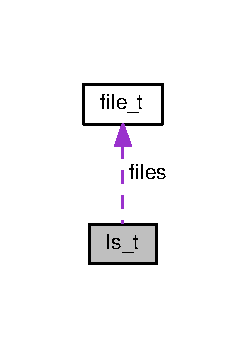
\includegraphics[width=121pt]{d7/d32/structls__t__coll__graph}
\end{center}
\end{figure}
\subsection*{Attributi pubblici}
\begin{DoxyCompactItemize}
\item 
\hyperlink{structfile__t}{file\+\_\+t} $\ast$ \hyperlink{structls__t_af312bfe211803fb5171b556d1e9ee82a}{files}
\item 
int \hyperlink{structls__t_abb4496e90c61f2a5af018644b8a7441e}{nfile}
\end{DoxyCompactItemize}


\subsection{Descrizione dettagliata}
Struct che raccoglie tutti gli archivi. 

~\newline
Tiene anche conto di quelli letti attraverso un array di flag. 

\subsection{Documentazione dei membri dato}
\mbox{\Hypertarget{structls__t_af312bfe211803fb5171b556d1e9ee82a}\label{structls__t_af312bfe211803fb5171b556d1e9ee82a}} 
\index{ls\+\_\+t@{ls\+\_\+t}!files@{files}}
\index{files@{files}!ls\+\_\+t@{ls\+\_\+t}}
\subsubsection{\texorpdfstring{files}{files}}
{\footnotesize\ttfamily \hyperlink{structfile__t}{file\+\_\+t}$\ast$ ls\+\_\+t\+::files}

\mbox{\Hypertarget{structls__t_abb4496e90c61f2a5af018644b8a7441e}\label{structls__t_abb4496e90c61f2a5af018644b8a7441e}} 
\index{ls\+\_\+t@{ls\+\_\+t}!nfile@{nfile}}
\index{nfile@{nfile}!ls\+\_\+t@{ls\+\_\+t}}
\subsubsection{\texorpdfstring{nfile}{nfile}}
{\footnotesize\ttfamily int ls\+\_\+t\+::nfile}



La documentazione per questa struct è stata generata a partire dal seguente file\+:\begin{DoxyCompactItemize}
\item 
\hyperlink{data_8h}{data.\+h}\end{DoxyCompactItemize}

\hypertarget{structmatch__vars__t}{}\section{Riferimenti per la struct match\+\_\+vars\+\_\+t}
\label{structmatch__vars__t}\index{match\+\_\+vars\+\_\+t@{match\+\_\+vars\+\_\+t}}


Struct contenente le variabili di gioco.  




{\ttfamily \#include $<$data.\+h$>$}



Diagramma di collaborazione per match\+\_\+vars\+\_\+t\+:\nopagebreak
\begin{figure}[H]
\begin{center}
\leavevmode
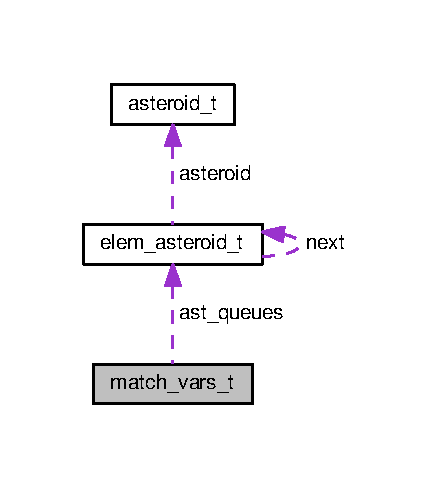
\includegraphics[width=206pt]{d2/db7/structmatch__vars__t__coll__graph}
\end{center}
\end{figure}
\subsection*{Attributi pubblici}
\begin{DoxyCompactItemize}
\item 
\hyperlink{data_8h_a452eef9acfcf76fb85e2c7ecf3b9ff90}{asteroid\+\_\+list} \hyperlink{structmatch__vars__t_a71ec4212320d46caf051a7e61addbffe}{ast\+\_\+queues} \mbox{[}\hyperlink{data_8h_abbb1a97343fdbf54e75f14fb83cb0a92}{N\+\_\+\+Q\+U\+E\+U\+ES}\mbox{]}
\item 
int \hyperlink{structmatch__vars__t_aa002d177fd16ff93c89394a68fd469a0}{score}
\item 
int \hyperlink{structmatch__vars__t_ab2a6e3340cca84e388bae6a0bc3e0425}{asteroids\+\_\+destroyed}
\item 
A\+L\+L\+E\+G\+R\+O\+\_\+\+T\+I\+M\+ER $\ast$ \hyperlink{structmatch__vars__t_a3f2d3e6df0eba86392ef88491d1e31bd}{spawn\+\_\+timer}
\item 
double \hyperlink{structmatch__vars__t_a82b9a455eeeb8653c724fb6ab555ab01}{spawn\+\_\+interval}
\item 
A\+L\+L\+E\+G\+R\+O\+\_\+\+T\+I\+M\+ER $\ast$ \hyperlink{structmatch__vars__t_a98409cabd79c20cd80959cb2242e683c}{timer\+\_\+shield\+\_\+bonus}
\item 
A\+L\+L\+E\+G\+R\+O\+\_\+\+T\+I\+M\+ER $\ast$ \hyperlink{structmatch__vars__t_a943d3f8a5a80e3840b4c034893ad3d72}{timer\+\_\+rallenty\+\_\+bonus}
\item 
float \hyperlink{structmatch__vars__t_a1b8a66b48d6fb51e5bcdfd6c66da1102}{fps}
\item 
int \hyperlink{structmatch__vars__t_a8b93e95f0caf4fa72707e6e234446751}{insert\+\_\+asteroid\+\_\+index}
\item 
int \hyperlink{structmatch__vars__t_a19eb567824590a0ae36be4ed146c1a89}{asteroid\+\_\+head}
\item 
\hyperlink{data_8h_a07b940e2e86eb4fc3f1e1e1843da0564}{asteroid\+\_\+special\+\_\+t} \hyperlink{structmatch__vars__t_a776555bc52d4be60612230e4735fe467}{asteroid\+\_\+to\+\_\+generate}
\item 
A\+L\+L\+E\+G\+R\+O\+\_\+\+S\+A\+M\+P\+LE $\ast$ \hyperlink{structmatch__vars__t_aefc460782c12de4ae0c1fdbd9f7c531d}{sound\+\_\+exp}
\item 
A\+L\+L\+E\+G\+R\+O\+\_\+\+S\+A\+M\+P\+LE $\ast$ \hyperlink{structmatch__vars__t_ac379900bede23a881327a9951a020dc6}{sound\+\_\+fire}
\item 
A\+L\+L\+E\+G\+R\+O\+\_\+\+S\+A\+M\+P\+LE $\ast$ \hyperlink{structmatch__vars__t_a31831089835f2f553993d69e4c0c3d1b}{sound\+\_\+gameover}
\item 
A\+L\+L\+E\+G\+R\+O\+\_\+\+S\+A\+M\+P\+LE $\ast$ \hyperlink{structmatch__vars__t_a76f812bd8ea550d3e61ebfa185c3471a}{sound\+\_\+error}
\item 
A\+L\+L\+E\+G\+R\+O\+\_\+\+S\+A\+M\+P\+L\+E\+\_\+\+I\+N\+S\+T\+A\+N\+CE $\ast$ \hyperlink{structmatch__vars__t_a1565ecf6c28c18912372ef685ec9627f}{music\+\_\+playwa}
\item 
int \hyperlink{structmatch__vars__t_aec99582de5c65954b0cf568f1d702427}{current\+\_\+asteroid}
\item 
int \hyperlink{structmatch__vars__t_ab682954df4b3c57c0808d1f0975134ae}{key\+\_\+error}
\item 
\hyperlink{data_8h_a56839c56ca6deb3cff5e21540ddb8218}{enable\+\_\+t} \hyperlink{structmatch__vars__t_a726fe4ae3e07b478c2753115e71030f0}{playing}
\item 
bool \hyperlink{structmatch__vars__t_a2d403d1bd9faac481e4508b771b8ba69}{gameover}
\item 
int \hyperlink{structmatch__vars__t_a888b72765ff70c20f1d7980a00f3603c}{items} \mbox{[}\hyperlink{data_8h_affced4b175e803df59f802e25d017b9b}{N\+U\+M\+\_\+\+I\+T\+E\+MS}\mbox{]}
\item 
int \hyperlink{structmatch__vars__t_a2775d451ad359f3296dbfa36da5cca82}{asteroid\+\_\+to\+\_\+bonus}
\item 
int \hyperlink{structmatch__vars__t_a6d48827959334e36fca668b19fe1fe77}{instant\+\_\+ast\+\_\+dest}
\end{DoxyCompactItemize}


\subsection{Descrizione dettagliata}
Struct contenente le variabili di gioco. 

~\newline
Campi\+: ~\newline
1) ast\+\_\+queues -\/ Array di liste di asteroidi; ~\newline
2) score -\/ Punteggio; ~\newline
3) asteroids\+\_\+destroyed -\/ Numero di asteroidi distrutti; ~\newline
4) spawn\+\_\+interval -\/ Tempo di attesa (espresso in secondi) tra la generazione di due asteroidi; ~\newline
5) spawn\+\_\+timer -\/ Timer relativo alla generazione di asteroidi; ~\newline
6) timer\+\_\+shield\+\_\+bonus -\/ Timer relativo alla durata del bonus \char`\"{}\+Shield\char`\"{}; ~\newline
7) timer\+\_\+rallenty\+\_\+bonus -\/ Timer relativo alla durata del bonus \char`\"{}\+Rallenty\char`\"{}; ~\newline
8) fps -\/ Intervallo di refresh della schermata; ~\newline
9) diff\+\_\+liv -\/ Livello di difficoltà del gioco (\mbox{[}3,14\mbox{]}); ~\newline
10) insert\+\_\+asteroid\+\_\+index -\/ Indice che dice se c\textquotesingle{}è un asteroide in coda che andrà fatto comparire nel gioco; ~\newline
11) asteroid\+\_\+head -\/ Numero di asteroidi presenti in testa nel vettore delle liste (\mbox{[}0,N\+U\+M\+\_\+\+Q\+U\+E\+U\+ES\mbox{]}); ~\newline
12) asteroid\+\_\+to\+\_\+generate -\/ Tipo dell\textquotesingle{}asteroide che verrà generato; ~\newline
 ~\newline
13) sound\+\_\+exp -\/ Suono dell\textquotesingle{}esplosione di un asteroide; ~\newline
14) sound\+\_\+fire -\/ Suono dello sparo di un proiettile; ~\newline
15) sound\+\_\+gameover -\/ Suono che viene eseguito quando si verifica il gameover; ~\newline
16) sound\+\_\+rallenty -\/ Suono che sostituisce la musica durante il bonus \char`\"{}\+Rallenty\char`\"{}; ~\newline
17) sound\+\_\+error -\/ Suono che viene eseguito quando si digita una lettera sbagliata; ~\newline
18) current\+\_\+asteroid -\/ Indice dell\textquotesingle{}asteroide che si sta cercando di distruggere. ~\newline
 Vale -\/1 se si deve ancora agganciare un asteroide da colipire; ~\newline
19) key\+\_\+error -\/ Indice dell\textquotesingle{}asteroide del quale si è sbagliata la lettera. Vale -\/1 se non vi sono errori; ~\newline
20) playing -\/ Variabile che indica se il gioco è in pausa o si sta giocando; ~\newline
21) gameover -\/ Variabile che indica se si è verificato il gameover; ~\newline
 ~\newline
22) items -\/ Array dei bonus\+: indica la numerosità di ognuno dei quattro bonus; ~\newline
23) asteroid\+\_\+to\+\_\+bonus -\/ Numero di asteroidi da distruggere per ottenere un bonus; ~\newline
24) instant\+\_\+ast\+\_\+dest -\/ Numero di asteroidi distrutti in un determinato istante, in modo da calcolare se si è arrivati al bonus. 

\subsection{Documentazione dei membri dato}
\mbox{\Hypertarget{structmatch__vars__t_a71ec4212320d46caf051a7e61addbffe}\label{structmatch__vars__t_a71ec4212320d46caf051a7e61addbffe}} 
\index{match\+\_\+vars\+\_\+t@{match\+\_\+vars\+\_\+t}!ast\+\_\+queues@{ast\+\_\+queues}}
\index{ast\+\_\+queues@{ast\+\_\+queues}!match\+\_\+vars\+\_\+t@{match\+\_\+vars\+\_\+t}}
\subsubsection{\texorpdfstring{ast\+\_\+queues}{ast\_queues}}
{\footnotesize\ttfamily \hyperlink{data_8h_a452eef9acfcf76fb85e2c7ecf3b9ff90}{asteroid\+\_\+list} match\+\_\+vars\+\_\+t\+::ast\+\_\+queues\mbox{[}\hyperlink{data_8h_abbb1a97343fdbf54e75f14fb83cb0a92}{N\+\_\+\+Q\+U\+E\+U\+ES}\mbox{]}}

\mbox{\Hypertarget{structmatch__vars__t_a19eb567824590a0ae36be4ed146c1a89}\label{structmatch__vars__t_a19eb567824590a0ae36be4ed146c1a89}} 
\index{match\+\_\+vars\+\_\+t@{match\+\_\+vars\+\_\+t}!asteroid\+\_\+head@{asteroid\+\_\+head}}
\index{asteroid\+\_\+head@{asteroid\+\_\+head}!match\+\_\+vars\+\_\+t@{match\+\_\+vars\+\_\+t}}
\subsubsection{\texorpdfstring{asteroid\+\_\+head}{asteroid\_head}}
{\footnotesize\ttfamily int match\+\_\+vars\+\_\+t\+::asteroid\+\_\+head}

\mbox{\Hypertarget{structmatch__vars__t_a2775d451ad359f3296dbfa36da5cca82}\label{structmatch__vars__t_a2775d451ad359f3296dbfa36da5cca82}} 
\index{match\+\_\+vars\+\_\+t@{match\+\_\+vars\+\_\+t}!asteroid\+\_\+to\+\_\+bonus@{asteroid\+\_\+to\+\_\+bonus}}
\index{asteroid\+\_\+to\+\_\+bonus@{asteroid\+\_\+to\+\_\+bonus}!match\+\_\+vars\+\_\+t@{match\+\_\+vars\+\_\+t}}
\subsubsection{\texorpdfstring{asteroid\+\_\+to\+\_\+bonus}{asteroid\_to\_bonus}}
{\footnotesize\ttfamily int match\+\_\+vars\+\_\+t\+::asteroid\+\_\+to\+\_\+bonus}

\mbox{\Hypertarget{structmatch__vars__t_a776555bc52d4be60612230e4735fe467}\label{structmatch__vars__t_a776555bc52d4be60612230e4735fe467}} 
\index{match\+\_\+vars\+\_\+t@{match\+\_\+vars\+\_\+t}!asteroid\+\_\+to\+\_\+generate@{asteroid\+\_\+to\+\_\+generate}}
\index{asteroid\+\_\+to\+\_\+generate@{asteroid\+\_\+to\+\_\+generate}!match\+\_\+vars\+\_\+t@{match\+\_\+vars\+\_\+t}}
\subsubsection{\texorpdfstring{asteroid\+\_\+to\+\_\+generate}{asteroid\_to\_generate}}
{\footnotesize\ttfamily \hyperlink{data_8h_a07b940e2e86eb4fc3f1e1e1843da0564}{asteroid\+\_\+special\+\_\+t} match\+\_\+vars\+\_\+t\+::asteroid\+\_\+to\+\_\+generate}

\mbox{\Hypertarget{structmatch__vars__t_ab2a6e3340cca84e388bae6a0bc3e0425}\label{structmatch__vars__t_ab2a6e3340cca84e388bae6a0bc3e0425}} 
\index{match\+\_\+vars\+\_\+t@{match\+\_\+vars\+\_\+t}!asteroids\+\_\+destroyed@{asteroids\+\_\+destroyed}}
\index{asteroids\+\_\+destroyed@{asteroids\+\_\+destroyed}!match\+\_\+vars\+\_\+t@{match\+\_\+vars\+\_\+t}}
\subsubsection{\texorpdfstring{asteroids\+\_\+destroyed}{asteroids\_destroyed}}
{\footnotesize\ttfamily int match\+\_\+vars\+\_\+t\+::asteroids\+\_\+destroyed}

\mbox{\Hypertarget{structmatch__vars__t_aec99582de5c65954b0cf568f1d702427}\label{structmatch__vars__t_aec99582de5c65954b0cf568f1d702427}} 
\index{match\+\_\+vars\+\_\+t@{match\+\_\+vars\+\_\+t}!current\+\_\+asteroid@{current\+\_\+asteroid}}
\index{current\+\_\+asteroid@{current\+\_\+asteroid}!match\+\_\+vars\+\_\+t@{match\+\_\+vars\+\_\+t}}
\subsubsection{\texorpdfstring{current\+\_\+asteroid}{current\_asteroid}}
{\footnotesize\ttfamily int match\+\_\+vars\+\_\+t\+::current\+\_\+asteroid}

\mbox{\Hypertarget{structmatch__vars__t_a1b8a66b48d6fb51e5bcdfd6c66da1102}\label{structmatch__vars__t_a1b8a66b48d6fb51e5bcdfd6c66da1102}} 
\index{match\+\_\+vars\+\_\+t@{match\+\_\+vars\+\_\+t}!fps@{fps}}
\index{fps@{fps}!match\+\_\+vars\+\_\+t@{match\+\_\+vars\+\_\+t}}
\subsubsection{\texorpdfstring{fps}{fps}}
{\footnotesize\ttfamily float match\+\_\+vars\+\_\+t\+::fps}

\mbox{\Hypertarget{structmatch__vars__t_a2d403d1bd9faac481e4508b771b8ba69}\label{structmatch__vars__t_a2d403d1bd9faac481e4508b771b8ba69}} 
\index{match\+\_\+vars\+\_\+t@{match\+\_\+vars\+\_\+t}!gameover@{gameover}}
\index{gameover@{gameover}!match\+\_\+vars\+\_\+t@{match\+\_\+vars\+\_\+t}}
\subsubsection{\texorpdfstring{gameover}{gameover}}
{\footnotesize\ttfamily bool match\+\_\+vars\+\_\+t\+::gameover}

\mbox{\Hypertarget{structmatch__vars__t_a8b93e95f0caf4fa72707e6e234446751}\label{structmatch__vars__t_a8b93e95f0caf4fa72707e6e234446751}} 
\index{match\+\_\+vars\+\_\+t@{match\+\_\+vars\+\_\+t}!insert\+\_\+asteroid\+\_\+index@{insert\+\_\+asteroid\+\_\+index}}
\index{insert\+\_\+asteroid\+\_\+index@{insert\+\_\+asteroid\+\_\+index}!match\+\_\+vars\+\_\+t@{match\+\_\+vars\+\_\+t}}
\subsubsection{\texorpdfstring{insert\+\_\+asteroid\+\_\+index}{insert\_asteroid\_index}}
{\footnotesize\ttfamily int match\+\_\+vars\+\_\+t\+::insert\+\_\+asteroid\+\_\+index}

\mbox{\Hypertarget{structmatch__vars__t_a6d48827959334e36fca668b19fe1fe77}\label{structmatch__vars__t_a6d48827959334e36fca668b19fe1fe77}} 
\index{match\+\_\+vars\+\_\+t@{match\+\_\+vars\+\_\+t}!instant\+\_\+ast\+\_\+dest@{instant\+\_\+ast\+\_\+dest}}
\index{instant\+\_\+ast\+\_\+dest@{instant\+\_\+ast\+\_\+dest}!match\+\_\+vars\+\_\+t@{match\+\_\+vars\+\_\+t}}
\subsubsection{\texorpdfstring{instant\+\_\+ast\+\_\+dest}{instant\_ast\_dest}}
{\footnotesize\ttfamily int match\+\_\+vars\+\_\+t\+::instant\+\_\+ast\+\_\+dest}

\mbox{\Hypertarget{structmatch__vars__t_a888b72765ff70c20f1d7980a00f3603c}\label{structmatch__vars__t_a888b72765ff70c20f1d7980a00f3603c}} 
\index{match\+\_\+vars\+\_\+t@{match\+\_\+vars\+\_\+t}!items@{items}}
\index{items@{items}!match\+\_\+vars\+\_\+t@{match\+\_\+vars\+\_\+t}}
\subsubsection{\texorpdfstring{items}{items}}
{\footnotesize\ttfamily int match\+\_\+vars\+\_\+t\+::items\mbox{[}\hyperlink{data_8h_affced4b175e803df59f802e25d017b9b}{N\+U\+M\+\_\+\+I\+T\+E\+MS}\mbox{]}}

\mbox{\Hypertarget{structmatch__vars__t_ab682954df4b3c57c0808d1f0975134ae}\label{structmatch__vars__t_ab682954df4b3c57c0808d1f0975134ae}} 
\index{match\+\_\+vars\+\_\+t@{match\+\_\+vars\+\_\+t}!key\+\_\+error@{key\+\_\+error}}
\index{key\+\_\+error@{key\+\_\+error}!match\+\_\+vars\+\_\+t@{match\+\_\+vars\+\_\+t}}
\subsubsection{\texorpdfstring{key\+\_\+error}{key\_error}}
{\footnotesize\ttfamily int match\+\_\+vars\+\_\+t\+::key\+\_\+error}

\mbox{\Hypertarget{structmatch__vars__t_a1565ecf6c28c18912372ef685ec9627f}\label{structmatch__vars__t_a1565ecf6c28c18912372ef685ec9627f}} 
\index{match\+\_\+vars\+\_\+t@{match\+\_\+vars\+\_\+t}!music\+\_\+playwa@{music\+\_\+playwa}}
\index{music\+\_\+playwa@{music\+\_\+playwa}!match\+\_\+vars\+\_\+t@{match\+\_\+vars\+\_\+t}}
\subsubsection{\texorpdfstring{music\+\_\+playwa}{music\_playwa}}
{\footnotesize\ttfamily A\+L\+L\+E\+G\+R\+O\+\_\+\+S\+A\+M\+P\+L\+E\+\_\+\+I\+N\+S\+T\+A\+N\+CE$\ast$ match\+\_\+vars\+\_\+t\+::music\+\_\+playwa}

\mbox{\Hypertarget{structmatch__vars__t_a726fe4ae3e07b478c2753115e71030f0}\label{structmatch__vars__t_a726fe4ae3e07b478c2753115e71030f0}} 
\index{match\+\_\+vars\+\_\+t@{match\+\_\+vars\+\_\+t}!playing@{playing}}
\index{playing@{playing}!match\+\_\+vars\+\_\+t@{match\+\_\+vars\+\_\+t}}
\subsubsection{\texorpdfstring{playing}{playing}}
{\footnotesize\ttfamily \hyperlink{data_8h_a56839c56ca6deb3cff5e21540ddb8218}{enable\+\_\+t} match\+\_\+vars\+\_\+t\+::playing}

\mbox{\Hypertarget{structmatch__vars__t_aa002d177fd16ff93c89394a68fd469a0}\label{structmatch__vars__t_aa002d177fd16ff93c89394a68fd469a0}} 
\index{match\+\_\+vars\+\_\+t@{match\+\_\+vars\+\_\+t}!score@{score}}
\index{score@{score}!match\+\_\+vars\+\_\+t@{match\+\_\+vars\+\_\+t}}
\subsubsection{\texorpdfstring{score}{score}}
{\footnotesize\ttfamily int match\+\_\+vars\+\_\+t\+::score}

\mbox{\Hypertarget{structmatch__vars__t_a76f812bd8ea550d3e61ebfa185c3471a}\label{structmatch__vars__t_a76f812bd8ea550d3e61ebfa185c3471a}} 
\index{match\+\_\+vars\+\_\+t@{match\+\_\+vars\+\_\+t}!sound\+\_\+error@{sound\+\_\+error}}
\index{sound\+\_\+error@{sound\+\_\+error}!match\+\_\+vars\+\_\+t@{match\+\_\+vars\+\_\+t}}
\subsubsection{\texorpdfstring{sound\+\_\+error}{sound\_error}}
{\footnotesize\ttfamily A\+L\+L\+E\+G\+R\+O\+\_\+\+S\+A\+M\+P\+LE$\ast$ match\+\_\+vars\+\_\+t\+::sound\+\_\+error}

\mbox{\Hypertarget{structmatch__vars__t_aefc460782c12de4ae0c1fdbd9f7c531d}\label{structmatch__vars__t_aefc460782c12de4ae0c1fdbd9f7c531d}} 
\index{match\+\_\+vars\+\_\+t@{match\+\_\+vars\+\_\+t}!sound\+\_\+exp@{sound\+\_\+exp}}
\index{sound\+\_\+exp@{sound\+\_\+exp}!match\+\_\+vars\+\_\+t@{match\+\_\+vars\+\_\+t}}
\subsubsection{\texorpdfstring{sound\+\_\+exp}{sound\_exp}}
{\footnotesize\ttfamily A\+L\+L\+E\+G\+R\+O\+\_\+\+S\+A\+M\+P\+LE$\ast$ match\+\_\+vars\+\_\+t\+::sound\+\_\+exp}

\mbox{\Hypertarget{structmatch__vars__t_ac379900bede23a881327a9951a020dc6}\label{structmatch__vars__t_ac379900bede23a881327a9951a020dc6}} 
\index{match\+\_\+vars\+\_\+t@{match\+\_\+vars\+\_\+t}!sound\+\_\+fire@{sound\+\_\+fire}}
\index{sound\+\_\+fire@{sound\+\_\+fire}!match\+\_\+vars\+\_\+t@{match\+\_\+vars\+\_\+t}}
\subsubsection{\texorpdfstring{sound\+\_\+fire}{sound\_fire}}
{\footnotesize\ttfamily A\+L\+L\+E\+G\+R\+O\+\_\+\+S\+A\+M\+P\+LE$\ast$ match\+\_\+vars\+\_\+t\+::sound\+\_\+fire}

\mbox{\Hypertarget{structmatch__vars__t_a31831089835f2f553993d69e4c0c3d1b}\label{structmatch__vars__t_a31831089835f2f553993d69e4c0c3d1b}} 
\index{match\+\_\+vars\+\_\+t@{match\+\_\+vars\+\_\+t}!sound\+\_\+gameover@{sound\+\_\+gameover}}
\index{sound\+\_\+gameover@{sound\+\_\+gameover}!match\+\_\+vars\+\_\+t@{match\+\_\+vars\+\_\+t}}
\subsubsection{\texorpdfstring{sound\+\_\+gameover}{sound\_gameover}}
{\footnotesize\ttfamily A\+L\+L\+E\+G\+R\+O\+\_\+\+S\+A\+M\+P\+LE$\ast$ match\+\_\+vars\+\_\+t\+::sound\+\_\+gameover}

\mbox{\Hypertarget{structmatch__vars__t_a82b9a455eeeb8653c724fb6ab555ab01}\label{structmatch__vars__t_a82b9a455eeeb8653c724fb6ab555ab01}} 
\index{match\+\_\+vars\+\_\+t@{match\+\_\+vars\+\_\+t}!spawn\+\_\+interval@{spawn\+\_\+interval}}
\index{spawn\+\_\+interval@{spawn\+\_\+interval}!match\+\_\+vars\+\_\+t@{match\+\_\+vars\+\_\+t}}
\subsubsection{\texorpdfstring{spawn\+\_\+interval}{spawn\_interval}}
{\footnotesize\ttfamily double match\+\_\+vars\+\_\+t\+::spawn\+\_\+interval}

\mbox{\Hypertarget{structmatch__vars__t_a3f2d3e6df0eba86392ef88491d1e31bd}\label{structmatch__vars__t_a3f2d3e6df0eba86392ef88491d1e31bd}} 
\index{match\+\_\+vars\+\_\+t@{match\+\_\+vars\+\_\+t}!spawn\+\_\+timer@{spawn\+\_\+timer}}
\index{spawn\+\_\+timer@{spawn\+\_\+timer}!match\+\_\+vars\+\_\+t@{match\+\_\+vars\+\_\+t}}
\subsubsection{\texorpdfstring{spawn\+\_\+timer}{spawn\_timer}}
{\footnotesize\ttfamily A\+L\+L\+E\+G\+R\+O\+\_\+\+T\+I\+M\+ER$\ast$ match\+\_\+vars\+\_\+t\+::spawn\+\_\+timer}

\mbox{\Hypertarget{structmatch__vars__t_a943d3f8a5a80e3840b4c034893ad3d72}\label{structmatch__vars__t_a943d3f8a5a80e3840b4c034893ad3d72}} 
\index{match\+\_\+vars\+\_\+t@{match\+\_\+vars\+\_\+t}!timer\+\_\+rallenty\+\_\+bonus@{timer\+\_\+rallenty\+\_\+bonus}}
\index{timer\+\_\+rallenty\+\_\+bonus@{timer\+\_\+rallenty\+\_\+bonus}!match\+\_\+vars\+\_\+t@{match\+\_\+vars\+\_\+t}}
\subsubsection{\texorpdfstring{timer\+\_\+rallenty\+\_\+bonus}{timer\_rallenty\_bonus}}
{\footnotesize\ttfamily A\+L\+L\+E\+G\+R\+O\+\_\+\+T\+I\+M\+ER$\ast$ match\+\_\+vars\+\_\+t\+::timer\+\_\+rallenty\+\_\+bonus}

\mbox{\Hypertarget{structmatch__vars__t_a98409cabd79c20cd80959cb2242e683c}\label{structmatch__vars__t_a98409cabd79c20cd80959cb2242e683c}} 
\index{match\+\_\+vars\+\_\+t@{match\+\_\+vars\+\_\+t}!timer\+\_\+shield\+\_\+bonus@{timer\+\_\+shield\+\_\+bonus}}
\index{timer\+\_\+shield\+\_\+bonus@{timer\+\_\+shield\+\_\+bonus}!match\+\_\+vars\+\_\+t@{match\+\_\+vars\+\_\+t}}
\subsubsection{\texorpdfstring{timer\+\_\+shield\+\_\+bonus}{timer\_shield\_bonus}}
{\footnotesize\ttfamily A\+L\+L\+E\+G\+R\+O\+\_\+\+T\+I\+M\+ER$\ast$ match\+\_\+vars\+\_\+t\+::timer\+\_\+shield\+\_\+bonus}



La documentazione per questa struct è stata generata a partire dal seguente file\+:\begin{DoxyCompactItemize}
\item 
\hyperlink{data_8h}{data.\+h}\end{DoxyCompactItemize}

\hypertarget{structmenu__gv__t}{}\section{Riferimenti per la struct menu\+\_\+gv\+\_\+t}
\label{structmenu__gv__t}\index{menu\+\_\+gv\+\_\+t@{menu\+\_\+gv\+\_\+t}}


Struct relativo alle proporzioni grafiche dei menu.  




{\ttfamily \#include $<$data.\+h$>$}

\subsection*{Attributi pubblici}
\begin{DoxyCompactItemize}
\item 
float \hyperlink{structmenu__gv__t_a7cf277c4c126a01f39530b8a300d5690}{T\+I\+T\+L\+E\+\_\+W}
\item 
float \hyperlink{structmenu__gv__t_a1dcadff576fe5d278358d5ea4a1bec46}{T\+I\+T\+L\+E\+\_\+H}
\item 
float \hyperlink{structmenu__gv__t_a07c8daa7cb54edde6f6ff17dbb5af65f}{O\+P\+T\+I\+O\+N\+\_\+W}
\item 
float \hyperlink{structmenu__gv__t_a75a9a5ce643a4eefad6dc1903e8b3031}{O\+P\+T\+I\+O\+N\+\_\+H}
\item 
float \hyperlink{structmenu__gv__t_a74a3a119051b0f6164b8d29df1c1971a}{O\+P\+T\+I\+O\+N\+\_\+\+T\+E\+X\+T\+\_\+\+O\+F\+F\+S\+ET}
\item 
float \hyperlink{structmenu__gv__t_aebfbc33062d5d5dd6f9d220763dc0a99}{U\+P\+P\+E\+R\+\_\+\+O\+F\+F\+S\+ET}
\item 
float \hyperlink{structmenu__gv__t_a0512be0cfc8e7c078b0a4d758fb56abf}{I\+N\+T\+E\+R\+N\+A\+L\+\_\+\+O\+F\+F\+S\+ET}
\item 
float \hyperlink{structmenu__gv__t_abe36447c1aaedef6dea8e52187413024}{C\+O\+P\+Y\+R\+I\+G\+H\+T\+\_\+\+T\+O\+P\+\_\+\+O\+F\+F\+S\+ET}
\item 
int \hyperlink{structmenu__gv__t_a88a064d8fb8ce498d5af6bd13aee0a3e}{O\+P\+T\+I\+O\+N\+\_\+\+F\+O\+N\+T\+S\+I\+ZE}
\item 
int \hyperlink{structmenu__gv__t_a2a4d398685066a02a54f67bba3c2280a}{C\+O\+P\+Y\+R\+I\+G\+H\+T\+\_\+\+F\+O\+N\+T\+S\+I\+ZE}
\end{DoxyCompactItemize}


\subsection{Descrizione dettagliata}
Struct relativo alle proporzioni grafiche dei menu. 

\subsection{Documentazione dei membri dato}
\mbox{\Hypertarget{structmenu__gv__t_a2a4d398685066a02a54f67bba3c2280a}\label{structmenu__gv__t_a2a4d398685066a02a54f67bba3c2280a}} 
\index{menu\+\_\+gv\+\_\+t@{menu\+\_\+gv\+\_\+t}!C\+O\+P\+Y\+R\+I\+G\+H\+T\+\_\+\+F\+O\+N\+T\+S\+I\+ZE@{C\+O\+P\+Y\+R\+I\+G\+H\+T\+\_\+\+F\+O\+N\+T\+S\+I\+ZE}}
\index{C\+O\+P\+Y\+R\+I\+G\+H\+T\+\_\+\+F\+O\+N\+T\+S\+I\+ZE@{C\+O\+P\+Y\+R\+I\+G\+H\+T\+\_\+\+F\+O\+N\+T\+S\+I\+ZE}!menu\+\_\+gv\+\_\+t@{menu\+\_\+gv\+\_\+t}}
\subsubsection{\texorpdfstring{C\+O\+P\+Y\+R\+I\+G\+H\+T\+\_\+\+F\+O\+N\+T\+S\+I\+ZE}{COPYRIGHT\_FONTSIZE}}
{\footnotesize\ttfamily int menu\+\_\+gv\+\_\+t\+::\+C\+O\+P\+Y\+R\+I\+G\+H\+T\+\_\+\+F\+O\+N\+T\+S\+I\+ZE}

\mbox{\Hypertarget{structmenu__gv__t_abe36447c1aaedef6dea8e52187413024}\label{structmenu__gv__t_abe36447c1aaedef6dea8e52187413024}} 
\index{menu\+\_\+gv\+\_\+t@{menu\+\_\+gv\+\_\+t}!C\+O\+P\+Y\+R\+I\+G\+H\+T\+\_\+\+T\+O\+P\+\_\+\+O\+F\+F\+S\+ET@{C\+O\+P\+Y\+R\+I\+G\+H\+T\+\_\+\+T\+O\+P\+\_\+\+O\+F\+F\+S\+ET}}
\index{C\+O\+P\+Y\+R\+I\+G\+H\+T\+\_\+\+T\+O\+P\+\_\+\+O\+F\+F\+S\+ET@{C\+O\+P\+Y\+R\+I\+G\+H\+T\+\_\+\+T\+O\+P\+\_\+\+O\+F\+F\+S\+ET}!menu\+\_\+gv\+\_\+t@{menu\+\_\+gv\+\_\+t}}
\subsubsection{\texorpdfstring{C\+O\+P\+Y\+R\+I\+G\+H\+T\+\_\+\+T\+O\+P\+\_\+\+O\+F\+F\+S\+ET}{COPYRIGHT\_TOP\_OFFSET}}
{\footnotesize\ttfamily float menu\+\_\+gv\+\_\+t\+::\+C\+O\+P\+Y\+R\+I\+G\+H\+T\+\_\+\+T\+O\+P\+\_\+\+O\+F\+F\+S\+ET}

\mbox{\Hypertarget{structmenu__gv__t_a0512be0cfc8e7c078b0a4d758fb56abf}\label{structmenu__gv__t_a0512be0cfc8e7c078b0a4d758fb56abf}} 
\index{menu\+\_\+gv\+\_\+t@{menu\+\_\+gv\+\_\+t}!I\+N\+T\+E\+R\+N\+A\+L\+\_\+\+O\+F\+F\+S\+ET@{I\+N\+T\+E\+R\+N\+A\+L\+\_\+\+O\+F\+F\+S\+ET}}
\index{I\+N\+T\+E\+R\+N\+A\+L\+\_\+\+O\+F\+F\+S\+ET@{I\+N\+T\+E\+R\+N\+A\+L\+\_\+\+O\+F\+F\+S\+ET}!menu\+\_\+gv\+\_\+t@{menu\+\_\+gv\+\_\+t}}
\subsubsection{\texorpdfstring{I\+N\+T\+E\+R\+N\+A\+L\+\_\+\+O\+F\+F\+S\+ET}{INTERNAL\_OFFSET}}
{\footnotesize\ttfamily float menu\+\_\+gv\+\_\+t\+::\+I\+N\+T\+E\+R\+N\+A\+L\+\_\+\+O\+F\+F\+S\+ET}

\mbox{\Hypertarget{structmenu__gv__t_a88a064d8fb8ce498d5af6bd13aee0a3e}\label{structmenu__gv__t_a88a064d8fb8ce498d5af6bd13aee0a3e}} 
\index{menu\+\_\+gv\+\_\+t@{menu\+\_\+gv\+\_\+t}!O\+P\+T\+I\+O\+N\+\_\+\+F\+O\+N\+T\+S\+I\+ZE@{O\+P\+T\+I\+O\+N\+\_\+\+F\+O\+N\+T\+S\+I\+ZE}}
\index{O\+P\+T\+I\+O\+N\+\_\+\+F\+O\+N\+T\+S\+I\+ZE@{O\+P\+T\+I\+O\+N\+\_\+\+F\+O\+N\+T\+S\+I\+ZE}!menu\+\_\+gv\+\_\+t@{menu\+\_\+gv\+\_\+t}}
\subsubsection{\texorpdfstring{O\+P\+T\+I\+O\+N\+\_\+\+F\+O\+N\+T\+S\+I\+ZE}{OPTION\_FONTSIZE}}
{\footnotesize\ttfamily int menu\+\_\+gv\+\_\+t\+::\+O\+P\+T\+I\+O\+N\+\_\+\+F\+O\+N\+T\+S\+I\+ZE}

\mbox{\Hypertarget{structmenu__gv__t_a75a9a5ce643a4eefad6dc1903e8b3031}\label{structmenu__gv__t_a75a9a5ce643a4eefad6dc1903e8b3031}} 
\index{menu\+\_\+gv\+\_\+t@{menu\+\_\+gv\+\_\+t}!O\+P\+T\+I\+O\+N\+\_\+H@{O\+P\+T\+I\+O\+N\+\_\+H}}
\index{O\+P\+T\+I\+O\+N\+\_\+H@{O\+P\+T\+I\+O\+N\+\_\+H}!menu\+\_\+gv\+\_\+t@{menu\+\_\+gv\+\_\+t}}
\subsubsection{\texorpdfstring{O\+P\+T\+I\+O\+N\+\_\+H}{OPTION\_H}}
{\footnotesize\ttfamily float menu\+\_\+gv\+\_\+t\+::\+O\+P\+T\+I\+O\+N\+\_\+H}

\mbox{\Hypertarget{structmenu__gv__t_a74a3a119051b0f6164b8d29df1c1971a}\label{structmenu__gv__t_a74a3a119051b0f6164b8d29df1c1971a}} 
\index{menu\+\_\+gv\+\_\+t@{menu\+\_\+gv\+\_\+t}!O\+P\+T\+I\+O\+N\+\_\+\+T\+E\+X\+T\+\_\+\+O\+F\+F\+S\+ET@{O\+P\+T\+I\+O\+N\+\_\+\+T\+E\+X\+T\+\_\+\+O\+F\+F\+S\+ET}}
\index{O\+P\+T\+I\+O\+N\+\_\+\+T\+E\+X\+T\+\_\+\+O\+F\+F\+S\+ET@{O\+P\+T\+I\+O\+N\+\_\+\+T\+E\+X\+T\+\_\+\+O\+F\+F\+S\+ET}!menu\+\_\+gv\+\_\+t@{menu\+\_\+gv\+\_\+t}}
\subsubsection{\texorpdfstring{O\+P\+T\+I\+O\+N\+\_\+\+T\+E\+X\+T\+\_\+\+O\+F\+F\+S\+ET}{OPTION\_TEXT\_OFFSET}}
{\footnotesize\ttfamily float menu\+\_\+gv\+\_\+t\+::\+O\+P\+T\+I\+O\+N\+\_\+\+T\+E\+X\+T\+\_\+\+O\+F\+F\+S\+ET}

\mbox{\Hypertarget{structmenu__gv__t_a07c8daa7cb54edde6f6ff17dbb5af65f}\label{structmenu__gv__t_a07c8daa7cb54edde6f6ff17dbb5af65f}} 
\index{menu\+\_\+gv\+\_\+t@{menu\+\_\+gv\+\_\+t}!O\+P\+T\+I\+O\+N\+\_\+W@{O\+P\+T\+I\+O\+N\+\_\+W}}
\index{O\+P\+T\+I\+O\+N\+\_\+W@{O\+P\+T\+I\+O\+N\+\_\+W}!menu\+\_\+gv\+\_\+t@{menu\+\_\+gv\+\_\+t}}
\subsubsection{\texorpdfstring{O\+P\+T\+I\+O\+N\+\_\+W}{OPTION\_W}}
{\footnotesize\ttfamily float menu\+\_\+gv\+\_\+t\+::\+O\+P\+T\+I\+O\+N\+\_\+W}

\mbox{\Hypertarget{structmenu__gv__t_a1dcadff576fe5d278358d5ea4a1bec46}\label{structmenu__gv__t_a1dcadff576fe5d278358d5ea4a1bec46}} 
\index{menu\+\_\+gv\+\_\+t@{menu\+\_\+gv\+\_\+t}!T\+I\+T\+L\+E\+\_\+H@{T\+I\+T\+L\+E\+\_\+H}}
\index{T\+I\+T\+L\+E\+\_\+H@{T\+I\+T\+L\+E\+\_\+H}!menu\+\_\+gv\+\_\+t@{menu\+\_\+gv\+\_\+t}}
\subsubsection{\texorpdfstring{T\+I\+T\+L\+E\+\_\+H}{TITLE\_H}}
{\footnotesize\ttfamily float menu\+\_\+gv\+\_\+t\+::\+T\+I\+T\+L\+E\+\_\+H}

\mbox{\Hypertarget{structmenu__gv__t_a7cf277c4c126a01f39530b8a300d5690}\label{structmenu__gv__t_a7cf277c4c126a01f39530b8a300d5690}} 
\index{menu\+\_\+gv\+\_\+t@{menu\+\_\+gv\+\_\+t}!T\+I\+T\+L\+E\+\_\+W@{T\+I\+T\+L\+E\+\_\+W}}
\index{T\+I\+T\+L\+E\+\_\+W@{T\+I\+T\+L\+E\+\_\+W}!menu\+\_\+gv\+\_\+t@{menu\+\_\+gv\+\_\+t}}
\subsubsection{\texorpdfstring{T\+I\+T\+L\+E\+\_\+W}{TITLE\_W}}
{\footnotesize\ttfamily float menu\+\_\+gv\+\_\+t\+::\+T\+I\+T\+L\+E\+\_\+W}

\mbox{\Hypertarget{structmenu__gv__t_aebfbc33062d5d5dd6f9d220763dc0a99}\label{structmenu__gv__t_aebfbc33062d5d5dd6f9d220763dc0a99}} 
\index{menu\+\_\+gv\+\_\+t@{menu\+\_\+gv\+\_\+t}!U\+P\+P\+E\+R\+\_\+\+O\+F\+F\+S\+ET@{U\+P\+P\+E\+R\+\_\+\+O\+F\+F\+S\+ET}}
\index{U\+P\+P\+E\+R\+\_\+\+O\+F\+F\+S\+ET@{U\+P\+P\+E\+R\+\_\+\+O\+F\+F\+S\+ET}!menu\+\_\+gv\+\_\+t@{menu\+\_\+gv\+\_\+t}}
\subsubsection{\texorpdfstring{U\+P\+P\+E\+R\+\_\+\+O\+F\+F\+S\+ET}{UPPER\_OFFSET}}
{\footnotesize\ttfamily float menu\+\_\+gv\+\_\+t\+::\+U\+P\+P\+E\+R\+\_\+\+O\+F\+F\+S\+ET}



La documentazione per questa struct è stata generata a partire dal seguente file\+:\begin{DoxyCompactItemize}
\item 
\hyperlink{data_8h}{data.\+h}\end{DoxyCompactItemize}

\hypertarget{structplaywa__gv__t}{}\section{Riferimenti per la struct playwa\+\_\+gv\+\_\+t}
\label{structplaywa__gv__t}\index{playwa\+\_\+gv\+\_\+t@{playwa\+\_\+gv\+\_\+t}}


Struct relativo alle proporzioni grafiche della schermata di gioco.  




{\ttfamily \#include $<$data.\+h$>$}

\subsection*{Attributi pubblici}
\begin{DoxyCompactItemize}
\item 
float \hyperlink{structplaywa__gv__t_ad30a4c3bd9651045d2cd4c0f31241835}{T\+E\+X\+T\+\_\+\+I\+N\+T\+E\+R\+N\+A\+L\+\_\+\+O\+F\+F\+S\+ET}
\item 
float \hyperlink{structplaywa__gv__t_a6ca3c721f2842ece4c64796688e835de}{S\+C\+O\+R\+E\+\_\+\+T\+O\+P\+\_\+\+O\+F\+F\+S\+ET}
\item 
float \hyperlink{structplaywa__gv__t_a5701836d1035f6072d2c6a390b5fd899}{S\+C\+O\+R\+E\+\_\+\+L\+E\+F\+T\+\_\+\+O\+F\+F\+S\+ET}
\item 
float \hyperlink{structplaywa__gv__t_a3ae70941d7095abc116b2a9963e270c4}{H\+I\+N\+T\+\_\+\+T\+O\+P\+\_\+\+O\+F\+F\+S\+ET}
\item 
float \hyperlink{structplaywa__gv__t_a9e43e88c69f818e1e9578fcd611636fa}{H\+I\+N\+T\+\_\+\+L\+E\+F\+T\+\_\+\+O\+F\+F\+S\+ET}
\item 
float \hyperlink{structplaywa__gv__t_a1786b953048491d8c8c026fa9d9b5043}{S\+H\+O\+O\+T\+E\+R\+\_\+\+A\+R\+E\+A\+\_\+\+R\+AD}
\item 
float \hyperlink{structplaywa__gv__t_a37c87ae70576bc6643be59b56ba8b5a9}{S\+H\+O\+O\+T\+E\+R\+\_\+\+S\+C\+A\+LE}
\item 
float \hyperlink{structplaywa__gv__t_a14e9ed05d22c8948d9039eb0ce695b0a}{A\+S\+T\+E\+R\+O\+I\+D\+\_\+\+S\+H\+A\+D\+O\+W\+\_\+\+G\+AP}
\item 
float \hyperlink{structplaywa__gv__t_a3a4ac88416c4ca6c736053b84f36075f}{A\+S\+T\+E\+R\+O\+I\+D\+\_\+\+T\+E\+X\+T\+\_\+\+S\+H\+A\+D\+O\+W\+\_\+\+G\+AP}
\item 
float \hyperlink{structplaywa__gv__t_a29cbe190c15da1bf361981bc3452db21}{B\+U\+L\+L\+E\+T\+\_\+\+R\+A\+D\+I\+US}
\item 
float \hyperlink{structplaywa__gv__t_ab1048ed8ae314cb83891cc0d7c7b55c3}{H\+E\+I\+G\+H\+T\+\_\+\+B\+O\+N\+US}
\item 
float \hyperlink{structplaywa__gv__t_a8952f3695790bd9febd350cd611e5be3}{B\+O\+N\+U\+S\+\_\+\+T\+O\+P\+\_\+\+O\+F\+F\+S\+ET}
\item 
float \hyperlink{structplaywa__gv__t_abc338632a7afb443ee3ece0c73f13c0c}{B\+O\+N\+U\+S\+\_\+\+L\+E\+F\+T\+\_\+\+O\+F\+F\+S\+ET}
\item 
float \hyperlink{structplaywa__gv__t_add8c8ba2812be2c2490fd1c474c089ee}{B\+U\+L\+L\+E\+T\+\_\+\+S\+C\+A\+LE}
\item 
float \hyperlink{structplaywa__gv__t_afd29a2a79501ace74c1b139f2df0ade5}{D\+A\+N\+G\+E\+R\+\_\+\+R\+A\+D\+I\+US}
\item 
int \hyperlink{structplaywa__gv__t_afbd99efe19c1524a47f8eafb0062a913}{S\+C\+O\+R\+E\+\_\+\+F\+O\+N\+T\+S\+I\+ZE}
\item 
int \hyperlink{structplaywa__gv__t_a841fda5096e0a8af41f3fed808690de0}{H\+I\+N\+T\+\_\+\+F\+O\+N\+T\+S\+I\+ZE}
\item 
int \hyperlink{structplaywa__gv__t_a0525f27765ca5730649792c9f9f6495b}{A\+S\+T\+E\+R\+O\+I\+D\+\_\+\+F\+O\+N\+T\+S\+I\+ZE}
\item 
int \hyperlink{structplaywa__gv__t_a4514f649c358096446711d2ca1c67464}{B\+O\+N\+U\+S\+\_\+\+N\+U\+M\+\_\+\+F\+O\+N\+T\+S\+I\+ZE}
\item 
int \hyperlink{structplaywa__gv__t_aecb9b240fc6c2108aa2a7ab1a73342a1}{B\+O\+N\+U\+S\+\_\+\+H\+I\+N\+T\+\_\+\+F\+O\+N\+T\+S\+I\+ZE}
\end{DoxyCompactItemize}


\subsection{Descrizione dettagliata}
Struct relativo alle proporzioni grafiche della schermata di gioco. 

\subsection{Documentazione dei membri dato}
\mbox{\Hypertarget{structplaywa__gv__t_a0525f27765ca5730649792c9f9f6495b}\label{structplaywa__gv__t_a0525f27765ca5730649792c9f9f6495b}} 
\index{playwa\+\_\+gv\+\_\+t@{playwa\+\_\+gv\+\_\+t}!A\+S\+T\+E\+R\+O\+I\+D\+\_\+\+F\+O\+N\+T\+S\+I\+ZE@{A\+S\+T\+E\+R\+O\+I\+D\+\_\+\+F\+O\+N\+T\+S\+I\+ZE}}
\index{A\+S\+T\+E\+R\+O\+I\+D\+\_\+\+F\+O\+N\+T\+S\+I\+ZE@{A\+S\+T\+E\+R\+O\+I\+D\+\_\+\+F\+O\+N\+T\+S\+I\+ZE}!playwa\+\_\+gv\+\_\+t@{playwa\+\_\+gv\+\_\+t}}
\subsubsection{\texorpdfstring{A\+S\+T\+E\+R\+O\+I\+D\+\_\+\+F\+O\+N\+T\+S\+I\+ZE}{ASTEROID\_FONTSIZE}}
{\footnotesize\ttfamily int playwa\+\_\+gv\+\_\+t\+::\+A\+S\+T\+E\+R\+O\+I\+D\+\_\+\+F\+O\+N\+T\+S\+I\+ZE}

\mbox{\Hypertarget{structplaywa__gv__t_a14e9ed05d22c8948d9039eb0ce695b0a}\label{structplaywa__gv__t_a14e9ed05d22c8948d9039eb0ce695b0a}} 
\index{playwa\+\_\+gv\+\_\+t@{playwa\+\_\+gv\+\_\+t}!A\+S\+T\+E\+R\+O\+I\+D\+\_\+\+S\+H\+A\+D\+O\+W\+\_\+\+G\+AP@{A\+S\+T\+E\+R\+O\+I\+D\+\_\+\+S\+H\+A\+D\+O\+W\+\_\+\+G\+AP}}
\index{A\+S\+T\+E\+R\+O\+I\+D\+\_\+\+S\+H\+A\+D\+O\+W\+\_\+\+G\+AP@{A\+S\+T\+E\+R\+O\+I\+D\+\_\+\+S\+H\+A\+D\+O\+W\+\_\+\+G\+AP}!playwa\+\_\+gv\+\_\+t@{playwa\+\_\+gv\+\_\+t}}
\subsubsection{\texorpdfstring{A\+S\+T\+E\+R\+O\+I\+D\+\_\+\+S\+H\+A\+D\+O\+W\+\_\+\+G\+AP}{ASTEROID\_SHADOW\_GAP}}
{\footnotesize\ttfamily float playwa\+\_\+gv\+\_\+t\+::\+A\+S\+T\+E\+R\+O\+I\+D\+\_\+\+S\+H\+A\+D\+O\+W\+\_\+\+G\+AP}

\mbox{\Hypertarget{structplaywa__gv__t_a3a4ac88416c4ca6c736053b84f36075f}\label{structplaywa__gv__t_a3a4ac88416c4ca6c736053b84f36075f}} 
\index{playwa\+\_\+gv\+\_\+t@{playwa\+\_\+gv\+\_\+t}!A\+S\+T\+E\+R\+O\+I\+D\+\_\+\+T\+E\+X\+T\+\_\+\+S\+H\+A\+D\+O\+W\+\_\+\+G\+AP@{A\+S\+T\+E\+R\+O\+I\+D\+\_\+\+T\+E\+X\+T\+\_\+\+S\+H\+A\+D\+O\+W\+\_\+\+G\+AP}}
\index{A\+S\+T\+E\+R\+O\+I\+D\+\_\+\+T\+E\+X\+T\+\_\+\+S\+H\+A\+D\+O\+W\+\_\+\+G\+AP@{A\+S\+T\+E\+R\+O\+I\+D\+\_\+\+T\+E\+X\+T\+\_\+\+S\+H\+A\+D\+O\+W\+\_\+\+G\+AP}!playwa\+\_\+gv\+\_\+t@{playwa\+\_\+gv\+\_\+t}}
\subsubsection{\texorpdfstring{A\+S\+T\+E\+R\+O\+I\+D\+\_\+\+T\+E\+X\+T\+\_\+\+S\+H\+A\+D\+O\+W\+\_\+\+G\+AP}{ASTEROID\_TEXT\_SHADOW\_GAP}}
{\footnotesize\ttfamily float playwa\+\_\+gv\+\_\+t\+::\+A\+S\+T\+E\+R\+O\+I\+D\+\_\+\+T\+E\+X\+T\+\_\+\+S\+H\+A\+D\+O\+W\+\_\+\+G\+AP}

\mbox{\Hypertarget{structplaywa__gv__t_aecb9b240fc6c2108aa2a7ab1a73342a1}\label{structplaywa__gv__t_aecb9b240fc6c2108aa2a7ab1a73342a1}} 
\index{playwa\+\_\+gv\+\_\+t@{playwa\+\_\+gv\+\_\+t}!B\+O\+N\+U\+S\+\_\+\+H\+I\+N\+T\+\_\+\+F\+O\+N\+T\+S\+I\+ZE@{B\+O\+N\+U\+S\+\_\+\+H\+I\+N\+T\+\_\+\+F\+O\+N\+T\+S\+I\+ZE}}
\index{B\+O\+N\+U\+S\+\_\+\+H\+I\+N\+T\+\_\+\+F\+O\+N\+T\+S\+I\+ZE@{B\+O\+N\+U\+S\+\_\+\+H\+I\+N\+T\+\_\+\+F\+O\+N\+T\+S\+I\+ZE}!playwa\+\_\+gv\+\_\+t@{playwa\+\_\+gv\+\_\+t}}
\subsubsection{\texorpdfstring{B\+O\+N\+U\+S\+\_\+\+H\+I\+N\+T\+\_\+\+F\+O\+N\+T\+S\+I\+ZE}{BONUS\_HINT\_FONTSIZE}}
{\footnotesize\ttfamily int playwa\+\_\+gv\+\_\+t\+::\+B\+O\+N\+U\+S\+\_\+\+H\+I\+N\+T\+\_\+\+F\+O\+N\+T\+S\+I\+ZE}

\mbox{\Hypertarget{structplaywa__gv__t_abc338632a7afb443ee3ece0c73f13c0c}\label{structplaywa__gv__t_abc338632a7afb443ee3ece0c73f13c0c}} 
\index{playwa\+\_\+gv\+\_\+t@{playwa\+\_\+gv\+\_\+t}!B\+O\+N\+U\+S\+\_\+\+L\+E\+F\+T\+\_\+\+O\+F\+F\+S\+ET@{B\+O\+N\+U\+S\+\_\+\+L\+E\+F\+T\+\_\+\+O\+F\+F\+S\+ET}}
\index{B\+O\+N\+U\+S\+\_\+\+L\+E\+F\+T\+\_\+\+O\+F\+F\+S\+ET@{B\+O\+N\+U\+S\+\_\+\+L\+E\+F\+T\+\_\+\+O\+F\+F\+S\+ET}!playwa\+\_\+gv\+\_\+t@{playwa\+\_\+gv\+\_\+t}}
\subsubsection{\texorpdfstring{B\+O\+N\+U\+S\+\_\+\+L\+E\+F\+T\+\_\+\+O\+F\+F\+S\+ET}{BONUS\_LEFT\_OFFSET}}
{\footnotesize\ttfamily float playwa\+\_\+gv\+\_\+t\+::\+B\+O\+N\+U\+S\+\_\+\+L\+E\+F\+T\+\_\+\+O\+F\+F\+S\+ET}

\mbox{\Hypertarget{structplaywa__gv__t_a4514f649c358096446711d2ca1c67464}\label{structplaywa__gv__t_a4514f649c358096446711d2ca1c67464}} 
\index{playwa\+\_\+gv\+\_\+t@{playwa\+\_\+gv\+\_\+t}!B\+O\+N\+U\+S\+\_\+\+N\+U\+M\+\_\+\+F\+O\+N\+T\+S\+I\+ZE@{B\+O\+N\+U\+S\+\_\+\+N\+U\+M\+\_\+\+F\+O\+N\+T\+S\+I\+ZE}}
\index{B\+O\+N\+U\+S\+\_\+\+N\+U\+M\+\_\+\+F\+O\+N\+T\+S\+I\+ZE@{B\+O\+N\+U\+S\+\_\+\+N\+U\+M\+\_\+\+F\+O\+N\+T\+S\+I\+ZE}!playwa\+\_\+gv\+\_\+t@{playwa\+\_\+gv\+\_\+t}}
\subsubsection{\texorpdfstring{B\+O\+N\+U\+S\+\_\+\+N\+U\+M\+\_\+\+F\+O\+N\+T\+S\+I\+ZE}{BONUS\_NUM\_FONTSIZE}}
{\footnotesize\ttfamily int playwa\+\_\+gv\+\_\+t\+::\+B\+O\+N\+U\+S\+\_\+\+N\+U\+M\+\_\+\+F\+O\+N\+T\+S\+I\+ZE}

\mbox{\Hypertarget{structplaywa__gv__t_a8952f3695790bd9febd350cd611e5be3}\label{structplaywa__gv__t_a8952f3695790bd9febd350cd611e5be3}} 
\index{playwa\+\_\+gv\+\_\+t@{playwa\+\_\+gv\+\_\+t}!B\+O\+N\+U\+S\+\_\+\+T\+O\+P\+\_\+\+O\+F\+F\+S\+ET@{B\+O\+N\+U\+S\+\_\+\+T\+O\+P\+\_\+\+O\+F\+F\+S\+ET}}
\index{B\+O\+N\+U\+S\+\_\+\+T\+O\+P\+\_\+\+O\+F\+F\+S\+ET@{B\+O\+N\+U\+S\+\_\+\+T\+O\+P\+\_\+\+O\+F\+F\+S\+ET}!playwa\+\_\+gv\+\_\+t@{playwa\+\_\+gv\+\_\+t}}
\subsubsection{\texorpdfstring{B\+O\+N\+U\+S\+\_\+\+T\+O\+P\+\_\+\+O\+F\+F\+S\+ET}{BONUS\_TOP\_OFFSET}}
{\footnotesize\ttfamily float playwa\+\_\+gv\+\_\+t\+::\+B\+O\+N\+U\+S\+\_\+\+T\+O\+P\+\_\+\+O\+F\+F\+S\+ET}

\mbox{\Hypertarget{structplaywa__gv__t_a29cbe190c15da1bf361981bc3452db21}\label{structplaywa__gv__t_a29cbe190c15da1bf361981bc3452db21}} 
\index{playwa\+\_\+gv\+\_\+t@{playwa\+\_\+gv\+\_\+t}!B\+U\+L\+L\+E\+T\+\_\+\+R\+A\+D\+I\+US@{B\+U\+L\+L\+E\+T\+\_\+\+R\+A\+D\+I\+US}}
\index{B\+U\+L\+L\+E\+T\+\_\+\+R\+A\+D\+I\+US@{B\+U\+L\+L\+E\+T\+\_\+\+R\+A\+D\+I\+US}!playwa\+\_\+gv\+\_\+t@{playwa\+\_\+gv\+\_\+t}}
\subsubsection{\texorpdfstring{B\+U\+L\+L\+E\+T\+\_\+\+R\+A\+D\+I\+US}{BULLET\_RADIUS}}
{\footnotesize\ttfamily float playwa\+\_\+gv\+\_\+t\+::\+B\+U\+L\+L\+E\+T\+\_\+\+R\+A\+D\+I\+US}

\mbox{\Hypertarget{structplaywa__gv__t_add8c8ba2812be2c2490fd1c474c089ee}\label{structplaywa__gv__t_add8c8ba2812be2c2490fd1c474c089ee}} 
\index{playwa\+\_\+gv\+\_\+t@{playwa\+\_\+gv\+\_\+t}!B\+U\+L\+L\+E\+T\+\_\+\+S\+C\+A\+LE@{B\+U\+L\+L\+E\+T\+\_\+\+S\+C\+A\+LE}}
\index{B\+U\+L\+L\+E\+T\+\_\+\+S\+C\+A\+LE@{B\+U\+L\+L\+E\+T\+\_\+\+S\+C\+A\+LE}!playwa\+\_\+gv\+\_\+t@{playwa\+\_\+gv\+\_\+t}}
\subsubsection{\texorpdfstring{B\+U\+L\+L\+E\+T\+\_\+\+S\+C\+A\+LE}{BULLET\_SCALE}}
{\footnotesize\ttfamily float playwa\+\_\+gv\+\_\+t\+::\+B\+U\+L\+L\+E\+T\+\_\+\+S\+C\+A\+LE}

\mbox{\Hypertarget{structplaywa__gv__t_afd29a2a79501ace74c1b139f2df0ade5}\label{structplaywa__gv__t_afd29a2a79501ace74c1b139f2df0ade5}} 
\index{playwa\+\_\+gv\+\_\+t@{playwa\+\_\+gv\+\_\+t}!D\+A\+N\+G\+E\+R\+\_\+\+R\+A\+D\+I\+US@{D\+A\+N\+G\+E\+R\+\_\+\+R\+A\+D\+I\+US}}
\index{D\+A\+N\+G\+E\+R\+\_\+\+R\+A\+D\+I\+US@{D\+A\+N\+G\+E\+R\+\_\+\+R\+A\+D\+I\+US}!playwa\+\_\+gv\+\_\+t@{playwa\+\_\+gv\+\_\+t}}
\subsubsection{\texorpdfstring{D\+A\+N\+G\+E\+R\+\_\+\+R\+A\+D\+I\+US}{DANGER\_RADIUS}}
{\footnotesize\ttfamily float playwa\+\_\+gv\+\_\+t\+::\+D\+A\+N\+G\+E\+R\+\_\+\+R\+A\+D\+I\+US}

\mbox{\Hypertarget{structplaywa__gv__t_ab1048ed8ae314cb83891cc0d7c7b55c3}\label{structplaywa__gv__t_ab1048ed8ae314cb83891cc0d7c7b55c3}} 
\index{playwa\+\_\+gv\+\_\+t@{playwa\+\_\+gv\+\_\+t}!H\+E\+I\+G\+H\+T\+\_\+\+B\+O\+N\+US@{H\+E\+I\+G\+H\+T\+\_\+\+B\+O\+N\+US}}
\index{H\+E\+I\+G\+H\+T\+\_\+\+B\+O\+N\+US@{H\+E\+I\+G\+H\+T\+\_\+\+B\+O\+N\+US}!playwa\+\_\+gv\+\_\+t@{playwa\+\_\+gv\+\_\+t}}
\subsubsection{\texorpdfstring{H\+E\+I\+G\+H\+T\+\_\+\+B\+O\+N\+US}{HEIGHT\_BONUS}}
{\footnotesize\ttfamily float playwa\+\_\+gv\+\_\+t\+::\+H\+E\+I\+G\+H\+T\+\_\+\+B\+O\+N\+US}

\mbox{\Hypertarget{structplaywa__gv__t_a841fda5096e0a8af41f3fed808690de0}\label{structplaywa__gv__t_a841fda5096e0a8af41f3fed808690de0}} 
\index{playwa\+\_\+gv\+\_\+t@{playwa\+\_\+gv\+\_\+t}!H\+I\+N\+T\+\_\+\+F\+O\+N\+T\+S\+I\+ZE@{H\+I\+N\+T\+\_\+\+F\+O\+N\+T\+S\+I\+ZE}}
\index{H\+I\+N\+T\+\_\+\+F\+O\+N\+T\+S\+I\+ZE@{H\+I\+N\+T\+\_\+\+F\+O\+N\+T\+S\+I\+ZE}!playwa\+\_\+gv\+\_\+t@{playwa\+\_\+gv\+\_\+t}}
\subsubsection{\texorpdfstring{H\+I\+N\+T\+\_\+\+F\+O\+N\+T\+S\+I\+ZE}{HINT\_FONTSIZE}}
{\footnotesize\ttfamily int playwa\+\_\+gv\+\_\+t\+::\+H\+I\+N\+T\+\_\+\+F\+O\+N\+T\+S\+I\+ZE}

\mbox{\Hypertarget{structplaywa__gv__t_a9e43e88c69f818e1e9578fcd611636fa}\label{structplaywa__gv__t_a9e43e88c69f818e1e9578fcd611636fa}} 
\index{playwa\+\_\+gv\+\_\+t@{playwa\+\_\+gv\+\_\+t}!H\+I\+N\+T\+\_\+\+L\+E\+F\+T\+\_\+\+O\+F\+F\+S\+ET@{H\+I\+N\+T\+\_\+\+L\+E\+F\+T\+\_\+\+O\+F\+F\+S\+ET}}
\index{H\+I\+N\+T\+\_\+\+L\+E\+F\+T\+\_\+\+O\+F\+F\+S\+ET@{H\+I\+N\+T\+\_\+\+L\+E\+F\+T\+\_\+\+O\+F\+F\+S\+ET}!playwa\+\_\+gv\+\_\+t@{playwa\+\_\+gv\+\_\+t}}
\subsubsection{\texorpdfstring{H\+I\+N\+T\+\_\+\+L\+E\+F\+T\+\_\+\+O\+F\+F\+S\+ET}{HINT\_LEFT\_OFFSET}}
{\footnotesize\ttfamily float playwa\+\_\+gv\+\_\+t\+::\+H\+I\+N\+T\+\_\+\+L\+E\+F\+T\+\_\+\+O\+F\+F\+S\+ET}

\mbox{\Hypertarget{structplaywa__gv__t_a3ae70941d7095abc116b2a9963e270c4}\label{structplaywa__gv__t_a3ae70941d7095abc116b2a9963e270c4}} 
\index{playwa\+\_\+gv\+\_\+t@{playwa\+\_\+gv\+\_\+t}!H\+I\+N\+T\+\_\+\+T\+O\+P\+\_\+\+O\+F\+F\+S\+ET@{H\+I\+N\+T\+\_\+\+T\+O\+P\+\_\+\+O\+F\+F\+S\+ET}}
\index{H\+I\+N\+T\+\_\+\+T\+O\+P\+\_\+\+O\+F\+F\+S\+ET@{H\+I\+N\+T\+\_\+\+T\+O\+P\+\_\+\+O\+F\+F\+S\+ET}!playwa\+\_\+gv\+\_\+t@{playwa\+\_\+gv\+\_\+t}}
\subsubsection{\texorpdfstring{H\+I\+N\+T\+\_\+\+T\+O\+P\+\_\+\+O\+F\+F\+S\+ET}{HINT\_TOP\_OFFSET}}
{\footnotesize\ttfamily float playwa\+\_\+gv\+\_\+t\+::\+H\+I\+N\+T\+\_\+\+T\+O\+P\+\_\+\+O\+F\+F\+S\+ET}

\mbox{\Hypertarget{structplaywa__gv__t_afbd99efe19c1524a47f8eafb0062a913}\label{structplaywa__gv__t_afbd99efe19c1524a47f8eafb0062a913}} 
\index{playwa\+\_\+gv\+\_\+t@{playwa\+\_\+gv\+\_\+t}!S\+C\+O\+R\+E\+\_\+\+F\+O\+N\+T\+S\+I\+ZE@{S\+C\+O\+R\+E\+\_\+\+F\+O\+N\+T\+S\+I\+ZE}}
\index{S\+C\+O\+R\+E\+\_\+\+F\+O\+N\+T\+S\+I\+ZE@{S\+C\+O\+R\+E\+\_\+\+F\+O\+N\+T\+S\+I\+ZE}!playwa\+\_\+gv\+\_\+t@{playwa\+\_\+gv\+\_\+t}}
\subsubsection{\texorpdfstring{S\+C\+O\+R\+E\+\_\+\+F\+O\+N\+T\+S\+I\+ZE}{SCORE\_FONTSIZE}}
{\footnotesize\ttfamily int playwa\+\_\+gv\+\_\+t\+::\+S\+C\+O\+R\+E\+\_\+\+F\+O\+N\+T\+S\+I\+ZE}

\mbox{\Hypertarget{structplaywa__gv__t_a5701836d1035f6072d2c6a390b5fd899}\label{structplaywa__gv__t_a5701836d1035f6072d2c6a390b5fd899}} 
\index{playwa\+\_\+gv\+\_\+t@{playwa\+\_\+gv\+\_\+t}!S\+C\+O\+R\+E\+\_\+\+L\+E\+F\+T\+\_\+\+O\+F\+F\+S\+ET@{S\+C\+O\+R\+E\+\_\+\+L\+E\+F\+T\+\_\+\+O\+F\+F\+S\+ET}}
\index{S\+C\+O\+R\+E\+\_\+\+L\+E\+F\+T\+\_\+\+O\+F\+F\+S\+ET@{S\+C\+O\+R\+E\+\_\+\+L\+E\+F\+T\+\_\+\+O\+F\+F\+S\+ET}!playwa\+\_\+gv\+\_\+t@{playwa\+\_\+gv\+\_\+t}}
\subsubsection{\texorpdfstring{S\+C\+O\+R\+E\+\_\+\+L\+E\+F\+T\+\_\+\+O\+F\+F\+S\+ET}{SCORE\_LEFT\_OFFSET}}
{\footnotesize\ttfamily float playwa\+\_\+gv\+\_\+t\+::\+S\+C\+O\+R\+E\+\_\+\+L\+E\+F\+T\+\_\+\+O\+F\+F\+S\+ET}

\mbox{\Hypertarget{structplaywa__gv__t_a6ca3c721f2842ece4c64796688e835de}\label{structplaywa__gv__t_a6ca3c721f2842ece4c64796688e835de}} 
\index{playwa\+\_\+gv\+\_\+t@{playwa\+\_\+gv\+\_\+t}!S\+C\+O\+R\+E\+\_\+\+T\+O\+P\+\_\+\+O\+F\+F\+S\+ET@{S\+C\+O\+R\+E\+\_\+\+T\+O\+P\+\_\+\+O\+F\+F\+S\+ET}}
\index{S\+C\+O\+R\+E\+\_\+\+T\+O\+P\+\_\+\+O\+F\+F\+S\+ET@{S\+C\+O\+R\+E\+\_\+\+T\+O\+P\+\_\+\+O\+F\+F\+S\+ET}!playwa\+\_\+gv\+\_\+t@{playwa\+\_\+gv\+\_\+t}}
\subsubsection{\texorpdfstring{S\+C\+O\+R\+E\+\_\+\+T\+O\+P\+\_\+\+O\+F\+F\+S\+ET}{SCORE\_TOP\_OFFSET}}
{\footnotesize\ttfamily float playwa\+\_\+gv\+\_\+t\+::\+S\+C\+O\+R\+E\+\_\+\+T\+O\+P\+\_\+\+O\+F\+F\+S\+ET}

\mbox{\Hypertarget{structplaywa__gv__t_a1786b953048491d8c8c026fa9d9b5043}\label{structplaywa__gv__t_a1786b953048491d8c8c026fa9d9b5043}} 
\index{playwa\+\_\+gv\+\_\+t@{playwa\+\_\+gv\+\_\+t}!S\+H\+O\+O\+T\+E\+R\+\_\+\+A\+R\+E\+A\+\_\+\+R\+AD@{S\+H\+O\+O\+T\+E\+R\+\_\+\+A\+R\+E\+A\+\_\+\+R\+AD}}
\index{S\+H\+O\+O\+T\+E\+R\+\_\+\+A\+R\+E\+A\+\_\+\+R\+AD@{S\+H\+O\+O\+T\+E\+R\+\_\+\+A\+R\+E\+A\+\_\+\+R\+AD}!playwa\+\_\+gv\+\_\+t@{playwa\+\_\+gv\+\_\+t}}
\subsubsection{\texorpdfstring{S\+H\+O\+O\+T\+E\+R\+\_\+\+A\+R\+E\+A\+\_\+\+R\+AD}{SHOOTER\_AREA\_RAD}}
{\footnotesize\ttfamily float playwa\+\_\+gv\+\_\+t\+::\+S\+H\+O\+O\+T\+E\+R\+\_\+\+A\+R\+E\+A\+\_\+\+R\+AD}

\mbox{\Hypertarget{structplaywa__gv__t_a37c87ae70576bc6643be59b56ba8b5a9}\label{structplaywa__gv__t_a37c87ae70576bc6643be59b56ba8b5a9}} 
\index{playwa\+\_\+gv\+\_\+t@{playwa\+\_\+gv\+\_\+t}!S\+H\+O\+O\+T\+E\+R\+\_\+\+S\+C\+A\+LE@{S\+H\+O\+O\+T\+E\+R\+\_\+\+S\+C\+A\+LE}}
\index{S\+H\+O\+O\+T\+E\+R\+\_\+\+S\+C\+A\+LE@{S\+H\+O\+O\+T\+E\+R\+\_\+\+S\+C\+A\+LE}!playwa\+\_\+gv\+\_\+t@{playwa\+\_\+gv\+\_\+t}}
\subsubsection{\texorpdfstring{S\+H\+O\+O\+T\+E\+R\+\_\+\+S\+C\+A\+LE}{SHOOTER\_SCALE}}
{\footnotesize\ttfamily float playwa\+\_\+gv\+\_\+t\+::\+S\+H\+O\+O\+T\+E\+R\+\_\+\+S\+C\+A\+LE}

\mbox{\Hypertarget{structplaywa__gv__t_ad30a4c3bd9651045d2cd4c0f31241835}\label{structplaywa__gv__t_ad30a4c3bd9651045d2cd4c0f31241835}} 
\index{playwa\+\_\+gv\+\_\+t@{playwa\+\_\+gv\+\_\+t}!T\+E\+X\+T\+\_\+\+I\+N\+T\+E\+R\+N\+A\+L\+\_\+\+O\+F\+F\+S\+ET@{T\+E\+X\+T\+\_\+\+I\+N\+T\+E\+R\+N\+A\+L\+\_\+\+O\+F\+F\+S\+ET}}
\index{T\+E\+X\+T\+\_\+\+I\+N\+T\+E\+R\+N\+A\+L\+\_\+\+O\+F\+F\+S\+ET@{T\+E\+X\+T\+\_\+\+I\+N\+T\+E\+R\+N\+A\+L\+\_\+\+O\+F\+F\+S\+ET}!playwa\+\_\+gv\+\_\+t@{playwa\+\_\+gv\+\_\+t}}
\subsubsection{\texorpdfstring{T\+E\+X\+T\+\_\+\+I\+N\+T\+E\+R\+N\+A\+L\+\_\+\+O\+F\+F\+S\+ET}{TEXT\_INTERNAL\_OFFSET}}
{\footnotesize\ttfamily float playwa\+\_\+gv\+\_\+t\+::\+T\+E\+X\+T\+\_\+\+I\+N\+T\+E\+R\+N\+A\+L\+\_\+\+O\+F\+F\+S\+ET}



La documentazione per questa struct è stata generata a partire dal seguente file\+:\begin{DoxyCompactItemize}
\item 
\hyperlink{data_8h}{data.\+h}\end{DoxyCompactItemize}

\hypertarget{structresult__t}{}\section{Riferimenti per la struct result\+\_\+t}
\label{structresult__t}\index{result\+\_\+t@{result\+\_\+t}}


Struct contenenti le password corrispondenti alla mail data in input dall\textquotesingle{}utente.  




{\ttfamily \#include $<$data.\+h$>$}

\subsection*{Attributi pubblici}
\begin{DoxyCompactItemize}
\item 
char $\ast$ \hyperlink{structresult__t_a7039c2fbcc0561cd67b3336292889669}{pass\+\_\+result} \mbox{[}\hyperlink{data_8h_a88f5ea90744f4c455d0337349a79d723}{M\+A\+X\+\_\+\+M\+A\+T\+C\+H\+I\+N\+G\+\_\+\+P\+A\+SS}\mbox{]}
\item 
int \hyperlink{structresult__t_a2a013c07b53c89347cf42f0ae98667cb}{count\+\_\+result}
\end{DoxyCompactItemize}


\subsection{Descrizione dettagliata}
Struct contenenti le password corrispondenti alla mail data in input dall\textquotesingle{}utente. 

\subsection{Documentazione dei membri dato}
\mbox{\Hypertarget{structresult__t_a2a013c07b53c89347cf42f0ae98667cb}\label{structresult__t_a2a013c07b53c89347cf42f0ae98667cb}} 
\index{result\+\_\+t@{result\+\_\+t}!count\+\_\+result@{count\+\_\+result}}
\index{count\+\_\+result@{count\+\_\+result}!result\+\_\+t@{result\+\_\+t}}
\subsubsection{\texorpdfstring{count\+\_\+result}{count\_result}}
{\footnotesize\ttfamily int result\+\_\+t\+::count\+\_\+result}

\mbox{\Hypertarget{structresult__t_a7039c2fbcc0561cd67b3336292889669}\label{structresult__t_a7039c2fbcc0561cd67b3336292889669}} 
\index{result\+\_\+t@{result\+\_\+t}!pass\+\_\+result@{pass\+\_\+result}}
\index{pass\+\_\+result@{pass\+\_\+result}!result\+\_\+t@{result\+\_\+t}}
\subsubsection{\texorpdfstring{pass\+\_\+result}{pass\_result}}
{\footnotesize\ttfamily char$\ast$ result\+\_\+t\+::pass\+\_\+result\mbox{[}\hyperlink{data_8h_a88f5ea90744f4c455d0337349a79d723}{M\+A\+X\+\_\+\+M\+A\+T\+C\+H\+I\+N\+G\+\_\+\+P\+A\+SS}\mbox{]}}



La documentazione per questa struct è stata generata a partire dal seguente file\+:\begin{DoxyCompactItemize}
\item 
\hyperlink{data_8h}{data.\+h}\end{DoxyCompactItemize}

\hypertarget{structsearch__manager__t}{}\section{Riferimenti per la struct search\+\_\+manager\+\_\+t}
\label{structsearch__manager__t}\index{search\+\_\+manager\+\_\+t@{search\+\_\+manager\+\_\+t}}


Struct che rappresenta il manager dei thread atti a ricercare le password all\textquotesingle{}interno degli archivi.  




{\ttfamily \#include $<$data.\+h$>$}



Diagramma di collaborazione per search\+\_\+manager\+\_\+t\+:\nopagebreak
\begin{figure}[H]
\begin{center}
\leavevmode
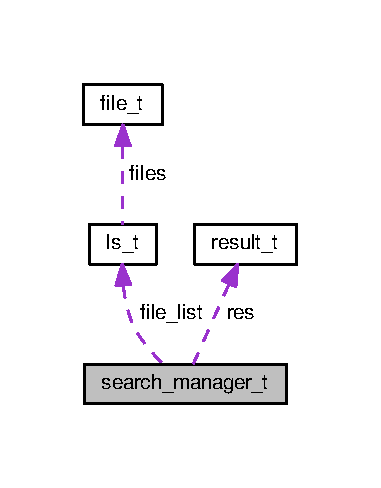
\includegraphics[width=183pt]{d6/d51/structsearch__manager__t__coll__graph}
\end{center}
\end{figure}
\subsection*{Attributi pubblici}
\begin{DoxyCompactItemize}
\item 
pthread\+\_\+t $\ast$ \hyperlink{structsearch__manager__t_abac9106caf0478276fc6cf288d30917c}{threads}
\item 
\hyperlink{structls__t}{ls\+\_\+t} $\ast$ \hyperlink{structsearch__manager__t_a7f1f64c246b3827f179dd96c678722cf}{file\+\_\+list}
\item 
\hyperlink{structresult__t}{result\+\_\+t} \hyperlink{structsearch__manager__t_ae71a7eb74a2af2e9f3ea2ab7de643139}{res}
\item 
char $\ast$ \hyperlink{structsearch__manager__t_ad36bf1b5a95e84275ae96e106fc88b6c}{email}
\end{DoxyCompactItemize}


\subsection{Descrizione dettagliata}
Struct che rappresenta il manager dei thread atti a ricercare le password all\textquotesingle{}interno degli archivi. 

~\newline
Campi\+:~\newline
1) t -\/ Array di thread searcher/worker;~\newline
2) file\+\_\+list -\/ Lista degli archivi in cui cercare;~\newline
3) res -\/ Password che corrispondo all\textquotesingle{}email dell\textquotesingle{}utente;~\newline
4) email -\/ Email inserita dall\textquotesingle{}utente. 

\subsection{Documentazione dei membri dato}
\mbox{\Hypertarget{structsearch__manager__t_ad36bf1b5a95e84275ae96e106fc88b6c}\label{structsearch__manager__t_ad36bf1b5a95e84275ae96e106fc88b6c}} 
\index{search\+\_\+manager\+\_\+t@{search\+\_\+manager\+\_\+t}!email@{email}}
\index{email@{email}!search\+\_\+manager\+\_\+t@{search\+\_\+manager\+\_\+t}}
\subsubsection{\texorpdfstring{email}{email}}
{\footnotesize\ttfamily char$\ast$ search\+\_\+manager\+\_\+t\+::email}

\mbox{\Hypertarget{structsearch__manager__t_a7f1f64c246b3827f179dd96c678722cf}\label{structsearch__manager__t_a7f1f64c246b3827f179dd96c678722cf}} 
\index{search\+\_\+manager\+\_\+t@{search\+\_\+manager\+\_\+t}!file\+\_\+list@{file\+\_\+list}}
\index{file\+\_\+list@{file\+\_\+list}!search\+\_\+manager\+\_\+t@{search\+\_\+manager\+\_\+t}}
\subsubsection{\texorpdfstring{file\+\_\+list}{file\_list}}
{\footnotesize\ttfamily \hyperlink{structls__t}{ls\+\_\+t}$\ast$ search\+\_\+manager\+\_\+t\+::file\+\_\+list}

\mbox{\Hypertarget{structsearch__manager__t_ae71a7eb74a2af2e9f3ea2ab7de643139}\label{structsearch__manager__t_ae71a7eb74a2af2e9f3ea2ab7de643139}} 
\index{search\+\_\+manager\+\_\+t@{search\+\_\+manager\+\_\+t}!res@{res}}
\index{res@{res}!search\+\_\+manager\+\_\+t@{search\+\_\+manager\+\_\+t}}
\subsubsection{\texorpdfstring{res}{res}}
{\footnotesize\ttfamily \hyperlink{structresult__t}{result\+\_\+t} search\+\_\+manager\+\_\+t\+::res}

\mbox{\Hypertarget{structsearch__manager__t_abac9106caf0478276fc6cf288d30917c}\label{structsearch__manager__t_abac9106caf0478276fc6cf288d30917c}} 
\index{search\+\_\+manager\+\_\+t@{search\+\_\+manager\+\_\+t}!threads@{threads}}
\index{threads@{threads}!search\+\_\+manager\+\_\+t@{search\+\_\+manager\+\_\+t}}
\subsubsection{\texorpdfstring{threads}{threads}}
{\footnotesize\ttfamily pthread\+\_\+t$\ast$ search\+\_\+manager\+\_\+t\+::threads}



La documentazione per questa struct è stata generata a partire dal seguente file\+:\begin{DoxyCompactItemize}
\item 
\hyperlink{data_8h}{data.\+h}\end{DoxyCompactItemize}

\hypertarget{structsettings__t}{}\section{Riferimenti per la struct settings\+\_\+t}
\label{structsettings__t}\index{settings\+\_\+t@{settings\+\_\+t}}


Struct contenente le impostazioni di gioco.  




{\ttfamily \#include $<$data.\+h$>$}

\subsection*{Attributi pubblici}
\begin{DoxyCompactItemize}
\item 
\hyperlink{data_8h_a56839c56ca6deb3cff5e21540ddb8218}{enable\+\_\+t} \hyperlink{structsettings__t_a2aa1ff1ddeee8e7ac3d1e544af1c2d67}{sound}
\item 
\hyperlink{data_8h_a56839c56ca6deb3cff5e21540ddb8218}{enable\+\_\+t} \hyperlink{structsettings__t_a4b0508385c16a4e5aeb4bf8b8f5cf6fe}{music}
\item 
bool \hyperlink{structsettings__t_a824c2f3df8afc1c1823769065bd6eeb3}{visible\+\_\+hints}
\end{DoxyCompactItemize}


\subsection{Descrizione dettagliata}
Struct contenente le impostazioni di gioco. 

~\newline
Campi\+: ~\newline
2) sound -\/ Impostazione relativa agli effetti sonori (\mbox{[}O\+FF,ON\mbox{]}); ~\newline
3) music -\/ Impostazione relativa alla musica (\mbox{[}O\+FF,ON\mbox{]}); ~\newline
4) visible\+\_\+hints -\/ Se \char`\"{}true\char`\"{}, i suggerimenti presenti sulla schermata di gioco risultano essere visibili. 

\subsection{Documentazione dei membri dato}
\mbox{\Hypertarget{structsettings__t_a4b0508385c16a4e5aeb4bf8b8f5cf6fe}\label{structsettings__t_a4b0508385c16a4e5aeb4bf8b8f5cf6fe}} 
\index{settings\+\_\+t@{settings\+\_\+t}!music@{music}}
\index{music@{music}!settings\+\_\+t@{settings\+\_\+t}}
\subsubsection{\texorpdfstring{music}{music}}
{\footnotesize\ttfamily \hyperlink{data_8h_a56839c56ca6deb3cff5e21540ddb8218}{enable\+\_\+t} settings\+\_\+t\+::music}

\mbox{\Hypertarget{structsettings__t_a2aa1ff1ddeee8e7ac3d1e544af1c2d67}\label{structsettings__t_a2aa1ff1ddeee8e7ac3d1e544af1c2d67}} 
\index{settings\+\_\+t@{settings\+\_\+t}!sound@{sound}}
\index{sound@{sound}!settings\+\_\+t@{settings\+\_\+t}}
\subsubsection{\texorpdfstring{sound}{sound}}
{\footnotesize\ttfamily \hyperlink{data_8h_a56839c56ca6deb3cff5e21540ddb8218}{enable\+\_\+t} settings\+\_\+t\+::sound}

\mbox{\Hypertarget{structsettings__t_a824c2f3df8afc1c1823769065bd6eeb3}\label{structsettings__t_a824c2f3df8afc1c1823769065bd6eeb3}} 
\index{settings\+\_\+t@{settings\+\_\+t}!visible\+\_\+hints@{visible\+\_\+hints}}
\index{visible\+\_\+hints@{visible\+\_\+hints}!settings\+\_\+t@{settings\+\_\+t}}
\subsubsection{\texorpdfstring{visible\+\_\+hints}{visible\_hints}}
{\footnotesize\ttfamily bool settings\+\_\+t\+::visible\+\_\+hints}



La documentazione per questa struct è stata generata a partire dal seguente file\+:\begin{DoxyCompactItemize}
\item 
\hyperlink{data_8h}{data.\+h}\end{DoxyCompactItemize}

\hypertarget{structshooter__t}{}\section{Riferimenti per la struct shooter\+\_\+t}
\label{structshooter__t}\index{shooter\+\_\+t@{shooter\+\_\+t}}


Struct contenente le informazioni relative al singolo proiettile.  




{\ttfamily \#include $<$data.\+h$>$}

\subsection*{Attributi pubblici}
\begin{DoxyCompactItemize}
\item 
float \hyperlink{structshooter__t_aede1685d00f485e9f0ed40279f3d147e}{x}
\item 
float \hyperlink{structshooter__t_adb6e42adc6b761f77c23208379a77711}{y}
\item 
float \hyperlink{structshooter__t_a958ea335a4ec8e592edb6ba8c927d511}{slope}
\item 
float \hyperlink{structshooter__t_a9e2043ccd69d180eca3f1b2b2b0fcaff}{radius}
\end{DoxyCompactItemize}


\subsection{Descrizione dettagliata}
Struct contenente le informazioni relative al singolo proiettile. 

~\newline
Campi\+: ~\newline
1) x -\/ Ascissa della navicella (centro del display); ~\newline
2) y -\/ Ordinata della navicella (centro del display); ~\newline
3) slope -\/ Angolo di rotazione della \char`\"{}testa\char`\"{} della navicella; ~\newline
4) radius -\/ Raggio della navicella. 

\subsection{Documentazione dei membri dato}
\mbox{\Hypertarget{structshooter__t_a9e2043ccd69d180eca3f1b2b2b0fcaff}\label{structshooter__t_a9e2043ccd69d180eca3f1b2b2b0fcaff}} 
\index{shooter\+\_\+t@{shooter\+\_\+t}!radius@{radius}}
\index{radius@{radius}!shooter\+\_\+t@{shooter\+\_\+t}}
\subsubsection{\texorpdfstring{radius}{radius}}
{\footnotesize\ttfamily float shooter\+\_\+t\+::radius}

\mbox{\Hypertarget{structshooter__t_a958ea335a4ec8e592edb6ba8c927d511}\label{structshooter__t_a958ea335a4ec8e592edb6ba8c927d511}} 
\index{shooter\+\_\+t@{shooter\+\_\+t}!slope@{slope}}
\index{slope@{slope}!shooter\+\_\+t@{shooter\+\_\+t}}
\subsubsection{\texorpdfstring{slope}{slope}}
{\footnotesize\ttfamily float shooter\+\_\+t\+::slope}

\mbox{\Hypertarget{structshooter__t_aede1685d00f485e9f0ed40279f3d147e}\label{structshooter__t_aede1685d00f485e9f0ed40279f3d147e}} 
\index{shooter\+\_\+t@{shooter\+\_\+t}!x@{x}}
\index{x@{x}!shooter\+\_\+t@{shooter\+\_\+t}}
\subsubsection{\texorpdfstring{x}{x}}
{\footnotesize\ttfamily float shooter\+\_\+t\+::x}

\mbox{\Hypertarget{structshooter__t_adb6e42adc6b761f77c23208379a77711}\label{structshooter__t_adb6e42adc6b761f77c23208379a77711}} 
\index{shooter\+\_\+t@{shooter\+\_\+t}!y@{y}}
\index{y@{y}!shooter\+\_\+t@{shooter\+\_\+t}}
\subsubsection{\texorpdfstring{y}{y}}
{\footnotesize\ttfamily float shooter\+\_\+t\+::y}



La documentazione per questa struct è stata generata a partire dal seguente file\+:\begin{DoxyCompactItemize}
\item 
\hyperlink{data_8h}{data.\+h}\end{DoxyCompactItemize}

\hypertarget{structthread__manager__t}{}\section{Riferimenti per la struct thread\+\_\+manager\+\_\+t}
\label{structthread__manager__t}\index{thread\+\_\+manager\+\_\+t@{thread\+\_\+manager\+\_\+t}}


Struct che contiene le variabili di sincronizzazione del gioco.  




{\ttfamily \#include $<$data.\+h$>$}



Diagramma di collaborazione per thread\+\_\+manager\+\_\+t\+:\nopagebreak
\begin{figure}[H]
\begin{center}
\leavevmode
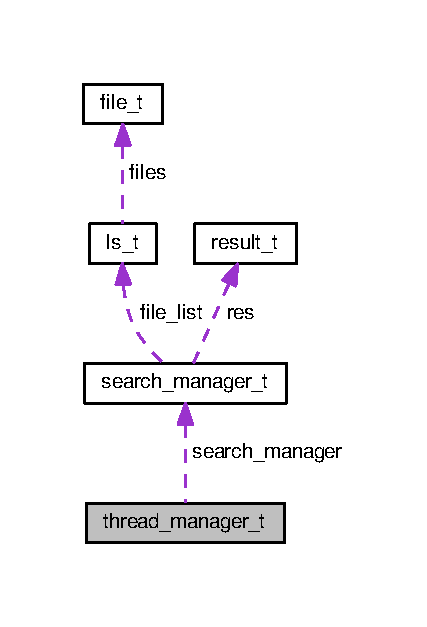
\includegraphics[width=205pt]{d8/df3/structthread__manager__t__coll__graph}
\end{center}
\end{figure}
\subsection*{Attributi pubblici}
\begin{DoxyCompactItemize}
\item 
\hyperlink{structsearch__manager__t}{search\+\_\+manager\+\_\+t} \hyperlink{structthread__manager__t_a1020a46c9471ad522d62cd82f212967d}{search\+\_\+manager}
\item 
pthread\+\_\+t \hyperlink{structthread__manager__t_a0d5c8b3e690252132fcf05abf7b03bca}{searcher\+\_\+thread}
\item 
pthread\+\_\+t \hyperlink{structthread__manager__t_afe6523e46806390d78b6e33c8298b50c}{spawner\+\_\+thread}
\item 
sem\+\_\+t \hyperlink{structthread__manager__t_ae21d407363c3091b08d020ee91d2fb19}{searcher\+\_\+sem}
\item 
sem\+\_\+t \hyperlink{structthread__manager__t_add09eb9696fcde21f6ea575747dd9bc6}{consumer\+\_\+sem}
\item 
pthread\+\_\+cond\+\_\+t \hyperlink{structthread__manager__t_a3d2875e19825c1177a202dbee945dda7}{spawn\+\_\+cond}
\item 
pthread\+\_\+mutex\+\_\+t \hyperlink{structthread__manager__t_a0c6481fe0c14e7061e39e7c71a080a72}{spawn\+\_\+mutex}
\item 
pthread\+\_\+mutex\+\_\+t \hyperlink{structthread__manager__t_acbf655b8885eb6344c889df3bdc04914}{words\+\_\+buffer\+\_\+mutex}
\item 
pthread\+\_\+cond\+\_\+t \hyperlink{structthread__manager__t_adc9c0bc7d1a31425ee832c85e2568a4c}{gameover\+\_\+cond}
\item 
pthread\+\_\+mutex\+\_\+t \hyperlink{structthread__manager__t_af7c55eacef734d190ef5c8ca4bd0a047}{gameover\+\_\+mutex}
\item 
pthread\+\_\+mutex\+\_\+t \hyperlink{structthread__manager__t_ab2460282f6fd131b9d3f0aacb9ddbf72}{search\+\_\+result\+\_\+mutex}
\end{DoxyCompactItemize}


\subsection{Descrizione dettagliata}
Struct che contiene le variabili di sincronizzazione del gioco. 

~\newline
Campi\+: 1) search\+\_\+manager -\/ struct che contiene le informazioni per la ricerca dentro gli archivi; 2) searcher\+\_\+thread -\/ thread che si occupa della ricerca delle informazioni (producer); 3) spawner\+\_\+thread -\/ thread che si occupa di fornire le parole al gioco (consumer); 4) searcher\+\_\+sem -\/ semaforo privato per i producer; 5) consumer\+\_\+sem -\/ semaforo privato per i consumer; 6) spawn\+\_\+cond -\/ condition per la sincronizzazione dello spawner thread; 7) spawn\+\_\+mutex -\/ mutex per la sincronizzazione dello spawner thread; 8) words\+\_\+buffer\+\_\+mutex -\/ mutex per gestire il buffer condiviso; 9) gameover\+\_\+cond -\/ condition per la sincronizzazione dei threads con il gioco principale; 10) gameover\+\_\+mutex -\/ mutex per la sincronizzazione dei threads con il gioco principale; 11) search\+\_\+result\+\_\+mutex -\/ mutex per gestire la mutua esclusione sui risultati della ricerca; 

\subsection{Documentazione dei membri dato}
\mbox{\Hypertarget{structthread__manager__t_add09eb9696fcde21f6ea575747dd9bc6}\label{structthread__manager__t_add09eb9696fcde21f6ea575747dd9bc6}} 
\index{thread\+\_\+manager\+\_\+t@{thread\+\_\+manager\+\_\+t}!consumer\+\_\+sem@{consumer\+\_\+sem}}
\index{consumer\+\_\+sem@{consumer\+\_\+sem}!thread\+\_\+manager\+\_\+t@{thread\+\_\+manager\+\_\+t}}
\subsubsection{\texorpdfstring{consumer\+\_\+sem}{consumer\_sem}}
{\footnotesize\ttfamily sem\+\_\+t thread\+\_\+manager\+\_\+t\+::consumer\+\_\+sem}

\mbox{\Hypertarget{structthread__manager__t_adc9c0bc7d1a31425ee832c85e2568a4c}\label{structthread__manager__t_adc9c0bc7d1a31425ee832c85e2568a4c}} 
\index{thread\+\_\+manager\+\_\+t@{thread\+\_\+manager\+\_\+t}!gameover\+\_\+cond@{gameover\+\_\+cond}}
\index{gameover\+\_\+cond@{gameover\+\_\+cond}!thread\+\_\+manager\+\_\+t@{thread\+\_\+manager\+\_\+t}}
\subsubsection{\texorpdfstring{gameover\+\_\+cond}{gameover\_cond}}
{\footnotesize\ttfamily pthread\+\_\+cond\+\_\+t thread\+\_\+manager\+\_\+t\+::gameover\+\_\+cond}

\mbox{\Hypertarget{structthread__manager__t_af7c55eacef734d190ef5c8ca4bd0a047}\label{structthread__manager__t_af7c55eacef734d190ef5c8ca4bd0a047}} 
\index{thread\+\_\+manager\+\_\+t@{thread\+\_\+manager\+\_\+t}!gameover\+\_\+mutex@{gameover\+\_\+mutex}}
\index{gameover\+\_\+mutex@{gameover\+\_\+mutex}!thread\+\_\+manager\+\_\+t@{thread\+\_\+manager\+\_\+t}}
\subsubsection{\texorpdfstring{gameover\+\_\+mutex}{gameover\_mutex}}
{\footnotesize\ttfamily pthread\+\_\+mutex\+\_\+t thread\+\_\+manager\+\_\+t\+::gameover\+\_\+mutex}

\mbox{\Hypertarget{structthread__manager__t_a1020a46c9471ad522d62cd82f212967d}\label{structthread__manager__t_a1020a46c9471ad522d62cd82f212967d}} 
\index{thread\+\_\+manager\+\_\+t@{thread\+\_\+manager\+\_\+t}!search\+\_\+manager@{search\+\_\+manager}}
\index{search\+\_\+manager@{search\+\_\+manager}!thread\+\_\+manager\+\_\+t@{thread\+\_\+manager\+\_\+t}}
\subsubsection{\texorpdfstring{search\+\_\+manager}{search\_manager}}
{\footnotesize\ttfamily \hyperlink{structsearch__manager__t}{search\+\_\+manager\+\_\+t} thread\+\_\+manager\+\_\+t\+::search\+\_\+manager}

\mbox{\Hypertarget{structthread__manager__t_ab2460282f6fd131b9d3f0aacb9ddbf72}\label{structthread__manager__t_ab2460282f6fd131b9d3f0aacb9ddbf72}} 
\index{thread\+\_\+manager\+\_\+t@{thread\+\_\+manager\+\_\+t}!search\+\_\+result\+\_\+mutex@{search\+\_\+result\+\_\+mutex}}
\index{search\+\_\+result\+\_\+mutex@{search\+\_\+result\+\_\+mutex}!thread\+\_\+manager\+\_\+t@{thread\+\_\+manager\+\_\+t}}
\subsubsection{\texorpdfstring{search\+\_\+result\+\_\+mutex}{search\_result\_mutex}}
{\footnotesize\ttfamily pthread\+\_\+mutex\+\_\+t thread\+\_\+manager\+\_\+t\+::search\+\_\+result\+\_\+mutex}

\mbox{\Hypertarget{structthread__manager__t_ae21d407363c3091b08d020ee91d2fb19}\label{structthread__manager__t_ae21d407363c3091b08d020ee91d2fb19}} 
\index{thread\+\_\+manager\+\_\+t@{thread\+\_\+manager\+\_\+t}!searcher\+\_\+sem@{searcher\+\_\+sem}}
\index{searcher\+\_\+sem@{searcher\+\_\+sem}!thread\+\_\+manager\+\_\+t@{thread\+\_\+manager\+\_\+t}}
\subsubsection{\texorpdfstring{searcher\+\_\+sem}{searcher\_sem}}
{\footnotesize\ttfamily sem\+\_\+t thread\+\_\+manager\+\_\+t\+::searcher\+\_\+sem}

\mbox{\Hypertarget{structthread__manager__t_a0d5c8b3e690252132fcf05abf7b03bca}\label{structthread__manager__t_a0d5c8b3e690252132fcf05abf7b03bca}} 
\index{thread\+\_\+manager\+\_\+t@{thread\+\_\+manager\+\_\+t}!searcher\+\_\+thread@{searcher\+\_\+thread}}
\index{searcher\+\_\+thread@{searcher\+\_\+thread}!thread\+\_\+manager\+\_\+t@{thread\+\_\+manager\+\_\+t}}
\subsubsection{\texorpdfstring{searcher\+\_\+thread}{searcher\_thread}}
{\footnotesize\ttfamily pthread\+\_\+t thread\+\_\+manager\+\_\+t\+::searcher\+\_\+thread}

\mbox{\Hypertarget{structthread__manager__t_a3d2875e19825c1177a202dbee945dda7}\label{structthread__manager__t_a3d2875e19825c1177a202dbee945dda7}} 
\index{thread\+\_\+manager\+\_\+t@{thread\+\_\+manager\+\_\+t}!spawn\+\_\+cond@{spawn\+\_\+cond}}
\index{spawn\+\_\+cond@{spawn\+\_\+cond}!thread\+\_\+manager\+\_\+t@{thread\+\_\+manager\+\_\+t}}
\subsubsection{\texorpdfstring{spawn\+\_\+cond}{spawn\_cond}}
{\footnotesize\ttfamily pthread\+\_\+cond\+\_\+t thread\+\_\+manager\+\_\+t\+::spawn\+\_\+cond}

\mbox{\Hypertarget{structthread__manager__t_a0c6481fe0c14e7061e39e7c71a080a72}\label{structthread__manager__t_a0c6481fe0c14e7061e39e7c71a080a72}} 
\index{thread\+\_\+manager\+\_\+t@{thread\+\_\+manager\+\_\+t}!spawn\+\_\+mutex@{spawn\+\_\+mutex}}
\index{spawn\+\_\+mutex@{spawn\+\_\+mutex}!thread\+\_\+manager\+\_\+t@{thread\+\_\+manager\+\_\+t}}
\subsubsection{\texorpdfstring{spawn\+\_\+mutex}{spawn\_mutex}}
{\footnotesize\ttfamily pthread\+\_\+mutex\+\_\+t thread\+\_\+manager\+\_\+t\+::spawn\+\_\+mutex}

\mbox{\Hypertarget{structthread__manager__t_afe6523e46806390d78b6e33c8298b50c}\label{structthread__manager__t_afe6523e46806390d78b6e33c8298b50c}} 
\index{thread\+\_\+manager\+\_\+t@{thread\+\_\+manager\+\_\+t}!spawner\+\_\+thread@{spawner\+\_\+thread}}
\index{spawner\+\_\+thread@{spawner\+\_\+thread}!thread\+\_\+manager\+\_\+t@{thread\+\_\+manager\+\_\+t}}
\subsubsection{\texorpdfstring{spawner\+\_\+thread}{spawner\_thread}}
{\footnotesize\ttfamily pthread\+\_\+t thread\+\_\+manager\+\_\+t\+::spawner\+\_\+thread}

\mbox{\Hypertarget{structthread__manager__t_acbf655b8885eb6344c889df3bdc04914}\label{structthread__manager__t_acbf655b8885eb6344c889df3bdc04914}} 
\index{thread\+\_\+manager\+\_\+t@{thread\+\_\+manager\+\_\+t}!words\+\_\+buffer\+\_\+mutex@{words\+\_\+buffer\+\_\+mutex}}
\index{words\+\_\+buffer\+\_\+mutex@{words\+\_\+buffer\+\_\+mutex}!thread\+\_\+manager\+\_\+t@{thread\+\_\+manager\+\_\+t}}
\subsubsection{\texorpdfstring{words\+\_\+buffer\+\_\+mutex}{words\_buffer\_mutex}}
{\footnotesize\ttfamily pthread\+\_\+mutex\+\_\+t thread\+\_\+manager\+\_\+t\+::words\+\_\+buffer\+\_\+mutex}



La documentazione per questa struct è stata generata a partire dal seguente file\+:\begin{DoxyCompactItemize}
\item 
\hyperlink{data_8h}{data.\+h}\end{DoxyCompactItemize}

\hypertarget{structusr__gv__t}{}\section{Riferimenti per la struct usr\+\_\+gv\+\_\+t}
\label{structusr__gv__t}\index{usr\+\_\+gv\+\_\+t@{usr\+\_\+gv\+\_\+t}}


Struct relativo alle proporzioni grafiche della schermata di fine partita.  




{\ttfamily \#include $<$data.\+h$>$}

\subsection*{Attributi pubblici}
\begin{DoxyCompactItemize}
\item 
float \hyperlink{structusr__gv__t_a6771f8678ff677e94db59138b3cb322d}{U\+S\+E\+R\+N\+A\+M\+E\+\_\+\+B\+L\+O\+C\+K\+\_\+\+T\+O\+P\+\_\+\+O\+F\+F\+S\+ET}
\item 
float \hyperlink{structusr__gv__t_ad9f2d3a263b00fe3318e7d6e58937c6f}{E\+N\+T\+E\+R\+\_\+\+L\+E\+F\+T\+\_\+\+O\+F\+F\+S\+ET}
\item 
float \hyperlink{structusr__gv__t_afba7f0e6539eb98ac504e466d8ae7497}{E\+N\+T\+E\+R\+\_\+\+T\+O\+P\+\_\+\+O\+F\+F\+S\+ET}
\item 
float \hyperlink{structusr__gv__t_a4f72cddaa03f366b05af169b6cc6e57f}{E\+N\+T\+E\+R\+\_\+\+W\+I\+D\+TH}
\item 
float \hyperlink{structusr__gv__t_a5630e2937541909c51c67e17a9006fe0}{E\+N\+T\+E\+R\+\_\+\+H\+E\+I\+G\+HT}
\item 
int \hyperlink{structusr__gv__t_a9f98fe0caf526ac025f34b2767f763d7}{U\+S\+E\+R\+N\+A\+M\+E\+\_\+\+F\+O\+N\+T\+S\+I\+ZE}
\item 
int \hyperlink{structusr__gv__t_a56f1871d5de77a092900916d70d62d28}{S\+T\+A\+T\+S\+\_\+\+F\+O\+N\+T\+S\+I\+ZE}
\item 
int \hyperlink{structusr__gv__t_a5f34421e0029b76550de152894ebf2ef}{E\+N\+T\+E\+R\+\_\+\+F\+O\+N\+T\+S\+I\+ZE}
\end{DoxyCompactItemize}


\subsection{Descrizione dettagliata}
Struct relativo alle proporzioni grafiche della schermata di fine partita. 

\subsection{Documentazione dei membri dato}
\mbox{\Hypertarget{structusr__gv__t_a5f34421e0029b76550de152894ebf2ef}\label{structusr__gv__t_a5f34421e0029b76550de152894ebf2ef}} 
\index{usr\+\_\+gv\+\_\+t@{usr\+\_\+gv\+\_\+t}!E\+N\+T\+E\+R\+\_\+\+F\+O\+N\+T\+S\+I\+ZE@{E\+N\+T\+E\+R\+\_\+\+F\+O\+N\+T\+S\+I\+ZE}}
\index{E\+N\+T\+E\+R\+\_\+\+F\+O\+N\+T\+S\+I\+ZE@{E\+N\+T\+E\+R\+\_\+\+F\+O\+N\+T\+S\+I\+ZE}!usr\+\_\+gv\+\_\+t@{usr\+\_\+gv\+\_\+t}}
\subsubsection{\texorpdfstring{E\+N\+T\+E\+R\+\_\+\+F\+O\+N\+T\+S\+I\+ZE}{ENTER\_FONTSIZE}}
{\footnotesize\ttfamily int usr\+\_\+gv\+\_\+t\+::\+E\+N\+T\+E\+R\+\_\+\+F\+O\+N\+T\+S\+I\+ZE}

\mbox{\Hypertarget{structusr__gv__t_a5630e2937541909c51c67e17a9006fe0}\label{structusr__gv__t_a5630e2937541909c51c67e17a9006fe0}} 
\index{usr\+\_\+gv\+\_\+t@{usr\+\_\+gv\+\_\+t}!E\+N\+T\+E\+R\+\_\+\+H\+E\+I\+G\+HT@{E\+N\+T\+E\+R\+\_\+\+H\+E\+I\+G\+HT}}
\index{E\+N\+T\+E\+R\+\_\+\+H\+E\+I\+G\+HT@{E\+N\+T\+E\+R\+\_\+\+H\+E\+I\+G\+HT}!usr\+\_\+gv\+\_\+t@{usr\+\_\+gv\+\_\+t}}
\subsubsection{\texorpdfstring{E\+N\+T\+E\+R\+\_\+\+H\+E\+I\+G\+HT}{ENTER\_HEIGHT}}
{\footnotesize\ttfamily float usr\+\_\+gv\+\_\+t\+::\+E\+N\+T\+E\+R\+\_\+\+H\+E\+I\+G\+HT}

\mbox{\Hypertarget{structusr__gv__t_ad9f2d3a263b00fe3318e7d6e58937c6f}\label{structusr__gv__t_ad9f2d3a263b00fe3318e7d6e58937c6f}} 
\index{usr\+\_\+gv\+\_\+t@{usr\+\_\+gv\+\_\+t}!E\+N\+T\+E\+R\+\_\+\+L\+E\+F\+T\+\_\+\+O\+F\+F\+S\+ET@{E\+N\+T\+E\+R\+\_\+\+L\+E\+F\+T\+\_\+\+O\+F\+F\+S\+ET}}
\index{E\+N\+T\+E\+R\+\_\+\+L\+E\+F\+T\+\_\+\+O\+F\+F\+S\+ET@{E\+N\+T\+E\+R\+\_\+\+L\+E\+F\+T\+\_\+\+O\+F\+F\+S\+ET}!usr\+\_\+gv\+\_\+t@{usr\+\_\+gv\+\_\+t}}
\subsubsection{\texorpdfstring{E\+N\+T\+E\+R\+\_\+\+L\+E\+F\+T\+\_\+\+O\+F\+F\+S\+ET}{ENTER\_LEFT\_OFFSET}}
{\footnotesize\ttfamily float usr\+\_\+gv\+\_\+t\+::\+E\+N\+T\+E\+R\+\_\+\+L\+E\+F\+T\+\_\+\+O\+F\+F\+S\+ET}

\mbox{\Hypertarget{structusr__gv__t_afba7f0e6539eb98ac504e466d8ae7497}\label{structusr__gv__t_afba7f0e6539eb98ac504e466d8ae7497}} 
\index{usr\+\_\+gv\+\_\+t@{usr\+\_\+gv\+\_\+t}!E\+N\+T\+E\+R\+\_\+\+T\+O\+P\+\_\+\+O\+F\+F\+S\+ET@{E\+N\+T\+E\+R\+\_\+\+T\+O\+P\+\_\+\+O\+F\+F\+S\+ET}}
\index{E\+N\+T\+E\+R\+\_\+\+T\+O\+P\+\_\+\+O\+F\+F\+S\+ET@{E\+N\+T\+E\+R\+\_\+\+T\+O\+P\+\_\+\+O\+F\+F\+S\+ET}!usr\+\_\+gv\+\_\+t@{usr\+\_\+gv\+\_\+t}}
\subsubsection{\texorpdfstring{E\+N\+T\+E\+R\+\_\+\+T\+O\+P\+\_\+\+O\+F\+F\+S\+ET}{ENTER\_TOP\_OFFSET}}
{\footnotesize\ttfamily float usr\+\_\+gv\+\_\+t\+::\+E\+N\+T\+E\+R\+\_\+\+T\+O\+P\+\_\+\+O\+F\+F\+S\+ET}

\mbox{\Hypertarget{structusr__gv__t_a4f72cddaa03f366b05af169b6cc6e57f}\label{structusr__gv__t_a4f72cddaa03f366b05af169b6cc6e57f}} 
\index{usr\+\_\+gv\+\_\+t@{usr\+\_\+gv\+\_\+t}!E\+N\+T\+E\+R\+\_\+\+W\+I\+D\+TH@{E\+N\+T\+E\+R\+\_\+\+W\+I\+D\+TH}}
\index{E\+N\+T\+E\+R\+\_\+\+W\+I\+D\+TH@{E\+N\+T\+E\+R\+\_\+\+W\+I\+D\+TH}!usr\+\_\+gv\+\_\+t@{usr\+\_\+gv\+\_\+t}}
\subsubsection{\texorpdfstring{E\+N\+T\+E\+R\+\_\+\+W\+I\+D\+TH}{ENTER\_WIDTH}}
{\footnotesize\ttfamily float usr\+\_\+gv\+\_\+t\+::\+E\+N\+T\+E\+R\+\_\+\+W\+I\+D\+TH}

\mbox{\Hypertarget{structusr__gv__t_a56f1871d5de77a092900916d70d62d28}\label{structusr__gv__t_a56f1871d5de77a092900916d70d62d28}} 
\index{usr\+\_\+gv\+\_\+t@{usr\+\_\+gv\+\_\+t}!S\+T\+A\+T\+S\+\_\+\+F\+O\+N\+T\+S\+I\+ZE@{S\+T\+A\+T\+S\+\_\+\+F\+O\+N\+T\+S\+I\+ZE}}
\index{S\+T\+A\+T\+S\+\_\+\+F\+O\+N\+T\+S\+I\+ZE@{S\+T\+A\+T\+S\+\_\+\+F\+O\+N\+T\+S\+I\+ZE}!usr\+\_\+gv\+\_\+t@{usr\+\_\+gv\+\_\+t}}
\subsubsection{\texorpdfstring{S\+T\+A\+T\+S\+\_\+\+F\+O\+N\+T\+S\+I\+ZE}{STATS\_FONTSIZE}}
{\footnotesize\ttfamily int usr\+\_\+gv\+\_\+t\+::\+S\+T\+A\+T\+S\+\_\+\+F\+O\+N\+T\+S\+I\+ZE}

\mbox{\Hypertarget{structusr__gv__t_a6771f8678ff677e94db59138b3cb322d}\label{structusr__gv__t_a6771f8678ff677e94db59138b3cb322d}} 
\index{usr\+\_\+gv\+\_\+t@{usr\+\_\+gv\+\_\+t}!U\+S\+E\+R\+N\+A\+M\+E\+\_\+\+B\+L\+O\+C\+K\+\_\+\+T\+O\+P\+\_\+\+O\+F\+F\+S\+ET@{U\+S\+E\+R\+N\+A\+M\+E\+\_\+\+B\+L\+O\+C\+K\+\_\+\+T\+O\+P\+\_\+\+O\+F\+F\+S\+ET}}
\index{U\+S\+E\+R\+N\+A\+M\+E\+\_\+\+B\+L\+O\+C\+K\+\_\+\+T\+O\+P\+\_\+\+O\+F\+F\+S\+ET@{U\+S\+E\+R\+N\+A\+M\+E\+\_\+\+B\+L\+O\+C\+K\+\_\+\+T\+O\+P\+\_\+\+O\+F\+F\+S\+ET}!usr\+\_\+gv\+\_\+t@{usr\+\_\+gv\+\_\+t}}
\subsubsection{\texorpdfstring{U\+S\+E\+R\+N\+A\+M\+E\+\_\+\+B\+L\+O\+C\+K\+\_\+\+T\+O\+P\+\_\+\+O\+F\+F\+S\+ET}{USERNAME\_BLOCK\_TOP\_OFFSET}}
{\footnotesize\ttfamily float usr\+\_\+gv\+\_\+t\+::\+U\+S\+E\+R\+N\+A\+M\+E\+\_\+\+B\+L\+O\+C\+K\+\_\+\+T\+O\+P\+\_\+\+O\+F\+F\+S\+ET}

\mbox{\Hypertarget{structusr__gv__t_a9f98fe0caf526ac025f34b2767f763d7}\label{structusr__gv__t_a9f98fe0caf526ac025f34b2767f763d7}} 
\index{usr\+\_\+gv\+\_\+t@{usr\+\_\+gv\+\_\+t}!U\+S\+E\+R\+N\+A\+M\+E\+\_\+\+F\+O\+N\+T\+S\+I\+ZE@{U\+S\+E\+R\+N\+A\+M\+E\+\_\+\+F\+O\+N\+T\+S\+I\+ZE}}
\index{U\+S\+E\+R\+N\+A\+M\+E\+\_\+\+F\+O\+N\+T\+S\+I\+ZE@{U\+S\+E\+R\+N\+A\+M\+E\+\_\+\+F\+O\+N\+T\+S\+I\+ZE}!usr\+\_\+gv\+\_\+t@{usr\+\_\+gv\+\_\+t}}
\subsubsection{\texorpdfstring{U\+S\+E\+R\+N\+A\+M\+E\+\_\+\+F\+O\+N\+T\+S\+I\+ZE}{USERNAME\_FONTSIZE}}
{\footnotesize\ttfamily int usr\+\_\+gv\+\_\+t\+::\+U\+S\+E\+R\+N\+A\+M\+E\+\_\+\+F\+O\+N\+T\+S\+I\+ZE}



La documentazione per questa struct è stata generata a partire dal seguente file\+:\begin{DoxyCompactItemize}
\item 
\hyperlink{data_8h}{data.\+h}\end{DoxyCompactItemize}

\hypertarget{structwords__buffer__t}{}\section{Riferimenti per la struct words\+\_\+buffer\+\_\+t}
\label{structwords__buffer__t}\index{words\+\_\+buffer\+\_\+t@{words\+\_\+buffer\+\_\+t}}


Struct buffer che implementa l\textquotesingle{}architettura producer/consumer.  




{\ttfamily \#include $<$data.\+h$>$}

\subsection*{Attributi pubblici}
\begin{DoxyCompactItemize}
\item 
char $\ast$ \hyperlink{structwords__buffer__t_adf3a889cf3336fbf3bae9104f65e2969}{words} \mbox{[}\hyperlink{data_8h_abbb1a97343fdbf54e75f14fb83cb0a92}{N\+\_\+\+Q\+U\+E\+U\+ES}\mbox{]}
\item 
int \hyperlink{structwords__buffer__t_a86636af515bf8ca7b564e2c46ff24e28}{load}
\end{DoxyCompactItemize}


\subsection{Descrizione dettagliata}
Struct buffer che implementa l\textquotesingle{}architettura producer/consumer. 

\subsection{Documentazione dei membri dato}
\mbox{\Hypertarget{structwords__buffer__t_a86636af515bf8ca7b564e2c46ff24e28}\label{structwords__buffer__t_a86636af515bf8ca7b564e2c46ff24e28}} 
\index{words\+\_\+buffer\+\_\+t@{words\+\_\+buffer\+\_\+t}!load@{load}}
\index{load@{load}!words\+\_\+buffer\+\_\+t@{words\+\_\+buffer\+\_\+t}}
\subsubsection{\texorpdfstring{load}{load}}
{\footnotesize\ttfamily int words\+\_\+buffer\+\_\+t\+::load}

\mbox{\Hypertarget{structwords__buffer__t_adf3a889cf3336fbf3bae9104f65e2969}\label{structwords__buffer__t_adf3a889cf3336fbf3bae9104f65e2969}} 
\index{words\+\_\+buffer\+\_\+t@{words\+\_\+buffer\+\_\+t}!words@{words}}
\index{words@{words}!words\+\_\+buffer\+\_\+t@{words\+\_\+buffer\+\_\+t}}
\subsubsection{\texorpdfstring{words}{words}}
{\footnotesize\ttfamily char$\ast$ words\+\_\+buffer\+\_\+t\+::words\mbox{[}\hyperlink{data_8h_abbb1a97343fdbf54e75f14fb83cb0a92}{N\+\_\+\+Q\+U\+E\+U\+ES}\mbox{]}}



La documentazione per questa struct è stata generata a partire dal seguente file\+:\begin{DoxyCompactItemize}
\item 
\hyperlink{data_8h}{data.\+h}\end{DoxyCompactItemize}

\chapter{Documentazione dei file}
\hypertarget{archive__functions_8cpp}{}\section{Riferimenti per il file archive\+\_\+functions.\+cpp}
\label{archive__functions_8cpp}\index{archive\+\_\+functions.\+cpp@{archive\+\_\+functions.\+cpp}}
{\ttfamily \#include $<$stdio.\+h$>$}\newline
{\ttfamily \#include $<$string.\+h$>$}\newline
{\ttfamily \#include $<$dirent.\+h$>$}\newline
{\ttfamily \#include $<$malloc.\+h$>$}\newline
{\ttfamily \#include $<$archive.\+h$>$}\newline
{\ttfamily \#include $<$archive\+\_\+entry.\+h$>$}\newline
{\ttfamily \#include $<$stdlib.\+h$>$}\newline
{\ttfamily \#include $<$pthread.\+h$>$}\newline
{\ttfamily \#include $<$semaphore.\+h$>$}\newline
{\ttfamily \#include $<$cctype$>$}\newline
{\ttfamily \#include \char`\"{}archive\+\_\+functions.\+h\char`\"{}}\newline
Grafo delle dipendenze di inclusione per archive\+\_\+functions.\+cpp\+:\nopagebreak
\begin{figure}[H]
\begin{center}
\leavevmode
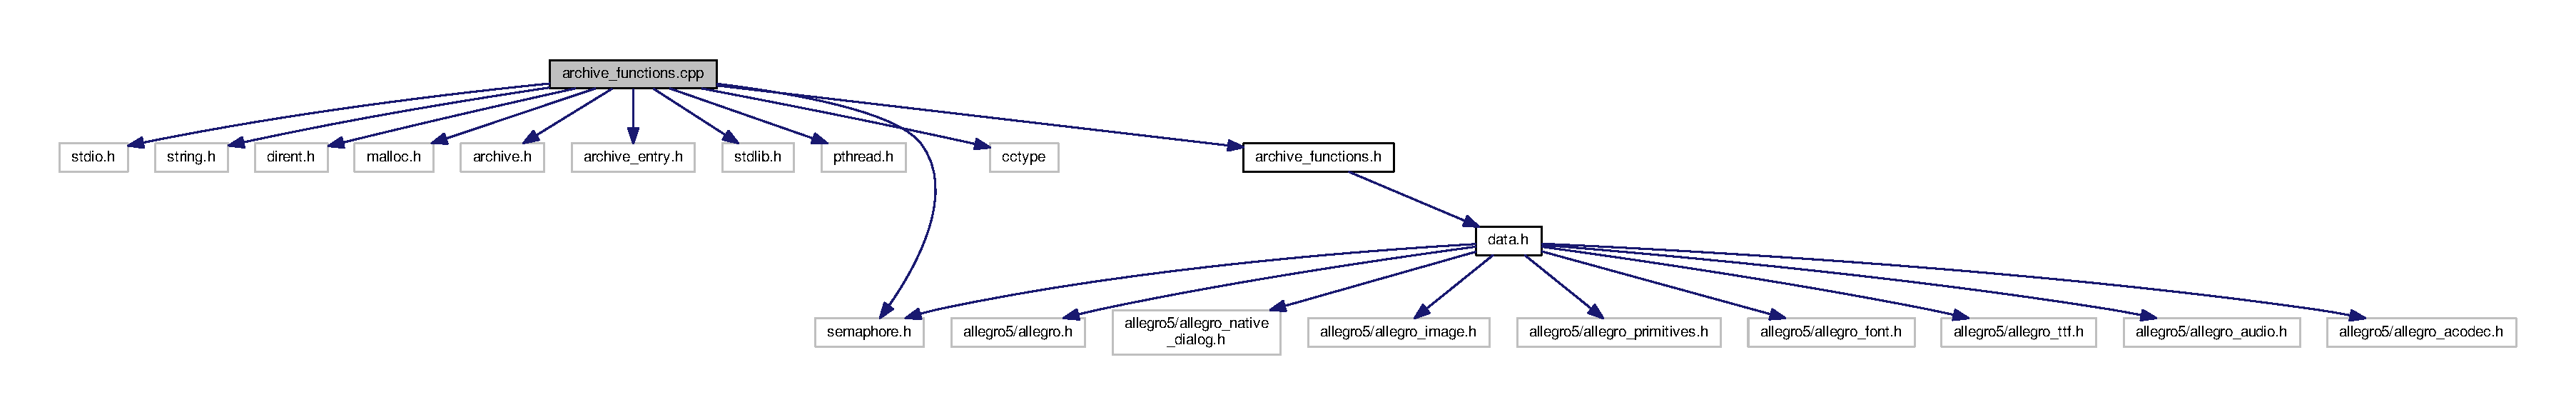
\includegraphics[width=350pt]{de/da7/archive__functions_8cpp__incl}
\end{center}
\end{figure}
\subsection*{Funzioni}
\begin{DoxyCompactItemize}
\item 
void $\ast$ \hyperlink{archive__functions_8cpp_a9f84e719a4e4079c5aad042930458381}{start\+\_\+searching} (void $\ast$search\+\_\+manager)
\begin{DoxyCompactList}\small\item\em Funzione che gestire i thread searcher e worker. \end{DoxyCompactList}\end{DoxyCompactItemize}


\subsection{Documentazione delle funzioni}
\mbox{\Hypertarget{archive__functions_8cpp_a9f84e719a4e4079c5aad042930458381}\label{archive__functions_8cpp_a9f84e719a4e4079c5aad042930458381}} 
\index{archive\+\_\+functions.\+cpp@{archive\+\_\+functions.\+cpp}!start\+\_\+searching@{start\+\_\+searching}}
\index{start\+\_\+searching@{start\+\_\+searching}!archive\+\_\+functions.\+cpp@{archive\+\_\+functions.\+cpp}}
\subsubsection{\texorpdfstring{start\+\_\+searching()}{start\_searching()}}
{\footnotesize\ttfamily void$\ast$ start\+\_\+searching (\begin{DoxyParamCaption}\item[{void $\ast$}]{search\+\_\+manager }\end{DoxyParamCaption})}



Funzione che gestire i thread searcher e worker. 

~\newline
Questi thread gestiscono la ricerca dell\textquotesingle{}email dello username all\textquotesingle{}interno delle collection. ~\newline
Parametri\+: ~\newline
1) search\+\_\+manager -\/ Variabile contenente le strutture per la sincronizzazione la ricerca. 
\hypertarget{archive__functions_8h}{}\section{Riferimenti per il file archive\+\_\+functions.\+h}
\label{archive__functions_8h}\index{archive\+\_\+functions.\+h@{archive\+\_\+functions.\+h}}
{\ttfamily \#include \char`\"{}data.\+h\char`\"{}}\newline
Grafo delle dipendenze di inclusione per archive\+\_\+functions.\+h\+:\nopagebreak
\begin{figure}[H]
\begin{center}
\leavevmode
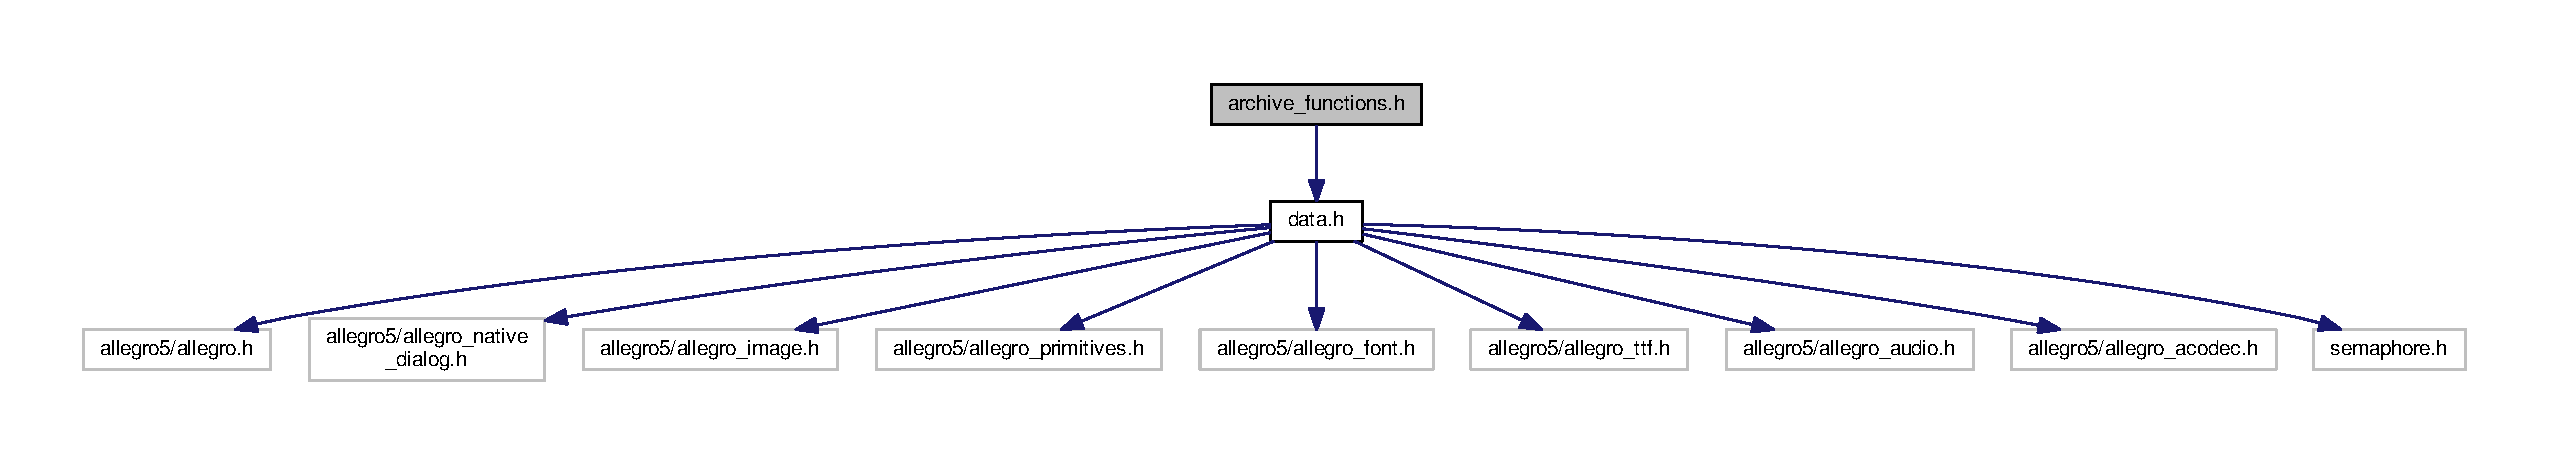
\includegraphics[width=350pt]{d8/db7/archive__functions_8h__incl}
\end{center}
\end{figure}
Questo grafo mostra quali altri file includono direttamente o indirettamente questo file\+:\nopagebreak
\begin{figure}[H]
\begin{center}
\leavevmode
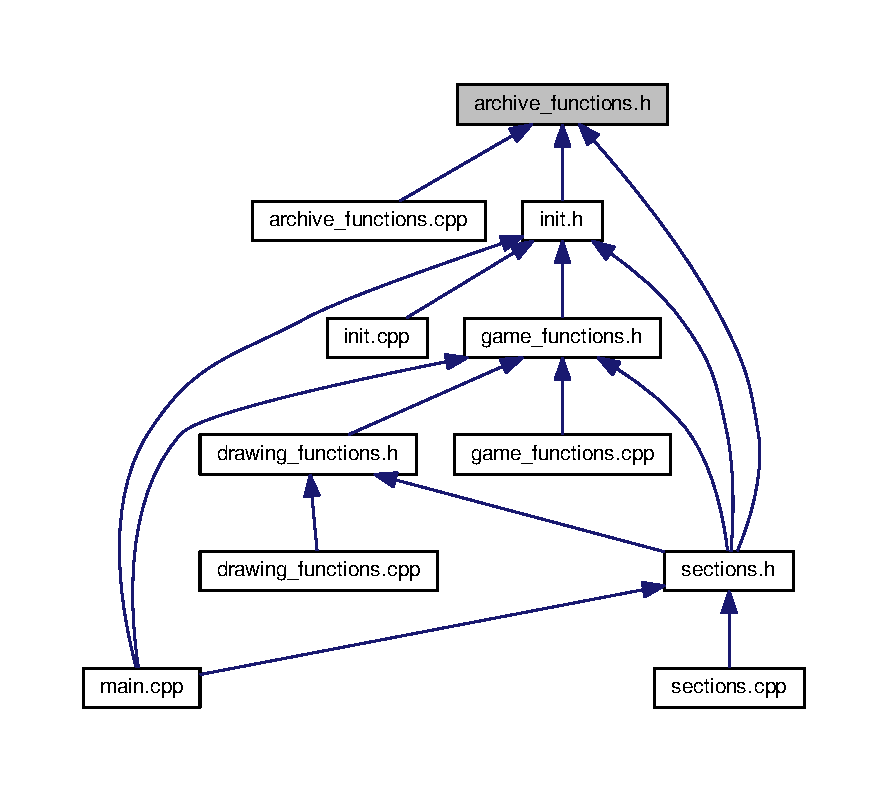
\includegraphics[width=350pt]{db/d22/archive__functions_8h__dep__incl}
\end{center}
\end{figure}
\subsection*{Funzioni}
\begin{DoxyCompactItemize}
\item 
void $\ast$ \hyperlink{archive__functions_8h_a9f84e719a4e4079c5aad042930458381}{start\+\_\+searching} (void $\ast$search\+\_\+manager)
\begin{DoxyCompactList}\small\item\em Funzione che gestire i thread searcher e worker. \end{DoxyCompactList}\end{DoxyCompactItemize}
\subsection*{Variabili}
\begin{DoxyCompactItemize}
\item 
\hyperlink{structthread__manager__t}{thread\+\_\+manager\+\_\+t} \hyperlink{archive__functions_8h_ad04f177b84df22adea5536cbae88451b}{thread\+\_\+manager}
\item 
\hyperlink{structwords__buffer__t}{words\+\_\+buffer\+\_\+t} \hyperlink{archive__functions_8h_aaa25f9883d8c134861353b1bf5e00846}{words\+\_\+buffer}
\end{DoxyCompactItemize}


\subsection{Documentazione delle funzioni}
\mbox{\Hypertarget{archive__functions_8h_a9f84e719a4e4079c5aad042930458381}\label{archive__functions_8h_a9f84e719a4e4079c5aad042930458381}} 
\index{archive\+\_\+functions.\+h@{archive\+\_\+functions.\+h}!start\+\_\+searching@{start\+\_\+searching}}
\index{start\+\_\+searching@{start\+\_\+searching}!archive\+\_\+functions.\+h@{archive\+\_\+functions.\+h}}
\subsubsection{\texorpdfstring{start\+\_\+searching()}{start\_searching()}}
{\footnotesize\ttfamily void$\ast$ start\+\_\+searching (\begin{DoxyParamCaption}\item[{void $\ast$}]{search\+\_\+manager }\end{DoxyParamCaption})}



Funzione che gestire i thread searcher e worker. 

~\newline
Questi thread gestiscono la ricerca dell\textquotesingle{}email dello username all\textquotesingle{}interno delle collection. ~\newline
Parametri\+: ~\newline
1) search\+\_\+manager -\/ Variabile contenente le strutture per la sincronizzazione la ricerca. 

\subsection{Documentazione delle variabili}
\mbox{\Hypertarget{archive__functions_8h_ad04f177b84df22adea5536cbae88451b}\label{archive__functions_8h_ad04f177b84df22adea5536cbae88451b}} 
\index{archive\+\_\+functions.\+h@{archive\+\_\+functions.\+h}!thread\+\_\+manager@{thread\+\_\+manager}}
\index{thread\+\_\+manager@{thread\+\_\+manager}!archive\+\_\+functions.\+h@{archive\+\_\+functions.\+h}}
\subsubsection{\texorpdfstring{thread\+\_\+manager}{thread\_manager}}
{\footnotesize\ttfamily \hyperlink{structthread__manager__t}{thread\+\_\+manager\+\_\+t} thread\+\_\+manager}

\mbox{\Hypertarget{archive__functions_8h_aaa25f9883d8c134861353b1bf5e00846}\label{archive__functions_8h_aaa25f9883d8c134861353b1bf5e00846}} 
\index{archive\+\_\+functions.\+h@{archive\+\_\+functions.\+h}!words\+\_\+buffer@{words\+\_\+buffer}}
\index{words\+\_\+buffer@{words\+\_\+buffer}!archive\+\_\+functions.\+h@{archive\+\_\+functions.\+h}}
\subsubsection{\texorpdfstring{words\+\_\+buffer}{words\_buffer}}
{\footnotesize\ttfamily \hyperlink{structwords__buffer__t}{words\+\_\+buffer\+\_\+t} words\+\_\+buffer}


\hypertarget{data_8h}{}\section{Riferimenti per il file data.\+h}
\label{data_8h}\index{data.\+h@{data.\+h}}
{\ttfamily \#include $<$allegro5/allegro.\+h$>$}\newline
{\ttfamily \#include $<$allegro5/allegro\+\_\+native\+\_\+dialog.\+h$>$}\newline
{\ttfamily \#include $<$allegro5/allegro\+\_\+image.\+h$>$}\newline
{\ttfamily \#include $<$allegro5/allegro\+\_\+primitives.\+h$>$}\newline
{\ttfamily \#include $<$allegro5/allegro\+\_\+font.\+h$>$}\newline
{\ttfamily \#include $<$allegro5/allegro\+\_\+ttf.\+h$>$}\newline
{\ttfamily \#include $<$allegro5/allegro\+\_\+audio.\+h$>$}\newline
{\ttfamily \#include $<$allegro5/allegro\+\_\+acodec.\+h$>$}\newline
{\ttfamily \#include $<$semaphore.\+h$>$}\newline
Grafo delle dipendenze di inclusione per data.\+h\+:\nopagebreak
\begin{figure}[H]
\begin{center}
\leavevmode
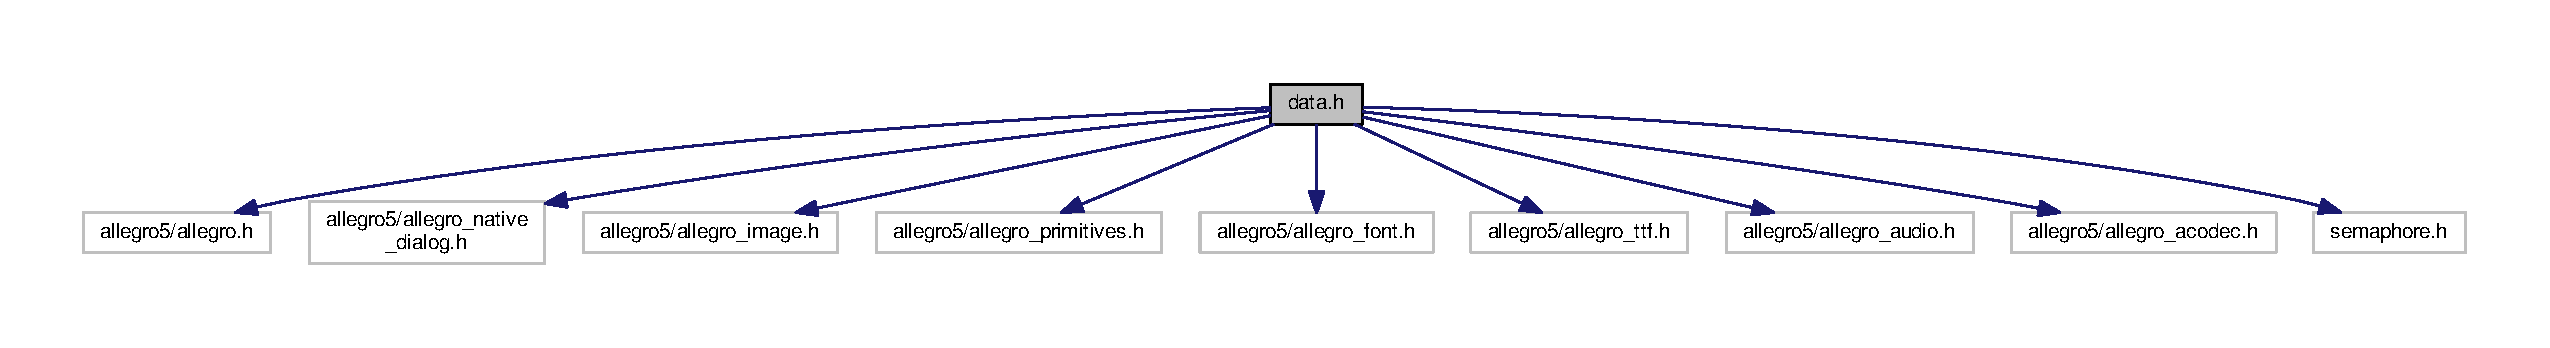
\includegraphics[width=350pt]{d6/d2b/data_8h__incl}
\end{center}
\end{figure}
Questo grafo mostra quali altri file includono direttamente o indirettamente questo file\+:\nopagebreak
\begin{figure}[H]
\begin{center}
\leavevmode
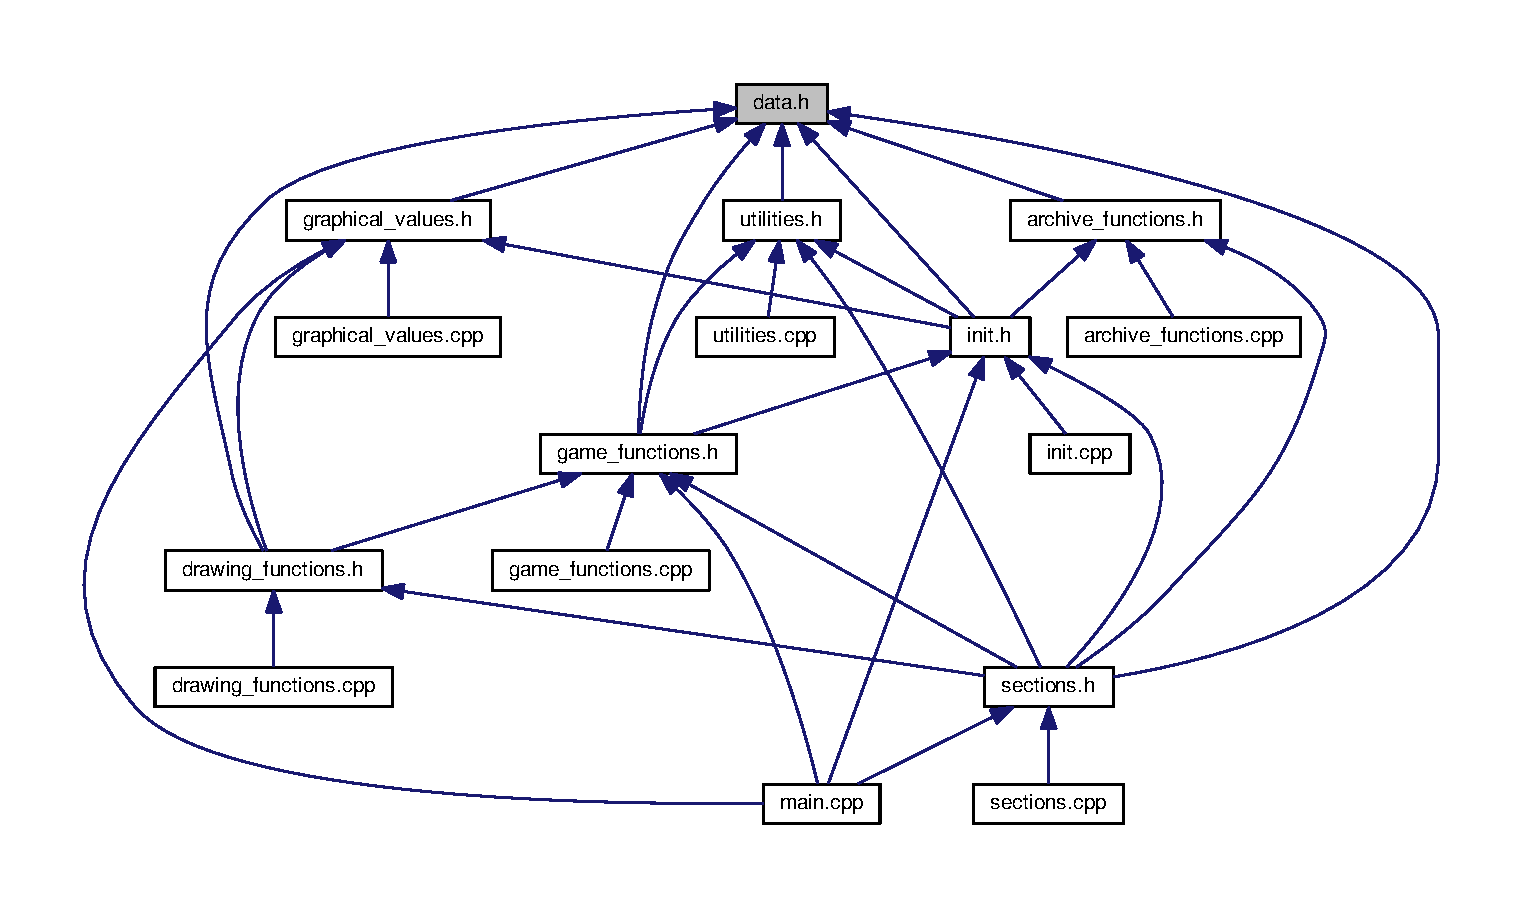
\includegraphics[width=350pt]{d2/d2f/data_8h__dep__incl}
\end{center}
\end{figure}
\subsection*{Composti}
\begin{DoxyCompactItemize}
\item 
struct \hyperlink{structdisplay__info__t}{display\+\_\+info\+\_\+t}
\begin{DoxyCompactList}\small\item\em Struct contenente le informazioni relative al display. \end{DoxyCompactList}\item 
struct \hyperlink{structasteroid__t}{asteroid\+\_\+t}
\begin{DoxyCompactList}\small\item\em Struct contenente le informazioni relative al singolo asteroide. \end{DoxyCompactList}\item 
struct \hyperlink{structelem__asteroid__t}{elem\+\_\+asteroid\+\_\+t}
\begin{DoxyCompactList}\small\item\em Struct del singolo elemento di una lista di asteroidi. \end{DoxyCompactList}\item 
struct \hyperlink{structbullet__t}{bullet\+\_\+t}
\begin{DoxyCompactList}\small\item\em Struct contenente le informazioni relative al singolo proiettile. \end{DoxyCompactList}\item 
struct \hyperlink{structshooter__t}{shooter\+\_\+t}
\begin{DoxyCompactList}\small\item\em Struct contenente le informazioni relative al singolo proiettile. \end{DoxyCompactList}\item 
struct \hyperlink{structresult__t}{result\+\_\+t}
\begin{DoxyCompactList}\small\item\em Struct contenenti le password corrispondenti alla mail data in input dall\textquotesingle{}utente. \end{DoxyCompactList}\item 
struct \hyperlink{structmatch__vars__t}{match\+\_\+vars\+\_\+t}
\begin{DoxyCompactList}\small\item\em Struct contenente le variabili di gioco. \end{DoxyCompactList}\item 
struct \hyperlink{structsettings__t}{settings\+\_\+t}
\begin{DoxyCompactList}\small\item\em Struct contenente le impostazioni di gioco. \end{DoxyCompactList}\item 
struct \hyperlink{structgeneral__gv__t}{general\+\_\+gv\+\_\+t}
\begin{DoxyCompactList}\small\item\em Struct relativo alle proporzioni grafiche generali. \end{DoxyCompactList}\item 
struct \hyperlink{structmenu__gv__t}{menu\+\_\+gv\+\_\+t}
\begin{DoxyCompactList}\small\item\em Struct relativo alle proporzioni grafiche dei menu. \end{DoxyCompactList}\item 
struct \hyperlink{structplaywa__gv__t}{playwa\+\_\+gv\+\_\+t}
\begin{DoxyCompactList}\small\item\em Struct relativo alle proporzioni grafiche della schermata di gioco. \end{DoxyCompactList}\item 
struct \hyperlink{structinstr__gv__t}{instr\+\_\+gv\+\_\+t}
\begin{DoxyCompactList}\small\item\em Struct relativo alle proporzioni grafiche della schermata di pausa. \end{DoxyCompactList}\item 
struct \hyperlink{structusr__gv__t}{usr\+\_\+gv\+\_\+t}
\begin{DoxyCompactList}\small\item\em Struct relativo alle proporzioni grafiche della schermata di fine partita. \end{DoxyCompactList}\item 
struct \hyperlink{structfile__t}{file\+\_\+t}
\begin{DoxyCompactList}\small\item\em Struct relativa alla descrizione di un archivio che andrà esaminato. \end{DoxyCompactList}\item 
struct \hyperlink{structls__t}{ls\+\_\+t}
\begin{DoxyCompactList}\small\item\em Struct che raccoglie tutti gli archivi. \end{DoxyCompactList}\item 
struct \hyperlink{structsearch__manager__t}{search\+\_\+manager\+\_\+t}
\begin{DoxyCompactList}\small\item\em Struct che rappresenta il manager dei thread atti a ricercare le password all\textquotesingle{}interno degli archivi. \end{DoxyCompactList}\item 
struct \hyperlink{structthread__manager__t}{thread\+\_\+manager\+\_\+t}
\begin{DoxyCompactList}\small\item\em Struct che contiene le variabili di sincronizzazione del gioco. \end{DoxyCompactList}\item 
struct \hyperlink{structwords__buffer__t}{words\+\_\+buffer\+\_\+t}
\begin{DoxyCompactList}\small\item\em Struct buffer che implementa l\textquotesingle{}architettura producer/consumer. \end{DoxyCompactList}\item 
struct \hyperlink{structlook__into__t}{look\+\_\+into\+\_\+t}
\begin{DoxyCompactList}\small\item\em Struct di appoggio utilizzata dai thread searcher/worker per ricevere informazioni riguardo\+: 1) filename -\/ dentro quale archivio cercare; 2) email -\/ quale email cercare; 3) is\+\_\+searcher -\/ se il thread si tratta di un searcher (fornisce le parole al gioco) o di un worker. \end{DoxyCompactList}\end{DoxyCompactItemize}
\subsection*{Definizioni}
\begin{DoxyCompactItemize}
\item 
\#define \hyperlink{data_8h_a5e44ee7e5e774b94bc34f1a2e86b3fe6}{T\+I\+M\+E\+R\+\_\+\+S\+H\+I\+E\+L\+D\+\_\+\+B\+O\+N\+US}~8.\+0
\begin{DoxyCompactList}\small\item\em Tempo (in secondi) di durata del bonus \char`\"{}\+Shield\char`\"{}. \end{DoxyCompactList}\item 
\#define \hyperlink{data_8h_a9e0802df8e999c92321e68fcfe300672}{T\+I\+M\+E\+R\+\_\+\+R\+A\+L\+L\+E\+N\+T\+Y\+\_\+\+B\+O\+N\+US}~5.\+0
\begin{DoxyCompactList}\small\item\em Tempo (in secondi) di durata del bonus \char`\"{}\+Rallenty\char`\"{}. \end{DoxyCompactList}\item 
\#define \hyperlink{data_8h_acca7b190290abc33a795032bff506aef}{G\+A\+M\+E\+R\+E\+S\+\_\+W}~1280
\begin{DoxyCompactList}\small\item\em Larghezza della risoluzione base. \end{DoxyCompactList}\item 
\#define \hyperlink{data_8h_ab03f52d3b8949390ea4ecda6c477f410}{G\+A\+M\+E\+R\+E\+S\+\_\+H}~800
\begin{DoxyCompactList}\small\item\em Altezza della risoluzione base. \end{DoxyCompactList}\item 
\#define \hyperlink{data_8h_a8b1f936785c35076c00d66e950d47bd2}{M\+O\+N\+I\+T\+O\+R\+\_\+\+O\+F\+F\+S\+E\+T\+\_\+\+R\+A\+TE}~5
\begin{DoxyCompactList}\small\item\em Frazione di schermo (in altezza) lasciata libera per la creazione della schermata di gioco. \end{DoxyCompactList}\item 
\#define \hyperlink{data_8h_affced4b175e803df59f802e25d017b9b}{N\+U\+M\+\_\+\+I\+T\+E\+MS}~4
\begin{DoxyCompactList}\small\item\em Numerosita\textquotesingle{} dei bonus. \end{DoxyCompactList}\item 
\#define \hyperlink{data_8h_ac32ea00c03c9a9afd1ffc9e1627a8506}{M\+A\+X\+\_\+\+U\+S\+E\+R\+N\+A\+M\+E\+\_\+\+L\+E\+N\+G\+TH}~40
\begin{DoxyCompactList}\small\item\em Lunghezza massima dello username del giocatore. \end{DoxyCompactList}\item 
\#define \hyperlink{data_8h_a3a6cec1114888847d65a0b7a87dd36dd}{M\+A\+X\+\_\+\+A\+S\+T\+E\+R\+O\+I\+D\+\_\+\+H\+E\+AD}~9
\begin{DoxyCompactList}\small\item\em Numero massimo di asteroidi in campo (ovvero in testa alle code). \end{DoxyCompactList}\item 
\#define \hyperlink{data_8h_a9ff4b2e40684ddc4a47b8b02c9fb2afa}{M\+A\+X\+\_\+\+D\+I\+G\+I\+T\+\_\+\+S\+C\+O\+RE}~8
\begin{DoxyCompactList}\small\item\em Numero massimo di caratteri relativi allo score. \end{DoxyCompactList}\item 
\#define \hyperlink{data_8h_aab81d64b66b572b5d81e3f36eac72591}{M\+A\+X\+\_\+\+L\+E\+N\+G\+T\+H\+\_\+\+W\+O\+RD}~8
\begin{DoxyCompactList}\small\item\em Lunghezza massima delle parole che verranno presentate al giocatore. \end{DoxyCompactList}\item 
\#define \hyperlink{data_8h_a88f5ea90744f4c455d0337349a79d723}{M\+A\+X\+\_\+\+M\+A\+T\+C\+H\+I\+N\+G\+\_\+\+P\+A\+SS}~10
\begin{DoxyCompactList}\small\item\em Massimo numero di password cercate negli archivi. \end{DoxyCompactList}\item 
\#define \hyperlink{data_8h_a47b9222ac12a0ba84084dc2690558610}{M\+I\+N\+\_\+\+T\+I\+M\+E\+\_\+\+S\+P\+A\+WN}~0.\+5
\begin{DoxyCompactList}\small\item\em Tempo minimo di spawn tra un asteroide e l\textquotesingle{}altro. \end{DoxyCompactList}\item 
\#define \hyperlink{data_8h_a632dec00f55ca9cb545a41add57e05e2}{N\+U\+M\+\_\+\+M\+E\+N\+U\+\_\+\+B\+I\+T\+M\+A\+PS}~4
\begin{DoxyCompactList}\small\item\em Numero di bitmap relativi ai menu. \end{DoxyCompactList}\item 
\#define \hyperlink{data_8h_ab0ecfd8e12a2e2a1d57e96ddef5fce70}{N\+U\+M\+\_\+\+P\+L\+A\+Y\+W\+A\+\_\+\+B\+I\+T\+M\+A\+PS}~14
\begin{DoxyCompactList}\small\item\em Numero di bitmap relativi alla schermata di gioco. \end{DoxyCompactList}\item 
\#define \hyperlink{data_8h_a7f7b62d0300a1e20185fc33b33bea73a}{N\+U\+M\+\_\+\+I\+N\+S\+T\+R\+\_\+\+B\+I\+T\+M\+A\+PS}~6
\begin{DoxyCompactList}\small\item\em Numero di bitmap relativi alla pausa. \end{DoxyCompactList}\item 
\#define \hyperlink{data_8h_a8d79b09c0b692acd363149b46796cdb5}{N\+U\+M\+\_\+\+M\+E\+N\+U\+\_\+\+F\+O\+N\+TS}~3
\begin{DoxyCompactList}\small\item\em Numero di font relativi ai menu. \end{DoxyCompactList}\item 
\#define \hyperlink{data_8h_adba95d0950cb362ebc8d02b7692587b3}{N\+U\+M\+\_\+\+I\+N\+S\+T\+R\+\_\+\+F\+O\+N\+TS}~4
\begin{DoxyCompactList}\small\item\em Numero di font relativi alla schermata di pausa. \end{DoxyCompactList}\item 
\#define \hyperlink{data_8h_ad9c1911ddd54eba9ce62b51bc6ce6b9f}{N\+U\+M\+\_\+\+S\+E\+T\+T\+I\+N\+G\+S\+\_\+\+F\+O\+N\+TS}~3
\begin{DoxyCompactList}\small\item\em Numero di font relativi al menu delle impostazioni. \end{DoxyCompactList}\item 
\#define \hyperlink{data_8h_afdf4d0cc194ae2d54c40ea5c8799e1de}{N\+U\+M\+\_\+\+P\+L\+A\+Y\+W\+A\+\_\+\+F\+O\+N\+TS}~5
\begin{DoxyCompactList}\small\item\em Numero di font relativi alla schermata di gioco. \end{DoxyCompactList}\item 
\#define \hyperlink{data_8h_af51d343753f0f8c4197593f11c7943f9}{N\+U\+M\+\_\+\+U\+S\+E\+R\+\_\+\+F\+O\+N\+TS}~4
\begin{DoxyCompactList}\small\item\em Numero di font relativi alla schermata di fine partita. \end{DoxyCompactList}\item 
\#define \hyperlink{data_8h_a6c58a590ae37a1cbae1d1b06a85306dd}{B\+G\+\_\+\+R\+E\+F\+R\+E\+S\+H\+\_\+\+T\+I\+ME}~0.\+0005
\begin{DoxyCompactList}\small\item\em Tempo (espresso in secondi) di aggiornamento relativo allo scorrimento dello sfondo. \end{DoxyCompactList}\item 
\#define \hyperlink{data_8h_a7ebeba86e0052d7a48de7828893f4d2b}{N\+U\+M\+\_\+\+O\+P\+T\+I\+O\+NS}~3
\begin{DoxyCompactList}\small\item\em Numero di opzioni presenti nel menu principale. \end{DoxyCompactList}\item 
\#define \hyperlink{data_8h_a9a5f23ce835c1e5895bff9f7186260f8}{N\+U\+M\+\_\+\+O\+P\+T\+I\+O\+N\+S\+\_\+\+S\+E\+T\+T\+I\+N\+GS}~3
\begin{DoxyCompactList}\small\item\em Numero di opzioni presenti nel menu delle impostazioni. \end{DoxyCompactList}\item 
\#define \hyperlink{data_8h_a58f27eafcb451c09c454d20e4ef83edb}{S\+C\+O\+R\+E\+\_\+\+I\+N\+C\+R\+E\+M\+E\+NT}~50
\begin{DoxyCompactList}\small\item\em Punteggio dato dalla distruzione di un asteroide. \end{DoxyCompactList}\item 
\#define \hyperlink{data_8h_a19736b4c86eeb93bb035d5a8623f4e47}{S\+H\+A\+D\+O\+W\+\_\+\+C\+O\+L\+OR}~al\+\_\+map\+\_\+rgba\+\_\+f(0, 0, 0, 0.\+75)
\item 
\#define \hyperlink{data_8h_aba607bb53a6a521c43cdde7ba93fa391}{M\+E\+N\+U\+\_\+\+F\+O\+N\+T\+\_\+\+C\+O\+L\+OR}~al\+\_\+map\+\_\+rgb(246, 242, 212)
\item 
\#define \hyperlink{data_8h_a5b70e07aac9be7838d27b4794af7a07c}{M\+E\+N\+U\+\_\+\+C\+P\+Y\+\_\+\+C\+O\+L\+OR}~al\+\_\+map\+\_\+rgb(122, 124, 119)
\end{DoxyCompactItemize}
\subsection*{Ridefinizioni di tipo (typedef)}
\begin{DoxyCompactItemize}
\item 
typedef \hyperlink{structelem__asteroid__t}{elem\+\_\+asteroid\+\_\+t} $\ast$ \hyperlink{data_8h_a452eef9acfcf76fb85e2c7ecf3b9ff90}{asteroid\+\_\+list}
\begin{DoxyCompactList}\small\item\em Definizione del tipo \char`\"{}lista di asteriodi\char`\"{}. \end{DoxyCompactList}\end{DoxyCompactItemize}
\subsection*{Tipi enumerati (enum)}
\begin{DoxyCompactItemize}
\item 
enum \hyperlink{data_8h_a56839c56ca6deb3cff5e21540ddb8218}{enable\+\_\+t} \{ \hyperlink{data_8h_a56839c56ca6deb3cff5e21540ddb8218a977d478dacaae531f95695750d1e9d03}{ON}, 
\hyperlink{data_8h_a56839c56ca6deb3cff5e21540ddb8218aac132f2982b98bcaa3445e535a03ff75}{O\+FF}
 \}\begin{DoxyCompactList}\small\item\em Enumerato relativo alle impostazioni di gioco\+: attive o non attive. \end{DoxyCompactList}
\item 
enum \hyperlink{data_8h_a07b940e2e86eb4fc3f1e1e1843da0564}{asteroid\+\_\+special\+\_\+t} \{ \newline
\hyperlink{data_8h_a07b940e2e86eb4fc3f1e1e1843da0564a50d1448013c6f17125caee18aa418af7}{N\+O\+R\+M\+AL}, 
\hyperlink{data_8h_a07b940e2e86eb4fc3f1e1e1843da0564ada0b1d3109123d2ec0ef5e8f4fa32262}{A\+T\+O\+M\+IC}, 
\hyperlink{data_8h_a07b940e2e86eb4fc3f1e1e1843da0564a781532b2d0582c3c9c7c3a9d76f0c159}{R\+A\+L\+L\+E\+N\+TY}, 
\hyperlink{data_8h_a07b940e2e86eb4fc3f1e1e1843da0564a6811f08ec3a763b0351fab6fb5054df8}{F\+I\+RE}, 
\newline
\hyperlink{data_8h_a07b940e2e86eb4fc3f1e1e1843da0564affdd98146fb0c71b3381f94b036a100f}{S\+H\+I\+E\+LD}
 \}\begin{DoxyCompactList}\small\item\em Enumerato relativo al bonus contenuto nel singonlo asteroide\+: nessuno, Atomic, Rallenty, Fire o Shield. \end{DoxyCompactList}
\end{DoxyCompactItemize}
\subsection*{Variabili}
\begin{DoxyCompactItemize}
\item 
const int \hyperlink{data_8h_abbb1a97343fdbf54e75f14fb83cb0a92}{N\+\_\+\+Q\+U\+E\+U\+ES} = \textquotesingle{}Z\textquotesingle{} -\/ \textquotesingle{}A\textquotesingle{} + 1
\begin{DoxyCompactList}\small\item\em Numerosita\textquotesingle{} delle code di asteroidi (\textquotesingle{}A\textquotesingle{}..\textquotesingle{}Z\textquotesingle{}) e del buffer. \end{DoxyCompactList}\item 
const char \hyperlink{data_8h_a8b9c6bfbae12c88e6228954f78070560}{M\+U\+S\+I\+C\+\_\+\+M\+E\+N\+U\+\_\+\+P\+A\+T\+H\+\_\+\+WA} \mbox{[}$\,$\mbox{]} = \char`\"{}media/sounds/menu.\+wav\char`\"{}
\begin{DoxyCompactList}\small\item\em Percorso del file audio relativo alla musica dei menu. \end{DoxyCompactList}\item 
const char \hyperlink{data_8h_a8f13920443635ea4f319d0e0842ba280}{M\+U\+S\+I\+C\+\_\+\+G\+A\+M\+E\+O\+V\+E\+R\+\_\+\+P\+A\+T\+H\+\_\+\+WA} \mbox{[}$\,$\mbox{]} = \char`\"{}media/sounds/gameover.\+wav\char`\"{}
\begin{DoxyCompactList}\small\item\em Percorso del file audio relativo alla musica della schermata di gameover. \end{DoxyCompactList}\item 
const char \hyperlink{data_8h_ad18234177a3bd9410ed9837905d071bf}{S\+O\+U\+N\+D\+\_\+\+P\+A\+T\+H\+\_\+\+E\+X\+P\+L\+O\+S\+I\+ON} \mbox{[}$\,$\mbox{]} = \char`\"{}media/sounds/explosion.\+wav\char`\"{}
\begin{DoxyCompactList}\small\item\em Percorso del file audio relativo all\textquotesingle{}effetto sonoro dell\textquotesingle{}esplosione di un asteroide. \end{DoxyCompactList}\item 
const char \hyperlink{data_8h_accf15b03b5957e66ec3a6afa0b26d656}{S\+O\+U\+N\+D\+\_\+\+P\+A\+T\+H\+\_\+\+F\+I\+RE} \mbox{[}$\,$\mbox{]} = \char`\"{}media/sounds/fire.\+wav\char`\"{}
\begin{DoxyCompactList}\small\item\em Percorso del file audio relativo all\textquotesingle{}effetto sonoro dello sparo di un proiettile. \end{DoxyCompactList}\item 
const char \hyperlink{data_8h_a9358d35614f3e5a06b73e2aed0c241db}{S\+O\+U\+N\+D\+\_\+\+P\+A\+T\+H\+\_\+\+E\+R\+R\+OR} \mbox{[}$\,$\mbox{]} = \char`\"{}media/sounds/error.\+wav\char`\"{}
\begin{DoxyCompactList}\small\item\em Percorso del file audio relativo all\textquotesingle{}effetto sonoro che viene riprodotto quando si sbaglia una lettera. \end{DoxyCompactList}\item 
const char \hyperlink{data_8h_ab5aa6954a2f8d619dfc6ebf5ada160a8}{S\+O\+U\+N\+D\+\_\+\+P\+A\+T\+H\+\_\+\+G\+A\+M\+E\+O\+V\+ER} \mbox{[}$\,$\mbox{]} = \char`\"{}media/sounds/death.\+wav\char`\"{}
\begin{DoxyCompactList}\small\item\em Percorso del file audio relativo all\textquotesingle{}effetto sonoro che viene riprodotto quando un asteroide tocca la navicella. \end{DoxyCompactList}\item 
const char \hyperlink{data_8h_a73513865a0c9e121811b8bf52575c71b}{M\+U\+S\+I\+C\+\_\+\+P\+L\+A\+Y\+W\+A\+\_\+\+P\+A\+T\+H\+\_\+\+WA} \mbox{[}$\,$\mbox{]} = \char`\"{}media/sounds/playwa.\+wav\char`\"{}
\begin{DoxyCompactList}\small\item\em Percorso del file audio relativo alla musica della schermata di gioco. \end{DoxyCompactList}\item 
const char \hyperlink{data_8h_a33122e2c233f57480d757de1e6637f23}{F\+O\+N\+T\+\_\+\+P\+A\+TH} \mbox{[}$\,$\mbox{]} = \char`\"{}media/font/visitor.\+ttf\char`\"{}
\begin{DoxyCompactList}\small\item\em Percorso del font utilizzato in tutto il progetto. \end{DoxyCompactList}\item 
const char \hyperlink{data_8h_a00240ac4435599a8c32ffdf40689dab3}{B\+M\+P\+\_\+\+P\+A\+T\+H\+\_\+\+B\+A\+SE} \mbox{[}$\,$\mbox{]} = \char`\"{}media/images/\char`\"{}
\begin{DoxyCompactList}\small\item\em Percorso della cartella contenente le immagini. \end{DoxyCompactList}\end{DoxyCompactItemize}


\subsection{Documentazione delle definizioni}
\mbox{\Hypertarget{data_8h_a6c58a590ae37a1cbae1d1b06a85306dd}\label{data_8h_a6c58a590ae37a1cbae1d1b06a85306dd}} 
\index{data.\+h@{data.\+h}!B\+G\+\_\+\+R\+E\+F\+R\+E\+S\+H\+\_\+\+T\+I\+ME@{B\+G\+\_\+\+R\+E\+F\+R\+E\+S\+H\+\_\+\+T\+I\+ME}}
\index{B\+G\+\_\+\+R\+E\+F\+R\+E\+S\+H\+\_\+\+T\+I\+ME@{B\+G\+\_\+\+R\+E\+F\+R\+E\+S\+H\+\_\+\+T\+I\+ME}!data.\+h@{data.\+h}}
\subsubsection{\texorpdfstring{B\+G\+\_\+\+R\+E\+F\+R\+E\+S\+H\+\_\+\+T\+I\+ME}{BG\_REFRESH\_TIME}}
{\footnotesize\ttfamily \#define B\+G\+\_\+\+R\+E\+F\+R\+E\+S\+H\+\_\+\+T\+I\+ME~0.\+0005}



Tempo (espresso in secondi) di aggiornamento relativo allo scorrimento dello sfondo. 

\mbox{\Hypertarget{data_8h_ab03f52d3b8949390ea4ecda6c477f410}\label{data_8h_ab03f52d3b8949390ea4ecda6c477f410}} 
\index{data.\+h@{data.\+h}!G\+A\+M\+E\+R\+E\+S\+\_\+H@{G\+A\+M\+E\+R\+E\+S\+\_\+H}}
\index{G\+A\+M\+E\+R\+E\+S\+\_\+H@{G\+A\+M\+E\+R\+E\+S\+\_\+H}!data.\+h@{data.\+h}}
\subsubsection{\texorpdfstring{G\+A\+M\+E\+R\+E\+S\+\_\+H}{GAMERES\_H}}
{\footnotesize\ttfamily \#define G\+A\+M\+E\+R\+E\+S\+\_\+H~800}



Altezza della risoluzione base. 

\mbox{\Hypertarget{data_8h_acca7b190290abc33a795032bff506aef}\label{data_8h_acca7b190290abc33a795032bff506aef}} 
\index{data.\+h@{data.\+h}!G\+A\+M\+E\+R\+E\+S\+\_\+W@{G\+A\+M\+E\+R\+E\+S\+\_\+W}}
\index{G\+A\+M\+E\+R\+E\+S\+\_\+W@{G\+A\+M\+E\+R\+E\+S\+\_\+W}!data.\+h@{data.\+h}}
\subsubsection{\texorpdfstring{G\+A\+M\+E\+R\+E\+S\+\_\+W}{GAMERES\_W}}
{\footnotesize\ttfamily \#define G\+A\+M\+E\+R\+E\+S\+\_\+W~1280}



Larghezza della risoluzione base. 

\mbox{\Hypertarget{data_8h_a3a6cec1114888847d65a0b7a87dd36dd}\label{data_8h_a3a6cec1114888847d65a0b7a87dd36dd}} 
\index{data.\+h@{data.\+h}!M\+A\+X\+\_\+\+A\+S\+T\+E\+R\+O\+I\+D\+\_\+\+H\+E\+AD@{M\+A\+X\+\_\+\+A\+S\+T\+E\+R\+O\+I\+D\+\_\+\+H\+E\+AD}}
\index{M\+A\+X\+\_\+\+A\+S\+T\+E\+R\+O\+I\+D\+\_\+\+H\+E\+AD@{M\+A\+X\+\_\+\+A\+S\+T\+E\+R\+O\+I\+D\+\_\+\+H\+E\+AD}!data.\+h@{data.\+h}}
\subsubsection{\texorpdfstring{M\+A\+X\+\_\+\+A\+S\+T\+E\+R\+O\+I\+D\+\_\+\+H\+E\+AD}{MAX\_ASTEROID\_HEAD}}
{\footnotesize\ttfamily \#define M\+A\+X\+\_\+\+A\+S\+T\+E\+R\+O\+I\+D\+\_\+\+H\+E\+AD~9}



Numero massimo di asteroidi in campo (ovvero in testa alle code). 

~\newline
Questo accorgimento garantisce un normale flusso nella generazione degli asteroidi\+: ~\newline
dal momento che le parole relative agli asteroidi vengono generate casualmente, troppe ~\newline
teste occupate (Es. 9 su 10) provocherebbero una situazione di \char`\"{}stallo\char`\"{} dovuto alla ~\newline
probabilità minima di individuare casualmente le teste libere (Es. La decima). \mbox{\Hypertarget{data_8h_a9ff4b2e40684ddc4a47b8b02c9fb2afa}\label{data_8h_a9ff4b2e40684ddc4a47b8b02c9fb2afa}} 
\index{data.\+h@{data.\+h}!M\+A\+X\+\_\+\+D\+I\+G\+I\+T\+\_\+\+S\+C\+O\+RE@{M\+A\+X\+\_\+\+D\+I\+G\+I\+T\+\_\+\+S\+C\+O\+RE}}
\index{M\+A\+X\+\_\+\+D\+I\+G\+I\+T\+\_\+\+S\+C\+O\+RE@{M\+A\+X\+\_\+\+D\+I\+G\+I\+T\+\_\+\+S\+C\+O\+RE}!data.\+h@{data.\+h}}
\subsubsection{\texorpdfstring{M\+A\+X\+\_\+\+D\+I\+G\+I\+T\+\_\+\+S\+C\+O\+RE}{MAX\_DIGIT\_SCORE}}
{\footnotesize\ttfamily \#define M\+A\+X\+\_\+\+D\+I\+G\+I\+T\+\_\+\+S\+C\+O\+RE~8}



Numero massimo di caratteri relativi allo score. 

\mbox{\Hypertarget{data_8h_aab81d64b66b572b5d81e3f36eac72591}\label{data_8h_aab81d64b66b572b5d81e3f36eac72591}} 
\index{data.\+h@{data.\+h}!M\+A\+X\+\_\+\+L\+E\+N\+G\+T\+H\+\_\+\+W\+O\+RD@{M\+A\+X\+\_\+\+L\+E\+N\+G\+T\+H\+\_\+\+W\+O\+RD}}
\index{M\+A\+X\+\_\+\+L\+E\+N\+G\+T\+H\+\_\+\+W\+O\+RD@{M\+A\+X\+\_\+\+L\+E\+N\+G\+T\+H\+\_\+\+W\+O\+RD}!data.\+h@{data.\+h}}
\subsubsection{\texorpdfstring{M\+A\+X\+\_\+\+L\+E\+N\+G\+T\+H\+\_\+\+W\+O\+RD}{MAX\_LENGTH\_WORD}}
{\footnotesize\ttfamily \#define M\+A\+X\+\_\+\+L\+E\+N\+G\+T\+H\+\_\+\+W\+O\+RD~8}



Lunghezza massima delle parole che verranno presentate al giocatore. 

\mbox{\Hypertarget{data_8h_a88f5ea90744f4c455d0337349a79d723}\label{data_8h_a88f5ea90744f4c455d0337349a79d723}} 
\index{data.\+h@{data.\+h}!M\+A\+X\+\_\+\+M\+A\+T\+C\+H\+I\+N\+G\+\_\+\+P\+A\+SS@{M\+A\+X\+\_\+\+M\+A\+T\+C\+H\+I\+N\+G\+\_\+\+P\+A\+SS}}
\index{M\+A\+X\+\_\+\+M\+A\+T\+C\+H\+I\+N\+G\+\_\+\+P\+A\+SS@{M\+A\+X\+\_\+\+M\+A\+T\+C\+H\+I\+N\+G\+\_\+\+P\+A\+SS}!data.\+h@{data.\+h}}
\subsubsection{\texorpdfstring{M\+A\+X\+\_\+\+M\+A\+T\+C\+H\+I\+N\+G\+\_\+\+P\+A\+SS}{MAX\_MATCHING\_PASS}}
{\footnotesize\ttfamily \#define M\+A\+X\+\_\+\+M\+A\+T\+C\+H\+I\+N\+G\+\_\+\+P\+A\+SS~10}



Massimo numero di password cercate negli archivi. 

\mbox{\Hypertarget{data_8h_ac32ea00c03c9a9afd1ffc9e1627a8506}\label{data_8h_ac32ea00c03c9a9afd1ffc9e1627a8506}} 
\index{data.\+h@{data.\+h}!M\+A\+X\+\_\+\+U\+S\+E\+R\+N\+A\+M\+E\+\_\+\+L\+E\+N\+G\+TH@{M\+A\+X\+\_\+\+U\+S\+E\+R\+N\+A\+M\+E\+\_\+\+L\+E\+N\+G\+TH}}
\index{M\+A\+X\+\_\+\+U\+S\+E\+R\+N\+A\+M\+E\+\_\+\+L\+E\+N\+G\+TH@{M\+A\+X\+\_\+\+U\+S\+E\+R\+N\+A\+M\+E\+\_\+\+L\+E\+N\+G\+TH}!data.\+h@{data.\+h}}
\subsubsection{\texorpdfstring{M\+A\+X\+\_\+\+U\+S\+E\+R\+N\+A\+M\+E\+\_\+\+L\+E\+N\+G\+TH}{MAX\_USERNAME\_LENGTH}}
{\footnotesize\ttfamily \#define M\+A\+X\+\_\+\+U\+S\+E\+R\+N\+A\+M\+E\+\_\+\+L\+E\+N\+G\+TH~40}



Lunghezza massima dello username del giocatore. 

\mbox{\Hypertarget{data_8h_a5b70e07aac9be7838d27b4794af7a07c}\label{data_8h_a5b70e07aac9be7838d27b4794af7a07c}} 
\index{data.\+h@{data.\+h}!M\+E\+N\+U\+\_\+\+C\+P\+Y\+\_\+\+C\+O\+L\+OR@{M\+E\+N\+U\+\_\+\+C\+P\+Y\+\_\+\+C\+O\+L\+OR}}
\index{M\+E\+N\+U\+\_\+\+C\+P\+Y\+\_\+\+C\+O\+L\+OR@{M\+E\+N\+U\+\_\+\+C\+P\+Y\+\_\+\+C\+O\+L\+OR}!data.\+h@{data.\+h}}
\subsubsection{\texorpdfstring{M\+E\+N\+U\+\_\+\+C\+P\+Y\+\_\+\+C\+O\+L\+OR}{MENU\_CPY\_COLOR}}
{\footnotesize\ttfamily \#define M\+E\+N\+U\+\_\+\+C\+P\+Y\+\_\+\+C\+O\+L\+OR~al\+\_\+map\+\_\+rgb(122, 124, 119)}

\mbox{\Hypertarget{data_8h_aba607bb53a6a521c43cdde7ba93fa391}\label{data_8h_aba607bb53a6a521c43cdde7ba93fa391}} 
\index{data.\+h@{data.\+h}!M\+E\+N\+U\+\_\+\+F\+O\+N\+T\+\_\+\+C\+O\+L\+OR@{M\+E\+N\+U\+\_\+\+F\+O\+N\+T\+\_\+\+C\+O\+L\+OR}}
\index{M\+E\+N\+U\+\_\+\+F\+O\+N\+T\+\_\+\+C\+O\+L\+OR@{M\+E\+N\+U\+\_\+\+F\+O\+N\+T\+\_\+\+C\+O\+L\+OR}!data.\+h@{data.\+h}}
\subsubsection{\texorpdfstring{M\+E\+N\+U\+\_\+\+F\+O\+N\+T\+\_\+\+C\+O\+L\+OR}{MENU\_FONT\_COLOR}}
{\footnotesize\ttfamily \#define M\+E\+N\+U\+\_\+\+F\+O\+N\+T\+\_\+\+C\+O\+L\+OR~al\+\_\+map\+\_\+rgb(246, 242, 212)}

\mbox{\Hypertarget{data_8h_a47b9222ac12a0ba84084dc2690558610}\label{data_8h_a47b9222ac12a0ba84084dc2690558610}} 
\index{data.\+h@{data.\+h}!M\+I\+N\+\_\+\+T\+I\+M\+E\+\_\+\+S\+P\+A\+WN@{M\+I\+N\+\_\+\+T\+I\+M\+E\+\_\+\+S\+P\+A\+WN}}
\index{M\+I\+N\+\_\+\+T\+I\+M\+E\+\_\+\+S\+P\+A\+WN@{M\+I\+N\+\_\+\+T\+I\+M\+E\+\_\+\+S\+P\+A\+WN}!data.\+h@{data.\+h}}
\subsubsection{\texorpdfstring{M\+I\+N\+\_\+\+T\+I\+M\+E\+\_\+\+S\+P\+A\+WN}{MIN\_TIME\_SPAWN}}
{\footnotesize\ttfamily \#define M\+I\+N\+\_\+\+T\+I\+M\+E\+\_\+\+S\+P\+A\+WN~0.\+5}



Tempo minimo di spawn tra un asteroide e l\textquotesingle{}altro. 

\mbox{\Hypertarget{data_8h_a8b1f936785c35076c00d66e950d47bd2}\label{data_8h_a8b1f936785c35076c00d66e950d47bd2}} 
\index{data.\+h@{data.\+h}!M\+O\+N\+I\+T\+O\+R\+\_\+\+O\+F\+F\+S\+E\+T\+\_\+\+R\+A\+TE@{M\+O\+N\+I\+T\+O\+R\+\_\+\+O\+F\+F\+S\+E\+T\+\_\+\+R\+A\+TE}}
\index{M\+O\+N\+I\+T\+O\+R\+\_\+\+O\+F\+F\+S\+E\+T\+\_\+\+R\+A\+TE@{M\+O\+N\+I\+T\+O\+R\+\_\+\+O\+F\+F\+S\+E\+T\+\_\+\+R\+A\+TE}!data.\+h@{data.\+h}}
\subsubsection{\texorpdfstring{M\+O\+N\+I\+T\+O\+R\+\_\+\+O\+F\+F\+S\+E\+T\+\_\+\+R\+A\+TE}{MONITOR\_OFFSET\_RATE}}
{\footnotesize\ttfamily \#define M\+O\+N\+I\+T\+O\+R\+\_\+\+O\+F\+F\+S\+E\+T\+\_\+\+R\+A\+TE~5}



Frazione di schermo (in altezza) lasciata libera per la creazione della schermata di gioco. 

\mbox{\Hypertarget{data_8h_a7f7b62d0300a1e20185fc33b33bea73a}\label{data_8h_a7f7b62d0300a1e20185fc33b33bea73a}} 
\index{data.\+h@{data.\+h}!N\+U\+M\+\_\+\+I\+N\+S\+T\+R\+\_\+\+B\+I\+T\+M\+A\+PS@{N\+U\+M\+\_\+\+I\+N\+S\+T\+R\+\_\+\+B\+I\+T\+M\+A\+PS}}
\index{N\+U\+M\+\_\+\+I\+N\+S\+T\+R\+\_\+\+B\+I\+T\+M\+A\+PS@{N\+U\+M\+\_\+\+I\+N\+S\+T\+R\+\_\+\+B\+I\+T\+M\+A\+PS}!data.\+h@{data.\+h}}
\subsubsection{\texorpdfstring{N\+U\+M\+\_\+\+I\+N\+S\+T\+R\+\_\+\+B\+I\+T\+M\+A\+PS}{NUM\_INSTR\_BITMAPS}}
{\footnotesize\ttfamily \#define N\+U\+M\+\_\+\+I\+N\+S\+T\+R\+\_\+\+B\+I\+T\+M\+A\+PS~6}



Numero di bitmap relativi alla pausa. 

\mbox{\Hypertarget{data_8h_adba95d0950cb362ebc8d02b7692587b3}\label{data_8h_adba95d0950cb362ebc8d02b7692587b3}} 
\index{data.\+h@{data.\+h}!N\+U\+M\+\_\+\+I\+N\+S\+T\+R\+\_\+\+F\+O\+N\+TS@{N\+U\+M\+\_\+\+I\+N\+S\+T\+R\+\_\+\+F\+O\+N\+TS}}
\index{N\+U\+M\+\_\+\+I\+N\+S\+T\+R\+\_\+\+F\+O\+N\+TS@{N\+U\+M\+\_\+\+I\+N\+S\+T\+R\+\_\+\+F\+O\+N\+TS}!data.\+h@{data.\+h}}
\subsubsection{\texorpdfstring{N\+U\+M\+\_\+\+I\+N\+S\+T\+R\+\_\+\+F\+O\+N\+TS}{NUM\_INSTR\_FONTS}}
{\footnotesize\ttfamily \#define N\+U\+M\+\_\+\+I\+N\+S\+T\+R\+\_\+\+F\+O\+N\+TS~4}



Numero di font relativi alla schermata di pausa. 

\mbox{\Hypertarget{data_8h_affced4b175e803df59f802e25d017b9b}\label{data_8h_affced4b175e803df59f802e25d017b9b}} 
\index{data.\+h@{data.\+h}!N\+U\+M\+\_\+\+I\+T\+E\+MS@{N\+U\+M\+\_\+\+I\+T\+E\+MS}}
\index{N\+U\+M\+\_\+\+I\+T\+E\+MS@{N\+U\+M\+\_\+\+I\+T\+E\+MS}!data.\+h@{data.\+h}}
\subsubsection{\texorpdfstring{N\+U\+M\+\_\+\+I\+T\+E\+MS}{NUM\_ITEMS}}
{\footnotesize\ttfamily \#define N\+U\+M\+\_\+\+I\+T\+E\+MS~4}



Numerosita\textquotesingle{} dei bonus. 

\mbox{\Hypertarget{data_8h_a632dec00f55ca9cb545a41add57e05e2}\label{data_8h_a632dec00f55ca9cb545a41add57e05e2}} 
\index{data.\+h@{data.\+h}!N\+U\+M\+\_\+\+M\+E\+N\+U\+\_\+\+B\+I\+T\+M\+A\+PS@{N\+U\+M\+\_\+\+M\+E\+N\+U\+\_\+\+B\+I\+T\+M\+A\+PS}}
\index{N\+U\+M\+\_\+\+M\+E\+N\+U\+\_\+\+B\+I\+T\+M\+A\+PS@{N\+U\+M\+\_\+\+M\+E\+N\+U\+\_\+\+B\+I\+T\+M\+A\+PS}!data.\+h@{data.\+h}}
\subsubsection{\texorpdfstring{N\+U\+M\+\_\+\+M\+E\+N\+U\+\_\+\+B\+I\+T\+M\+A\+PS}{NUM\_MENU\_BITMAPS}}
{\footnotesize\ttfamily \#define N\+U\+M\+\_\+\+M\+E\+N\+U\+\_\+\+B\+I\+T\+M\+A\+PS~4}



Numero di bitmap relativi ai menu. 

\mbox{\Hypertarget{data_8h_a8d79b09c0b692acd363149b46796cdb5}\label{data_8h_a8d79b09c0b692acd363149b46796cdb5}} 
\index{data.\+h@{data.\+h}!N\+U\+M\+\_\+\+M\+E\+N\+U\+\_\+\+F\+O\+N\+TS@{N\+U\+M\+\_\+\+M\+E\+N\+U\+\_\+\+F\+O\+N\+TS}}
\index{N\+U\+M\+\_\+\+M\+E\+N\+U\+\_\+\+F\+O\+N\+TS@{N\+U\+M\+\_\+\+M\+E\+N\+U\+\_\+\+F\+O\+N\+TS}!data.\+h@{data.\+h}}
\subsubsection{\texorpdfstring{N\+U\+M\+\_\+\+M\+E\+N\+U\+\_\+\+F\+O\+N\+TS}{NUM\_MENU\_FONTS}}
{\footnotesize\ttfamily \#define N\+U\+M\+\_\+\+M\+E\+N\+U\+\_\+\+F\+O\+N\+TS~3}



Numero di font relativi ai menu. 

\mbox{\Hypertarget{data_8h_a7ebeba86e0052d7a48de7828893f4d2b}\label{data_8h_a7ebeba86e0052d7a48de7828893f4d2b}} 
\index{data.\+h@{data.\+h}!N\+U\+M\+\_\+\+O\+P\+T\+I\+O\+NS@{N\+U\+M\+\_\+\+O\+P\+T\+I\+O\+NS}}
\index{N\+U\+M\+\_\+\+O\+P\+T\+I\+O\+NS@{N\+U\+M\+\_\+\+O\+P\+T\+I\+O\+NS}!data.\+h@{data.\+h}}
\subsubsection{\texorpdfstring{N\+U\+M\+\_\+\+O\+P\+T\+I\+O\+NS}{NUM\_OPTIONS}}
{\footnotesize\ttfamily \#define N\+U\+M\+\_\+\+O\+P\+T\+I\+O\+NS~3}



Numero di opzioni presenti nel menu principale. 

\mbox{\Hypertarget{data_8h_a9a5f23ce835c1e5895bff9f7186260f8}\label{data_8h_a9a5f23ce835c1e5895bff9f7186260f8}} 
\index{data.\+h@{data.\+h}!N\+U\+M\+\_\+\+O\+P\+T\+I\+O\+N\+S\+\_\+\+S\+E\+T\+T\+I\+N\+GS@{N\+U\+M\+\_\+\+O\+P\+T\+I\+O\+N\+S\+\_\+\+S\+E\+T\+T\+I\+N\+GS}}
\index{N\+U\+M\+\_\+\+O\+P\+T\+I\+O\+N\+S\+\_\+\+S\+E\+T\+T\+I\+N\+GS@{N\+U\+M\+\_\+\+O\+P\+T\+I\+O\+N\+S\+\_\+\+S\+E\+T\+T\+I\+N\+GS}!data.\+h@{data.\+h}}
\subsubsection{\texorpdfstring{N\+U\+M\+\_\+\+O\+P\+T\+I\+O\+N\+S\+\_\+\+S\+E\+T\+T\+I\+N\+GS}{NUM\_OPTIONS\_SETTINGS}}
{\footnotesize\ttfamily \#define N\+U\+M\+\_\+\+O\+P\+T\+I\+O\+N\+S\+\_\+\+S\+E\+T\+T\+I\+N\+GS~3}



Numero di opzioni presenti nel menu delle impostazioni. 

\mbox{\Hypertarget{data_8h_ab0ecfd8e12a2e2a1d57e96ddef5fce70}\label{data_8h_ab0ecfd8e12a2e2a1d57e96ddef5fce70}} 
\index{data.\+h@{data.\+h}!N\+U\+M\+\_\+\+P\+L\+A\+Y\+W\+A\+\_\+\+B\+I\+T\+M\+A\+PS@{N\+U\+M\+\_\+\+P\+L\+A\+Y\+W\+A\+\_\+\+B\+I\+T\+M\+A\+PS}}
\index{N\+U\+M\+\_\+\+P\+L\+A\+Y\+W\+A\+\_\+\+B\+I\+T\+M\+A\+PS@{N\+U\+M\+\_\+\+P\+L\+A\+Y\+W\+A\+\_\+\+B\+I\+T\+M\+A\+PS}!data.\+h@{data.\+h}}
\subsubsection{\texorpdfstring{N\+U\+M\+\_\+\+P\+L\+A\+Y\+W\+A\+\_\+\+B\+I\+T\+M\+A\+PS}{NUM\_PLAYWA\_BITMAPS}}
{\footnotesize\ttfamily \#define N\+U\+M\+\_\+\+P\+L\+A\+Y\+W\+A\+\_\+\+B\+I\+T\+M\+A\+PS~14}



Numero di bitmap relativi alla schermata di gioco. 

\mbox{\Hypertarget{data_8h_afdf4d0cc194ae2d54c40ea5c8799e1de}\label{data_8h_afdf4d0cc194ae2d54c40ea5c8799e1de}} 
\index{data.\+h@{data.\+h}!N\+U\+M\+\_\+\+P\+L\+A\+Y\+W\+A\+\_\+\+F\+O\+N\+TS@{N\+U\+M\+\_\+\+P\+L\+A\+Y\+W\+A\+\_\+\+F\+O\+N\+TS}}
\index{N\+U\+M\+\_\+\+P\+L\+A\+Y\+W\+A\+\_\+\+F\+O\+N\+TS@{N\+U\+M\+\_\+\+P\+L\+A\+Y\+W\+A\+\_\+\+F\+O\+N\+TS}!data.\+h@{data.\+h}}
\subsubsection{\texorpdfstring{N\+U\+M\+\_\+\+P\+L\+A\+Y\+W\+A\+\_\+\+F\+O\+N\+TS}{NUM\_PLAYWA\_FONTS}}
{\footnotesize\ttfamily \#define N\+U\+M\+\_\+\+P\+L\+A\+Y\+W\+A\+\_\+\+F\+O\+N\+TS~5}



Numero di font relativi alla schermata di gioco. 

\mbox{\Hypertarget{data_8h_ad9c1911ddd54eba9ce62b51bc6ce6b9f}\label{data_8h_ad9c1911ddd54eba9ce62b51bc6ce6b9f}} 
\index{data.\+h@{data.\+h}!N\+U\+M\+\_\+\+S\+E\+T\+T\+I\+N\+G\+S\+\_\+\+F\+O\+N\+TS@{N\+U\+M\+\_\+\+S\+E\+T\+T\+I\+N\+G\+S\+\_\+\+F\+O\+N\+TS}}
\index{N\+U\+M\+\_\+\+S\+E\+T\+T\+I\+N\+G\+S\+\_\+\+F\+O\+N\+TS@{N\+U\+M\+\_\+\+S\+E\+T\+T\+I\+N\+G\+S\+\_\+\+F\+O\+N\+TS}!data.\+h@{data.\+h}}
\subsubsection{\texorpdfstring{N\+U\+M\+\_\+\+S\+E\+T\+T\+I\+N\+G\+S\+\_\+\+F\+O\+N\+TS}{NUM\_SETTINGS\_FONTS}}
{\footnotesize\ttfamily \#define N\+U\+M\+\_\+\+S\+E\+T\+T\+I\+N\+G\+S\+\_\+\+F\+O\+N\+TS~3}



Numero di font relativi al menu delle impostazioni. 

\mbox{\Hypertarget{data_8h_af51d343753f0f8c4197593f11c7943f9}\label{data_8h_af51d343753f0f8c4197593f11c7943f9}} 
\index{data.\+h@{data.\+h}!N\+U\+M\+\_\+\+U\+S\+E\+R\+\_\+\+F\+O\+N\+TS@{N\+U\+M\+\_\+\+U\+S\+E\+R\+\_\+\+F\+O\+N\+TS}}
\index{N\+U\+M\+\_\+\+U\+S\+E\+R\+\_\+\+F\+O\+N\+TS@{N\+U\+M\+\_\+\+U\+S\+E\+R\+\_\+\+F\+O\+N\+TS}!data.\+h@{data.\+h}}
\subsubsection{\texorpdfstring{N\+U\+M\+\_\+\+U\+S\+E\+R\+\_\+\+F\+O\+N\+TS}{NUM\_USER\_FONTS}}
{\footnotesize\ttfamily \#define N\+U\+M\+\_\+\+U\+S\+E\+R\+\_\+\+F\+O\+N\+TS~4}



Numero di font relativi alla schermata di fine partita. 

\mbox{\Hypertarget{data_8h_a58f27eafcb451c09c454d20e4ef83edb}\label{data_8h_a58f27eafcb451c09c454d20e4ef83edb}} 
\index{data.\+h@{data.\+h}!S\+C\+O\+R\+E\+\_\+\+I\+N\+C\+R\+E\+M\+E\+NT@{S\+C\+O\+R\+E\+\_\+\+I\+N\+C\+R\+E\+M\+E\+NT}}
\index{S\+C\+O\+R\+E\+\_\+\+I\+N\+C\+R\+E\+M\+E\+NT@{S\+C\+O\+R\+E\+\_\+\+I\+N\+C\+R\+E\+M\+E\+NT}!data.\+h@{data.\+h}}
\subsubsection{\texorpdfstring{S\+C\+O\+R\+E\+\_\+\+I\+N\+C\+R\+E\+M\+E\+NT}{SCORE\_INCREMENT}}
{\footnotesize\ttfamily \#define S\+C\+O\+R\+E\+\_\+\+I\+N\+C\+R\+E\+M\+E\+NT~50}



Punteggio dato dalla distruzione di un asteroide. 

\mbox{\Hypertarget{data_8h_a19736b4c86eeb93bb035d5a8623f4e47}\label{data_8h_a19736b4c86eeb93bb035d5a8623f4e47}} 
\index{data.\+h@{data.\+h}!S\+H\+A\+D\+O\+W\+\_\+\+C\+O\+L\+OR@{S\+H\+A\+D\+O\+W\+\_\+\+C\+O\+L\+OR}}
\index{S\+H\+A\+D\+O\+W\+\_\+\+C\+O\+L\+OR@{S\+H\+A\+D\+O\+W\+\_\+\+C\+O\+L\+OR}!data.\+h@{data.\+h}}
\subsubsection{\texorpdfstring{S\+H\+A\+D\+O\+W\+\_\+\+C\+O\+L\+OR}{SHADOW\_COLOR}}
{\footnotesize\ttfamily \#define S\+H\+A\+D\+O\+W\+\_\+\+C\+O\+L\+OR~al\+\_\+map\+\_\+rgba\+\_\+f(0, 0, 0, 0.\+75)}

\mbox{\Hypertarget{data_8h_a9e0802df8e999c92321e68fcfe300672}\label{data_8h_a9e0802df8e999c92321e68fcfe300672}} 
\index{data.\+h@{data.\+h}!T\+I\+M\+E\+R\+\_\+\+R\+A\+L\+L\+E\+N\+T\+Y\+\_\+\+B\+O\+N\+US@{T\+I\+M\+E\+R\+\_\+\+R\+A\+L\+L\+E\+N\+T\+Y\+\_\+\+B\+O\+N\+US}}
\index{T\+I\+M\+E\+R\+\_\+\+R\+A\+L\+L\+E\+N\+T\+Y\+\_\+\+B\+O\+N\+US@{T\+I\+M\+E\+R\+\_\+\+R\+A\+L\+L\+E\+N\+T\+Y\+\_\+\+B\+O\+N\+US}!data.\+h@{data.\+h}}
\subsubsection{\texorpdfstring{T\+I\+M\+E\+R\+\_\+\+R\+A\+L\+L\+E\+N\+T\+Y\+\_\+\+B\+O\+N\+US}{TIMER\_RALLENTY\_BONUS}}
{\footnotesize\ttfamily \#define T\+I\+M\+E\+R\+\_\+\+R\+A\+L\+L\+E\+N\+T\+Y\+\_\+\+B\+O\+N\+US~5.\+0}



Tempo (in secondi) di durata del bonus \char`\"{}\+Rallenty\char`\"{}. 

\mbox{\Hypertarget{data_8h_a5e44ee7e5e774b94bc34f1a2e86b3fe6}\label{data_8h_a5e44ee7e5e774b94bc34f1a2e86b3fe6}} 
\index{data.\+h@{data.\+h}!T\+I\+M\+E\+R\+\_\+\+S\+H\+I\+E\+L\+D\+\_\+\+B\+O\+N\+US@{T\+I\+M\+E\+R\+\_\+\+S\+H\+I\+E\+L\+D\+\_\+\+B\+O\+N\+US}}
\index{T\+I\+M\+E\+R\+\_\+\+S\+H\+I\+E\+L\+D\+\_\+\+B\+O\+N\+US@{T\+I\+M\+E\+R\+\_\+\+S\+H\+I\+E\+L\+D\+\_\+\+B\+O\+N\+US}!data.\+h@{data.\+h}}
\subsubsection{\texorpdfstring{T\+I\+M\+E\+R\+\_\+\+S\+H\+I\+E\+L\+D\+\_\+\+B\+O\+N\+US}{TIMER\_SHIELD\_BONUS}}
{\footnotesize\ttfamily \#define T\+I\+M\+E\+R\+\_\+\+S\+H\+I\+E\+L\+D\+\_\+\+B\+O\+N\+US~8.\+0}



Tempo (in secondi) di durata del bonus \char`\"{}\+Shield\char`\"{}. 



\subsection{Documentazione delle ridefinizioni di tipo (typedef)}
\mbox{\Hypertarget{data_8h_a452eef9acfcf76fb85e2c7ecf3b9ff90}\label{data_8h_a452eef9acfcf76fb85e2c7ecf3b9ff90}} 
\index{data.\+h@{data.\+h}!asteroid\+\_\+list@{asteroid\+\_\+list}}
\index{asteroid\+\_\+list@{asteroid\+\_\+list}!data.\+h@{data.\+h}}
\subsubsection{\texorpdfstring{asteroid\+\_\+list}{asteroid\_list}}
{\footnotesize\ttfamily typedef \hyperlink{structelem__asteroid__t}{elem\+\_\+asteroid\+\_\+t}$\ast$ \hyperlink{data_8h_a452eef9acfcf76fb85e2c7ecf3b9ff90}{asteroid\+\_\+list}}



Definizione del tipo \char`\"{}lista di asteriodi\char`\"{}. 



\subsection{Documentazione dei tipi enumerati}
\mbox{\Hypertarget{data_8h_a07b940e2e86eb4fc3f1e1e1843da0564}\label{data_8h_a07b940e2e86eb4fc3f1e1e1843da0564}} 
\index{data.\+h@{data.\+h}!asteroid\+\_\+special\+\_\+t@{asteroid\+\_\+special\+\_\+t}}
\index{asteroid\+\_\+special\+\_\+t@{asteroid\+\_\+special\+\_\+t}!data.\+h@{data.\+h}}
\subsubsection{\texorpdfstring{asteroid\+\_\+special\+\_\+t}{asteroid\_special\_t}}
{\footnotesize\ttfamily enum \hyperlink{data_8h_a07b940e2e86eb4fc3f1e1e1843da0564}{asteroid\+\_\+special\+\_\+t}}



Enumerato relativo al bonus contenuto nel singonlo asteroide\+: nessuno, Atomic, Rallenty, Fire o Shield. 

\begin{DoxyEnumFields}{Valori del tipo enumerato}
\raisebox{\heightof{T}}[0pt][0pt]{\index{N\+O\+R\+M\+AL@{N\+O\+R\+M\+AL}!data.\+h@{data.\+h}}\index{data.\+h@{data.\+h}!N\+O\+R\+M\+AL@{N\+O\+R\+M\+AL}}}\mbox{\Hypertarget{data_8h_a07b940e2e86eb4fc3f1e1e1843da0564a50d1448013c6f17125caee18aa418af7}\label{data_8h_a07b940e2e86eb4fc3f1e1e1843da0564a50d1448013c6f17125caee18aa418af7}} 
N\+O\+R\+M\+AL&\\
\hline

\raisebox{\heightof{T}}[0pt][0pt]{\index{A\+T\+O\+M\+IC@{A\+T\+O\+M\+IC}!data.\+h@{data.\+h}}\index{data.\+h@{data.\+h}!A\+T\+O\+M\+IC@{A\+T\+O\+M\+IC}}}\mbox{\Hypertarget{data_8h_a07b940e2e86eb4fc3f1e1e1843da0564ada0b1d3109123d2ec0ef5e8f4fa32262}\label{data_8h_a07b940e2e86eb4fc3f1e1e1843da0564ada0b1d3109123d2ec0ef5e8f4fa32262}} 
A\+T\+O\+M\+IC&\\
\hline

\raisebox{\heightof{T}}[0pt][0pt]{\index{R\+A\+L\+L\+E\+N\+TY@{R\+A\+L\+L\+E\+N\+TY}!data.\+h@{data.\+h}}\index{data.\+h@{data.\+h}!R\+A\+L\+L\+E\+N\+TY@{R\+A\+L\+L\+E\+N\+TY}}}\mbox{\Hypertarget{data_8h_a07b940e2e86eb4fc3f1e1e1843da0564a781532b2d0582c3c9c7c3a9d76f0c159}\label{data_8h_a07b940e2e86eb4fc3f1e1e1843da0564a781532b2d0582c3c9c7c3a9d76f0c159}} 
R\+A\+L\+L\+E\+N\+TY&\\
\hline

\raisebox{\heightof{T}}[0pt][0pt]{\index{F\+I\+RE@{F\+I\+RE}!data.\+h@{data.\+h}}\index{data.\+h@{data.\+h}!F\+I\+RE@{F\+I\+RE}}}\mbox{\Hypertarget{data_8h_a07b940e2e86eb4fc3f1e1e1843da0564a6811f08ec3a763b0351fab6fb5054df8}\label{data_8h_a07b940e2e86eb4fc3f1e1e1843da0564a6811f08ec3a763b0351fab6fb5054df8}} 
F\+I\+RE&\\
\hline

\raisebox{\heightof{T}}[0pt][0pt]{\index{S\+H\+I\+E\+LD@{S\+H\+I\+E\+LD}!data.\+h@{data.\+h}}\index{data.\+h@{data.\+h}!S\+H\+I\+E\+LD@{S\+H\+I\+E\+LD}}}\mbox{\Hypertarget{data_8h_a07b940e2e86eb4fc3f1e1e1843da0564affdd98146fb0c71b3381f94b036a100f}\label{data_8h_a07b940e2e86eb4fc3f1e1e1843da0564affdd98146fb0c71b3381f94b036a100f}} 
S\+H\+I\+E\+LD&\\
\hline

\end{DoxyEnumFields}
\mbox{\Hypertarget{data_8h_a56839c56ca6deb3cff5e21540ddb8218}\label{data_8h_a56839c56ca6deb3cff5e21540ddb8218}} 
\index{data.\+h@{data.\+h}!enable\+\_\+t@{enable\+\_\+t}}
\index{enable\+\_\+t@{enable\+\_\+t}!data.\+h@{data.\+h}}
\subsubsection{\texorpdfstring{enable\+\_\+t}{enable\_t}}
{\footnotesize\ttfamily enum \hyperlink{data_8h_a56839c56ca6deb3cff5e21540ddb8218}{enable\+\_\+t}}



Enumerato relativo alle impostazioni di gioco\+: attive o non attive. 

\begin{DoxyEnumFields}{Valori del tipo enumerato}
\raisebox{\heightof{T}}[0pt][0pt]{\index{ON@{ON}!data.\+h@{data.\+h}}\index{data.\+h@{data.\+h}!ON@{ON}}}\mbox{\Hypertarget{data_8h_a56839c56ca6deb3cff5e21540ddb8218a977d478dacaae531f95695750d1e9d03}\label{data_8h_a56839c56ca6deb3cff5e21540ddb8218a977d478dacaae531f95695750d1e9d03}} 
ON&\\
\hline

\raisebox{\heightof{T}}[0pt][0pt]{\index{O\+FF@{O\+FF}!data.\+h@{data.\+h}}\index{data.\+h@{data.\+h}!O\+FF@{O\+FF}}}\mbox{\Hypertarget{data_8h_a56839c56ca6deb3cff5e21540ddb8218aac132f2982b98bcaa3445e535a03ff75}\label{data_8h_a56839c56ca6deb3cff5e21540ddb8218aac132f2982b98bcaa3445e535a03ff75}} 
O\+FF&\\
\hline

\end{DoxyEnumFields}


\subsection{Documentazione delle variabili}
\mbox{\Hypertarget{data_8h_a00240ac4435599a8c32ffdf40689dab3}\label{data_8h_a00240ac4435599a8c32ffdf40689dab3}} 
\index{data.\+h@{data.\+h}!B\+M\+P\+\_\+\+P\+A\+T\+H\+\_\+\+B\+A\+SE@{B\+M\+P\+\_\+\+P\+A\+T\+H\+\_\+\+B\+A\+SE}}
\index{B\+M\+P\+\_\+\+P\+A\+T\+H\+\_\+\+B\+A\+SE@{B\+M\+P\+\_\+\+P\+A\+T\+H\+\_\+\+B\+A\+SE}!data.\+h@{data.\+h}}
\subsubsection{\texorpdfstring{B\+M\+P\+\_\+\+P\+A\+T\+H\+\_\+\+B\+A\+SE}{BMP\_PATH\_BASE}}
{\footnotesize\ttfamily const char B\+M\+P\+\_\+\+P\+A\+T\+H\+\_\+\+B\+A\+SE\mbox{[}$\,$\mbox{]} = \char`\"{}media/images/\char`\"{}}



Percorso della cartella contenente le immagini. 

\mbox{\Hypertarget{data_8h_a33122e2c233f57480d757de1e6637f23}\label{data_8h_a33122e2c233f57480d757de1e6637f23}} 
\index{data.\+h@{data.\+h}!F\+O\+N\+T\+\_\+\+P\+A\+TH@{F\+O\+N\+T\+\_\+\+P\+A\+TH}}
\index{F\+O\+N\+T\+\_\+\+P\+A\+TH@{F\+O\+N\+T\+\_\+\+P\+A\+TH}!data.\+h@{data.\+h}}
\subsubsection{\texorpdfstring{F\+O\+N\+T\+\_\+\+P\+A\+TH}{FONT\_PATH}}
{\footnotesize\ttfamily const char F\+O\+N\+T\+\_\+\+P\+A\+TH\mbox{[}$\,$\mbox{]} = \char`\"{}media/font/visitor.\+ttf\char`\"{}}



Percorso del font utilizzato in tutto il progetto. 

\mbox{\Hypertarget{data_8h_a8f13920443635ea4f319d0e0842ba280}\label{data_8h_a8f13920443635ea4f319d0e0842ba280}} 
\index{data.\+h@{data.\+h}!M\+U\+S\+I\+C\+\_\+\+G\+A\+M\+E\+O\+V\+E\+R\+\_\+\+P\+A\+T\+H\+\_\+\+WA@{M\+U\+S\+I\+C\+\_\+\+G\+A\+M\+E\+O\+V\+E\+R\+\_\+\+P\+A\+T\+H\+\_\+\+WA}}
\index{M\+U\+S\+I\+C\+\_\+\+G\+A\+M\+E\+O\+V\+E\+R\+\_\+\+P\+A\+T\+H\+\_\+\+WA@{M\+U\+S\+I\+C\+\_\+\+G\+A\+M\+E\+O\+V\+E\+R\+\_\+\+P\+A\+T\+H\+\_\+\+WA}!data.\+h@{data.\+h}}
\subsubsection{\texorpdfstring{M\+U\+S\+I\+C\+\_\+\+G\+A\+M\+E\+O\+V\+E\+R\+\_\+\+P\+A\+T\+H\+\_\+\+WA}{MUSIC\_GAMEOVER\_PATH\_WA}}
{\footnotesize\ttfamily const char M\+U\+S\+I\+C\+\_\+\+G\+A\+M\+E\+O\+V\+E\+R\+\_\+\+P\+A\+T\+H\+\_\+\+WA\mbox{[}$\,$\mbox{]} = \char`\"{}media/sounds/gameover.\+wav\char`\"{}}



Percorso del file audio relativo alla musica della schermata di gameover. 

\mbox{\Hypertarget{data_8h_a8b9c6bfbae12c88e6228954f78070560}\label{data_8h_a8b9c6bfbae12c88e6228954f78070560}} 
\index{data.\+h@{data.\+h}!M\+U\+S\+I\+C\+\_\+\+M\+E\+N\+U\+\_\+\+P\+A\+T\+H\+\_\+\+WA@{M\+U\+S\+I\+C\+\_\+\+M\+E\+N\+U\+\_\+\+P\+A\+T\+H\+\_\+\+WA}}
\index{M\+U\+S\+I\+C\+\_\+\+M\+E\+N\+U\+\_\+\+P\+A\+T\+H\+\_\+\+WA@{M\+U\+S\+I\+C\+\_\+\+M\+E\+N\+U\+\_\+\+P\+A\+T\+H\+\_\+\+WA}!data.\+h@{data.\+h}}
\subsubsection{\texorpdfstring{M\+U\+S\+I\+C\+\_\+\+M\+E\+N\+U\+\_\+\+P\+A\+T\+H\+\_\+\+WA}{MUSIC\_MENU\_PATH\_WA}}
{\footnotesize\ttfamily const char M\+U\+S\+I\+C\+\_\+\+M\+E\+N\+U\+\_\+\+P\+A\+T\+H\+\_\+\+WA\mbox{[}$\,$\mbox{]} = \char`\"{}media/sounds/menu.\+wav\char`\"{}}



Percorso del file audio relativo alla musica dei menu. 

\mbox{\Hypertarget{data_8h_a73513865a0c9e121811b8bf52575c71b}\label{data_8h_a73513865a0c9e121811b8bf52575c71b}} 
\index{data.\+h@{data.\+h}!M\+U\+S\+I\+C\+\_\+\+P\+L\+A\+Y\+W\+A\+\_\+\+P\+A\+T\+H\+\_\+\+WA@{M\+U\+S\+I\+C\+\_\+\+P\+L\+A\+Y\+W\+A\+\_\+\+P\+A\+T\+H\+\_\+\+WA}}
\index{M\+U\+S\+I\+C\+\_\+\+P\+L\+A\+Y\+W\+A\+\_\+\+P\+A\+T\+H\+\_\+\+WA@{M\+U\+S\+I\+C\+\_\+\+P\+L\+A\+Y\+W\+A\+\_\+\+P\+A\+T\+H\+\_\+\+WA}!data.\+h@{data.\+h}}
\subsubsection{\texorpdfstring{M\+U\+S\+I\+C\+\_\+\+P\+L\+A\+Y\+W\+A\+\_\+\+P\+A\+T\+H\+\_\+\+WA}{MUSIC\_PLAYWA\_PATH\_WA}}
{\footnotesize\ttfamily const char M\+U\+S\+I\+C\+\_\+\+P\+L\+A\+Y\+W\+A\+\_\+\+P\+A\+T\+H\+\_\+\+WA\mbox{[}$\,$\mbox{]} = \char`\"{}media/sounds/playwa.\+wav\char`\"{}}



Percorso del file audio relativo alla musica della schermata di gioco. 

\mbox{\Hypertarget{data_8h_abbb1a97343fdbf54e75f14fb83cb0a92}\label{data_8h_abbb1a97343fdbf54e75f14fb83cb0a92}} 
\index{data.\+h@{data.\+h}!N\+\_\+\+Q\+U\+E\+U\+ES@{N\+\_\+\+Q\+U\+E\+U\+ES}}
\index{N\+\_\+\+Q\+U\+E\+U\+ES@{N\+\_\+\+Q\+U\+E\+U\+ES}!data.\+h@{data.\+h}}
\subsubsection{\texorpdfstring{N\+\_\+\+Q\+U\+E\+U\+ES}{N\_QUEUES}}
{\footnotesize\ttfamily const int N\+\_\+\+Q\+U\+E\+U\+ES = \textquotesingle{}Z\textquotesingle{} -\/ \textquotesingle{}A\textquotesingle{} + 1}



Numerosita\textquotesingle{} delle code di asteroidi (\textquotesingle{}A\textquotesingle{}..\textquotesingle{}Z\textquotesingle{}) e del buffer. 

\mbox{\Hypertarget{data_8h_a9358d35614f3e5a06b73e2aed0c241db}\label{data_8h_a9358d35614f3e5a06b73e2aed0c241db}} 
\index{data.\+h@{data.\+h}!S\+O\+U\+N\+D\+\_\+\+P\+A\+T\+H\+\_\+\+E\+R\+R\+OR@{S\+O\+U\+N\+D\+\_\+\+P\+A\+T\+H\+\_\+\+E\+R\+R\+OR}}
\index{S\+O\+U\+N\+D\+\_\+\+P\+A\+T\+H\+\_\+\+E\+R\+R\+OR@{S\+O\+U\+N\+D\+\_\+\+P\+A\+T\+H\+\_\+\+E\+R\+R\+OR}!data.\+h@{data.\+h}}
\subsubsection{\texorpdfstring{S\+O\+U\+N\+D\+\_\+\+P\+A\+T\+H\+\_\+\+E\+R\+R\+OR}{SOUND\_PATH\_ERROR}}
{\footnotesize\ttfamily const char S\+O\+U\+N\+D\+\_\+\+P\+A\+T\+H\+\_\+\+E\+R\+R\+OR\mbox{[}$\,$\mbox{]} = \char`\"{}media/sounds/error.\+wav\char`\"{}}



Percorso del file audio relativo all\textquotesingle{}effetto sonoro che viene riprodotto quando si sbaglia una lettera. 

\mbox{\Hypertarget{data_8h_ad18234177a3bd9410ed9837905d071bf}\label{data_8h_ad18234177a3bd9410ed9837905d071bf}} 
\index{data.\+h@{data.\+h}!S\+O\+U\+N\+D\+\_\+\+P\+A\+T\+H\+\_\+\+E\+X\+P\+L\+O\+S\+I\+ON@{S\+O\+U\+N\+D\+\_\+\+P\+A\+T\+H\+\_\+\+E\+X\+P\+L\+O\+S\+I\+ON}}
\index{S\+O\+U\+N\+D\+\_\+\+P\+A\+T\+H\+\_\+\+E\+X\+P\+L\+O\+S\+I\+ON@{S\+O\+U\+N\+D\+\_\+\+P\+A\+T\+H\+\_\+\+E\+X\+P\+L\+O\+S\+I\+ON}!data.\+h@{data.\+h}}
\subsubsection{\texorpdfstring{S\+O\+U\+N\+D\+\_\+\+P\+A\+T\+H\+\_\+\+E\+X\+P\+L\+O\+S\+I\+ON}{SOUND\_PATH\_EXPLOSION}}
{\footnotesize\ttfamily const char S\+O\+U\+N\+D\+\_\+\+P\+A\+T\+H\+\_\+\+E\+X\+P\+L\+O\+S\+I\+ON\mbox{[}$\,$\mbox{]} = \char`\"{}media/sounds/explosion.\+wav\char`\"{}}



Percorso del file audio relativo all\textquotesingle{}effetto sonoro dell\textquotesingle{}esplosione di un asteroide. 

\mbox{\Hypertarget{data_8h_accf15b03b5957e66ec3a6afa0b26d656}\label{data_8h_accf15b03b5957e66ec3a6afa0b26d656}} 
\index{data.\+h@{data.\+h}!S\+O\+U\+N\+D\+\_\+\+P\+A\+T\+H\+\_\+\+F\+I\+RE@{S\+O\+U\+N\+D\+\_\+\+P\+A\+T\+H\+\_\+\+F\+I\+RE}}
\index{S\+O\+U\+N\+D\+\_\+\+P\+A\+T\+H\+\_\+\+F\+I\+RE@{S\+O\+U\+N\+D\+\_\+\+P\+A\+T\+H\+\_\+\+F\+I\+RE}!data.\+h@{data.\+h}}
\subsubsection{\texorpdfstring{S\+O\+U\+N\+D\+\_\+\+P\+A\+T\+H\+\_\+\+F\+I\+RE}{SOUND\_PATH\_FIRE}}
{\footnotesize\ttfamily const char S\+O\+U\+N\+D\+\_\+\+P\+A\+T\+H\+\_\+\+F\+I\+RE\mbox{[}$\,$\mbox{]} = \char`\"{}media/sounds/fire.\+wav\char`\"{}}



Percorso del file audio relativo all\textquotesingle{}effetto sonoro dello sparo di un proiettile. 

\mbox{\Hypertarget{data_8h_ab5aa6954a2f8d619dfc6ebf5ada160a8}\label{data_8h_ab5aa6954a2f8d619dfc6ebf5ada160a8}} 
\index{data.\+h@{data.\+h}!S\+O\+U\+N\+D\+\_\+\+P\+A\+T\+H\+\_\+\+G\+A\+M\+E\+O\+V\+ER@{S\+O\+U\+N\+D\+\_\+\+P\+A\+T\+H\+\_\+\+G\+A\+M\+E\+O\+V\+ER}}
\index{S\+O\+U\+N\+D\+\_\+\+P\+A\+T\+H\+\_\+\+G\+A\+M\+E\+O\+V\+ER@{S\+O\+U\+N\+D\+\_\+\+P\+A\+T\+H\+\_\+\+G\+A\+M\+E\+O\+V\+ER}!data.\+h@{data.\+h}}
\subsubsection{\texorpdfstring{S\+O\+U\+N\+D\+\_\+\+P\+A\+T\+H\+\_\+\+G\+A\+M\+E\+O\+V\+ER}{SOUND\_PATH\_GAMEOVER}}
{\footnotesize\ttfamily const char S\+O\+U\+N\+D\+\_\+\+P\+A\+T\+H\+\_\+\+G\+A\+M\+E\+O\+V\+ER\mbox{[}$\,$\mbox{]} = \char`\"{}media/sounds/death.\+wav\char`\"{}}



Percorso del file audio relativo all\textquotesingle{}effetto sonoro che viene riprodotto quando un asteroide tocca la navicella. 


\hypertarget{drawing__functions_8cpp}{}\section{Riferimenti per il file drawing\+\_\+functions.\+cpp}
\label{drawing__functions_8cpp}\index{drawing\+\_\+functions.\+cpp@{drawing\+\_\+functions.\+cpp}}
{\ttfamily \#include \char`\"{}drawing\+\_\+functions.\+h\char`\"{}}\newline
Grafo delle dipendenze di inclusione per drawing\+\_\+functions.\+cpp\+:\nopagebreak
\begin{figure}[H]
\begin{center}
\leavevmode
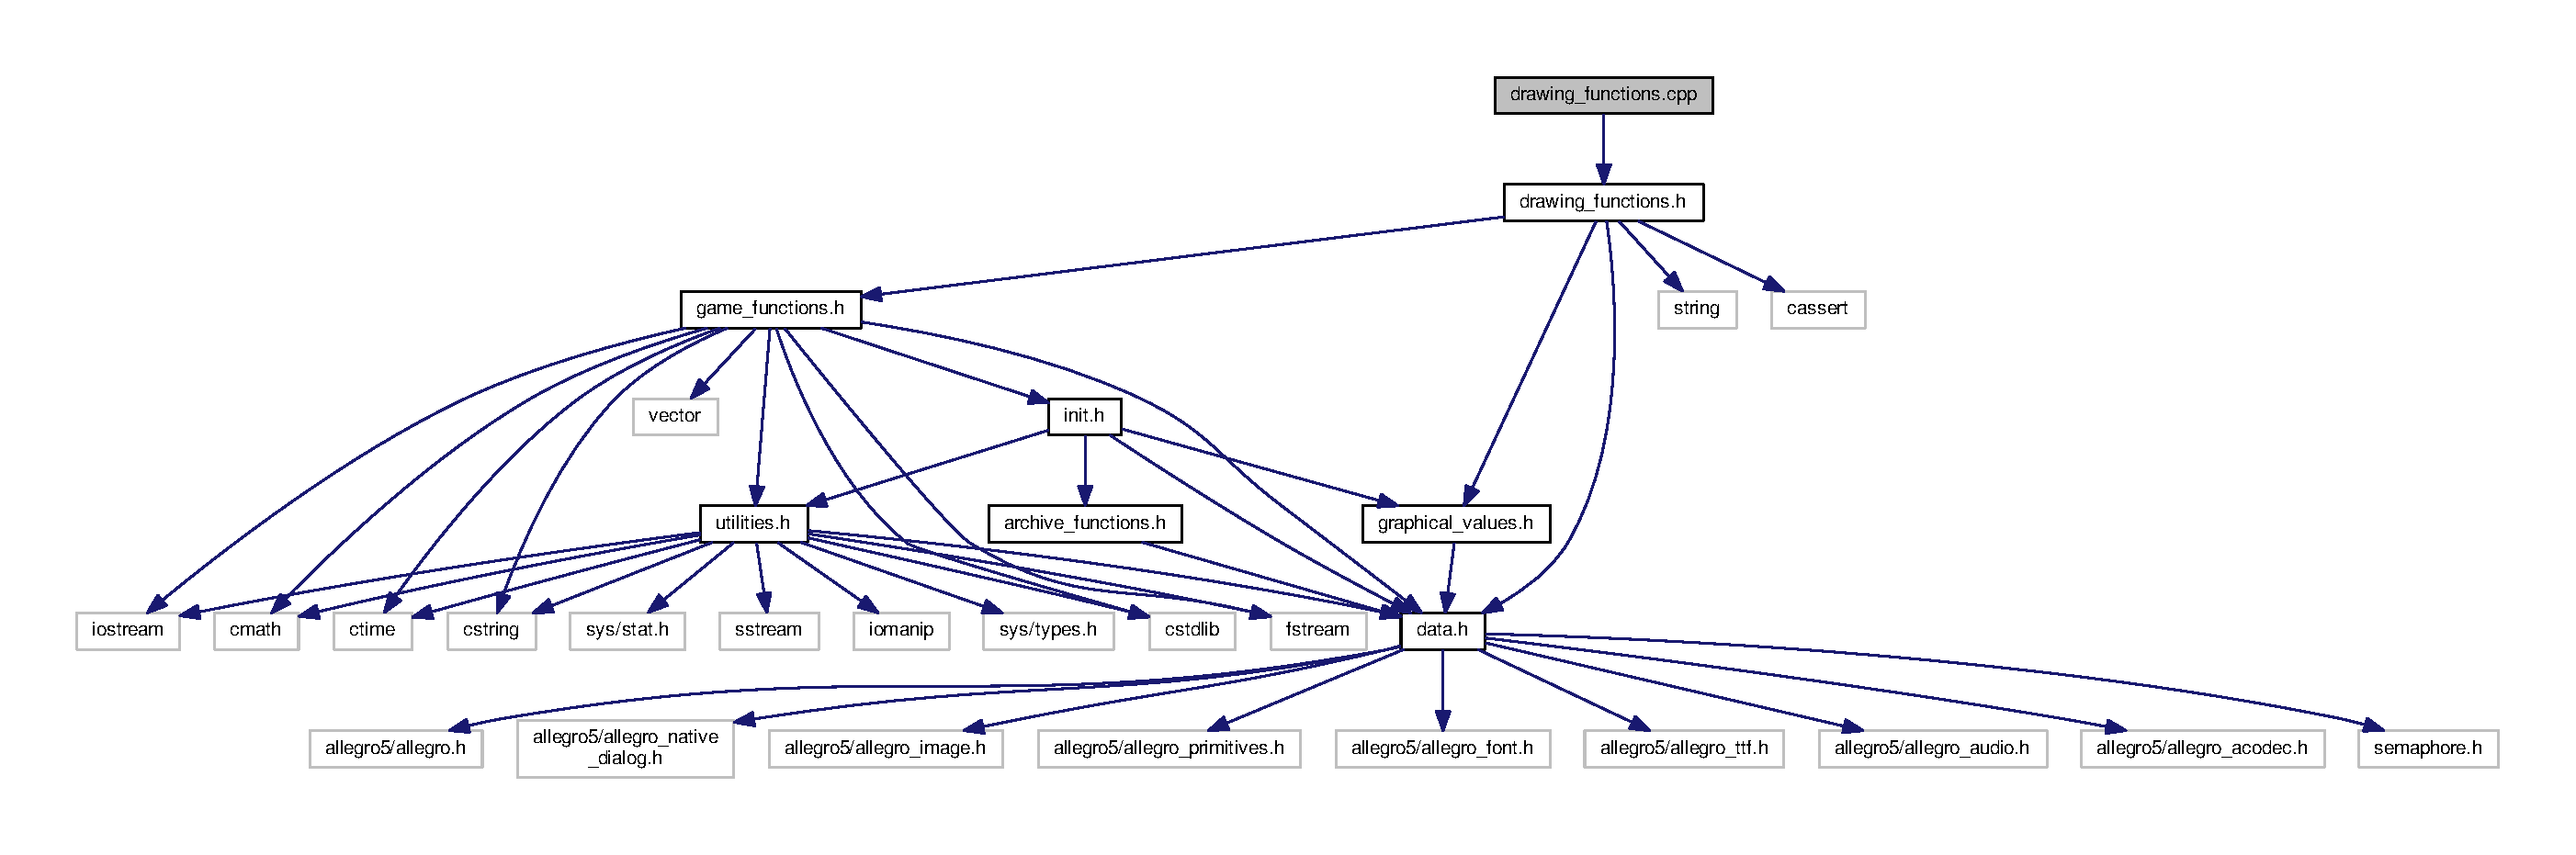
\includegraphics[width=350pt]{df/d63/drawing__functions_8cpp__incl}
\end{center}
\end{figure}
\subsection*{Funzioni}
\begin{DoxyCompactItemize}
\item 
A\+L\+L\+E\+G\+R\+O\+\_\+\+B\+I\+T\+M\+AP $\ast$$\ast$ \hyperlink{drawing__functions_8cpp_a4c5bc668d5d515156097d50ad1ea094c}{generate\+\_\+menu\+\_\+bitmaps} ()
\begin{DoxyCompactList}\small\item\em Funzione che genera l\textquotesingle{}array contenente i puntatori ai bitmap relativi alla schermata del menu principale. \end{DoxyCompactList}\item 
A\+L\+L\+E\+G\+R\+O\+\_\+\+B\+I\+T\+M\+AP $\ast$$\ast$ \hyperlink{drawing__functions_8cpp_acaa107eaf4d6d8e1e1675d3e7c576277}{generate\+\_\+playwa\+\_\+bitmaps} ()
\begin{DoxyCompactList}\small\item\em Funzione che genera l\textquotesingle{}array contenente i puntatori ai bitmap relativi alla schermata di gioco. \end{DoxyCompactList}\item 
A\+L\+L\+E\+G\+R\+O\+\_\+\+B\+I\+T\+M\+AP $\ast$$\ast$ \hyperlink{drawing__functions_8cpp_a63f87e78d7d8340b2a5a02dc56b61718}{generate\+\_\+instr\+\_\+bitmaps} ()
\begin{DoxyCompactList}\small\item\em Funzione che genera l\textquotesingle{}array contenente i puntatori ai bitmap relativi alla schermata di pausa. \end{DoxyCompactList}\item 
A\+L\+L\+E\+G\+R\+O\+\_\+\+F\+O\+NT $\ast$$\ast$ \hyperlink{drawing__functions_8cpp_a73982fb9ed5faaa34dd83cec1c8deb7c}{generate\+\_\+playwa\+\_\+fonts} ()
\begin{DoxyCompactList}\small\item\em Funzione che genera l\textquotesingle{}array contenente i puntatori ai font relativi alla schermata di gioco. \end{DoxyCompactList}\item 
A\+L\+L\+E\+G\+R\+O\+\_\+\+F\+O\+NT $\ast$$\ast$ \hyperlink{drawing__functions_8cpp_a91ed375d606dbda8bdeaefde045bccc0}{generate\+\_\+instr\+\_\+fonts} ()
\begin{DoxyCompactList}\small\item\em Funzione che genera l\textquotesingle{}array contenente i puntatori ai font relativi alla schermata di pausa. \end{DoxyCompactList}\item 
A\+L\+L\+E\+G\+R\+O\+\_\+\+F\+O\+NT $\ast$$\ast$ \hyperlink{drawing__functions_8cpp_ac8a42fd07fd0472609d1334c696ca934}{generate\+\_\+menu\+\_\+fonts} ()
\begin{DoxyCompactList}\small\item\em Funzione che genera l\textquotesingle{}array contenente i puntatori ai font relativi ai menu. \end{DoxyCompactList}\item 
A\+L\+L\+E\+G\+R\+O\+\_\+\+F\+O\+NT $\ast$$\ast$ \hyperlink{drawing__functions_8cpp_ae2818bfb00fa513611854338aeeef6ad}{generate\+\_\+user\+\_\+fonts} ()
\begin{DoxyCompactList}\small\item\em Funzione che genera l\textquotesingle{}array contenente i puntatori ai font relativi alla schermata di gameover. \end{DoxyCompactList}\item 
A\+L\+L\+E\+G\+R\+O\+\_\+\+F\+O\+NT $\ast$$\ast$ \hyperlink{drawing__functions_8cpp_ae4246ed2992a4852e394233e2b41d013}{generate\+\_\+settings\+\_\+fonts} ()
\begin{DoxyCompactList}\small\item\em Funzione che genera l\textquotesingle{}array contenente i puntatori ai font relativi alla schermata delle impostazioni. \end{DoxyCompactList}\item 
void \hyperlink{drawing__functions_8cpp_a30bcdca4f2bc932add7319374a3bb617}{destroy\+\_\+arr\+\_\+bitmaps} (A\+L\+L\+E\+G\+R\+O\+\_\+\+B\+I\+T\+M\+AP $\ast$$\ast$arr, const int num)
\begin{DoxyCompactList}\small\item\em Funzione che dealloca un array di bitmap, oltre che tutti i bitmap in esso contenuti. \end{DoxyCompactList}\item 
void \hyperlink{drawing__functions_8cpp_a3c93cba6ceb2ca7188621e0112220c8c}{destroy\+\_\+arr\+\_\+fonts} (A\+L\+L\+E\+G\+R\+O\+\_\+\+F\+O\+NT $\ast$$\ast$arr, const int num)
\begin{DoxyCompactList}\small\item\em Funzione che dealloca un array di font, oltre che tutti i font in esso contenuti. \end{DoxyCompactList}\item 
void \hyperlink{drawing__functions_8cpp_ae6b0d0c9d9a687608caf2b5f240758cf}{draw\+\_\+background} (A\+L\+L\+E\+G\+R\+O\+\_\+\+B\+I\+T\+M\+AP $\ast$bmp\+\_\+bg, float \&offset\+\_\+bg, const bool playing)
\begin{DoxyCompactList}\small\item\em Funzione che stampa lo sfondo della schermata. \end{DoxyCompactList}\item 
void \hyperlink{drawing__functions_8cpp_a1fc8105c4e2716aff11b7f1835be51b9}{draw\+\_\+head} (char $\ast$head\+\_\+str, A\+L\+L\+E\+G\+R\+O\+\_\+\+F\+O\+NT $\ast$font)
\begin{DoxyCompactList}\small\item\em Funzione che stampa il titolo della schermata. \end{DoxyCompactList}\item 
void \hyperlink{drawing__functions_8cpp_a5492eb7b0241c0d2cc97cda425addebd}{draw\+\_\+back} (A\+L\+L\+E\+G\+R\+O\+\_\+\+F\+O\+NT $\ast$font, const bool pause)
\begin{DoxyCompactList}\small\item\em Funzione che stampa la stringa di ritorno al gioco, o al menu principale (in base alla variabile \char`\"{}pause\char`\"{}). \end{DoxyCompactList}\item 
void \hyperlink{drawing__functions_8cpp_a497ccfc6d0c0bf91883fa091a8fc9310}{draw\+\_\+intro\+\_\+init} (A\+L\+L\+E\+G\+R\+O\+\_\+\+B\+I\+T\+M\+AP $\ast$$\ast$arr\+\_\+bitmaps, float \&bg\+\_\+offset)
\begin{DoxyCompactList}\small\item\em Funzione che gestisce l\textquotesingle{}inizializzazione dell\textquotesingle{}animazione di introduzione. \end{DoxyCompactList}\item 
void \hyperlink{drawing__functions_8cpp_adc09c13b7ec3fb805900982610c49cf9}{draw\+\_\+intro\+\_\+title\+\_\+slide} (A\+L\+L\+E\+G\+R\+O\+\_\+\+B\+I\+T\+M\+AP $\ast$$\ast$arr\+\_\+bitmaps, float \&bg\+\_\+offset)
\begin{DoxyCompactList}\small\item\em Funzione che gestisce lo slide del titolo nell\textquotesingle{}animazione di introduzione. \end{DoxyCompactList}\item 
void \hyperlink{drawing__functions_8cpp_a51a2880bf7e514344ee1ac5e562f9479}{draw\+\_\+intro\+\_\+menu\+\_\+fadein} (A\+L\+L\+E\+G\+R\+O\+\_\+\+B\+I\+T\+M\+AP $\ast$$\ast$arr\+\_\+bitmaps, A\+L\+L\+E\+G\+R\+O\+\_\+\+F\+O\+NT $\ast$$\ast$arr\+\_\+fonts, float \&bg\+\_\+offset)
\begin{DoxyCompactList}\small\item\em Funzione che gestisce il fadein del menu nell\textquotesingle{}animazione di introduzione. \end{DoxyCompactList}\item 
void \hyperlink{drawing__functions_8cpp_a9affe6a634fbf578ab2158cb6ae5ae7f}{draw\+\_\+menu\+\_\+title} (A\+L\+L\+E\+G\+R\+O\+\_\+\+B\+I\+T\+M\+AP $\ast$bmp\+\_\+title)
\begin{DoxyCompactList}\small\item\em Funzione che stampa il bitmap relativo al titolo presente nel menu principale. \end{DoxyCompactList}\item 
void \hyperlink{drawing__functions_8cpp_a9ce95bf12fc8789ae26027859ee5f47d}{draw\+\_\+menu\+\_\+option} (const int \&index, A\+L\+L\+E\+G\+R\+O\+\_\+\+B\+I\+T\+M\+AP $\ast$bmp\+\_\+option, A\+L\+L\+E\+G\+R\+O\+\_\+\+F\+O\+NT $\ast$font, char $\ast$str\+\_\+scelta, const bool settings)
\begin{DoxyCompactList}\small\item\em Funzione che stampa l\textquotesingle{}opzione indicata (menu). \end{DoxyCompactList}\item 
void \hyperlink{drawing__functions_8cpp_aa6d5deb3a6b2e9f1a2db69ff00badcbb}{draw\+\_\+menu\+\_\+copyright} (A\+L\+L\+E\+G\+R\+O\+\_\+\+F\+O\+NT $\ast$font)
\begin{DoxyCompactList}\small\item\em Funzione che stampa la stringa di copyright (menu). \end{DoxyCompactList}\item 
void \hyperlink{drawing__functions_8cpp_afcf3a6ebbfad9889b2b58b85f82814c7}{draw\+\_\+playwa\+\_\+score\+\_\+hint} (const \hyperlink{structmatch__vars__t}{match\+\_\+vars\+\_\+t} \&match\+\_\+vars, A\+L\+L\+E\+G\+R\+O\+\_\+\+F\+O\+NT $\ast$font\+\_\+score, A\+L\+L\+E\+G\+R\+O\+\_\+\+F\+O\+NT $\ast$font\+\_\+hints, const bool visible\+\_\+hints)
\begin{DoxyCompactList}\small\item\em Funzione che stampa il punteggio e i suggerimenti (schermata di gioco). \end{DoxyCompactList}\item 
void \hyperlink{drawing__functions_8cpp_aa12cd18d497401592c40fd5f803ed384}{draw\+\_\+playwa\+\_\+shooter} (const \hyperlink{structmatch__vars__t}{match\+\_\+vars\+\_\+t} \&match\+\_\+vars, const \hyperlink{structbullet__t}{bullet\+\_\+t} $\ast$arr\+\_\+bullet, const \hyperlink{structshooter__t}{shooter\+\_\+t} \&shooter, A\+L\+L\+E\+G\+R\+O\+\_\+\+B\+I\+T\+M\+AP $\ast$$\ast$arr\+\_\+bitmaps)
\begin{DoxyCompactList}\small\item\em Funzione che stampa lo shooter, la sua area (bianca normalmente, rossa in caso di pericolo o azzurra nel caso in cui il bonus \char`\"{}shield\char`\"{} venga attivato). \end{DoxyCompactList}\item 
void \hyperlink{drawing__functions_8cpp_a61d883b04452e38f3c290857d66941d7}{draw\+\_\+playwa\+\_\+asteroids\+\_\+bullets} (const \hyperlink{structmatch__vars__t}{match\+\_\+vars\+\_\+t} \&match\+\_\+vars, const \hyperlink{structbullet__t}{bullet\+\_\+t} $\ast$arr\+\_\+bullet, A\+L\+L\+E\+G\+R\+O\+\_\+\+B\+I\+T\+M\+AP $\ast$$\ast$arr\+\_\+bitmaps, A\+L\+L\+E\+G\+R\+O\+\_\+\+F\+O\+NT $\ast$font)
\begin{DoxyCompactList}\small\item\em Funzione che stampa lo gli asteroidi ed i proiettili presenti in gioco. \end{DoxyCompactList}\item 
void \hyperlink{drawing__functions_8cpp_acac0972652d8d16bcebdc571bd69d7cc}{draw\+\_\+playwa\+\_\+bonus\+\_\+music} (const \hyperlink{structmatch__vars__t}{match\+\_\+vars\+\_\+t} \&match\+\_\+vars, A\+L\+L\+E\+G\+R\+O\+\_\+\+B\+I\+T\+M\+AP $\ast$$\ast$arr\+\_\+bitmaps, A\+L\+L\+E\+G\+R\+O\+\_\+\+F\+O\+NT $\ast$font\+\_\+score, A\+L\+L\+E\+G\+R\+O\+\_\+\+F\+O\+NT $\ast$font\+\_\+bonus, A\+L\+L\+E\+G\+R\+O\+\_\+\+F\+O\+NT $\ast$font\+\_\+bonus\+\_\+hint, \hyperlink{structsettings__t}{settings\+\_\+t} settings)
\begin{DoxyCompactList}\small\item\em Funzione che stampa i bonus della partita (e le icone relative al suono). \end{DoxyCompactList}\item 
void \hyperlink{drawing__functions_8cpp_a3bf614e725835505499415b255bff0e7}{draw\+\_\+stats\+\_\+blocks} (A\+L\+L\+E\+G\+R\+O\+\_\+\+F\+O\+NT $\ast$font)
\begin{DoxyCompactList}\small\item\em Funzione che disegna i blocchi di sfondo relativi ai risultati di fine partita. \end{DoxyCompactList}\item 
void \hyperlink{drawing__functions_8cpp_a7f0ecbefa0f7f7cb274e8d5b56c3aa74}{draw\+\_\+stat} (const int \&idx\+\_\+stat, int stat\+\_\+value, A\+L\+L\+E\+G\+R\+O\+\_\+\+F\+O\+NT $\ast$font)
\begin{DoxyCompactList}\small\item\em Funzione che disegna un singolo risultato. \end{DoxyCompactList}\item 
void \hyperlink{drawing__functions_8cpp_a05c0e4929a232f4cdcfbf43b05c79b39}{draw\+\_\+gameover\+\_\+animation} (const int \&score\+\_\+goal, const int \&dast\+\_\+goal, A\+L\+L\+E\+G\+R\+O\+\_\+\+B\+I\+T\+M\+AP $\ast$bg\+\_\+bmp, float \&bg\+\_\+offset, A\+L\+L\+E\+G\+R\+O\+\_\+\+F\+O\+NT $\ast$$\ast$arr\+\_\+fonts)
\begin{DoxyCompactList}\small\item\em Funzione che gestisce l\textquotesingle{}animazione di fine partita. \end{DoxyCompactList}\item 
void \hyperlink{drawing__functions_8cpp_ad713eae96f263309068c67fe145b9748}{draw\+\_\+playagain\+\_\+button} (A\+L\+L\+E\+G\+R\+O\+\_\+\+F\+O\+NT $\ast$font)
\begin{DoxyCompactList}\small\item\em Funzione che disegna il bottone \char`\"{}play again\char`\"{} nella schermata di Game Over. \end{DoxyCompactList}\item 
void \hyperlink{drawing__functions_8cpp_ada8f618047616bdecf221bf0548fd2e5}{draw\+\_\+results} (A\+L\+L\+E\+G\+R\+O\+\_\+\+F\+O\+NT $\ast$font, \hyperlink{structresult__t}{result\+\_\+t} res)
\begin{DoxyCompactList}\small\item\em Funzione che disegna i risultati estratti dagli archivi corrispondenti alla password inserita dell\textquotesingle{}utente. \end{DoxyCompactList}\item 
void \hyperlink{drawing__functions_8cpp_acf0b8be217a189ac8895e0a879931602}{draw\+\_\+username\+\_\+block} (const bool enter\+\_\+active, A\+L\+L\+E\+G\+R\+O\+\_\+\+F\+O\+NT $\ast$font)
\begin{DoxyCompactList}\small\item\em Funzione che disegna il blocco di inserimento dello username. \end{DoxyCompactList}\item 
void \hyperlink{drawing__functions_8cpp_a6d58b45f3a62d5d1fd44a26e3e206c72}{draw\+\_\+username} (char $\ast$username, const int \&cur\+\_\+pos, A\+L\+L\+E\+G\+R\+O\+\_\+\+F\+O\+NT $\ast$font, const bool bar\+\_\+visible)
\begin{DoxyCompactList}\small\item\em Funzione che disegna lo username. \end{DoxyCompactList}\item 
void \hyperlink{drawing__functions_8cpp_a7b076accc9ae9e5e8e5e172d9bc50e8f}{draw\+\_\+instructions} (A\+L\+L\+E\+G\+R\+O\+\_\+\+F\+O\+NT $\ast$$\ast$arr\+\_\+fonts, A\+L\+L\+E\+G\+R\+O\+\_\+\+B\+I\+T\+M\+AP $\ast$$\ast$arr\+\_\+bitmaps)
\begin{DoxyCompactList}\small\item\em Funzine che disegna le istruzioni durante la pausa. \end{DoxyCompactList}\end{DoxyCompactItemize}


\subsection{Documentazione delle funzioni}
\mbox{\Hypertarget{drawing__functions_8cpp_a30bcdca4f2bc932add7319374a3bb617}\label{drawing__functions_8cpp_a30bcdca4f2bc932add7319374a3bb617}} 
\index{drawing\+\_\+functions.\+cpp@{drawing\+\_\+functions.\+cpp}!destroy\+\_\+arr\+\_\+bitmaps@{destroy\+\_\+arr\+\_\+bitmaps}}
\index{destroy\+\_\+arr\+\_\+bitmaps@{destroy\+\_\+arr\+\_\+bitmaps}!drawing\+\_\+functions.\+cpp@{drawing\+\_\+functions.\+cpp}}
\subsubsection{\texorpdfstring{destroy\+\_\+arr\+\_\+bitmaps()}{destroy\_arr\_bitmaps()}}
{\footnotesize\ttfamily void destroy\+\_\+arr\+\_\+bitmaps (\begin{DoxyParamCaption}\item[{A\+L\+L\+E\+G\+R\+O\+\_\+\+B\+I\+T\+M\+AP $\ast$$\ast$}]{arr,  }\item[{const int}]{num }\end{DoxyParamCaption})}



Funzione che dealloca un array di bitmap, oltre che tutti i bitmap in esso contenuti. 

~\newline
Parametri\+: ~\newline
1) arr -\/ Array di bitmap; ~\newline
2) num -\/ Dimensione dell\textquotesingle{}array di bitmap. \mbox{\Hypertarget{drawing__functions_8cpp_a3c93cba6ceb2ca7188621e0112220c8c}\label{drawing__functions_8cpp_a3c93cba6ceb2ca7188621e0112220c8c}} 
\index{drawing\+\_\+functions.\+cpp@{drawing\+\_\+functions.\+cpp}!destroy\+\_\+arr\+\_\+fonts@{destroy\+\_\+arr\+\_\+fonts}}
\index{destroy\+\_\+arr\+\_\+fonts@{destroy\+\_\+arr\+\_\+fonts}!drawing\+\_\+functions.\+cpp@{drawing\+\_\+functions.\+cpp}}
\subsubsection{\texorpdfstring{destroy\+\_\+arr\+\_\+fonts()}{destroy\_arr\_fonts()}}
{\footnotesize\ttfamily void destroy\+\_\+arr\+\_\+fonts (\begin{DoxyParamCaption}\item[{A\+L\+L\+E\+G\+R\+O\+\_\+\+F\+O\+NT $\ast$$\ast$}]{arr,  }\item[{const int}]{num }\end{DoxyParamCaption})}



Funzione che dealloca un array di font, oltre che tutti i font in esso contenuti. 

~\newline
Parametri\+: ~\newline
1) arr -\/ Array di font; ~\newline
2) num -\/ Dimensione dell\textquotesingle{}array di font. \mbox{\Hypertarget{drawing__functions_8cpp_a5492eb7b0241c0d2cc97cda425addebd}\label{drawing__functions_8cpp_a5492eb7b0241c0d2cc97cda425addebd}} 
\index{drawing\+\_\+functions.\+cpp@{drawing\+\_\+functions.\+cpp}!draw\+\_\+back@{draw\+\_\+back}}
\index{draw\+\_\+back@{draw\+\_\+back}!drawing\+\_\+functions.\+cpp@{drawing\+\_\+functions.\+cpp}}
\subsubsection{\texorpdfstring{draw\+\_\+back()}{draw\_back()}}
{\footnotesize\ttfamily void draw\+\_\+back (\begin{DoxyParamCaption}\item[{A\+L\+L\+E\+G\+R\+O\+\_\+\+F\+O\+NT $\ast$}]{font,  }\item[{const bool}]{pause }\end{DoxyParamCaption})}



Funzione che stampa la stringa di ritorno al gioco, o al menu principale (in base alla variabile \char`\"{}pause\char`\"{}). 

~\newline
Parametri\+: ~\newline
1) font -\/ Font relativo alla stringa di ritorno; ~\newline
2) pause -\/ In base al valore assunto da questa variabile viene stampata la stringa adatta. \mbox{\Hypertarget{drawing__functions_8cpp_ae6b0d0c9d9a687608caf2b5f240758cf}\label{drawing__functions_8cpp_ae6b0d0c9d9a687608caf2b5f240758cf}} 
\index{drawing\+\_\+functions.\+cpp@{drawing\+\_\+functions.\+cpp}!draw\+\_\+background@{draw\+\_\+background}}
\index{draw\+\_\+background@{draw\+\_\+background}!drawing\+\_\+functions.\+cpp@{drawing\+\_\+functions.\+cpp}}
\subsubsection{\texorpdfstring{draw\+\_\+background()}{draw\_background()}}
{\footnotesize\ttfamily void draw\+\_\+background (\begin{DoxyParamCaption}\item[{A\+L\+L\+E\+G\+R\+O\+\_\+\+B\+I\+T\+M\+AP $\ast$}]{bmp\+\_\+bg,  }\item[{float \&}]{offset\+\_\+bg,  }\item[{const bool}]{playing }\end{DoxyParamCaption})}



Funzione che stampa lo sfondo della schermata. 

~\newline
Parametri\+: ~\newline
1) bmp\+\_\+bg -\/ Bitmap relativo allo sfondo; ~\newline
2) offset\+\_\+bg -\/ Scostamento in pixel dello sfondo dal lato sinistro della schermata (per rotazione sfondo); ~\newline
3) playing -\/ Flag sul quale si basa la velocità di rotazione (durante il gioco risulta essere più lenta). \mbox{\Hypertarget{drawing__functions_8cpp_a05c0e4929a232f4cdcfbf43b05c79b39}\label{drawing__functions_8cpp_a05c0e4929a232f4cdcfbf43b05c79b39}} 
\index{drawing\+\_\+functions.\+cpp@{drawing\+\_\+functions.\+cpp}!draw\+\_\+gameover\+\_\+animation@{draw\+\_\+gameover\+\_\+animation}}
\index{draw\+\_\+gameover\+\_\+animation@{draw\+\_\+gameover\+\_\+animation}!drawing\+\_\+functions.\+cpp@{drawing\+\_\+functions.\+cpp}}
\subsubsection{\texorpdfstring{draw\+\_\+gameover\+\_\+animation()}{draw\_gameover\_animation()}}
{\footnotesize\ttfamily void draw\+\_\+gameover\+\_\+animation (\begin{DoxyParamCaption}\item[{const int \&}]{score\+\_\+goal,  }\item[{const int \&}]{dast\+\_\+goal,  }\item[{A\+L\+L\+E\+G\+R\+O\+\_\+\+B\+I\+T\+M\+AP $\ast$}]{bg\+\_\+bmp,  }\item[{float \&}]{bg\+\_\+offset,  }\item[{A\+L\+L\+E\+G\+R\+O\+\_\+\+F\+O\+NT $\ast$$\ast$}]{arr\+\_\+fonts }\end{DoxyParamCaption})}



Funzione che gestisce l\textquotesingle{}animazione di fine partita. 

~\newline
Parametri\+: ~\newline
1) score\+\_\+goal -\/ Score effettiva del giocatore; ~\newline
2) dast\+\_\+goal -\/ Asteroidi effettivamente distrutti; ~\newline
4) bg\+\_\+bmp -\/ Bitmap di sfondo; ~\newline
5) bg\+\_\+offset -\/ Scostamento laterale dello sfondo; ~\newline
6) arr\+\_\+fonts -\/ Array dei font necessari. \mbox{\Hypertarget{drawing__functions_8cpp_a1fc8105c4e2716aff11b7f1835be51b9}\label{drawing__functions_8cpp_a1fc8105c4e2716aff11b7f1835be51b9}} 
\index{drawing\+\_\+functions.\+cpp@{drawing\+\_\+functions.\+cpp}!draw\+\_\+head@{draw\+\_\+head}}
\index{draw\+\_\+head@{draw\+\_\+head}!drawing\+\_\+functions.\+cpp@{drawing\+\_\+functions.\+cpp}}
\subsubsection{\texorpdfstring{draw\+\_\+head()}{draw\_head()}}
{\footnotesize\ttfamily void draw\+\_\+head (\begin{DoxyParamCaption}\item[{char $\ast$}]{head\+\_\+str,  }\item[{A\+L\+L\+E\+G\+R\+O\+\_\+\+F\+O\+NT $\ast$}]{font }\end{DoxyParamCaption})}



Funzione che stampa il titolo della schermata. 

~\newline
Parametri\+: ~\newline
1) head\+\_\+str -\/ Stringa relativa al titolo; ~\newline
2) font -\/ Font relativo al titolo. \mbox{\Hypertarget{drawing__functions_8cpp_a7b076accc9ae9e5e8e5e172d9bc50e8f}\label{drawing__functions_8cpp_a7b076accc9ae9e5e8e5e172d9bc50e8f}} 
\index{drawing\+\_\+functions.\+cpp@{drawing\+\_\+functions.\+cpp}!draw\+\_\+instructions@{draw\+\_\+instructions}}
\index{draw\+\_\+instructions@{draw\+\_\+instructions}!drawing\+\_\+functions.\+cpp@{drawing\+\_\+functions.\+cpp}}
\subsubsection{\texorpdfstring{draw\+\_\+instructions()}{draw\_instructions()}}
{\footnotesize\ttfamily void draw\+\_\+instructions (\begin{DoxyParamCaption}\item[{A\+L\+L\+E\+G\+R\+O\+\_\+\+F\+O\+NT $\ast$$\ast$}]{arr\+\_\+fonts,  }\item[{A\+L\+L\+E\+G\+R\+O\+\_\+\+B\+I\+T\+M\+AP $\ast$$\ast$}]{arr\+\_\+bitmaps }\end{DoxyParamCaption})}



Funzine che disegna le istruzioni durante la pausa. 

~\newline
Parametri\+: ~\newline
1) arr\+\_\+fonts -\/ Array contenente i font utilizzati; ~\newline
2) arr\+\_\+bitmaps -\/ Array contenente i bitmap utilizzati. \mbox{\Hypertarget{drawing__functions_8cpp_a497ccfc6d0c0bf91883fa091a8fc9310}\label{drawing__functions_8cpp_a497ccfc6d0c0bf91883fa091a8fc9310}} 
\index{drawing\+\_\+functions.\+cpp@{drawing\+\_\+functions.\+cpp}!draw\+\_\+intro\+\_\+init@{draw\+\_\+intro\+\_\+init}}
\index{draw\+\_\+intro\+\_\+init@{draw\+\_\+intro\+\_\+init}!drawing\+\_\+functions.\+cpp@{drawing\+\_\+functions.\+cpp}}
\subsubsection{\texorpdfstring{draw\+\_\+intro\+\_\+init()}{draw\_intro\_init()}}
{\footnotesize\ttfamily void draw\+\_\+intro\+\_\+init (\begin{DoxyParamCaption}\item[{A\+L\+L\+E\+G\+R\+O\+\_\+\+B\+I\+T\+M\+AP $\ast$$\ast$}]{arr\+\_\+bitmaps,  }\item[{float \&}]{bg\+\_\+offset }\end{DoxyParamCaption})}



Funzione che gestisce l\textquotesingle{}inizializzazione dell\textquotesingle{}animazione di introduzione. 

~\newline
Parametri\+: ~\newline
1) arr\+\_\+bitmaps -\/ Array di bitmap; ~\newline
2) bg\+\_\+offset -\/ Offset iniziale dello sfondo. \mbox{\Hypertarget{drawing__functions_8cpp_a51a2880bf7e514344ee1ac5e562f9479}\label{drawing__functions_8cpp_a51a2880bf7e514344ee1ac5e562f9479}} 
\index{drawing\+\_\+functions.\+cpp@{drawing\+\_\+functions.\+cpp}!draw\+\_\+intro\+\_\+menu\+\_\+fadein@{draw\+\_\+intro\+\_\+menu\+\_\+fadein}}
\index{draw\+\_\+intro\+\_\+menu\+\_\+fadein@{draw\+\_\+intro\+\_\+menu\+\_\+fadein}!drawing\+\_\+functions.\+cpp@{drawing\+\_\+functions.\+cpp}}
\subsubsection{\texorpdfstring{draw\+\_\+intro\+\_\+menu\+\_\+fadein()}{draw\_intro\_menu\_fadein()}}
{\footnotesize\ttfamily void draw\+\_\+intro\+\_\+menu\+\_\+fadein (\begin{DoxyParamCaption}\item[{A\+L\+L\+E\+G\+R\+O\+\_\+\+B\+I\+T\+M\+AP $\ast$$\ast$}]{arr\+\_\+bitmaps,  }\item[{A\+L\+L\+E\+G\+R\+O\+\_\+\+F\+O\+NT $\ast$$\ast$}]{arr\+\_\+fonts,  }\item[{float \&}]{bg\+\_\+offset }\end{DoxyParamCaption})}



Funzione che gestisce il fadein del menu nell\textquotesingle{}animazione di introduzione. 

~\newline
Parametri\+: ~\newline
1) arr\+\_\+bitmaps -\/ Array di bitmap; ~\newline
2) arr\+\_\+fonts -\/ Array di font; ~\newline
3) bg\+\_\+offset -\/ Offset iniziale dello sfondo. \mbox{\Hypertarget{drawing__functions_8cpp_adc09c13b7ec3fb805900982610c49cf9}\label{drawing__functions_8cpp_adc09c13b7ec3fb805900982610c49cf9}} 
\index{drawing\+\_\+functions.\+cpp@{drawing\+\_\+functions.\+cpp}!draw\+\_\+intro\+\_\+title\+\_\+slide@{draw\+\_\+intro\+\_\+title\+\_\+slide}}
\index{draw\+\_\+intro\+\_\+title\+\_\+slide@{draw\+\_\+intro\+\_\+title\+\_\+slide}!drawing\+\_\+functions.\+cpp@{drawing\+\_\+functions.\+cpp}}
\subsubsection{\texorpdfstring{draw\+\_\+intro\+\_\+title\+\_\+slide()}{draw\_intro\_title\_slide()}}
{\footnotesize\ttfamily void draw\+\_\+intro\+\_\+title\+\_\+slide (\begin{DoxyParamCaption}\item[{A\+L\+L\+E\+G\+R\+O\+\_\+\+B\+I\+T\+M\+AP $\ast$$\ast$}]{arr\+\_\+bitmaps,  }\item[{float \&}]{bg\+\_\+offset }\end{DoxyParamCaption})}



Funzione che gestisce lo slide del titolo nell\textquotesingle{}animazione di introduzione. 

~\newline
Parametri\+: ~\newline
1) arr\+\_\+bitmaps -\/ Array di bitmap; ~\newline
2) bg\+\_\+offset -\/ Offset iniziale dello sfondo. \mbox{\Hypertarget{drawing__functions_8cpp_aa6d5deb3a6b2e9f1a2db69ff00badcbb}\label{drawing__functions_8cpp_aa6d5deb3a6b2e9f1a2db69ff00badcbb}} 
\index{drawing\+\_\+functions.\+cpp@{drawing\+\_\+functions.\+cpp}!draw\+\_\+menu\+\_\+copyright@{draw\+\_\+menu\+\_\+copyright}}
\index{draw\+\_\+menu\+\_\+copyright@{draw\+\_\+menu\+\_\+copyright}!drawing\+\_\+functions.\+cpp@{drawing\+\_\+functions.\+cpp}}
\subsubsection{\texorpdfstring{draw\+\_\+menu\+\_\+copyright()}{draw\_menu\_copyright()}}
{\footnotesize\ttfamily void draw\+\_\+menu\+\_\+copyright (\begin{DoxyParamCaption}\item[{A\+L\+L\+E\+G\+R\+O\+\_\+\+F\+O\+NT $\ast$}]{font }\end{DoxyParamCaption})}



Funzione che stampa la stringa di copyright (menu). 

~\newline
Parametri\+: ~\newline
1) font -\/ Font relativo alla stringa di copyright. \mbox{\Hypertarget{drawing__functions_8cpp_a9ce95bf12fc8789ae26027859ee5f47d}\label{drawing__functions_8cpp_a9ce95bf12fc8789ae26027859ee5f47d}} 
\index{drawing\+\_\+functions.\+cpp@{drawing\+\_\+functions.\+cpp}!draw\+\_\+menu\+\_\+option@{draw\+\_\+menu\+\_\+option}}
\index{draw\+\_\+menu\+\_\+option@{draw\+\_\+menu\+\_\+option}!drawing\+\_\+functions.\+cpp@{drawing\+\_\+functions.\+cpp}}
\subsubsection{\texorpdfstring{draw\+\_\+menu\+\_\+option()}{draw\_menu\_option()}}
{\footnotesize\ttfamily void draw\+\_\+menu\+\_\+option (\begin{DoxyParamCaption}\item[{const int \&}]{index,  }\item[{A\+L\+L\+E\+G\+R\+O\+\_\+\+B\+I\+T\+M\+AP $\ast$}]{bmp\+\_\+option,  }\item[{A\+L\+L\+E\+G\+R\+O\+\_\+\+F\+O\+NT $\ast$}]{font,  }\item[{char $\ast$}]{str\+\_\+scelta,  }\item[{const bool}]{settings }\end{DoxyParamCaption})}



Funzione che stampa l\textquotesingle{}opzione indicata (menu). 

~\newline
Parametri\+: ~\newline
1) index -\/ Indice dell\textquotesingle{}opzione; ~\newline
2) bmp\+\_\+option -\/ Bitmap relativo all\textquotesingle{}opzione indicata; ~\newline
3) font -\/ Font relativo all\textquotesingle{}opzione indicata; ~\newline
4) str\+\_\+scelta -\/ Stringa relativa all\textquotesingle{}opzione indicata; ~\newline
5) settings -\/ Se vero, stampa le opzioni leggermente più in alto rispetto al menu principale. \mbox{\Hypertarget{drawing__functions_8cpp_a9affe6a634fbf578ab2158cb6ae5ae7f}\label{drawing__functions_8cpp_a9affe6a634fbf578ab2158cb6ae5ae7f}} 
\index{drawing\+\_\+functions.\+cpp@{drawing\+\_\+functions.\+cpp}!draw\+\_\+menu\+\_\+title@{draw\+\_\+menu\+\_\+title}}
\index{draw\+\_\+menu\+\_\+title@{draw\+\_\+menu\+\_\+title}!drawing\+\_\+functions.\+cpp@{drawing\+\_\+functions.\+cpp}}
\subsubsection{\texorpdfstring{draw\+\_\+menu\+\_\+title()}{draw\_menu\_title()}}
{\footnotesize\ttfamily void draw\+\_\+menu\+\_\+title (\begin{DoxyParamCaption}\item[{A\+L\+L\+E\+G\+R\+O\+\_\+\+B\+I\+T\+M\+AP $\ast$}]{bmp\+\_\+title }\end{DoxyParamCaption})}



Funzione che stampa il bitmap relativo al titolo presente nel menu principale. 

~\newline
Parametri\+: ~\newline
1) bmp\+\_\+title -\/ Bitmap relativo al titolo. \mbox{\Hypertarget{drawing__functions_8cpp_ad713eae96f263309068c67fe145b9748}\label{drawing__functions_8cpp_ad713eae96f263309068c67fe145b9748}} 
\index{drawing\+\_\+functions.\+cpp@{drawing\+\_\+functions.\+cpp}!draw\+\_\+playagain\+\_\+button@{draw\+\_\+playagain\+\_\+button}}
\index{draw\+\_\+playagain\+\_\+button@{draw\+\_\+playagain\+\_\+button}!drawing\+\_\+functions.\+cpp@{drawing\+\_\+functions.\+cpp}}
\subsubsection{\texorpdfstring{draw\+\_\+playagain\+\_\+button()}{draw\_playagain\_button()}}
{\footnotesize\ttfamily void draw\+\_\+playagain\+\_\+button (\begin{DoxyParamCaption}\item[{A\+L\+L\+E\+G\+R\+O\+\_\+\+F\+O\+NT $\ast$}]{font }\end{DoxyParamCaption})}



Funzione che disegna il bottone \char`\"{}play again\char`\"{} nella schermata di Game Over. 

~\newline
Parametri\+: ~\newline
1) arr\+\_\+fonts -\/ Array dei font necessari;~\newline
\mbox{\Hypertarget{drawing__functions_8cpp_a61d883b04452e38f3c290857d66941d7}\label{drawing__functions_8cpp_a61d883b04452e38f3c290857d66941d7}} 
\index{drawing\+\_\+functions.\+cpp@{drawing\+\_\+functions.\+cpp}!draw\+\_\+playwa\+\_\+asteroids\+\_\+bullets@{draw\+\_\+playwa\+\_\+asteroids\+\_\+bullets}}
\index{draw\+\_\+playwa\+\_\+asteroids\+\_\+bullets@{draw\+\_\+playwa\+\_\+asteroids\+\_\+bullets}!drawing\+\_\+functions.\+cpp@{drawing\+\_\+functions.\+cpp}}
\subsubsection{\texorpdfstring{draw\+\_\+playwa\+\_\+asteroids\+\_\+bullets()}{draw\_playwa\_asteroids\_bullets()}}
{\footnotesize\ttfamily void draw\+\_\+playwa\+\_\+asteroids\+\_\+bullets (\begin{DoxyParamCaption}\item[{const \hyperlink{structmatch__vars__t}{match\+\_\+vars\+\_\+t} \&}]{match\+\_\+vars,  }\item[{const \hyperlink{structbullet__t}{bullet\+\_\+t} $\ast$}]{arr\+\_\+bullet,  }\item[{A\+L\+L\+E\+G\+R\+O\+\_\+\+B\+I\+T\+M\+AP $\ast$$\ast$}]{arr\+\_\+bitmaps,  }\item[{A\+L\+L\+E\+G\+R\+O\+\_\+\+F\+O\+NT $\ast$}]{font }\end{DoxyParamCaption})}



Funzione che stampa lo gli asteroidi ed i proiettili presenti in gioco. 

~\newline
Parametri\+: ~\newline
1) match\+\_\+vars -\/ Struct contenente le variabili di gioco; ~\newline
2) arr\+\_\+bullet -\/ Array contenente i proiettili in gioco; ~\newline
3) arr\+\_\+bitmaps -\/ Array contenente i bitmap di gioco; ~\newline
4) font -\/ Font relativo agli asteroidi. \mbox{\Hypertarget{drawing__functions_8cpp_acac0972652d8d16bcebdc571bd69d7cc}\label{drawing__functions_8cpp_acac0972652d8d16bcebdc571bd69d7cc}} 
\index{drawing\+\_\+functions.\+cpp@{drawing\+\_\+functions.\+cpp}!draw\+\_\+playwa\+\_\+bonus\+\_\+music@{draw\+\_\+playwa\+\_\+bonus\+\_\+music}}
\index{draw\+\_\+playwa\+\_\+bonus\+\_\+music@{draw\+\_\+playwa\+\_\+bonus\+\_\+music}!drawing\+\_\+functions.\+cpp@{drawing\+\_\+functions.\+cpp}}
\subsubsection{\texorpdfstring{draw\+\_\+playwa\+\_\+bonus\+\_\+music()}{draw\_playwa\_bonus\_music()}}
{\footnotesize\ttfamily void draw\+\_\+playwa\+\_\+bonus\+\_\+music (\begin{DoxyParamCaption}\item[{const \hyperlink{structmatch__vars__t}{match\+\_\+vars\+\_\+t} \&}]{match\+\_\+vars,  }\item[{A\+L\+L\+E\+G\+R\+O\+\_\+\+B\+I\+T\+M\+AP $\ast$$\ast$}]{arr\+\_\+bitmaps,  }\item[{A\+L\+L\+E\+G\+R\+O\+\_\+\+F\+O\+NT $\ast$}]{font\+\_\+score,  }\item[{A\+L\+L\+E\+G\+R\+O\+\_\+\+F\+O\+NT $\ast$}]{font\+\_\+bonus,  }\item[{A\+L\+L\+E\+G\+R\+O\+\_\+\+F\+O\+NT $\ast$}]{font\+\_\+bonus\+\_\+hint,  }\item[{\hyperlink{structsettings__t}{settings\+\_\+t}}]{settings }\end{DoxyParamCaption})}



Funzione che stampa i bonus della partita (e le icone relative al suono). 

~\newline
Parametri\+: ~\newline
1) match\+\_\+vars -\/ Struct contenente le variabili di gioco; ~\newline
2) arr\+\_\+bitmaps -\/ Array contenente i bitmap di gioco; ~\newline
3) font\+\_\+score -\/ Font relativo al punteggio (utilizzato per stampare l\textquotesingle{}intestazione dei bonus); ~\newline
4) font\+\_\+bonus -\/ Font relativo alla numerosità dei bonus; ~\newline
5) font\+\_\+bonus\+\_\+hint -\/ Font relativo al suggerimento per l\textquotesingle{}attivazione del bonus. \mbox{\Hypertarget{drawing__functions_8cpp_afcf3a6ebbfad9889b2b58b85f82814c7}\label{drawing__functions_8cpp_afcf3a6ebbfad9889b2b58b85f82814c7}} 
\index{drawing\+\_\+functions.\+cpp@{drawing\+\_\+functions.\+cpp}!draw\+\_\+playwa\+\_\+score\+\_\+hint@{draw\+\_\+playwa\+\_\+score\+\_\+hint}}
\index{draw\+\_\+playwa\+\_\+score\+\_\+hint@{draw\+\_\+playwa\+\_\+score\+\_\+hint}!drawing\+\_\+functions.\+cpp@{drawing\+\_\+functions.\+cpp}}
\subsubsection{\texorpdfstring{draw\+\_\+playwa\+\_\+score\+\_\+hint()}{draw\_playwa\_score\_hint()}}
{\footnotesize\ttfamily void draw\+\_\+playwa\+\_\+score\+\_\+hint (\begin{DoxyParamCaption}\item[{const \hyperlink{structmatch__vars__t}{match\+\_\+vars\+\_\+t} \&}]{match\+\_\+vars,  }\item[{A\+L\+L\+E\+G\+R\+O\+\_\+\+F\+O\+NT $\ast$}]{font\+\_\+score,  }\item[{A\+L\+L\+E\+G\+R\+O\+\_\+\+F\+O\+NT $\ast$}]{font\+\_\+hints,  }\item[{const bool}]{visible\+\_\+hints }\end{DoxyParamCaption})}



Funzione che stampa il punteggio e i suggerimenti (schermata di gioco). 

~\newline
Parametri\+: ~\newline
1) match\+\_\+vars -\/ Struct contenente le variabili di gioco; ~\newline
2) font\+\_\+score -\/ Font relativo al punteggio; ~\newline
3) font\+\_\+hints -\/ Font relativo ai suggerimenti; ~\newline
4) visible\+\_\+hints -\/ Se true, mostra i suggerimenti di gioco. \mbox{\Hypertarget{drawing__functions_8cpp_aa12cd18d497401592c40fd5f803ed384}\label{drawing__functions_8cpp_aa12cd18d497401592c40fd5f803ed384}} 
\index{drawing\+\_\+functions.\+cpp@{drawing\+\_\+functions.\+cpp}!draw\+\_\+playwa\+\_\+shooter@{draw\+\_\+playwa\+\_\+shooter}}
\index{draw\+\_\+playwa\+\_\+shooter@{draw\+\_\+playwa\+\_\+shooter}!drawing\+\_\+functions.\+cpp@{drawing\+\_\+functions.\+cpp}}
\subsubsection{\texorpdfstring{draw\+\_\+playwa\+\_\+shooter()}{draw\_playwa\_shooter()}}
{\footnotesize\ttfamily void draw\+\_\+playwa\+\_\+shooter (\begin{DoxyParamCaption}\item[{const \hyperlink{structmatch__vars__t}{match\+\_\+vars\+\_\+t} \&}]{match\+\_\+vars,  }\item[{const \hyperlink{structbullet__t}{bullet\+\_\+t} $\ast$}]{arr\+\_\+bullet,  }\item[{const \hyperlink{structshooter__t}{shooter\+\_\+t} \&}]{shooter,  }\item[{A\+L\+L\+E\+G\+R\+O\+\_\+\+B\+I\+T\+M\+AP $\ast$$\ast$}]{arr\+\_\+bitmaps }\end{DoxyParamCaption})}



Funzione che stampa lo shooter, la sua area (bianca normalmente, rossa in caso di pericolo o azzurra nel caso in cui il bonus \char`\"{}shield\char`\"{} venga attivato). 

~\newline
Parametri\+: ~\newline
1) match\+\_\+vars -\/ Struct contenente le variabili di gioco; ~\newline
2) arr\+\_\+bullet -\/ Array contenente i proiettili in gioco; ~\newline
3) shooter -\/ Struct contenente le variabili relative allo shooter; ~\newline
4) arr\+\_\+bitmaps -\/ Array contenente i bitmap di gioco. \mbox{\Hypertarget{drawing__functions_8cpp_ada8f618047616bdecf221bf0548fd2e5}\label{drawing__functions_8cpp_ada8f618047616bdecf221bf0548fd2e5}} 
\index{drawing\+\_\+functions.\+cpp@{drawing\+\_\+functions.\+cpp}!draw\+\_\+results@{draw\+\_\+results}}
\index{draw\+\_\+results@{draw\+\_\+results}!drawing\+\_\+functions.\+cpp@{drawing\+\_\+functions.\+cpp}}
\subsubsection{\texorpdfstring{draw\+\_\+results()}{draw\_results()}}
{\footnotesize\ttfamily void draw\+\_\+results (\begin{DoxyParamCaption}\item[{A\+L\+L\+E\+G\+R\+O\+\_\+\+F\+O\+NT $\ast$}]{font,  }\item[{\hyperlink{structresult__t}{result\+\_\+t}}]{res }\end{DoxyParamCaption})}



Funzione che disegna i risultati estratti dagli archivi corrispondenti alla password inserita dell\textquotesingle{}utente. 

~\newline
Parametri\+: ~\newline
1) arr\+\_\+fonts -\/ Array dei font necessari;~\newline
2) res -\/ Risultati dei match estratti; \mbox{\Hypertarget{drawing__functions_8cpp_a7f0ecbefa0f7f7cb274e8d5b56c3aa74}\label{drawing__functions_8cpp_a7f0ecbefa0f7f7cb274e8d5b56c3aa74}} 
\index{drawing\+\_\+functions.\+cpp@{drawing\+\_\+functions.\+cpp}!draw\+\_\+stat@{draw\+\_\+stat}}
\index{draw\+\_\+stat@{draw\+\_\+stat}!drawing\+\_\+functions.\+cpp@{drawing\+\_\+functions.\+cpp}}
\subsubsection{\texorpdfstring{draw\+\_\+stat()}{draw\_stat()}}
{\footnotesize\ttfamily void draw\+\_\+stat (\begin{DoxyParamCaption}\item[{const int \&}]{idx\+\_\+stat,  }\item[{int}]{stat\+\_\+value,  }\item[{A\+L\+L\+E\+G\+R\+O\+\_\+\+F\+O\+NT $\ast$}]{font }\end{DoxyParamCaption})}



Funzione che disegna un singolo risultato. 

~\newline
Parametri\+: ~\newline
1) idx\+\_\+stat -\/ Indice del risultato; ~\newline
2) stat\+\_\+value -\/ Valore del risultato; ~\newline
3) font -\/ Font utilizzato. \mbox{\Hypertarget{drawing__functions_8cpp_a3bf614e725835505499415b255bff0e7}\label{drawing__functions_8cpp_a3bf614e725835505499415b255bff0e7}} 
\index{drawing\+\_\+functions.\+cpp@{drawing\+\_\+functions.\+cpp}!draw\+\_\+stats\+\_\+blocks@{draw\+\_\+stats\+\_\+blocks}}
\index{draw\+\_\+stats\+\_\+blocks@{draw\+\_\+stats\+\_\+blocks}!drawing\+\_\+functions.\+cpp@{drawing\+\_\+functions.\+cpp}}
\subsubsection{\texorpdfstring{draw\+\_\+stats\+\_\+blocks()}{draw\_stats\_blocks()}}
{\footnotesize\ttfamily void draw\+\_\+stats\+\_\+blocks (\begin{DoxyParamCaption}\item[{A\+L\+L\+E\+G\+R\+O\+\_\+\+F\+O\+NT $\ast$}]{font }\end{DoxyParamCaption})}



Funzione che disegna i blocchi di sfondo relativi ai risultati di fine partita. 

~\newline
Parametri\+: ~\newline
1) font -\/ Font utilizzato. \mbox{\Hypertarget{drawing__functions_8cpp_a6d58b45f3a62d5d1fd44a26e3e206c72}\label{drawing__functions_8cpp_a6d58b45f3a62d5d1fd44a26e3e206c72}} 
\index{drawing\+\_\+functions.\+cpp@{drawing\+\_\+functions.\+cpp}!draw\+\_\+username@{draw\+\_\+username}}
\index{draw\+\_\+username@{draw\+\_\+username}!drawing\+\_\+functions.\+cpp@{drawing\+\_\+functions.\+cpp}}
\subsubsection{\texorpdfstring{draw\+\_\+username()}{draw\_username()}}
{\footnotesize\ttfamily void draw\+\_\+username (\begin{DoxyParamCaption}\item[{char $\ast$}]{username,  }\item[{const int \&}]{cur\+\_\+pos,  }\item[{A\+L\+L\+E\+G\+R\+O\+\_\+\+F\+O\+NT $\ast$}]{font,  }\item[{const bool}]{bar\+\_\+visible }\end{DoxyParamCaption})}



Funzione che disegna lo username. 

~\newline
1) username -\/ Stringa dello username; ~\newline
2) cur\+\_\+pos -\/ Posizione corrente all\textquotesingle{}interno della stringa; ~\newline
3) font -\/ Font utilizzato; ~\newline
4) bar\+\_\+visible -\/ Se vero, il cursore è visibile. \mbox{\Hypertarget{drawing__functions_8cpp_acf0b8be217a189ac8895e0a879931602}\label{drawing__functions_8cpp_acf0b8be217a189ac8895e0a879931602}} 
\index{drawing\+\_\+functions.\+cpp@{drawing\+\_\+functions.\+cpp}!draw\+\_\+username\+\_\+block@{draw\+\_\+username\+\_\+block}}
\index{draw\+\_\+username\+\_\+block@{draw\+\_\+username\+\_\+block}!drawing\+\_\+functions.\+cpp@{drawing\+\_\+functions.\+cpp}}
\subsubsection{\texorpdfstring{draw\+\_\+username\+\_\+block()}{draw\_username\_block()}}
{\footnotesize\ttfamily void draw\+\_\+username\+\_\+block (\begin{DoxyParamCaption}\item[{const bool}]{enter\+\_\+active,  }\item[{A\+L\+L\+E\+G\+R\+O\+\_\+\+F\+O\+NT $\ast$}]{font }\end{DoxyParamCaption})}



Funzione che disegna il blocco di inserimento dello username. 

~\newline
Parametri\+: ~\newline
1) enter\+\_\+active -\/ Se true, è possibile cliccare il tasto di invio dello username; ~\newline
2) font -\/ Font utilizzato. \mbox{\Hypertarget{drawing__functions_8cpp_a63f87e78d7d8340b2a5a02dc56b61718}\label{drawing__functions_8cpp_a63f87e78d7d8340b2a5a02dc56b61718}} 
\index{drawing\+\_\+functions.\+cpp@{drawing\+\_\+functions.\+cpp}!generate\+\_\+instr\+\_\+bitmaps@{generate\+\_\+instr\+\_\+bitmaps}}
\index{generate\+\_\+instr\+\_\+bitmaps@{generate\+\_\+instr\+\_\+bitmaps}!drawing\+\_\+functions.\+cpp@{drawing\+\_\+functions.\+cpp}}
\subsubsection{\texorpdfstring{generate\+\_\+instr\+\_\+bitmaps()}{generate\_instr\_bitmaps()}}
{\footnotesize\ttfamily A\+L\+L\+E\+G\+R\+O\+\_\+\+B\+I\+T\+M\+AP$\ast$$\ast$ generate\+\_\+instr\+\_\+bitmaps (\begin{DoxyParamCaption}{ }\end{DoxyParamCaption})}



Funzione che genera l\textquotesingle{}array contenente i puntatori ai bitmap relativi alla schermata di pausa. 

~\newline
Ritorna un puntatore all\textquotesingle{}array generato. \mbox{\Hypertarget{drawing__functions_8cpp_a91ed375d606dbda8bdeaefde045bccc0}\label{drawing__functions_8cpp_a91ed375d606dbda8bdeaefde045bccc0}} 
\index{drawing\+\_\+functions.\+cpp@{drawing\+\_\+functions.\+cpp}!generate\+\_\+instr\+\_\+fonts@{generate\+\_\+instr\+\_\+fonts}}
\index{generate\+\_\+instr\+\_\+fonts@{generate\+\_\+instr\+\_\+fonts}!drawing\+\_\+functions.\+cpp@{drawing\+\_\+functions.\+cpp}}
\subsubsection{\texorpdfstring{generate\+\_\+instr\+\_\+fonts()}{generate\_instr\_fonts()}}
{\footnotesize\ttfamily A\+L\+L\+E\+G\+R\+O\+\_\+\+F\+O\+NT$\ast$$\ast$ generate\+\_\+instr\+\_\+fonts (\begin{DoxyParamCaption}{ }\end{DoxyParamCaption})}



Funzione che genera l\textquotesingle{}array contenente i puntatori ai font relativi alla schermata di pausa. 

~\newline
Ritorna un puntatore all\textquotesingle{}array generato. \mbox{\Hypertarget{drawing__functions_8cpp_a4c5bc668d5d515156097d50ad1ea094c}\label{drawing__functions_8cpp_a4c5bc668d5d515156097d50ad1ea094c}} 
\index{drawing\+\_\+functions.\+cpp@{drawing\+\_\+functions.\+cpp}!generate\+\_\+menu\+\_\+bitmaps@{generate\+\_\+menu\+\_\+bitmaps}}
\index{generate\+\_\+menu\+\_\+bitmaps@{generate\+\_\+menu\+\_\+bitmaps}!drawing\+\_\+functions.\+cpp@{drawing\+\_\+functions.\+cpp}}
\subsubsection{\texorpdfstring{generate\+\_\+menu\+\_\+bitmaps()}{generate\_menu\_bitmaps()}}
{\footnotesize\ttfamily A\+L\+L\+E\+G\+R\+O\+\_\+\+B\+I\+T\+M\+AP$\ast$$\ast$ generate\+\_\+menu\+\_\+bitmaps (\begin{DoxyParamCaption}{ }\end{DoxyParamCaption})}



Funzione che genera l\textquotesingle{}array contenente i puntatori ai bitmap relativi alla schermata del menu principale. 

~\newline
Ritorna un puntatore all\textquotesingle{}array generato. \mbox{\Hypertarget{drawing__functions_8cpp_ac8a42fd07fd0472609d1334c696ca934}\label{drawing__functions_8cpp_ac8a42fd07fd0472609d1334c696ca934}} 
\index{drawing\+\_\+functions.\+cpp@{drawing\+\_\+functions.\+cpp}!generate\+\_\+menu\+\_\+fonts@{generate\+\_\+menu\+\_\+fonts}}
\index{generate\+\_\+menu\+\_\+fonts@{generate\+\_\+menu\+\_\+fonts}!drawing\+\_\+functions.\+cpp@{drawing\+\_\+functions.\+cpp}}
\subsubsection{\texorpdfstring{generate\+\_\+menu\+\_\+fonts()}{generate\_menu\_fonts()}}
{\footnotesize\ttfamily A\+L\+L\+E\+G\+R\+O\+\_\+\+F\+O\+NT$\ast$$\ast$ generate\+\_\+menu\+\_\+fonts (\begin{DoxyParamCaption}{ }\end{DoxyParamCaption})}



Funzione che genera l\textquotesingle{}array contenente i puntatori ai font relativi ai menu. 

~\newline
Ritorna un puntatore all\textquotesingle{}array generato. \mbox{\Hypertarget{drawing__functions_8cpp_acaa107eaf4d6d8e1e1675d3e7c576277}\label{drawing__functions_8cpp_acaa107eaf4d6d8e1e1675d3e7c576277}} 
\index{drawing\+\_\+functions.\+cpp@{drawing\+\_\+functions.\+cpp}!generate\+\_\+playwa\+\_\+bitmaps@{generate\+\_\+playwa\+\_\+bitmaps}}
\index{generate\+\_\+playwa\+\_\+bitmaps@{generate\+\_\+playwa\+\_\+bitmaps}!drawing\+\_\+functions.\+cpp@{drawing\+\_\+functions.\+cpp}}
\subsubsection{\texorpdfstring{generate\+\_\+playwa\+\_\+bitmaps()}{generate\_playwa\_bitmaps()}}
{\footnotesize\ttfamily A\+L\+L\+E\+G\+R\+O\+\_\+\+B\+I\+T\+M\+AP$\ast$$\ast$ generate\+\_\+playwa\+\_\+bitmaps (\begin{DoxyParamCaption}{ }\end{DoxyParamCaption})}



Funzione che genera l\textquotesingle{}array contenente i puntatori ai bitmap relativi alla schermata di gioco. 

~\newline
Ritorna un puntatore all\textquotesingle{}array generato. \mbox{\Hypertarget{drawing__functions_8cpp_a73982fb9ed5faaa34dd83cec1c8deb7c}\label{drawing__functions_8cpp_a73982fb9ed5faaa34dd83cec1c8deb7c}} 
\index{drawing\+\_\+functions.\+cpp@{drawing\+\_\+functions.\+cpp}!generate\+\_\+playwa\+\_\+fonts@{generate\+\_\+playwa\+\_\+fonts}}
\index{generate\+\_\+playwa\+\_\+fonts@{generate\+\_\+playwa\+\_\+fonts}!drawing\+\_\+functions.\+cpp@{drawing\+\_\+functions.\+cpp}}
\subsubsection{\texorpdfstring{generate\+\_\+playwa\+\_\+fonts()}{generate\_playwa\_fonts()}}
{\footnotesize\ttfamily A\+L\+L\+E\+G\+R\+O\+\_\+\+F\+O\+NT$\ast$$\ast$ generate\+\_\+playwa\+\_\+fonts (\begin{DoxyParamCaption}{ }\end{DoxyParamCaption})}



Funzione che genera l\textquotesingle{}array contenente i puntatori ai font relativi alla schermata di gioco. 

~\newline
Ritorna un puntatore all\textquotesingle{}array generato. \mbox{\Hypertarget{drawing__functions_8cpp_ae4246ed2992a4852e394233e2b41d013}\label{drawing__functions_8cpp_ae4246ed2992a4852e394233e2b41d013}} 
\index{drawing\+\_\+functions.\+cpp@{drawing\+\_\+functions.\+cpp}!generate\+\_\+settings\+\_\+fonts@{generate\+\_\+settings\+\_\+fonts}}
\index{generate\+\_\+settings\+\_\+fonts@{generate\+\_\+settings\+\_\+fonts}!drawing\+\_\+functions.\+cpp@{drawing\+\_\+functions.\+cpp}}
\subsubsection{\texorpdfstring{generate\+\_\+settings\+\_\+fonts()}{generate\_settings\_fonts()}}
{\footnotesize\ttfamily A\+L\+L\+E\+G\+R\+O\+\_\+\+F\+O\+NT$\ast$$\ast$ generate\+\_\+settings\+\_\+fonts (\begin{DoxyParamCaption}{ }\end{DoxyParamCaption})}



Funzione che genera l\textquotesingle{}array contenente i puntatori ai font relativi alla schermata delle impostazioni. 

~\newline
Ritorna un puntatore all\textquotesingle{}array generato. \mbox{\Hypertarget{drawing__functions_8cpp_ae2818bfb00fa513611854338aeeef6ad}\label{drawing__functions_8cpp_ae2818bfb00fa513611854338aeeef6ad}} 
\index{drawing\+\_\+functions.\+cpp@{drawing\+\_\+functions.\+cpp}!generate\+\_\+user\+\_\+fonts@{generate\+\_\+user\+\_\+fonts}}
\index{generate\+\_\+user\+\_\+fonts@{generate\+\_\+user\+\_\+fonts}!drawing\+\_\+functions.\+cpp@{drawing\+\_\+functions.\+cpp}}
\subsubsection{\texorpdfstring{generate\+\_\+user\+\_\+fonts()}{generate\_user\_fonts()}}
{\footnotesize\ttfamily A\+L\+L\+E\+G\+R\+O\+\_\+\+F\+O\+NT$\ast$$\ast$ generate\+\_\+user\+\_\+fonts (\begin{DoxyParamCaption}{ }\end{DoxyParamCaption})}



Funzione che genera l\textquotesingle{}array contenente i puntatori ai font relativi alla schermata di gameover. 

~\newline
Ritorna un puntatore all\textquotesingle{}array generato. 
\hypertarget{drawing__functions_8h}{}\section{Riferimenti per il file drawing\+\_\+functions.\+h}
\label{drawing__functions_8h}\index{drawing\+\_\+functions.\+h@{drawing\+\_\+functions.\+h}}
{\ttfamily \#include \char`\"{}data.\+h\char`\"{}}\newline
{\ttfamily \#include \char`\"{}graphical\+\_\+values.\+h\char`\"{}}\newline
{\ttfamily \#include \char`\"{}game\+\_\+functions.\+h\char`\"{}}\newline
{\ttfamily \#include $<$string$>$}\newline
{\ttfamily \#include $<$cassert$>$}\newline
Grafo delle dipendenze di inclusione per drawing\+\_\+functions.\+h\+:\nopagebreak
\begin{figure}[H]
\begin{center}
\leavevmode
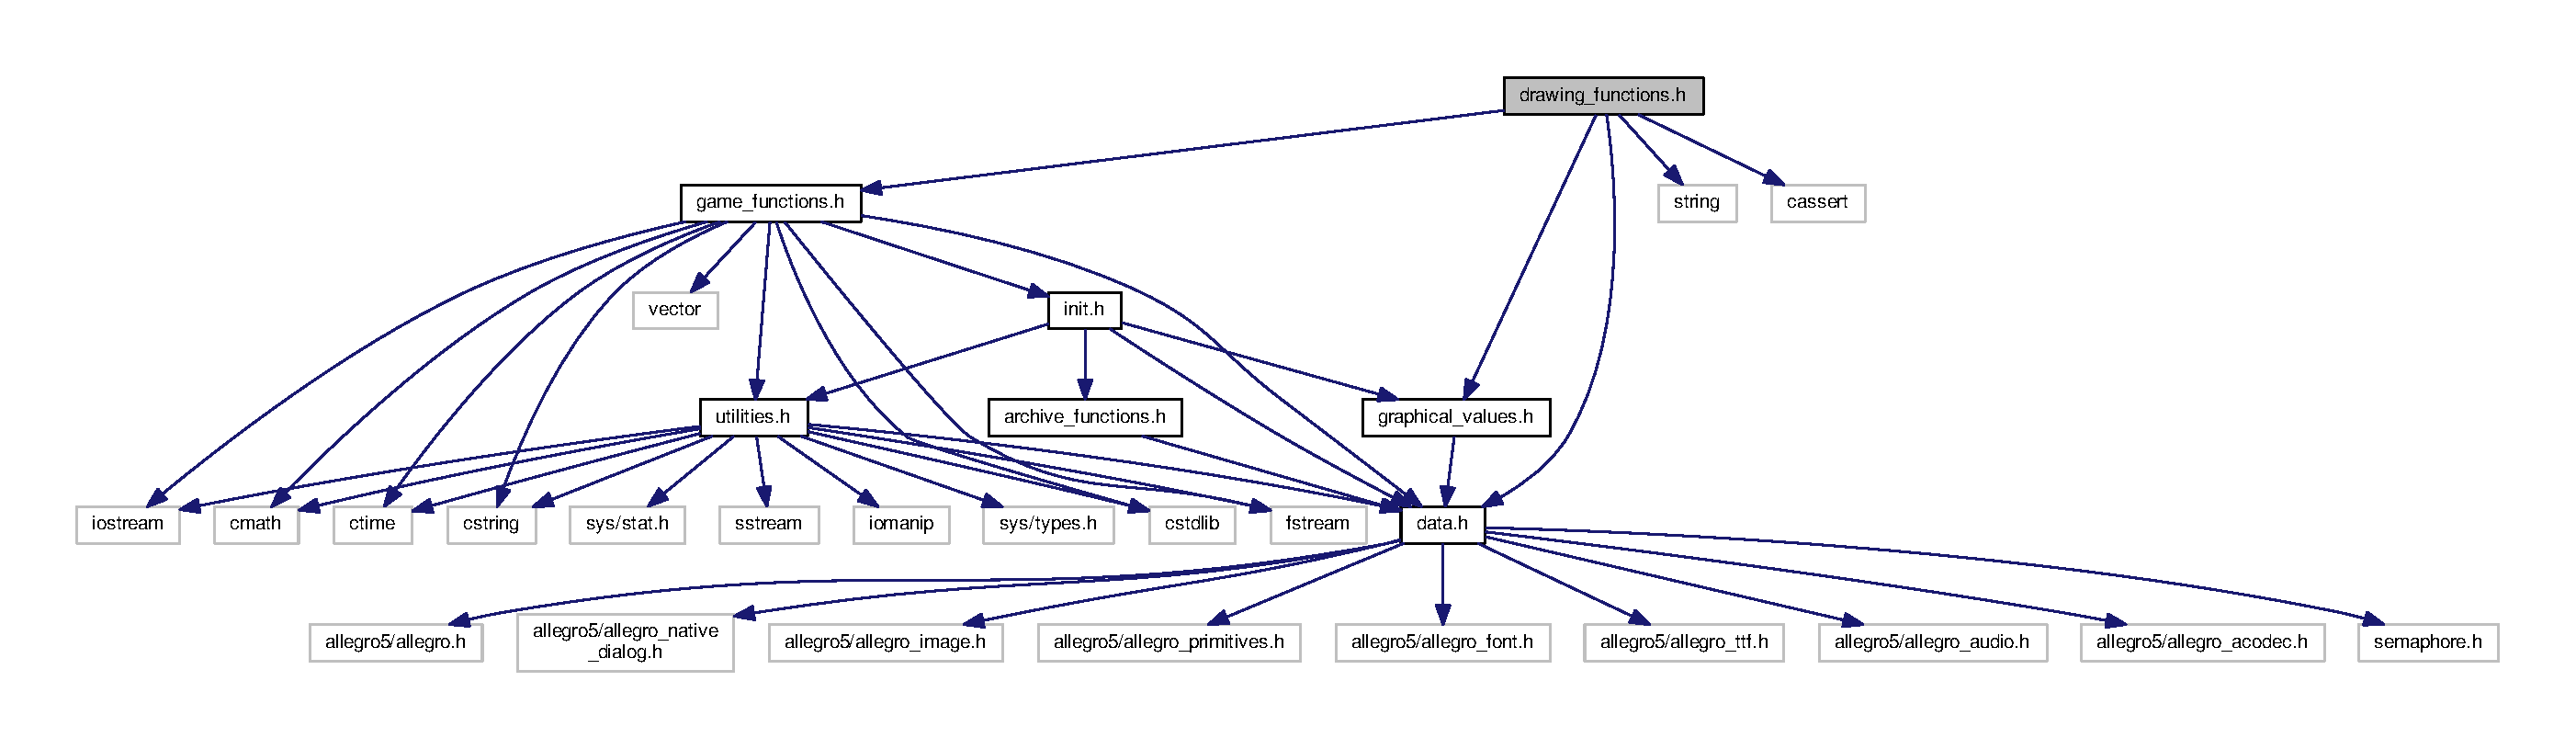
\includegraphics[width=350pt]{d5/d9c/drawing__functions_8h__incl}
\end{center}
\end{figure}
Questo grafo mostra quali altri file includono direttamente o indirettamente questo file\+:\nopagebreak
\begin{figure}[H]
\begin{center}
\leavevmode
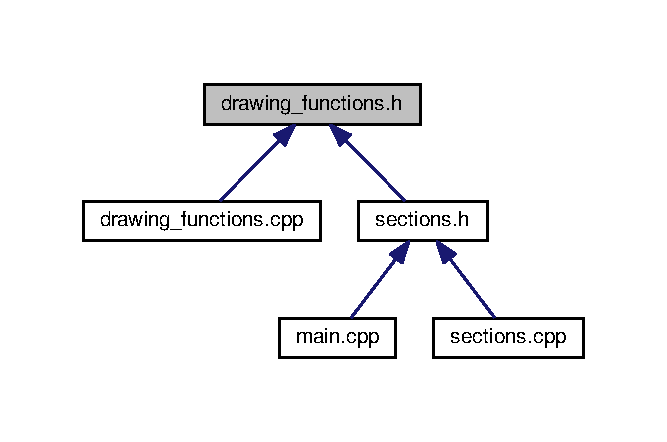
\includegraphics[width=320pt]{d2/d89/drawing__functions_8h__dep__incl}
\end{center}
\end{figure}
\subsection*{Funzioni}
\begin{DoxyCompactItemize}
\item 
A\+L\+L\+E\+G\+R\+O\+\_\+\+B\+I\+T\+M\+AP $\ast$$\ast$ \hyperlink{drawing__functions_8h_acaa107eaf4d6d8e1e1675d3e7c576277}{generate\+\_\+playwa\+\_\+bitmaps} ()
\begin{DoxyCompactList}\small\item\em Funzione che genera l\textquotesingle{}array contenente i puntatori ai bitmap relativi alla schermata di gioco. \end{DoxyCompactList}\item 
A\+L\+L\+E\+G\+R\+O\+\_\+\+F\+O\+NT $\ast$$\ast$ \hyperlink{drawing__functions_8h_a73982fb9ed5faaa34dd83cec1c8deb7c}{generate\+\_\+playwa\+\_\+fonts} ()
\begin{DoxyCompactList}\small\item\em Funzione che genera l\textquotesingle{}array contenente i puntatori ai font relativi alla schermata di gioco. \end{DoxyCompactList}\item 
A\+L\+L\+E\+G\+R\+O\+\_\+\+B\+I\+T\+M\+AP $\ast$$\ast$ \hyperlink{drawing__functions_8h_a4c5bc668d5d515156097d50ad1ea094c}{generate\+\_\+menu\+\_\+bitmaps} ()
\begin{DoxyCompactList}\small\item\em Funzione che genera l\textquotesingle{}array contenente i puntatori ai bitmap relativi alla schermata del menu principale. \end{DoxyCompactList}\item 
A\+L\+L\+E\+G\+R\+O\+\_\+\+B\+I\+T\+M\+AP $\ast$$\ast$ \hyperlink{drawing__functions_8h_a63f87e78d7d8340b2a5a02dc56b61718}{generate\+\_\+instr\+\_\+bitmaps} ()
\begin{DoxyCompactList}\small\item\em Funzione che genera l\textquotesingle{}array contenente i puntatori ai bitmap relativi alla schermata di pausa. \end{DoxyCompactList}\item 
A\+L\+L\+E\+G\+R\+O\+\_\+\+F\+O\+NT $\ast$$\ast$ \hyperlink{drawing__functions_8h_ac8a42fd07fd0472609d1334c696ca934}{generate\+\_\+menu\+\_\+fonts} ()
\begin{DoxyCompactList}\small\item\em Funzione che genera l\textquotesingle{}array contenente i puntatori ai font relativi ai menu. \end{DoxyCompactList}\item 
A\+L\+L\+E\+G\+R\+O\+\_\+\+F\+O\+NT $\ast$$\ast$ \hyperlink{drawing__functions_8h_a91ed375d606dbda8bdeaefde045bccc0}{generate\+\_\+instr\+\_\+fonts} ()
\begin{DoxyCompactList}\small\item\em Funzione che genera l\textquotesingle{}array contenente i puntatori ai font relativi alla schermata di pausa. \end{DoxyCompactList}\item 
A\+L\+L\+E\+G\+R\+O\+\_\+\+F\+O\+NT $\ast$$\ast$ \hyperlink{drawing__functions_8h_ae2818bfb00fa513611854338aeeef6ad}{generate\+\_\+user\+\_\+fonts} ()
\begin{DoxyCompactList}\small\item\em Funzione che genera l\textquotesingle{}array contenente i puntatori ai font relativi alla schermata di gameover. \end{DoxyCompactList}\item 
A\+L\+L\+E\+G\+R\+O\+\_\+\+F\+O\+NT $\ast$$\ast$ \hyperlink{drawing__functions_8h_ae4246ed2992a4852e394233e2b41d013}{generate\+\_\+settings\+\_\+fonts} ()
\begin{DoxyCompactList}\small\item\em Funzione che genera l\textquotesingle{}array contenente i puntatori ai font relativi alla schermata delle impostazioni. \end{DoxyCompactList}\item 
void \hyperlink{drawing__functions_8h_a30bcdca4f2bc932add7319374a3bb617}{destroy\+\_\+arr\+\_\+bitmaps} (A\+L\+L\+E\+G\+R\+O\+\_\+\+B\+I\+T\+M\+AP $\ast$$\ast$arr, const int num)
\begin{DoxyCompactList}\small\item\em Funzione che dealloca un array di bitmap, oltre che tutti i bitmap in esso contenuti. \end{DoxyCompactList}\item 
void \hyperlink{drawing__functions_8h_a3c93cba6ceb2ca7188621e0112220c8c}{destroy\+\_\+arr\+\_\+fonts} (A\+L\+L\+E\+G\+R\+O\+\_\+\+F\+O\+NT $\ast$$\ast$arr, const int num)
\begin{DoxyCompactList}\small\item\em Funzione che dealloca un array di font, oltre che tutti i font in esso contenuti. \end{DoxyCompactList}\item 
void \hyperlink{drawing__functions_8h_ae6b0d0c9d9a687608caf2b5f240758cf}{draw\+\_\+background} (A\+L\+L\+E\+G\+R\+O\+\_\+\+B\+I\+T\+M\+AP $\ast$bmp\+\_\+bg, float \&offset\+\_\+bg, const bool playing)
\begin{DoxyCompactList}\small\item\em Funzione che stampa lo sfondo della schermata. \end{DoxyCompactList}\item 
void \hyperlink{drawing__functions_8h_a1fc8105c4e2716aff11b7f1835be51b9}{draw\+\_\+head} (char $\ast$head\+\_\+str, A\+L\+L\+E\+G\+R\+O\+\_\+\+F\+O\+NT $\ast$font)
\begin{DoxyCompactList}\small\item\em Funzione che stampa il titolo della schermata. \end{DoxyCompactList}\item 
void \hyperlink{drawing__functions_8h_a5492eb7b0241c0d2cc97cda425addebd}{draw\+\_\+back} (A\+L\+L\+E\+G\+R\+O\+\_\+\+F\+O\+NT $\ast$font, const bool pause)
\begin{DoxyCompactList}\small\item\em Funzione che stampa la stringa di ritorno al gioco, o al menu principale (in base alla variabile \char`\"{}pause\char`\"{}). \end{DoxyCompactList}\item 
void \hyperlink{drawing__functions_8h_a497ccfc6d0c0bf91883fa091a8fc9310}{draw\+\_\+intro\+\_\+init} (A\+L\+L\+E\+G\+R\+O\+\_\+\+B\+I\+T\+M\+AP $\ast$$\ast$arr\+\_\+bitmaps, float \&bg\+\_\+offset)
\begin{DoxyCompactList}\small\item\em Funzione che gestisce l\textquotesingle{}inizializzazione dell\textquotesingle{}animazione di introduzione. \end{DoxyCompactList}\item 
void \hyperlink{drawing__functions_8h_adc09c13b7ec3fb805900982610c49cf9}{draw\+\_\+intro\+\_\+title\+\_\+slide} (A\+L\+L\+E\+G\+R\+O\+\_\+\+B\+I\+T\+M\+AP $\ast$$\ast$arr\+\_\+bitmaps, float \&bg\+\_\+offset)
\begin{DoxyCompactList}\small\item\em Funzione che gestisce lo slide del titolo nell\textquotesingle{}animazione di introduzione. \end{DoxyCompactList}\item 
void \hyperlink{drawing__functions_8h_a51a2880bf7e514344ee1ac5e562f9479}{draw\+\_\+intro\+\_\+menu\+\_\+fadein} (A\+L\+L\+E\+G\+R\+O\+\_\+\+B\+I\+T\+M\+AP $\ast$$\ast$arr\+\_\+bitmaps, A\+L\+L\+E\+G\+R\+O\+\_\+\+F\+O\+NT $\ast$$\ast$arr\+\_\+fonts, float \&bg\+\_\+offset)
\begin{DoxyCompactList}\small\item\em Funzione che gestisce il fadein del menu nell\textquotesingle{}animazione di introduzione. \end{DoxyCompactList}\item 
void \hyperlink{drawing__functions_8h_a9affe6a634fbf578ab2158cb6ae5ae7f}{draw\+\_\+menu\+\_\+title} (A\+L\+L\+E\+G\+R\+O\+\_\+\+B\+I\+T\+M\+AP $\ast$bmp\+\_\+title)
\begin{DoxyCompactList}\small\item\em Funzione che stampa il bitmap relativo al titolo presente nel menu principale. \end{DoxyCompactList}\item 
void \hyperlink{drawing__functions_8h_a9ce95bf12fc8789ae26027859ee5f47d}{draw\+\_\+menu\+\_\+option} (const int \&index, A\+L\+L\+E\+G\+R\+O\+\_\+\+B\+I\+T\+M\+AP $\ast$bmp\+\_\+option, A\+L\+L\+E\+G\+R\+O\+\_\+\+F\+O\+NT $\ast$font, char $\ast$str\+\_\+scelta, const bool settings)
\begin{DoxyCompactList}\small\item\em Funzione che stampa l\textquotesingle{}opzione indicata (menu). \end{DoxyCompactList}\item 
void \hyperlink{drawing__functions_8h_aa6d5deb3a6b2e9f1a2db69ff00badcbb}{draw\+\_\+menu\+\_\+copyright} (A\+L\+L\+E\+G\+R\+O\+\_\+\+F\+O\+NT $\ast$font)
\begin{DoxyCompactList}\small\item\em Funzione che stampa la stringa di copyright (menu). \end{DoxyCompactList}\item 
void \hyperlink{drawing__functions_8h_afcf3a6ebbfad9889b2b58b85f82814c7}{draw\+\_\+playwa\+\_\+score\+\_\+hint} (const \hyperlink{structmatch__vars__t}{match\+\_\+vars\+\_\+t} \&match\+\_\+vars, A\+L\+L\+E\+G\+R\+O\+\_\+\+F\+O\+NT $\ast$font\+\_\+score, A\+L\+L\+E\+G\+R\+O\+\_\+\+F\+O\+NT $\ast$font\+\_\+hints, const bool visible\+\_\+hints)
\begin{DoxyCompactList}\small\item\em Funzione che stampa il punteggio e i suggerimenti (schermata di gioco). \end{DoxyCompactList}\item 
void \hyperlink{drawing__functions_8h_aa12cd18d497401592c40fd5f803ed384}{draw\+\_\+playwa\+\_\+shooter} (const \hyperlink{structmatch__vars__t}{match\+\_\+vars\+\_\+t} \&match\+\_\+vars, const \hyperlink{structbullet__t}{bullet\+\_\+t} $\ast$arr\+\_\+bullet, const \hyperlink{structshooter__t}{shooter\+\_\+t} \&shooter, A\+L\+L\+E\+G\+R\+O\+\_\+\+B\+I\+T\+M\+AP $\ast$$\ast$arr\+\_\+bitmaps)
\begin{DoxyCompactList}\small\item\em Funzione che stampa lo shooter, la sua area (bianca normalmente, rossa in caso di pericolo o azzurra nel caso in cui il bonus \char`\"{}shield\char`\"{} venga attivato). \end{DoxyCompactList}\item 
void \hyperlink{drawing__functions_8h_a61d883b04452e38f3c290857d66941d7}{draw\+\_\+playwa\+\_\+asteroids\+\_\+bullets} (const \hyperlink{structmatch__vars__t}{match\+\_\+vars\+\_\+t} \&match\+\_\+vars, const \hyperlink{structbullet__t}{bullet\+\_\+t} $\ast$arr\+\_\+bullet, A\+L\+L\+E\+G\+R\+O\+\_\+\+B\+I\+T\+M\+AP $\ast$$\ast$arr\+\_\+bitmaps, A\+L\+L\+E\+G\+R\+O\+\_\+\+F\+O\+NT $\ast$font)
\begin{DoxyCompactList}\small\item\em Funzione che stampa lo gli asteroidi ed i proiettili presenti in gioco. \end{DoxyCompactList}\item 
void \hyperlink{drawing__functions_8h_acac0972652d8d16bcebdc571bd69d7cc}{draw\+\_\+playwa\+\_\+bonus\+\_\+music} (const \hyperlink{structmatch__vars__t}{match\+\_\+vars\+\_\+t} \&match\+\_\+vars, A\+L\+L\+E\+G\+R\+O\+\_\+\+B\+I\+T\+M\+AP $\ast$$\ast$arr\+\_\+bitmaps, A\+L\+L\+E\+G\+R\+O\+\_\+\+F\+O\+NT $\ast$font\+\_\+score, A\+L\+L\+E\+G\+R\+O\+\_\+\+F\+O\+NT $\ast$font\+\_\+bonus, A\+L\+L\+E\+G\+R\+O\+\_\+\+F\+O\+NT $\ast$font\+\_\+bonus\+\_\+hint, \hyperlink{structsettings__t}{settings\+\_\+t} settings)
\begin{DoxyCompactList}\small\item\em Funzione che stampa i bonus della partita (e le icone relative al suono). \end{DoxyCompactList}\item 
void \hyperlink{drawing__functions_8h_a05c0e4929a232f4cdcfbf43b05c79b39}{draw\+\_\+gameover\+\_\+animation} (const int \&score\+\_\+goal, const int \&dast\+\_\+goal, A\+L\+L\+E\+G\+R\+O\+\_\+\+B\+I\+T\+M\+AP $\ast$bg\+\_\+bmp, float \&bg\+\_\+offset, A\+L\+L\+E\+G\+R\+O\+\_\+\+F\+O\+NT $\ast$$\ast$arr\+\_\+fonts)
\begin{DoxyCompactList}\small\item\em Funzione che gestisce l\textquotesingle{}animazione di fine partita. \end{DoxyCompactList}\item 
void \hyperlink{drawing__functions_8h_ada8f618047616bdecf221bf0548fd2e5}{draw\+\_\+results} (A\+L\+L\+E\+G\+R\+O\+\_\+\+F\+O\+NT $\ast$font, \hyperlink{structresult__t}{result\+\_\+t} res)
\begin{DoxyCompactList}\small\item\em Funzione che disegna i risultati estratti dagli archivi corrispondenti alla password inserita dell\textquotesingle{}utente. \end{DoxyCompactList}\item 
void \hyperlink{drawing__functions_8h_ad713eae96f263309068c67fe145b9748}{draw\+\_\+playagain\+\_\+button} (A\+L\+L\+E\+G\+R\+O\+\_\+\+F\+O\+NT $\ast$font)
\begin{DoxyCompactList}\small\item\em Funzione che disegna il bottone \char`\"{}play again\char`\"{} nella schermata di Game Over. \end{DoxyCompactList}\item 
void \hyperlink{drawing__functions_8h_a3bf614e725835505499415b255bff0e7}{draw\+\_\+stats\+\_\+blocks} (A\+L\+L\+E\+G\+R\+O\+\_\+\+F\+O\+NT $\ast$font)
\begin{DoxyCompactList}\small\item\em Funzione che disegna i blocchi di sfondo relativi ai risultati di fine partita. \end{DoxyCompactList}\item 
void \hyperlink{drawing__functions_8h_a7f0ecbefa0f7f7cb274e8d5b56c3aa74}{draw\+\_\+stat} (const int \&idx\+\_\+stat, int stat\+\_\+value, A\+L\+L\+E\+G\+R\+O\+\_\+\+F\+O\+NT $\ast$font)
\begin{DoxyCompactList}\small\item\em Funzione che disegna un singolo risultato. \end{DoxyCompactList}\item 
void \hyperlink{drawing__functions_8h_acf0b8be217a189ac8895e0a879931602}{draw\+\_\+username\+\_\+block} (const bool enter\+\_\+active, A\+L\+L\+E\+G\+R\+O\+\_\+\+F\+O\+NT $\ast$font)
\begin{DoxyCompactList}\small\item\em Funzione che disegna il blocco di inserimento dello username. \end{DoxyCompactList}\item 
void \hyperlink{drawing__functions_8h_a6d58b45f3a62d5d1fd44a26e3e206c72}{draw\+\_\+username} (char $\ast$username, const int \&cur\+\_\+pos, A\+L\+L\+E\+G\+R\+O\+\_\+\+F\+O\+NT $\ast$font, const bool bar\+\_\+visible)
\begin{DoxyCompactList}\small\item\em Funzione che disegna lo username. \end{DoxyCompactList}\item 
void \hyperlink{drawing__functions_8h_a7b076accc9ae9e5e8e5e172d9bc50e8f}{draw\+\_\+instructions} (A\+L\+L\+E\+G\+R\+O\+\_\+\+F\+O\+NT $\ast$$\ast$arr\+\_\+fonts, A\+L\+L\+E\+G\+R\+O\+\_\+\+B\+I\+T\+M\+AP $\ast$$\ast$arr\+\_\+bitmaps)
\begin{DoxyCompactList}\small\item\em Funzine che disegna le istruzioni durante la pausa. \end{DoxyCompactList}\end{DoxyCompactItemize}
\subsection*{Variabili}
\begin{DoxyCompactItemize}
\item 
\hyperlink{structdisplay__info__t}{display\+\_\+info\+\_\+t} \hyperlink{drawing__functions_8h_a781a8df874545e4f5bff5f8a446d1963}{display\+\_\+info}
\item 
\hyperlink{structgeneral__gv__t}{general\+\_\+gv\+\_\+t} \hyperlink{drawing__functions_8h_aed9b611f5dc23d0c4b3423958ac92497}{G\+E\+N\+E\+R\+A\+L\+\_\+\+GV}
\begin{DoxyCompactList}\small\item\em Struct contenente le proporzioni grafiche generali. \end{DoxyCompactList}\item 
\hyperlink{structmenu__gv__t}{menu\+\_\+gv\+\_\+t} \hyperlink{drawing__functions_8h_a8050b794d70ca38807298569dc1af9b1}{M\+E\+N\+U\+\_\+\+GV}
\begin{DoxyCompactList}\small\item\em Struct contenente le proporzioni grafiche dei menu. \end{DoxyCompactList}\item 
\hyperlink{structplaywa__gv__t}{playwa\+\_\+gv\+\_\+t} \hyperlink{drawing__functions_8h_a38bfadb0325688402bf1999301ca2a1b}{P\+L\+A\+Y\+W\+A\+\_\+\+GV}
\begin{DoxyCompactList}\small\item\em Struct contenente le proporzioni grafiche della schermata di gioco. \end{DoxyCompactList}\item 
\hyperlink{structinstr__gv__t}{instr\+\_\+gv\+\_\+t} \hyperlink{drawing__functions_8h_a19a4da312ef3ea2a005acbce135d96fd}{I\+N\+S\+T\+R\+\_\+\+GV}
\begin{DoxyCompactList}\small\item\em Struct contenente le proporzioni grafiche della schermata di pausa. \end{DoxyCompactList}\item 
\hyperlink{structusr__gv__t}{usr\+\_\+gv\+\_\+t} \hyperlink{drawing__functions_8h_aba4a0deff6c9de510c6621913ab2a406}{U\+S\+R\+\_\+\+GV}
\begin{DoxyCompactList}\small\item\em Struct contenente le proporzioni grafiche della schermata di fine partita. \end{DoxyCompactList}\end{DoxyCompactItemize}


\subsection{Documentazione delle funzioni}
\mbox{\Hypertarget{drawing__functions_8h_a30bcdca4f2bc932add7319374a3bb617}\label{drawing__functions_8h_a30bcdca4f2bc932add7319374a3bb617}} 
\index{drawing\+\_\+functions.\+h@{drawing\+\_\+functions.\+h}!destroy\+\_\+arr\+\_\+bitmaps@{destroy\+\_\+arr\+\_\+bitmaps}}
\index{destroy\+\_\+arr\+\_\+bitmaps@{destroy\+\_\+arr\+\_\+bitmaps}!drawing\+\_\+functions.\+h@{drawing\+\_\+functions.\+h}}
\subsubsection{\texorpdfstring{destroy\+\_\+arr\+\_\+bitmaps()}{destroy\_arr\_bitmaps()}}
{\footnotesize\ttfamily void destroy\+\_\+arr\+\_\+bitmaps (\begin{DoxyParamCaption}\item[{A\+L\+L\+E\+G\+R\+O\+\_\+\+B\+I\+T\+M\+AP $\ast$$\ast$}]{arr,  }\item[{const int}]{num }\end{DoxyParamCaption})}



Funzione che dealloca un array di bitmap, oltre che tutti i bitmap in esso contenuti. 

~\newline
Parametri\+: ~\newline
1) arr -\/ Array di bitmap; ~\newline
2) num -\/ Dimensione dell\textquotesingle{}array di bitmap. \mbox{\Hypertarget{drawing__functions_8h_a3c93cba6ceb2ca7188621e0112220c8c}\label{drawing__functions_8h_a3c93cba6ceb2ca7188621e0112220c8c}} 
\index{drawing\+\_\+functions.\+h@{drawing\+\_\+functions.\+h}!destroy\+\_\+arr\+\_\+fonts@{destroy\+\_\+arr\+\_\+fonts}}
\index{destroy\+\_\+arr\+\_\+fonts@{destroy\+\_\+arr\+\_\+fonts}!drawing\+\_\+functions.\+h@{drawing\+\_\+functions.\+h}}
\subsubsection{\texorpdfstring{destroy\+\_\+arr\+\_\+fonts()}{destroy\_arr\_fonts()}}
{\footnotesize\ttfamily void destroy\+\_\+arr\+\_\+fonts (\begin{DoxyParamCaption}\item[{A\+L\+L\+E\+G\+R\+O\+\_\+\+F\+O\+NT $\ast$$\ast$}]{arr,  }\item[{const int}]{num }\end{DoxyParamCaption})}



Funzione che dealloca un array di font, oltre che tutti i font in esso contenuti. 

~\newline
Parametri\+: ~\newline
1) arr -\/ Array di font; ~\newline
2) num -\/ Dimensione dell\textquotesingle{}array di font. \mbox{\Hypertarget{drawing__functions_8h_a5492eb7b0241c0d2cc97cda425addebd}\label{drawing__functions_8h_a5492eb7b0241c0d2cc97cda425addebd}} 
\index{drawing\+\_\+functions.\+h@{drawing\+\_\+functions.\+h}!draw\+\_\+back@{draw\+\_\+back}}
\index{draw\+\_\+back@{draw\+\_\+back}!drawing\+\_\+functions.\+h@{drawing\+\_\+functions.\+h}}
\subsubsection{\texorpdfstring{draw\+\_\+back()}{draw\_back()}}
{\footnotesize\ttfamily void draw\+\_\+back (\begin{DoxyParamCaption}\item[{A\+L\+L\+E\+G\+R\+O\+\_\+\+F\+O\+NT $\ast$}]{font,  }\item[{const bool}]{pause }\end{DoxyParamCaption})}



Funzione che stampa la stringa di ritorno al gioco, o al menu principale (in base alla variabile \char`\"{}pause\char`\"{}). 

~\newline
Parametri\+: ~\newline
1) font -\/ Font relativo alla stringa di ritorno; ~\newline
2) pause -\/ In base al valore assunto da questa variabile viene stampata la stringa adatta. \mbox{\Hypertarget{drawing__functions_8h_ae6b0d0c9d9a687608caf2b5f240758cf}\label{drawing__functions_8h_ae6b0d0c9d9a687608caf2b5f240758cf}} 
\index{drawing\+\_\+functions.\+h@{drawing\+\_\+functions.\+h}!draw\+\_\+background@{draw\+\_\+background}}
\index{draw\+\_\+background@{draw\+\_\+background}!drawing\+\_\+functions.\+h@{drawing\+\_\+functions.\+h}}
\subsubsection{\texorpdfstring{draw\+\_\+background()}{draw\_background()}}
{\footnotesize\ttfamily void draw\+\_\+background (\begin{DoxyParamCaption}\item[{A\+L\+L\+E\+G\+R\+O\+\_\+\+B\+I\+T\+M\+AP $\ast$}]{bmp\+\_\+bg,  }\item[{float \&}]{offset\+\_\+bg,  }\item[{const bool}]{playing }\end{DoxyParamCaption})}



Funzione che stampa lo sfondo della schermata. 

~\newline
Parametri\+: ~\newline
1) bmp\+\_\+bg -\/ Bitmap relativo allo sfondo; ~\newline
2) offset\+\_\+bg -\/ Scostamento in pixel dello sfondo dal lato sinistro della schermata (per rotazione sfondo); ~\newline
3) playing -\/ Flag sul quale si basa la velocità di rotazione (durante il gioco risulta essere più lenta). \mbox{\Hypertarget{drawing__functions_8h_a05c0e4929a232f4cdcfbf43b05c79b39}\label{drawing__functions_8h_a05c0e4929a232f4cdcfbf43b05c79b39}} 
\index{drawing\+\_\+functions.\+h@{drawing\+\_\+functions.\+h}!draw\+\_\+gameover\+\_\+animation@{draw\+\_\+gameover\+\_\+animation}}
\index{draw\+\_\+gameover\+\_\+animation@{draw\+\_\+gameover\+\_\+animation}!drawing\+\_\+functions.\+h@{drawing\+\_\+functions.\+h}}
\subsubsection{\texorpdfstring{draw\+\_\+gameover\+\_\+animation()}{draw\_gameover\_animation()}}
{\footnotesize\ttfamily void draw\+\_\+gameover\+\_\+animation (\begin{DoxyParamCaption}\item[{const int \&}]{score\+\_\+goal,  }\item[{const int \&}]{dast\+\_\+goal,  }\item[{A\+L\+L\+E\+G\+R\+O\+\_\+\+B\+I\+T\+M\+AP $\ast$}]{bg\+\_\+bmp,  }\item[{float \&}]{bg\+\_\+offset,  }\item[{A\+L\+L\+E\+G\+R\+O\+\_\+\+F\+O\+NT $\ast$$\ast$}]{arr\+\_\+fonts }\end{DoxyParamCaption})}



Funzione che gestisce l\textquotesingle{}animazione di fine partita. 

~\newline
Parametri\+: ~\newline
1) score\+\_\+goal -\/ Score effettiva del giocatore; ~\newline
2) dast\+\_\+goal -\/ Asteroidi effettivamente distrutti; ~\newline
4) bg\+\_\+bmp -\/ Bitmap di sfondo; ~\newline
5) bg\+\_\+offset -\/ Scostamento laterale dello sfondo; ~\newline
6) arr\+\_\+fonts -\/ Array dei font necessari. \mbox{\Hypertarget{drawing__functions_8h_a1fc8105c4e2716aff11b7f1835be51b9}\label{drawing__functions_8h_a1fc8105c4e2716aff11b7f1835be51b9}} 
\index{drawing\+\_\+functions.\+h@{drawing\+\_\+functions.\+h}!draw\+\_\+head@{draw\+\_\+head}}
\index{draw\+\_\+head@{draw\+\_\+head}!drawing\+\_\+functions.\+h@{drawing\+\_\+functions.\+h}}
\subsubsection{\texorpdfstring{draw\+\_\+head()}{draw\_head()}}
{\footnotesize\ttfamily void draw\+\_\+head (\begin{DoxyParamCaption}\item[{char $\ast$}]{head\+\_\+str,  }\item[{A\+L\+L\+E\+G\+R\+O\+\_\+\+F\+O\+NT $\ast$}]{font }\end{DoxyParamCaption})}



Funzione che stampa il titolo della schermata. 

~\newline
Parametri\+: ~\newline
1) head\+\_\+str -\/ Stringa relativa al titolo; ~\newline
2) font -\/ Font relativo al titolo. \mbox{\Hypertarget{drawing__functions_8h_a7b076accc9ae9e5e8e5e172d9bc50e8f}\label{drawing__functions_8h_a7b076accc9ae9e5e8e5e172d9bc50e8f}} 
\index{drawing\+\_\+functions.\+h@{drawing\+\_\+functions.\+h}!draw\+\_\+instructions@{draw\+\_\+instructions}}
\index{draw\+\_\+instructions@{draw\+\_\+instructions}!drawing\+\_\+functions.\+h@{drawing\+\_\+functions.\+h}}
\subsubsection{\texorpdfstring{draw\+\_\+instructions()}{draw\_instructions()}}
{\footnotesize\ttfamily void draw\+\_\+instructions (\begin{DoxyParamCaption}\item[{A\+L\+L\+E\+G\+R\+O\+\_\+\+F\+O\+NT $\ast$$\ast$}]{arr\+\_\+fonts,  }\item[{A\+L\+L\+E\+G\+R\+O\+\_\+\+B\+I\+T\+M\+AP $\ast$$\ast$}]{arr\+\_\+bitmaps }\end{DoxyParamCaption})}



Funzine che disegna le istruzioni durante la pausa. 

~\newline
Parametri\+: ~\newline
1) arr\+\_\+fonts -\/ Array contenente i font utilizzati; ~\newline
2) arr\+\_\+bitmaps -\/ Array contenente i bitmap utilizzati. \mbox{\Hypertarget{drawing__functions_8h_a497ccfc6d0c0bf91883fa091a8fc9310}\label{drawing__functions_8h_a497ccfc6d0c0bf91883fa091a8fc9310}} 
\index{drawing\+\_\+functions.\+h@{drawing\+\_\+functions.\+h}!draw\+\_\+intro\+\_\+init@{draw\+\_\+intro\+\_\+init}}
\index{draw\+\_\+intro\+\_\+init@{draw\+\_\+intro\+\_\+init}!drawing\+\_\+functions.\+h@{drawing\+\_\+functions.\+h}}
\subsubsection{\texorpdfstring{draw\+\_\+intro\+\_\+init()}{draw\_intro\_init()}}
{\footnotesize\ttfamily void draw\+\_\+intro\+\_\+init (\begin{DoxyParamCaption}\item[{A\+L\+L\+E\+G\+R\+O\+\_\+\+B\+I\+T\+M\+AP $\ast$$\ast$}]{arr\+\_\+bitmaps,  }\item[{float \&}]{bg\+\_\+offset }\end{DoxyParamCaption})}



Funzione che gestisce l\textquotesingle{}inizializzazione dell\textquotesingle{}animazione di introduzione. 

~\newline
Parametri\+: ~\newline
1) arr\+\_\+bitmaps -\/ Array di bitmap; ~\newline
2) bg\+\_\+offset -\/ Offset iniziale dello sfondo. \mbox{\Hypertarget{drawing__functions_8h_a51a2880bf7e514344ee1ac5e562f9479}\label{drawing__functions_8h_a51a2880bf7e514344ee1ac5e562f9479}} 
\index{drawing\+\_\+functions.\+h@{drawing\+\_\+functions.\+h}!draw\+\_\+intro\+\_\+menu\+\_\+fadein@{draw\+\_\+intro\+\_\+menu\+\_\+fadein}}
\index{draw\+\_\+intro\+\_\+menu\+\_\+fadein@{draw\+\_\+intro\+\_\+menu\+\_\+fadein}!drawing\+\_\+functions.\+h@{drawing\+\_\+functions.\+h}}
\subsubsection{\texorpdfstring{draw\+\_\+intro\+\_\+menu\+\_\+fadein()}{draw\_intro\_menu\_fadein()}}
{\footnotesize\ttfamily void draw\+\_\+intro\+\_\+menu\+\_\+fadein (\begin{DoxyParamCaption}\item[{A\+L\+L\+E\+G\+R\+O\+\_\+\+B\+I\+T\+M\+AP $\ast$$\ast$}]{arr\+\_\+bitmaps,  }\item[{A\+L\+L\+E\+G\+R\+O\+\_\+\+F\+O\+NT $\ast$$\ast$}]{arr\+\_\+fonts,  }\item[{float \&}]{bg\+\_\+offset }\end{DoxyParamCaption})}



Funzione che gestisce il fadein del menu nell\textquotesingle{}animazione di introduzione. 

~\newline
Parametri\+: ~\newline
1) arr\+\_\+bitmaps -\/ Array di bitmap; ~\newline
2) arr\+\_\+fonts -\/ Array di font; ~\newline
3) bg\+\_\+offset -\/ Offset iniziale dello sfondo. \mbox{\Hypertarget{drawing__functions_8h_adc09c13b7ec3fb805900982610c49cf9}\label{drawing__functions_8h_adc09c13b7ec3fb805900982610c49cf9}} 
\index{drawing\+\_\+functions.\+h@{drawing\+\_\+functions.\+h}!draw\+\_\+intro\+\_\+title\+\_\+slide@{draw\+\_\+intro\+\_\+title\+\_\+slide}}
\index{draw\+\_\+intro\+\_\+title\+\_\+slide@{draw\+\_\+intro\+\_\+title\+\_\+slide}!drawing\+\_\+functions.\+h@{drawing\+\_\+functions.\+h}}
\subsubsection{\texorpdfstring{draw\+\_\+intro\+\_\+title\+\_\+slide()}{draw\_intro\_title\_slide()}}
{\footnotesize\ttfamily void draw\+\_\+intro\+\_\+title\+\_\+slide (\begin{DoxyParamCaption}\item[{A\+L\+L\+E\+G\+R\+O\+\_\+\+B\+I\+T\+M\+AP $\ast$$\ast$}]{arr\+\_\+bitmaps,  }\item[{float \&}]{bg\+\_\+offset }\end{DoxyParamCaption})}



Funzione che gestisce lo slide del titolo nell\textquotesingle{}animazione di introduzione. 

~\newline
Parametri\+: ~\newline
1) arr\+\_\+bitmaps -\/ Array di bitmap; ~\newline
2) bg\+\_\+offset -\/ Offset iniziale dello sfondo. \mbox{\Hypertarget{drawing__functions_8h_aa6d5deb3a6b2e9f1a2db69ff00badcbb}\label{drawing__functions_8h_aa6d5deb3a6b2e9f1a2db69ff00badcbb}} 
\index{drawing\+\_\+functions.\+h@{drawing\+\_\+functions.\+h}!draw\+\_\+menu\+\_\+copyright@{draw\+\_\+menu\+\_\+copyright}}
\index{draw\+\_\+menu\+\_\+copyright@{draw\+\_\+menu\+\_\+copyright}!drawing\+\_\+functions.\+h@{drawing\+\_\+functions.\+h}}
\subsubsection{\texorpdfstring{draw\+\_\+menu\+\_\+copyright()}{draw\_menu\_copyright()}}
{\footnotesize\ttfamily void draw\+\_\+menu\+\_\+copyright (\begin{DoxyParamCaption}\item[{A\+L\+L\+E\+G\+R\+O\+\_\+\+F\+O\+NT $\ast$}]{font }\end{DoxyParamCaption})}



Funzione che stampa la stringa di copyright (menu). 

~\newline
Parametri\+: ~\newline
1) font -\/ Font relativo alla stringa di copyright. \mbox{\Hypertarget{drawing__functions_8h_a9ce95bf12fc8789ae26027859ee5f47d}\label{drawing__functions_8h_a9ce95bf12fc8789ae26027859ee5f47d}} 
\index{drawing\+\_\+functions.\+h@{drawing\+\_\+functions.\+h}!draw\+\_\+menu\+\_\+option@{draw\+\_\+menu\+\_\+option}}
\index{draw\+\_\+menu\+\_\+option@{draw\+\_\+menu\+\_\+option}!drawing\+\_\+functions.\+h@{drawing\+\_\+functions.\+h}}
\subsubsection{\texorpdfstring{draw\+\_\+menu\+\_\+option()}{draw\_menu\_option()}}
{\footnotesize\ttfamily void draw\+\_\+menu\+\_\+option (\begin{DoxyParamCaption}\item[{const int \&}]{index,  }\item[{A\+L\+L\+E\+G\+R\+O\+\_\+\+B\+I\+T\+M\+AP $\ast$}]{bmp\+\_\+option,  }\item[{A\+L\+L\+E\+G\+R\+O\+\_\+\+F\+O\+NT $\ast$}]{font,  }\item[{char $\ast$}]{str\+\_\+scelta,  }\item[{const bool}]{settings }\end{DoxyParamCaption})}



Funzione che stampa l\textquotesingle{}opzione indicata (menu). 

~\newline
Parametri\+: ~\newline
1) index -\/ Indice dell\textquotesingle{}opzione; ~\newline
2) bmp\+\_\+option -\/ Bitmap relativo all\textquotesingle{}opzione indicata; ~\newline
3) font -\/ Font relativo all\textquotesingle{}opzione indicata; ~\newline
4) str\+\_\+scelta -\/ Stringa relativa all\textquotesingle{}opzione indicata; ~\newline
5) settings -\/ Se vero, stampa le opzioni leggermente più in alto rispetto al menu principale. \mbox{\Hypertarget{drawing__functions_8h_a9affe6a634fbf578ab2158cb6ae5ae7f}\label{drawing__functions_8h_a9affe6a634fbf578ab2158cb6ae5ae7f}} 
\index{drawing\+\_\+functions.\+h@{drawing\+\_\+functions.\+h}!draw\+\_\+menu\+\_\+title@{draw\+\_\+menu\+\_\+title}}
\index{draw\+\_\+menu\+\_\+title@{draw\+\_\+menu\+\_\+title}!drawing\+\_\+functions.\+h@{drawing\+\_\+functions.\+h}}
\subsubsection{\texorpdfstring{draw\+\_\+menu\+\_\+title()}{draw\_menu\_title()}}
{\footnotesize\ttfamily void draw\+\_\+menu\+\_\+title (\begin{DoxyParamCaption}\item[{A\+L\+L\+E\+G\+R\+O\+\_\+\+B\+I\+T\+M\+AP $\ast$}]{bmp\+\_\+title }\end{DoxyParamCaption})}



Funzione che stampa il bitmap relativo al titolo presente nel menu principale. 

~\newline
Parametri\+: ~\newline
1) bmp\+\_\+title -\/ Bitmap relativo al titolo. \mbox{\Hypertarget{drawing__functions_8h_ad713eae96f263309068c67fe145b9748}\label{drawing__functions_8h_ad713eae96f263309068c67fe145b9748}} 
\index{drawing\+\_\+functions.\+h@{drawing\+\_\+functions.\+h}!draw\+\_\+playagain\+\_\+button@{draw\+\_\+playagain\+\_\+button}}
\index{draw\+\_\+playagain\+\_\+button@{draw\+\_\+playagain\+\_\+button}!drawing\+\_\+functions.\+h@{drawing\+\_\+functions.\+h}}
\subsubsection{\texorpdfstring{draw\+\_\+playagain\+\_\+button()}{draw\_playagain\_button()}}
{\footnotesize\ttfamily void draw\+\_\+playagain\+\_\+button (\begin{DoxyParamCaption}\item[{A\+L\+L\+E\+G\+R\+O\+\_\+\+F\+O\+NT $\ast$}]{font }\end{DoxyParamCaption})}



Funzione che disegna il bottone \char`\"{}play again\char`\"{} nella schermata di Game Over. 

~\newline
Parametri\+: ~\newline
1) arr\+\_\+fonts -\/ Array dei font necessari;~\newline
\mbox{\Hypertarget{drawing__functions_8h_a61d883b04452e38f3c290857d66941d7}\label{drawing__functions_8h_a61d883b04452e38f3c290857d66941d7}} 
\index{drawing\+\_\+functions.\+h@{drawing\+\_\+functions.\+h}!draw\+\_\+playwa\+\_\+asteroids\+\_\+bullets@{draw\+\_\+playwa\+\_\+asteroids\+\_\+bullets}}
\index{draw\+\_\+playwa\+\_\+asteroids\+\_\+bullets@{draw\+\_\+playwa\+\_\+asteroids\+\_\+bullets}!drawing\+\_\+functions.\+h@{drawing\+\_\+functions.\+h}}
\subsubsection{\texorpdfstring{draw\+\_\+playwa\+\_\+asteroids\+\_\+bullets()}{draw\_playwa\_asteroids\_bullets()}}
{\footnotesize\ttfamily void draw\+\_\+playwa\+\_\+asteroids\+\_\+bullets (\begin{DoxyParamCaption}\item[{const \hyperlink{structmatch__vars__t}{match\+\_\+vars\+\_\+t} \&}]{match\+\_\+vars,  }\item[{const \hyperlink{structbullet__t}{bullet\+\_\+t} $\ast$}]{arr\+\_\+bullet,  }\item[{A\+L\+L\+E\+G\+R\+O\+\_\+\+B\+I\+T\+M\+AP $\ast$$\ast$}]{arr\+\_\+bitmaps,  }\item[{A\+L\+L\+E\+G\+R\+O\+\_\+\+F\+O\+NT $\ast$}]{font }\end{DoxyParamCaption})}



Funzione che stampa lo gli asteroidi ed i proiettili presenti in gioco. 

~\newline
Parametri\+: ~\newline
1) match\+\_\+vars -\/ Struct contenente le variabili di gioco; ~\newline
2) arr\+\_\+bullet -\/ Array contenente i proiettili in gioco; ~\newline
3) arr\+\_\+bitmaps -\/ Array contenente i bitmap di gioco; ~\newline
4) font -\/ Font relativo agli asteroidi. \mbox{\Hypertarget{drawing__functions_8h_acac0972652d8d16bcebdc571bd69d7cc}\label{drawing__functions_8h_acac0972652d8d16bcebdc571bd69d7cc}} 
\index{drawing\+\_\+functions.\+h@{drawing\+\_\+functions.\+h}!draw\+\_\+playwa\+\_\+bonus\+\_\+music@{draw\+\_\+playwa\+\_\+bonus\+\_\+music}}
\index{draw\+\_\+playwa\+\_\+bonus\+\_\+music@{draw\+\_\+playwa\+\_\+bonus\+\_\+music}!drawing\+\_\+functions.\+h@{drawing\+\_\+functions.\+h}}
\subsubsection{\texorpdfstring{draw\+\_\+playwa\+\_\+bonus\+\_\+music()}{draw\_playwa\_bonus\_music()}}
{\footnotesize\ttfamily void draw\+\_\+playwa\+\_\+bonus\+\_\+music (\begin{DoxyParamCaption}\item[{const \hyperlink{structmatch__vars__t}{match\+\_\+vars\+\_\+t} \&}]{match\+\_\+vars,  }\item[{A\+L\+L\+E\+G\+R\+O\+\_\+\+B\+I\+T\+M\+AP $\ast$$\ast$}]{arr\+\_\+bitmaps,  }\item[{A\+L\+L\+E\+G\+R\+O\+\_\+\+F\+O\+NT $\ast$}]{font\+\_\+score,  }\item[{A\+L\+L\+E\+G\+R\+O\+\_\+\+F\+O\+NT $\ast$}]{font\+\_\+bonus,  }\item[{A\+L\+L\+E\+G\+R\+O\+\_\+\+F\+O\+NT $\ast$}]{font\+\_\+bonus\+\_\+hint,  }\item[{\hyperlink{structsettings__t}{settings\+\_\+t}}]{settings }\end{DoxyParamCaption})}



Funzione che stampa i bonus della partita (e le icone relative al suono). 

~\newline
Parametri\+: ~\newline
1) match\+\_\+vars -\/ Struct contenente le variabili di gioco; ~\newline
2) arr\+\_\+bitmaps -\/ Array contenente i bitmap di gioco; ~\newline
3) font\+\_\+score -\/ Font relativo al punteggio (utilizzato per stampare l\textquotesingle{}intestazione dei bonus); ~\newline
4) font\+\_\+bonus -\/ Font relativo alla numerosità dei bonus; ~\newline
5) font\+\_\+bonus\+\_\+hint -\/ Font relativo al suggerimento per l\textquotesingle{}attivazione del bonus. \mbox{\Hypertarget{drawing__functions_8h_afcf3a6ebbfad9889b2b58b85f82814c7}\label{drawing__functions_8h_afcf3a6ebbfad9889b2b58b85f82814c7}} 
\index{drawing\+\_\+functions.\+h@{drawing\+\_\+functions.\+h}!draw\+\_\+playwa\+\_\+score\+\_\+hint@{draw\+\_\+playwa\+\_\+score\+\_\+hint}}
\index{draw\+\_\+playwa\+\_\+score\+\_\+hint@{draw\+\_\+playwa\+\_\+score\+\_\+hint}!drawing\+\_\+functions.\+h@{drawing\+\_\+functions.\+h}}
\subsubsection{\texorpdfstring{draw\+\_\+playwa\+\_\+score\+\_\+hint()}{draw\_playwa\_score\_hint()}}
{\footnotesize\ttfamily void draw\+\_\+playwa\+\_\+score\+\_\+hint (\begin{DoxyParamCaption}\item[{const \hyperlink{structmatch__vars__t}{match\+\_\+vars\+\_\+t} \&}]{match\+\_\+vars,  }\item[{A\+L\+L\+E\+G\+R\+O\+\_\+\+F\+O\+NT $\ast$}]{font\+\_\+score,  }\item[{A\+L\+L\+E\+G\+R\+O\+\_\+\+F\+O\+NT $\ast$}]{font\+\_\+hints,  }\item[{const bool}]{visible\+\_\+hints }\end{DoxyParamCaption})}



Funzione che stampa il punteggio e i suggerimenti (schermata di gioco). 

~\newline
Parametri\+: ~\newline
1) match\+\_\+vars -\/ Struct contenente le variabili di gioco; ~\newline
2) font\+\_\+score -\/ Font relativo al punteggio; ~\newline
3) font\+\_\+hints -\/ Font relativo ai suggerimenti; ~\newline
4) visible\+\_\+hints -\/ Se true, mostra i suggerimenti di gioco. \mbox{\Hypertarget{drawing__functions_8h_aa12cd18d497401592c40fd5f803ed384}\label{drawing__functions_8h_aa12cd18d497401592c40fd5f803ed384}} 
\index{drawing\+\_\+functions.\+h@{drawing\+\_\+functions.\+h}!draw\+\_\+playwa\+\_\+shooter@{draw\+\_\+playwa\+\_\+shooter}}
\index{draw\+\_\+playwa\+\_\+shooter@{draw\+\_\+playwa\+\_\+shooter}!drawing\+\_\+functions.\+h@{drawing\+\_\+functions.\+h}}
\subsubsection{\texorpdfstring{draw\+\_\+playwa\+\_\+shooter()}{draw\_playwa\_shooter()}}
{\footnotesize\ttfamily void draw\+\_\+playwa\+\_\+shooter (\begin{DoxyParamCaption}\item[{const \hyperlink{structmatch__vars__t}{match\+\_\+vars\+\_\+t} \&}]{match\+\_\+vars,  }\item[{const \hyperlink{structbullet__t}{bullet\+\_\+t} $\ast$}]{arr\+\_\+bullet,  }\item[{const \hyperlink{structshooter__t}{shooter\+\_\+t} \&}]{shooter,  }\item[{A\+L\+L\+E\+G\+R\+O\+\_\+\+B\+I\+T\+M\+AP $\ast$$\ast$}]{arr\+\_\+bitmaps }\end{DoxyParamCaption})}



Funzione che stampa lo shooter, la sua area (bianca normalmente, rossa in caso di pericolo o azzurra nel caso in cui il bonus \char`\"{}shield\char`\"{} venga attivato). 

~\newline
Parametri\+: ~\newline
1) match\+\_\+vars -\/ Struct contenente le variabili di gioco; ~\newline
2) arr\+\_\+bullet -\/ Array contenente i proiettili in gioco; ~\newline
3) shooter -\/ Struct contenente le variabili relative allo shooter; ~\newline
4) arr\+\_\+bitmaps -\/ Array contenente i bitmap di gioco. \mbox{\Hypertarget{drawing__functions_8h_ada8f618047616bdecf221bf0548fd2e5}\label{drawing__functions_8h_ada8f618047616bdecf221bf0548fd2e5}} 
\index{drawing\+\_\+functions.\+h@{drawing\+\_\+functions.\+h}!draw\+\_\+results@{draw\+\_\+results}}
\index{draw\+\_\+results@{draw\+\_\+results}!drawing\+\_\+functions.\+h@{drawing\+\_\+functions.\+h}}
\subsubsection{\texorpdfstring{draw\+\_\+results()}{draw\_results()}}
{\footnotesize\ttfamily void draw\+\_\+results (\begin{DoxyParamCaption}\item[{A\+L\+L\+E\+G\+R\+O\+\_\+\+F\+O\+NT $\ast$}]{font,  }\item[{\hyperlink{structresult__t}{result\+\_\+t}}]{res }\end{DoxyParamCaption})}



Funzione che disegna i risultati estratti dagli archivi corrispondenti alla password inserita dell\textquotesingle{}utente. 

~\newline
Parametri\+: ~\newline
1) arr\+\_\+fonts -\/ Array dei font necessari;~\newline
2) res -\/ Risultati dei match estratti; \mbox{\Hypertarget{drawing__functions_8h_a7f0ecbefa0f7f7cb274e8d5b56c3aa74}\label{drawing__functions_8h_a7f0ecbefa0f7f7cb274e8d5b56c3aa74}} 
\index{drawing\+\_\+functions.\+h@{drawing\+\_\+functions.\+h}!draw\+\_\+stat@{draw\+\_\+stat}}
\index{draw\+\_\+stat@{draw\+\_\+stat}!drawing\+\_\+functions.\+h@{drawing\+\_\+functions.\+h}}
\subsubsection{\texorpdfstring{draw\+\_\+stat()}{draw\_stat()}}
{\footnotesize\ttfamily void draw\+\_\+stat (\begin{DoxyParamCaption}\item[{const int \&}]{idx\+\_\+stat,  }\item[{int}]{stat\+\_\+value,  }\item[{A\+L\+L\+E\+G\+R\+O\+\_\+\+F\+O\+NT $\ast$}]{font }\end{DoxyParamCaption})}



Funzione che disegna un singolo risultato. 

~\newline
Parametri\+: ~\newline
1) idx\+\_\+stat -\/ Indice del risultato; ~\newline
2) stat\+\_\+value -\/ Valore del risultato; ~\newline
3) font -\/ Font utilizzato. \mbox{\Hypertarget{drawing__functions_8h_a3bf614e725835505499415b255bff0e7}\label{drawing__functions_8h_a3bf614e725835505499415b255bff0e7}} 
\index{drawing\+\_\+functions.\+h@{drawing\+\_\+functions.\+h}!draw\+\_\+stats\+\_\+blocks@{draw\+\_\+stats\+\_\+blocks}}
\index{draw\+\_\+stats\+\_\+blocks@{draw\+\_\+stats\+\_\+blocks}!drawing\+\_\+functions.\+h@{drawing\+\_\+functions.\+h}}
\subsubsection{\texorpdfstring{draw\+\_\+stats\+\_\+blocks()}{draw\_stats\_blocks()}}
{\footnotesize\ttfamily void draw\+\_\+stats\+\_\+blocks (\begin{DoxyParamCaption}\item[{A\+L\+L\+E\+G\+R\+O\+\_\+\+F\+O\+NT $\ast$}]{font }\end{DoxyParamCaption})}



Funzione che disegna i blocchi di sfondo relativi ai risultati di fine partita. 

~\newline
Parametri\+: ~\newline
1) font -\/ Font utilizzato. \mbox{\Hypertarget{drawing__functions_8h_a6d58b45f3a62d5d1fd44a26e3e206c72}\label{drawing__functions_8h_a6d58b45f3a62d5d1fd44a26e3e206c72}} 
\index{drawing\+\_\+functions.\+h@{drawing\+\_\+functions.\+h}!draw\+\_\+username@{draw\+\_\+username}}
\index{draw\+\_\+username@{draw\+\_\+username}!drawing\+\_\+functions.\+h@{drawing\+\_\+functions.\+h}}
\subsubsection{\texorpdfstring{draw\+\_\+username()}{draw\_username()}}
{\footnotesize\ttfamily void draw\+\_\+username (\begin{DoxyParamCaption}\item[{char $\ast$}]{username,  }\item[{const int \&}]{cur\+\_\+pos,  }\item[{A\+L\+L\+E\+G\+R\+O\+\_\+\+F\+O\+NT $\ast$}]{font,  }\item[{const bool}]{bar\+\_\+visible }\end{DoxyParamCaption})}



Funzione che disegna lo username. 

~\newline
1) username -\/ Stringa dello username; ~\newline
2) cur\+\_\+pos -\/ Posizione corrente all\textquotesingle{}interno della stringa; ~\newline
3) font -\/ Font utilizzato; ~\newline
4) bar\+\_\+visible -\/ Se vero, il cursore è visibile. \mbox{\Hypertarget{drawing__functions_8h_acf0b8be217a189ac8895e0a879931602}\label{drawing__functions_8h_acf0b8be217a189ac8895e0a879931602}} 
\index{drawing\+\_\+functions.\+h@{drawing\+\_\+functions.\+h}!draw\+\_\+username\+\_\+block@{draw\+\_\+username\+\_\+block}}
\index{draw\+\_\+username\+\_\+block@{draw\+\_\+username\+\_\+block}!drawing\+\_\+functions.\+h@{drawing\+\_\+functions.\+h}}
\subsubsection{\texorpdfstring{draw\+\_\+username\+\_\+block()}{draw\_username\_block()}}
{\footnotesize\ttfamily void draw\+\_\+username\+\_\+block (\begin{DoxyParamCaption}\item[{const bool}]{enter\+\_\+active,  }\item[{A\+L\+L\+E\+G\+R\+O\+\_\+\+F\+O\+NT $\ast$}]{font }\end{DoxyParamCaption})}



Funzione che disegna il blocco di inserimento dello username. 

~\newline
Parametri\+: ~\newline
1) enter\+\_\+active -\/ Se true, è possibile cliccare il tasto di invio dello username; ~\newline
2) font -\/ Font utilizzato. \mbox{\Hypertarget{drawing__functions_8h_a63f87e78d7d8340b2a5a02dc56b61718}\label{drawing__functions_8h_a63f87e78d7d8340b2a5a02dc56b61718}} 
\index{drawing\+\_\+functions.\+h@{drawing\+\_\+functions.\+h}!generate\+\_\+instr\+\_\+bitmaps@{generate\+\_\+instr\+\_\+bitmaps}}
\index{generate\+\_\+instr\+\_\+bitmaps@{generate\+\_\+instr\+\_\+bitmaps}!drawing\+\_\+functions.\+h@{drawing\+\_\+functions.\+h}}
\subsubsection{\texorpdfstring{generate\+\_\+instr\+\_\+bitmaps()}{generate\_instr\_bitmaps()}}
{\footnotesize\ttfamily A\+L\+L\+E\+G\+R\+O\+\_\+\+B\+I\+T\+M\+AP$\ast$$\ast$ generate\+\_\+instr\+\_\+bitmaps (\begin{DoxyParamCaption}{ }\end{DoxyParamCaption})}



Funzione che genera l\textquotesingle{}array contenente i puntatori ai bitmap relativi alla schermata di pausa. 

~\newline
Ritorna un puntatore all\textquotesingle{}array generato. \mbox{\Hypertarget{drawing__functions_8h_a91ed375d606dbda8bdeaefde045bccc0}\label{drawing__functions_8h_a91ed375d606dbda8bdeaefde045bccc0}} 
\index{drawing\+\_\+functions.\+h@{drawing\+\_\+functions.\+h}!generate\+\_\+instr\+\_\+fonts@{generate\+\_\+instr\+\_\+fonts}}
\index{generate\+\_\+instr\+\_\+fonts@{generate\+\_\+instr\+\_\+fonts}!drawing\+\_\+functions.\+h@{drawing\+\_\+functions.\+h}}
\subsubsection{\texorpdfstring{generate\+\_\+instr\+\_\+fonts()}{generate\_instr\_fonts()}}
{\footnotesize\ttfamily A\+L\+L\+E\+G\+R\+O\+\_\+\+F\+O\+NT$\ast$$\ast$ generate\+\_\+instr\+\_\+fonts (\begin{DoxyParamCaption}{ }\end{DoxyParamCaption})}



Funzione che genera l\textquotesingle{}array contenente i puntatori ai font relativi alla schermata di pausa. 

~\newline
Ritorna un puntatore all\textquotesingle{}array generato. \mbox{\Hypertarget{drawing__functions_8h_a4c5bc668d5d515156097d50ad1ea094c}\label{drawing__functions_8h_a4c5bc668d5d515156097d50ad1ea094c}} 
\index{drawing\+\_\+functions.\+h@{drawing\+\_\+functions.\+h}!generate\+\_\+menu\+\_\+bitmaps@{generate\+\_\+menu\+\_\+bitmaps}}
\index{generate\+\_\+menu\+\_\+bitmaps@{generate\+\_\+menu\+\_\+bitmaps}!drawing\+\_\+functions.\+h@{drawing\+\_\+functions.\+h}}
\subsubsection{\texorpdfstring{generate\+\_\+menu\+\_\+bitmaps()}{generate\_menu\_bitmaps()}}
{\footnotesize\ttfamily A\+L\+L\+E\+G\+R\+O\+\_\+\+B\+I\+T\+M\+AP$\ast$$\ast$ generate\+\_\+menu\+\_\+bitmaps (\begin{DoxyParamCaption}{ }\end{DoxyParamCaption})}



Funzione che genera l\textquotesingle{}array contenente i puntatori ai bitmap relativi alla schermata del menu principale. 

~\newline
Ritorna un puntatore all\textquotesingle{}array generato. \mbox{\Hypertarget{drawing__functions_8h_ac8a42fd07fd0472609d1334c696ca934}\label{drawing__functions_8h_ac8a42fd07fd0472609d1334c696ca934}} 
\index{drawing\+\_\+functions.\+h@{drawing\+\_\+functions.\+h}!generate\+\_\+menu\+\_\+fonts@{generate\+\_\+menu\+\_\+fonts}}
\index{generate\+\_\+menu\+\_\+fonts@{generate\+\_\+menu\+\_\+fonts}!drawing\+\_\+functions.\+h@{drawing\+\_\+functions.\+h}}
\subsubsection{\texorpdfstring{generate\+\_\+menu\+\_\+fonts()}{generate\_menu\_fonts()}}
{\footnotesize\ttfamily A\+L\+L\+E\+G\+R\+O\+\_\+\+F\+O\+NT$\ast$$\ast$ generate\+\_\+menu\+\_\+fonts (\begin{DoxyParamCaption}{ }\end{DoxyParamCaption})}



Funzione che genera l\textquotesingle{}array contenente i puntatori ai font relativi ai menu. 

~\newline
Ritorna un puntatore all\textquotesingle{}array generato. \mbox{\Hypertarget{drawing__functions_8h_acaa107eaf4d6d8e1e1675d3e7c576277}\label{drawing__functions_8h_acaa107eaf4d6d8e1e1675d3e7c576277}} 
\index{drawing\+\_\+functions.\+h@{drawing\+\_\+functions.\+h}!generate\+\_\+playwa\+\_\+bitmaps@{generate\+\_\+playwa\+\_\+bitmaps}}
\index{generate\+\_\+playwa\+\_\+bitmaps@{generate\+\_\+playwa\+\_\+bitmaps}!drawing\+\_\+functions.\+h@{drawing\+\_\+functions.\+h}}
\subsubsection{\texorpdfstring{generate\+\_\+playwa\+\_\+bitmaps()}{generate\_playwa\_bitmaps()}}
{\footnotesize\ttfamily A\+L\+L\+E\+G\+R\+O\+\_\+\+B\+I\+T\+M\+AP$\ast$$\ast$ generate\+\_\+playwa\+\_\+bitmaps (\begin{DoxyParamCaption}{ }\end{DoxyParamCaption})}



Funzione che genera l\textquotesingle{}array contenente i puntatori ai bitmap relativi alla schermata di gioco. 

~\newline
Ritorna un puntatore all\textquotesingle{}array generato. \mbox{\Hypertarget{drawing__functions_8h_a73982fb9ed5faaa34dd83cec1c8deb7c}\label{drawing__functions_8h_a73982fb9ed5faaa34dd83cec1c8deb7c}} 
\index{drawing\+\_\+functions.\+h@{drawing\+\_\+functions.\+h}!generate\+\_\+playwa\+\_\+fonts@{generate\+\_\+playwa\+\_\+fonts}}
\index{generate\+\_\+playwa\+\_\+fonts@{generate\+\_\+playwa\+\_\+fonts}!drawing\+\_\+functions.\+h@{drawing\+\_\+functions.\+h}}
\subsubsection{\texorpdfstring{generate\+\_\+playwa\+\_\+fonts()}{generate\_playwa\_fonts()}}
{\footnotesize\ttfamily A\+L\+L\+E\+G\+R\+O\+\_\+\+F\+O\+NT$\ast$$\ast$ generate\+\_\+playwa\+\_\+fonts (\begin{DoxyParamCaption}{ }\end{DoxyParamCaption})}



Funzione che genera l\textquotesingle{}array contenente i puntatori ai font relativi alla schermata di gioco. 

~\newline
Ritorna un puntatore all\textquotesingle{}array generato. \mbox{\Hypertarget{drawing__functions_8h_ae4246ed2992a4852e394233e2b41d013}\label{drawing__functions_8h_ae4246ed2992a4852e394233e2b41d013}} 
\index{drawing\+\_\+functions.\+h@{drawing\+\_\+functions.\+h}!generate\+\_\+settings\+\_\+fonts@{generate\+\_\+settings\+\_\+fonts}}
\index{generate\+\_\+settings\+\_\+fonts@{generate\+\_\+settings\+\_\+fonts}!drawing\+\_\+functions.\+h@{drawing\+\_\+functions.\+h}}
\subsubsection{\texorpdfstring{generate\+\_\+settings\+\_\+fonts()}{generate\_settings\_fonts()}}
{\footnotesize\ttfamily A\+L\+L\+E\+G\+R\+O\+\_\+\+F\+O\+NT$\ast$$\ast$ generate\+\_\+settings\+\_\+fonts (\begin{DoxyParamCaption}{ }\end{DoxyParamCaption})}



Funzione che genera l\textquotesingle{}array contenente i puntatori ai font relativi alla schermata delle impostazioni. 

~\newline
Ritorna un puntatore all\textquotesingle{}array generato. \mbox{\Hypertarget{drawing__functions_8h_ae2818bfb00fa513611854338aeeef6ad}\label{drawing__functions_8h_ae2818bfb00fa513611854338aeeef6ad}} 
\index{drawing\+\_\+functions.\+h@{drawing\+\_\+functions.\+h}!generate\+\_\+user\+\_\+fonts@{generate\+\_\+user\+\_\+fonts}}
\index{generate\+\_\+user\+\_\+fonts@{generate\+\_\+user\+\_\+fonts}!drawing\+\_\+functions.\+h@{drawing\+\_\+functions.\+h}}
\subsubsection{\texorpdfstring{generate\+\_\+user\+\_\+fonts()}{generate\_user\_fonts()}}
{\footnotesize\ttfamily A\+L\+L\+E\+G\+R\+O\+\_\+\+F\+O\+NT$\ast$$\ast$ generate\+\_\+user\+\_\+fonts (\begin{DoxyParamCaption}{ }\end{DoxyParamCaption})}



Funzione che genera l\textquotesingle{}array contenente i puntatori ai font relativi alla schermata di gameover. 

~\newline
Ritorna un puntatore all\textquotesingle{}array generato. 

\subsection{Documentazione delle variabili}
\mbox{\Hypertarget{drawing__functions_8h_a781a8df874545e4f5bff5f8a446d1963}\label{drawing__functions_8h_a781a8df874545e4f5bff5f8a446d1963}} 
\index{drawing\+\_\+functions.\+h@{drawing\+\_\+functions.\+h}!display\+\_\+info@{display\+\_\+info}}
\index{display\+\_\+info@{display\+\_\+info}!drawing\+\_\+functions.\+h@{drawing\+\_\+functions.\+h}}
\subsubsection{\texorpdfstring{display\+\_\+info}{display\_info}}
{\footnotesize\ttfamily \hyperlink{structdisplay__info__t}{display\+\_\+info\+\_\+t} display\+\_\+info}

\mbox{\Hypertarget{drawing__functions_8h_aed9b611f5dc23d0c4b3423958ac92497}\label{drawing__functions_8h_aed9b611f5dc23d0c4b3423958ac92497}} 
\index{drawing\+\_\+functions.\+h@{drawing\+\_\+functions.\+h}!G\+E\+N\+E\+R\+A\+L\+\_\+\+GV@{G\+E\+N\+E\+R\+A\+L\+\_\+\+GV}}
\index{G\+E\+N\+E\+R\+A\+L\+\_\+\+GV@{G\+E\+N\+E\+R\+A\+L\+\_\+\+GV}!drawing\+\_\+functions.\+h@{drawing\+\_\+functions.\+h}}
\subsubsection{\texorpdfstring{G\+E\+N\+E\+R\+A\+L\+\_\+\+GV}{GENERAL\_GV}}
{\footnotesize\ttfamily \hyperlink{structgeneral__gv__t}{general\+\_\+gv\+\_\+t} G\+E\+N\+E\+R\+A\+L\+\_\+\+GV}



Struct contenente le proporzioni grafiche generali. 

\mbox{\Hypertarget{drawing__functions_8h_a19a4da312ef3ea2a005acbce135d96fd}\label{drawing__functions_8h_a19a4da312ef3ea2a005acbce135d96fd}} 
\index{drawing\+\_\+functions.\+h@{drawing\+\_\+functions.\+h}!I\+N\+S\+T\+R\+\_\+\+GV@{I\+N\+S\+T\+R\+\_\+\+GV}}
\index{I\+N\+S\+T\+R\+\_\+\+GV@{I\+N\+S\+T\+R\+\_\+\+GV}!drawing\+\_\+functions.\+h@{drawing\+\_\+functions.\+h}}
\subsubsection{\texorpdfstring{I\+N\+S\+T\+R\+\_\+\+GV}{INSTR\_GV}}
{\footnotesize\ttfamily \hyperlink{structinstr__gv__t}{instr\+\_\+gv\+\_\+t} I\+N\+S\+T\+R\+\_\+\+GV}



Struct contenente le proporzioni grafiche della schermata di pausa. 

\mbox{\Hypertarget{drawing__functions_8h_a8050b794d70ca38807298569dc1af9b1}\label{drawing__functions_8h_a8050b794d70ca38807298569dc1af9b1}} 
\index{drawing\+\_\+functions.\+h@{drawing\+\_\+functions.\+h}!M\+E\+N\+U\+\_\+\+GV@{M\+E\+N\+U\+\_\+\+GV}}
\index{M\+E\+N\+U\+\_\+\+GV@{M\+E\+N\+U\+\_\+\+GV}!drawing\+\_\+functions.\+h@{drawing\+\_\+functions.\+h}}
\subsubsection{\texorpdfstring{M\+E\+N\+U\+\_\+\+GV}{MENU\_GV}}
{\footnotesize\ttfamily \hyperlink{structmenu__gv__t}{menu\+\_\+gv\+\_\+t} M\+E\+N\+U\+\_\+\+GV}



Struct contenente le proporzioni grafiche dei menu. 

\mbox{\Hypertarget{drawing__functions_8h_a38bfadb0325688402bf1999301ca2a1b}\label{drawing__functions_8h_a38bfadb0325688402bf1999301ca2a1b}} 
\index{drawing\+\_\+functions.\+h@{drawing\+\_\+functions.\+h}!P\+L\+A\+Y\+W\+A\+\_\+\+GV@{P\+L\+A\+Y\+W\+A\+\_\+\+GV}}
\index{P\+L\+A\+Y\+W\+A\+\_\+\+GV@{P\+L\+A\+Y\+W\+A\+\_\+\+GV}!drawing\+\_\+functions.\+h@{drawing\+\_\+functions.\+h}}
\subsubsection{\texorpdfstring{P\+L\+A\+Y\+W\+A\+\_\+\+GV}{PLAYWA\_GV}}
{\footnotesize\ttfamily \hyperlink{structplaywa__gv__t}{playwa\+\_\+gv\+\_\+t} P\+L\+A\+Y\+W\+A\+\_\+\+GV}



Struct contenente le proporzioni grafiche della schermata di gioco. 

\mbox{\Hypertarget{drawing__functions_8h_aba4a0deff6c9de510c6621913ab2a406}\label{drawing__functions_8h_aba4a0deff6c9de510c6621913ab2a406}} 
\index{drawing\+\_\+functions.\+h@{drawing\+\_\+functions.\+h}!U\+S\+R\+\_\+\+GV@{U\+S\+R\+\_\+\+GV}}
\index{U\+S\+R\+\_\+\+GV@{U\+S\+R\+\_\+\+GV}!drawing\+\_\+functions.\+h@{drawing\+\_\+functions.\+h}}
\subsubsection{\texorpdfstring{U\+S\+R\+\_\+\+GV}{USR\_GV}}
{\footnotesize\ttfamily \hyperlink{structusr__gv__t}{usr\+\_\+gv\+\_\+t} U\+S\+R\+\_\+\+GV}



Struct contenente le proporzioni grafiche della schermata di fine partita. 


\hypertarget{game__functions_8cpp}{}\section{Riferimenti per il file game\+\_\+functions.\+cpp}
\label{game__functions_8cpp}\index{game\+\_\+functions.\+cpp@{game\+\_\+functions.\+cpp}}
{\ttfamily \#include $<$semaphore.\+h$>$}\newline
{\ttfamily \#include \char`\"{}game\+\_\+functions.\+h\char`\"{}}\newline
Grafo delle dipendenze di inclusione per game\+\_\+functions.\+cpp\+:\nopagebreak
\begin{figure}[H]
\begin{center}
\leavevmode
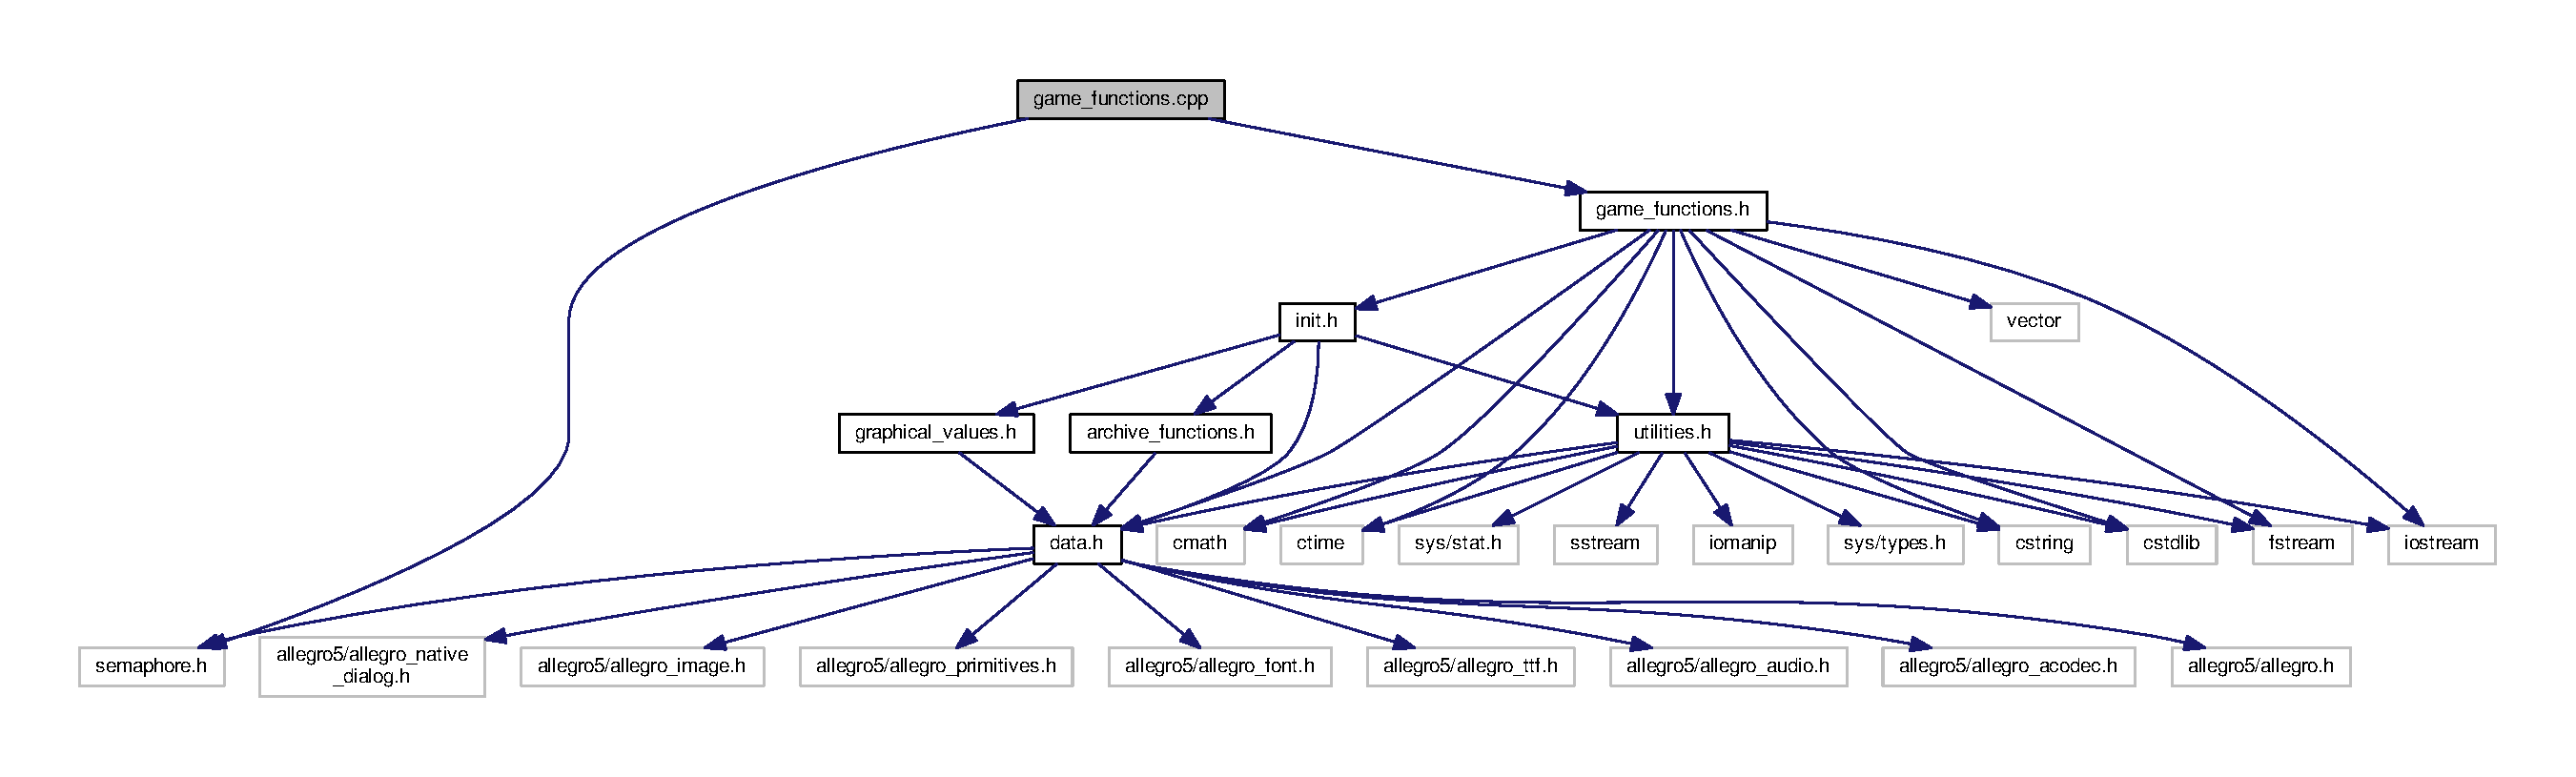
\includegraphics[width=350pt]{d8/d20/game__functions_8cpp__incl}
\end{center}
\end{figure}
\subsection*{Funzioni}
\begin{DoxyCompactItemize}
\item 
void $\ast$ \hyperlink{game__functions_8cpp_a4f01741d10ee6c94dcc93d71a3b39c04}{spawn\+\_\+asteroid\+\_\+thread} (void $\ast$mv)
\begin{DoxyCompactList}\small\item\em Funzione che implementa il consumer thread. \end{DoxyCompactList}\item 
void \hyperlink{game__functions_8cpp_a2a8678c0c49d26b7b3fc8dae6de25713}{sound\+\_\+play} (A\+L\+L\+E\+G\+R\+O\+\_\+\+S\+A\+M\+P\+LE $\ast$sound, const \hyperlink{data_8h_a56839c56ca6deb3cff5e21540ddb8218}{enable\+\_\+t} \&en\+\_\+sound)
\begin{DoxyCompactList}\small\item\em Funzione che fa partire il rispettivo suono del gioco, se i suoni sono attivati. \end{DoxyCompactList}\item 
void \hyperlink{game__functions_8cpp_a55bb6054017958a7940adc384b00b734}{music\+\_\+wa\+\_\+play} ()
\begin{DoxyCompactList}\small\item\em Funzione che fa partire la musica del gioco. \end{DoxyCompactList}\item 
\hyperlink{structasteroid__t}{asteroid\+\_\+t} \hyperlink{game__functions_8cpp_a9d3651675c457f8c8dbbf4b174c8e06a}{generate\+\_\+asteroid} (const \hyperlink{data_8h_a07b940e2e86eb4fc3f1e1e1843da0564}{asteroid\+\_\+special\+\_\+t} s, const int \&next\+\_\+p)
\begin{DoxyCompactList}\small\item\em Funzione che genera un singolo asteroide (di tipo compreso tra 3 e lev) in un punto casuale del bordo della zona di gioco. \end{DoxyCompactList}\item 
void \hyperlink{game__functions_8cpp_ae610b03423bc72bf50a76a18e5edce92}{move\+\_\+bullets} (\hyperlink{structbullet__t}{bullet\+\_\+t} $\ast$bullet, \hyperlink{structmatch__vars__t}{match\+\_\+vars\+\_\+t} \&match\+\_\+vars, \hyperlink{data_8h_a56839c56ca6deb3cff5e21540ddb8218}{enable\+\_\+t} \&en\+\_\+sound)
\begin{DoxyCompactList}\small\item\em Funzione che muove i bullets, e quando c\textquotesingle{}è una collisione viene definitivamente eliminato l\textquotesingle{}asteroide dalla lista, e aggiornati i bonus corrispondenti agli asteroidi distrutti. \end{DoxyCompactList}\item 
void \hyperlink{game__functions_8cpp_ab2d6354e392f2da433ab558560e82541}{move\+\_\+asteroids} (\hyperlink{data_8h_a452eef9acfcf76fb85e2c7ecf3b9ff90}{asteroid\+\_\+list} $\ast$ast\+\_\+queues, const int \&extract\+\_\+index)
\begin{DoxyCompactList}\small\item\em Funzione che muove l\textquotesingle{}asteroide in relazione al suo angolo con lo shooter, in modo che segua la retta che congiunge shooter -\/ asteroide. \end{DoxyCompactList}\item 
void \hyperlink{game__functions_8cpp_a378814aa4904070e808e0ac446a90295}{move\+\_\+shooter} (\hyperlink{structshooter__t}{shooter\+\_\+t} \&shooter, const \hyperlink{data_8h_a452eef9acfcf76fb85e2c7ecf3b9ff90}{asteroid\+\_\+list} $\ast$ast\+\_\+queues, const int current\+\_\+asteroid)
\begin{DoxyCompactList}\small\item\em Funzione che ruota lo shooter in base all\textquotesingle{}asteroide puntato. \end{DoxyCompactList}\item 
bool \hyperlink{game__functions_8cpp_a678c1013bf4f3a44b140829f7954e0f7}{check\+\_\+gameover} (\hyperlink{data_8h_a452eef9acfcf76fb85e2c7ecf3b9ff90}{asteroid\+\_\+list} $\ast$ast\+\_\+queues, const \hyperlink{structshooter__t}{shooter\+\_\+t} \&shooter, const \hyperlink{structbullet__t}{bullet\+\_\+t} $\ast$arr\+\_\+bullet)
\begin{DoxyCompactList}\small\item\em Funzione che, in base alla posizione degli asteroidi in gioco e dello shooter, controlla se ci siano collisioni, ovvero se lo shooter e un asteroide in gioco si siano toccati, e il gioco in questo caso finisce. \end{DoxyCompactList}\item 
float \hyperlink{game__functions_8cpp_a0afa627f8960d4dd4b67274fdf64fe0a}{check\+\_\+distance} (const \hyperlink{data_8h_a452eef9acfcf76fb85e2c7ecf3b9ff90}{asteroid\+\_\+list} $\ast$ast\+\_\+queues, const \hyperlink{structbullet__t}{bullet\+\_\+t} $\ast$arr\+\_\+bullet, const \hyperlink{structshooter__t}{shooter\+\_\+t} \&shooter)
\begin{DoxyCompactList}\small\item\em Funzione che restitusice la distanza tra il meteorite più vicino all\textquotesingle{}asteroide e l\textquotesingle{}asteroide stesso. \end{DoxyCompactList}\item 
void \hyperlink{game__functions_8cpp_a265dd35de6568690392ca63124fccccb}{check\+\_\+shield} (\hyperlink{structmatch__vars__t}{match\+\_\+vars\+\_\+t} \&match\+\_\+vars, \hyperlink{structbullet__t}{bullet\+\_\+t} $\ast$arr\+\_\+bullet, \hyperlink{structshooter__t}{shooter\+\_\+t} \&shooter, \hyperlink{data_8h_a56839c56ca6deb3cff5e21540ddb8218}{enable\+\_\+t} \&en\+\_\+sound)
\begin{DoxyCompactList}\small\item\em Funzione che controlla lo stato dello scudo. \end{DoxyCompactList}\item 
void \hyperlink{game__functions_8cpp_a21d0ec8c5d68d9d7016f4bf884d33e9a}{handler\+\_\+timer} (A\+L\+L\+E\+G\+R\+O\+\_\+\+E\+V\+E\+NT ev, \hyperlink{structmatch__vars__t}{match\+\_\+vars\+\_\+t} \&match\+\_\+vars, \hyperlink{structsettings__t}{settings\+\_\+t} \&settings)
\begin{DoxyCompactList}\small\item\em Funzione di routine che gestisce l\textquotesingle{}evento della scadenza di un timer. \end{DoxyCompactList}\item 
void \hyperlink{game__functions_8cpp_a8fa1c1282d2161623c1488dc68b085c7}{handler\+\_\+key\+\_\+pressed} (A\+L\+L\+E\+G\+R\+O\+\_\+\+E\+V\+E\+NT ev, \hyperlink{structmatch__vars__t}{match\+\_\+vars\+\_\+t} \&match\+\_\+vars, \hyperlink{structbullet__t}{bullet\+\_\+t} $\ast$arr\+\_\+bullet, \hyperlink{structshooter__t}{shooter\+\_\+t} \&shooter, \hyperlink{structsettings__t}{settings\+\_\+t} \&settings)
\begin{DoxyCompactList}\small\item\em Funzione di routine che gestisce l\textquotesingle{}evento della scadenza di un timer. \end{DoxyCompactList}\item 
void \hyperlink{game__functions_8cpp_a128182b533de18f8e11904ea47403c20}{change\+\_\+music} (const char $\ast$path, const \hyperlink{data_8h_a56839c56ca6deb3cff5e21540ddb8218}{enable\+\_\+t} \&music)
\begin{DoxyCompactList}\small\item\em Funzione che mette cambia la musica tra le varie schermate. \end{DoxyCompactList}\end{DoxyCompactItemize}


\subsection{Documentazione delle funzioni}
\mbox{\Hypertarget{game__functions_8cpp_a128182b533de18f8e11904ea47403c20}\label{game__functions_8cpp_a128182b533de18f8e11904ea47403c20}} 
\index{game\+\_\+functions.\+cpp@{game\+\_\+functions.\+cpp}!change\+\_\+music@{change\+\_\+music}}
\index{change\+\_\+music@{change\+\_\+music}!game\+\_\+functions.\+cpp@{game\+\_\+functions.\+cpp}}
\subsubsection{\texorpdfstring{change\+\_\+music()}{change\_music()}}
{\footnotesize\ttfamily void change\+\_\+music (\begin{DoxyParamCaption}\item[{const char $\ast$}]{path,  }\item[{const \hyperlink{data_8h_a56839c56ca6deb3cff5e21540ddb8218}{enable\+\_\+t} \&}]{music }\end{DoxyParamCaption})}



Funzione che mette cambia la musica tra le varie schermate. 

~\newline
Parametri\+: ~\newline
1) path -\/ Percorso del nuovo audio. \mbox{\Hypertarget{game__functions_8cpp_a0afa627f8960d4dd4b67274fdf64fe0a}\label{game__functions_8cpp_a0afa627f8960d4dd4b67274fdf64fe0a}} 
\index{game\+\_\+functions.\+cpp@{game\+\_\+functions.\+cpp}!check\+\_\+distance@{check\+\_\+distance}}
\index{check\+\_\+distance@{check\+\_\+distance}!game\+\_\+functions.\+cpp@{game\+\_\+functions.\+cpp}}
\subsubsection{\texorpdfstring{check\+\_\+distance()}{check\_distance()}}
{\footnotesize\ttfamily float check\+\_\+distance (\begin{DoxyParamCaption}\item[{const \hyperlink{data_8h_a452eef9acfcf76fb85e2c7ecf3b9ff90}{asteroid\+\_\+list} $\ast$}]{ast\+\_\+queues,  }\item[{const \hyperlink{structbullet__t}{bullet\+\_\+t} $\ast$}]{arr\+\_\+bullet,  }\item[{const \hyperlink{structshooter__t}{shooter\+\_\+t} \&}]{shooter }\end{DoxyParamCaption})}



Funzione che restitusice la distanza tra il meteorite più vicino all\textquotesingle{}asteroide e l\textquotesingle{}asteroide stesso. 

Parametri\+: ~\newline
1) ast\+\_\+queues -\/ Vettore di liste di asteroidi; ~\newline
2) arr\+\_\+bullet -\/ Vettore dei proiettili ~\newline
3) shooter -\/ Informazioni relative allo shooter. \mbox{\Hypertarget{game__functions_8cpp_a678c1013bf4f3a44b140829f7954e0f7}\label{game__functions_8cpp_a678c1013bf4f3a44b140829f7954e0f7}} 
\index{game\+\_\+functions.\+cpp@{game\+\_\+functions.\+cpp}!check\+\_\+gameover@{check\+\_\+gameover}}
\index{check\+\_\+gameover@{check\+\_\+gameover}!game\+\_\+functions.\+cpp@{game\+\_\+functions.\+cpp}}
\subsubsection{\texorpdfstring{check\+\_\+gameover()}{check\_gameover()}}
{\footnotesize\ttfamily bool check\+\_\+gameover (\begin{DoxyParamCaption}\item[{\hyperlink{data_8h_a452eef9acfcf76fb85e2c7ecf3b9ff90}{asteroid\+\_\+list} $\ast$}]{ast\+\_\+queues,  }\item[{const \hyperlink{structshooter__t}{shooter\+\_\+t} \&}]{shooter,  }\item[{const \hyperlink{structbullet__t}{bullet\+\_\+t} $\ast$}]{arr\+\_\+bullet }\end{DoxyParamCaption})}



Funzione che, in base alla posizione degli asteroidi in gioco e dello shooter, controlla se ci siano collisioni, ovvero se lo shooter e un asteroide in gioco si siano toccati, e il gioco in questo caso finisce. 

~\newline
Parametri\+: ~\newline
1) ast\+\_\+queues -\/ Vettore di liste di asteroidi; ~\newline
2) shooter -\/ Informazioni relative allo shooter; ~\newline
3) arr\+\_\+bullet -\/ Vettore dei proiettili. \mbox{\Hypertarget{game__functions_8cpp_a265dd35de6568690392ca63124fccccb}\label{game__functions_8cpp_a265dd35de6568690392ca63124fccccb}} 
\index{game\+\_\+functions.\+cpp@{game\+\_\+functions.\+cpp}!check\+\_\+shield@{check\+\_\+shield}}
\index{check\+\_\+shield@{check\+\_\+shield}!game\+\_\+functions.\+cpp@{game\+\_\+functions.\+cpp}}
\subsubsection{\texorpdfstring{check\+\_\+shield()}{check\_shield()}}
{\footnotesize\ttfamily void check\+\_\+shield (\begin{DoxyParamCaption}\item[{\hyperlink{structmatch__vars__t}{match\+\_\+vars\+\_\+t} \&}]{match\+\_\+vars,  }\item[{\hyperlink{structbullet__t}{bullet\+\_\+t} $\ast$}]{arr\+\_\+bullet,  }\item[{\hyperlink{structshooter__t}{shooter\+\_\+t} \&}]{shooter,  }\item[{\hyperlink{data_8h_a56839c56ca6deb3cff5e21540ddb8218}{enable\+\_\+t} \&}]{en\+\_\+sound }\end{DoxyParamCaption})}



Funzione che controlla lo stato dello scudo. 

Se c\textquotesingle{}è gameover ma lo scudo è attivo grazie al bonus \textquotesingle{}shield\textquotesingle{}, l\textquotesingle{}asteroide che colpisce lo scudo viene distrutto. ~\newline
Parametri\+: ~\newline
2) match\+\_\+vars -\/ Contenitore delle variabili di gioco; ~\newline
2) arr\+\_\+bullet -\/ Vettore dei proiettili; ~\newline
3) shooter -\/ Informazioni relative allo shooter. \mbox{\Hypertarget{game__functions_8cpp_a9d3651675c457f8c8dbbf4b174c8e06a}\label{game__functions_8cpp_a9d3651675c457f8c8dbbf4b174c8e06a}} 
\index{game\+\_\+functions.\+cpp@{game\+\_\+functions.\+cpp}!generate\+\_\+asteroid@{generate\+\_\+asteroid}}
\index{generate\+\_\+asteroid@{generate\+\_\+asteroid}!game\+\_\+functions.\+cpp@{game\+\_\+functions.\+cpp}}
\subsubsection{\texorpdfstring{generate\+\_\+asteroid()}{generate\_asteroid()}}
{\footnotesize\ttfamily \hyperlink{structasteroid__t}{asteroid\+\_\+t} generate\+\_\+asteroid (\begin{DoxyParamCaption}\item[{const \hyperlink{data_8h_a07b940e2e86eb4fc3f1e1e1843da0564}{asteroid\+\_\+special\+\_\+t}}]{s,  }\item[{const int \&}]{next\+\_\+p }\end{DoxyParamCaption})}



Funzione che genera un singolo asteroide (di tipo compreso tra 3 e lev) in un punto casuale del bordo della zona di gioco. 

~\newline
Parametri\+: ~\newline
1) lev -\/ Livello attuale; ~\newline
2) v -\/ lingua della parole dell\textquotesingle{}asteroide ~\newline
3) s -\/ Caratteristiche speciali dell\textquotesingle{}asteroide ~\newline
4) next\+\_\+p -\/ In caso di conflitto, viene utilizzata come posizione in cui inserire l\textquotesingle{}asteroide \mbox{\Hypertarget{game__functions_8cpp_a8fa1c1282d2161623c1488dc68b085c7}\label{game__functions_8cpp_a8fa1c1282d2161623c1488dc68b085c7}} 
\index{game\+\_\+functions.\+cpp@{game\+\_\+functions.\+cpp}!handler\+\_\+key\+\_\+pressed@{handler\+\_\+key\+\_\+pressed}}
\index{handler\+\_\+key\+\_\+pressed@{handler\+\_\+key\+\_\+pressed}!game\+\_\+functions.\+cpp@{game\+\_\+functions.\+cpp}}
\subsubsection{\texorpdfstring{handler\+\_\+key\+\_\+pressed()}{handler\_key\_pressed()}}
{\footnotesize\ttfamily void handler\+\_\+key\+\_\+pressed (\begin{DoxyParamCaption}\item[{A\+L\+L\+E\+G\+R\+O\+\_\+\+E\+V\+E\+NT}]{ev,  }\item[{\hyperlink{structmatch__vars__t}{match\+\_\+vars\+\_\+t} \&}]{match\+\_\+vars,  }\item[{\hyperlink{structbullet__t}{bullet\+\_\+t} $\ast$}]{arr\+\_\+bullet,  }\item[{\hyperlink{structshooter__t}{shooter\+\_\+t} \&}]{shooter,  }\item[{\hyperlink{structsettings__t}{settings\+\_\+t} \&}]{settings }\end{DoxyParamCaption})}



Funzione di routine che gestisce l\textquotesingle{}evento della scadenza di un timer. 

In base al timer scaduto (spawn, shield, rallenty) genera l\textquotesingle{}evento associato. ~\newline
Parametri\+: ~\newline
1) ev -\/ Evento generato; ~\newline
2) match\+\_\+vars -\/ Contenitore delle variabili di gioco; ~\newline
3) arr\+\_\+bullet -\/ Vettore dei proiettili; ~\newline
4) shooter -\/ Informazioni relative allo shooter; ~\newline
5) settings -\/ Impostazioni di gioco. \mbox{\Hypertarget{game__functions_8cpp_a21d0ec8c5d68d9d7016f4bf884d33e9a}\label{game__functions_8cpp_a21d0ec8c5d68d9d7016f4bf884d33e9a}} 
\index{game\+\_\+functions.\+cpp@{game\+\_\+functions.\+cpp}!handler\+\_\+timer@{handler\+\_\+timer}}
\index{handler\+\_\+timer@{handler\+\_\+timer}!game\+\_\+functions.\+cpp@{game\+\_\+functions.\+cpp}}
\subsubsection{\texorpdfstring{handler\+\_\+timer()}{handler\_timer()}}
{\footnotesize\ttfamily void handler\+\_\+timer (\begin{DoxyParamCaption}\item[{A\+L\+L\+E\+G\+R\+O\+\_\+\+E\+V\+E\+NT}]{ev,  }\item[{\hyperlink{structmatch__vars__t}{match\+\_\+vars\+\_\+t} \&}]{match\+\_\+vars,  }\item[{\hyperlink{structsettings__t}{settings\+\_\+t} \&}]{settings }\end{DoxyParamCaption})}



Funzione di routine che gestisce l\textquotesingle{}evento della scadenza di un timer. 

In base al timer scaduto (spawn, shield, rallenty) genera l\textquotesingle{}evento associato. ~\newline
Parametri\+: ~\newline
1) ev -\/ Evento generato; ~\newline
2) match\+\_\+vars -\/ Contenitore dei tre timer; ~\newline
3) settings -\/ Impostazioni di gioco. \mbox{\Hypertarget{game__functions_8cpp_ab2d6354e392f2da433ab558560e82541}\label{game__functions_8cpp_ab2d6354e392f2da433ab558560e82541}} 
\index{game\+\_\+functions.\+cpp@{game\+\_\+functions.\+cpp}!move\+\_\+asteroids@{move\+\_\+asteroids}}
\index{move\+\_\+asteroids@{move\+\_\+asteroids}!game\+\_\+functions.\+cpp@{game\+\_\+functions.\+cpp}}
\subsubsection{\texorpdfstring{move\+\_\+asteroids()}{move\_asteroids()}}
{\footnotesize\ttfamily void move\+\_\+asteroids (\begin{DoxyParamCaption}\item[{\hyperlink{data_8h_a452eef9acfcf76fb85e2c7ecf3b9ff90}{asteroid\+\_\+list} $\ast$}]{ast\+\_\+queues,  }\item[{const int \&}]{extract\+\_\+index }\end{DoxyParamCaption})}



Funzione che muove l\textquotesingle{}asteroide in relazione al suo angolo con lo shooter, in modo che segua la retta che congiunge shooter -\/ asteroide. 

~\newline
Parametri\+: ~\newline
1) ast\+\_\+queues -\/ Vettore di liste di asteroidi; ~\newline
2) extract\+\_\+index -\/ Indice dell\textquotesingle{}asteroide in campo ma da non far comparire. \mbox{\Hypertarget{game__functions_8cpp_ae610b03423bc72bf50a76a18e5edce92}\label{game__functions_8cpp_ae610b03423bc72bf50a76a18e5edce92}} 
\index{game\+\_\+functions.\+cpp@{game\+\_\+functions.\+cpp}!move\+\_\+bullets@{move\+\_\+bullets}}
\index{move\+\_\+bullets@{move\+\_\+bullets}!game\+\_\+functions.\+cpp@{game\+\_\+functions.\+cpp}}
\subsubsection{\texorpdfstring{move\+\_\+bullets()}{move\_bullets()}}
{\footnotesize\ttfamily void move\+\_\+bullets (\begin{DoxyParamCaption}\item[{\hyperlink{structbullet__t}{bullet\+\_\+t} $\ast$}]{bullet,  }\item[{\hyperlink{structmatch__vars__t}{match\+\_\+vars\+\_\+t} \&}]{match\+\_\+vars,  }\item[{\hyperlink{data_8h_a56839c56ca6deb3cff5e21540ddb8218}{enable\+\_\+t} \&}]{en\+\_\+sound }\end{DoxyParamCaption})}



Funzione che muove i bullets, e quando c\textquotesingle{}è una collisione viene definitivamente eliminato l\textquotesingle{}asteroide dalla lista, e aggiornati i bonus corrispondenti agli asteroidi distrutti. 

~\newline
Parametri\+: ~\newline
1) bullet -\/ Vettore dei bullet; ~\newline
2) match\+\_\+vars -\/ Contenitore delle variabili di gioco; ~\newline
3) items -\/ Vettore dei bonus. \mbox{\Hypertarget{game__functions_8cpp_a378814aa4904070e808e0ac446a90295}\label{game__functions_8cpp_a378814aa4904070e808e0ac446a90295}} 
\index{game\+\_\+functions.\+cpp@{game\+\_\+functions.\+cpp}!move\+\_\+shooter@{move\+\_\+shooter}}
\index{move\+\_\+shooter@{move\+\_\+shooter}!game\+\_\+functions.\+cpp@{game\+\_\+functions.\+cpp}}
\subsubsection{\texorpdfstring{move\+\_\+shooter()}{move\_shooter()}}
{\footnotesize\ttfamily void move\+\_\+shooter (\begin{DoxyParamCaption}\item[{\hyperlink{structshooter__t}{shooter\+\_\+t} \&}]{shooter,  }\item[{const \hyperlink{data_8h_a452eef9acfcf76fb85e2c7ecf3b9ff90}{asteroid\+\_\+list} $\ast$}]{ast\+\_\+queues,  }\item[{const int}]{current\+\_\+asteroid }\end{DoxyParamCaption})}



Funzione che ruota lo shooter in base all\textquotesingle{}asteroide puntato. 

~\newline
Parametri\+: ~\newline
1) shooter -\/ Informazioni relative allo shooter; ~\newline
2) ast\+\_\+queues -\/ Vettore di liste di asteroidi; ~\newline
3) current\+\_\+asteroid -\/ Carattere corrispondente all\textquotesingle{}asteroide puntato. \mbox{\Hypertarget{game__functions_8cpp_a55bb6054017958a7940adc384b00b734}\label{game__functions_8cpp_a55bb6054017958a7940adc384b00b734}} 
\index{game\+\_\+functions.\+cpp@{game\+\_\+functions.\+cpp}!music\+\_\+wa\+\_\+play@{music\+\_\+wa\+\_\+play}}
\index{music\+\_\+wa\+\_\+play@{music\+\_\+wa\+\_\+play}!game\+\_\+functions.\+cpp@{game\+\_\+functions.\+cpp}}
\subsubsection{\texorpdfstring{music\+\_\+wa\+\_\+play()}{music\_wa\_play()}}
{\footnotesize\ttfamily void music\+\_\+wa\+\_\+play (\begin{DoxyParamCaption}{ }\end{DoxyParamCaption})}



Funzione che fa partire la musica del gioco. 

\mbox{\Hypertarget{game__functions_8cpp_a2a8678c0c49d26b7b3fc8dae6de25713}\label{game__functions_8cpp_a2a8678c0c49d26b7b3fc8dae6de25713}} 
\index{game\+\_\+functions.\+cpp@{game\+\_\+functions.\+cpp}!sound\+\_\+play@{sound\+\_\+play}}
\index{sound\+\_\+play@{sound\+\_\+play}!game\+\_\+functions.\+cpp@{game\+\_\+functions.\+cpp}}
\subsubsection{\texorpdfstring{sound\+\_\+play()}{sound\_play()}}
{\footnotesize\ttfamily void sound\+\_\+play (\begin{DoxyParamCaption}\item[{A\+L\+L\+E\+G\+R\+O\+\_\+\+S\+A\+M\+P\+LE $\ast$}]{sound,  }\item[{const \hyperlink{data_8h_a56839c56ca6deb3cff5e21540ddb8218}{enable\+\_\+t} \&}]{en\+\_\+sound }\end{DoxyParamCaption})}



Funzione che fa partire il rispettivo suono del gioco, se i suoni sono attivati. 

Parametri\+: ~\newline
1) sound -\/ Suono da far partire; ~\newline
2) en\+\_\+sound -\/ Impostazioni che indica se i suoni sono O\+N/\+O\+FF. \mbox{\Hypertarget{game__functions_8cpp_a4f01741d10ee6c94dcc93d71a3b39c04}\label{game__functions_8cpp_a4f01741d10ee6c94dcc93d71a3b39c04}} 
\index{game\+\_\+functions.\+cpp@{game\+\_\+functions.\+cpp}!spawn\+\_\+asteroid\+\_\+thread@{spawn\+\_\+asteroid\+\_\+thread}}
\index{spawn\+\_\+asteroid\+\_\+thread@{spawn\+\_\+asteroid\+\_\+thread}!game\+\_\+functions.\+cpp@{game\+\_\+functions.\+cpp}}
\subsubsection{\texorpdfstring{spawn\+\_\+asteroid\+\_\+thread()}{spawn\_asteroid\_thread()}}
{\footnotesize\ttfamily void$\ast$ spawn\+\_\+asteroid\+\_\+thread (\begin{DoxyParamCaption}\item[{void $\ast$}]{mv }\end{DoxyParamCaption})}



Funzione che implementa il consumer thread. 

Ad intervalli regolari viene estratta una parola ed inserita all\textquotesingle{}interno del gioco. ~\newline
Parametri\+: ~\newline
1) mv -\/ Puntatore alle match vars, le variabili di gioco; ~\newline

\hypertarget{game__functions_8h}{}\section{Riferimenti per il file game\+\_\+functions.\+h}
\label{game__functions_8h}\index{game\+\_\+functions.\+h@{game\+\_\+functions.\+h}}
{\ttfamily \#include \char`\"{}data.\+h\char`\"{}}\newline
{\ttfamily \#include \char`\"{}utilities.\+h\char`\"{}}\newline
{\ttfamily \#include \char`\"{}init.\+h\char`\"{}}\newline
{\ttfamily \#include $<$iostream$>$}\newline
{\ttfamily \#include $<$vector$>$}\newline
{\ttfamily \#include $<$fstream$>$}\newline
{\ttfamily \#include $<$cmath$>$}\newline
{\ttfamily \#include $<$ctime$>$}\newline
{\ttfamily \#include $<$cstring$>$}\newline
{\ttfamily \#include $<$cstdlib$>$}\newline
Grafo delle dipendenze di inclusione per game\+\_\+functions.\+h\+:\nopagebreak
\begin{figure}[H]
\begin{center}
\leavevmode
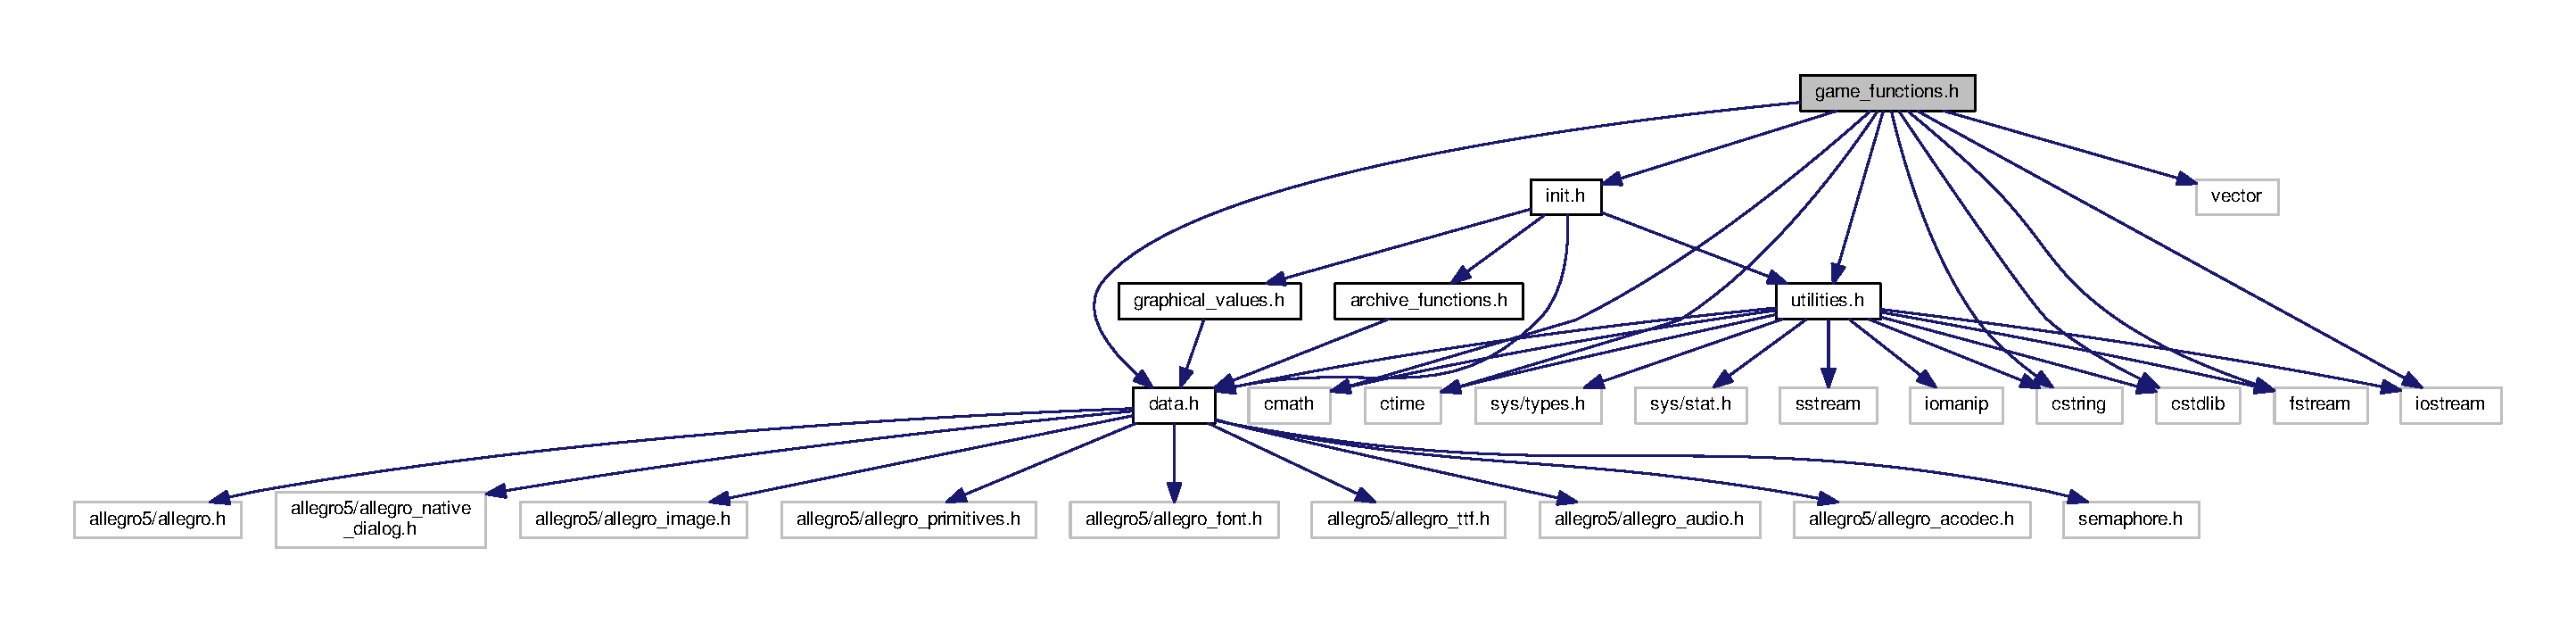
\includegraphics[width=350pt]{d7/dd4/game__functions_8h__incl}
\end{center}
\end{figure}
Questo grafo mostra quali altri file includono direttamente o indirettamente questo file\+:\nopagebreak
\begin{figure}[H]
\begin{center}
\leavevmode
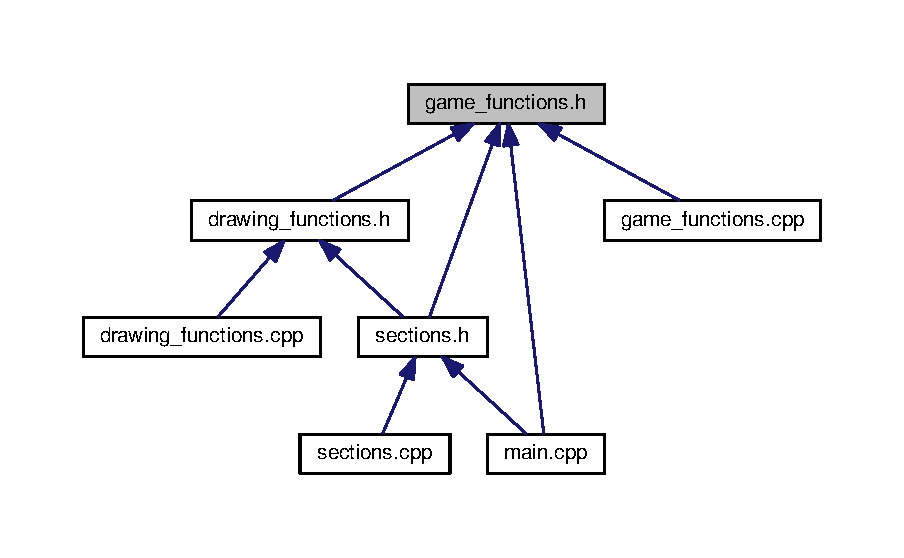
\includegraphics[width=350pt]{d2/dd8/game__functions_8h__dep__incl}
\end{center}
\end{figure}
\subsection*{Funzioni}
\begin{DoxyCompactItemize}
\item 
void \hyperlink{game__functions_8h_a2a8678c0c49d26b7b3fc8dae6de25713}{sound\+\_\+play} (A\+L\+L\+E\+G\+R\+O\+\_\+\+S\+A\+M\+P\+LE $\ast$sound, const \hyperlink{data_8h_a56839c56ca6deb3cff5e21540ddb8218}{enable\+\_\+t} \&en\+\_\+sound)
\begin{DoxyCompactList}\small\item\em Funzione che fa partire il rispettivo suono del gioco, se i suoni sono attivati. \end{DoxyCompactList}\item 
void \hyperlink{game__functions_8h_a55bb6054017958a7940adc384b00b734}{music\+\_\+wa\+\_\+play} ()
\begin{DoxyCompactList}\small\item\em Funzione che fa partire la musica del gioco. \end{DoxyCompactList}\item 
\hyperlink{structasteroid__t}{asteroid\+\_\+t} \hyperlink{game__functions_8h_a9d3651675c457f8c8dbbf4b174c8e06a}{generate\+\_\+asteroid} (const \hyperlink{data_8h_a07b940e2e86eb4fc3f1e1e1843da0564}{asteroid\+\_\+special\+\_\+t} s, const int \&next\+\_\+p)
\begin{DoxyCompactList}\small\item\em Funzione che genera un singolo asteroide (di tipo compreso tra 3 e lev) in un punto casuale del bordo della zona di gioco. \end{DoxyCompactList}\item 
void \hyperlink{game__functions_8h_ae610b03423bc72bf50a76a18e5edce92}{move\+\_\+bullets} (\hyperlink{structbullet__t}{bullet\+\_\+t} $\ast$bullet, \hyperlink{structmatch__vars__t}{match\+\_\+vars\+\_\+t} \&match\+\_\+vars, \hyperlink{data_8h_a56839c56ca6deb3cff5e21540ddb8218}{enable\+\_\+t} \&en\+\_\+sound)
\begin{DoxyCompactList}\small\item\em Funzione che muove i bullets, e quando c\textquotesingle{}è una collisione viene definitivamente eliminato l\textquotesingle{}asteroide dalla lista, e aggiornati i bonus corrispondenti agli asteroidi distrutti. \end{DoxyCompactList}\item 
void \hyperlink{game__functions_8h_ab2d6354e392f2da433ab558560e82541}{move\+\_\+asteroids} (\hyperlink{data_8h_a452eef9acfcf76fb85e2c7ecf3b9ff90}{asteroid\+\_\+list} $\ast$ast\+\_\+queues, const int \&extract\+\_\+index)
\begin{DoxyCompactList}\small\item\em Funzione che muove l\textquotesingle{}asteroide in relazione al suo angolo con lo shooter, in modo che segua la retta che congiunge shooter -\/ asteroide. \end{DoxyCompactList}\item 
void \hyperlink{game__functions_8h_a378814aa4904070e808e0ac446a90295}{move\+\_\+shooter} (\hyperlink{structshooter__t}{shooter\+\_\+t} \&shooter, const \hyperlink{data_8h_a452eef9acfcf76fb85e2c7ecf3b9ff90}{asteroid\+\_\+list} $\ast$ast\+\_\+queues, const int current\+\_\+asteroid)
\begin{DoxyCompactList}\small\item\em Funzione che ruota lo shooter in base all\textquotesingle{}asteroide puntato. \end{DoxyCompactList}\item 
bool \hyperlink{game__functions_8h_a678c1013bf4f3a44b140829f7954e0f7}{check\+\_\+gameover} (\hyperlink{data_8h_a452eef9acfcf76fb85e2c7ecf3b9ff90}{asteroid\+\_\+list} $\ast$ast\+\_\+queues, const \hyperlink{structshooter__t}{shooter\+\_\+t} \&shooter, const \hyperlink{structbullet__t}{bullet\+\_\+t} $\ast$arr\+\_\+bullet)
\begin{DoxyCompactList}\small\item\em Funzione che, in base alla posizione degli asteroidi in gioco e dello shooter, controlla se ci siano collisioni, ovvero se lo shooter e un asteroide in gioco si siano toccati, e il gioco in questo caso finisce. \end{DoxyCompactList}\item 
float \hyperlink{game__functions_8h_a0afa627f8960d4dd4b67274fdf64fe0a}{check\+\_\+distance} (const \hyperlink{data_8h_a452eef9acfcf76fb85e2c7ecf3b9ff90}{asteroid\+\_\+list} $\ast$ast\+\_\+queues, const \hyperlink{structbullet__t}{bullet\+\_\+t} $\ast$arr\+\_\+bullet, const \hyperlink{structshooter__t}{shooter\+\_\+t} \&shooter)
\begin{DoxyCompactList}\small\item\em Funzione che restitusice la distanza tra il meteorite più vicino all\textquotesingle{}asteroide e l\textquotesingle{}asteroide stesso. \end{DoxyCompactList}\item 
void \hyperlink{game__functions_8h_a265dd35de6568690392ca63124fccccb}{check\+\_\+shield} (\hyperlink{structmatch__vars__t}{match\+\_\+vars\+\_\+t} \&match\+\_\+vars, \hyperlink{structbullet__t}{bullet\+\_\+t} $\ast$arr\+\_\+bullet, \hyperlink{structshooter__t}{shooter\+\_\+t} \&shooter, \hyperlink{data_8h_a56839c56ca6deb3cff5e21540ddb8218}{enable\+\_\+t} \&en\+\_\+sound)
\begin{DoxyCompactList}\small\item\em Funzione che controlla lo stato dello scudo. \end{DoxyCompactList}\item 
void \hyperlink{game__functions_8h_a21d0ec8c5d68d9d7016f4bf884d33e9a}{handler\+\_\+timer} (A\+L\+L\+E\+G\+R\+O\+\_\+\+E\+V\+E\+NT ev, \hyperlink{structmatch__vars__t}{match\+\_\+vars\+\_\+t} \&match\+\_\+vars, \hyperlink{structsettings__t}{settings\+\_\+t} \&settings)
\begin{DoxyCompactList}\small\item\em Funzione di routine che gestisce l\textquotesingle{}evento della scadenza di un timer. \end{DoxyCompactList}\item 
void \hyperlink{game__functions_8h_a8fa1c1282d2161623c1488dc68b085c7}{handler\+\_\+key\+\_\+pressed} (A\+L\+L\+E\+G\+R\+O\+\_\+\+E\+V\+E\+NT ev, \hyperlink{structmatch__vars__t}{match\+\_\+vars\+\_\+t} \&match\+\_\+vars, \hyperlink{structbullet__t}{bullet\+\_\+t} $\ast$arr\+\_\+bullet, \hyperlink{structshooter__t}{shooter\+\_\+t} \&shooter, \hyperlink{structsettings__t}{settings\+\_\+t} \&settings)
\begin{DoxyCompactList}\small\item\em Funzione di routine che gestisce l\textquotesingle{}evento della scadenza di un timer. \end{DoxyCompactList}\item 
void \hyperlink{game__functions_8h_a128182b533de18f8e11904ea47403c20}{change\+\_\+music} (const char $\ast$path, const \hyperlink{data_8h_a56839c56ca6deb3cff5e21540ddb8218}{enable\+\_\+t} \&music)
\begin{DoxyCompactList}\small\item\em Funzione che mette cambia la musica tra le varie schermate. \end{DoxyCompactList}\item 
void $\ast$ \hyperlink{game__functions_8h_a4f01741d10ee6c94dcc93d71a3b39c04}{spawn\+\_\+asteroid\+\_\+thread} (void $\ast$mv)
\begin{DoxyCompactList}\small\item\em Funzione che implementa il consumer thread. \end{DoxyCompactList}\end{DoxyCompactItemize}
\subsection*{Variabili}
\begin{DoxyCompactItemize}
\item 
\hyperlink{structdisplay__info__t}{display\+\_\+info\+\_\+t} \hyperlink{game__functions_8h_a781a8df874545e4f5bff5f8a446d1963}{display\+\_\+info}
\item 
A\+L\+L\+E\+G\+R\+O\+\_\+\+S\+A\+M\+P\+LE $\ast$ \hyperlink{game__functions_8h_aaf63227dc3c1f6203248971c305a3e11}{music\+\_\+wa}
\item 
\hyperlink{structplaywa__gv__t}{playwa\+\_\+gv\+\_\+t} \hyperlink{game__functions_8h_a38bfadb0325688402bf1999301ca2a1b}{P\+L\+A\+Y\+W\+A\+\_\+\+GV}
\begin{DoxyCompactList}\small\item\em Struct contenente le proporzioni grafiche della schermata di gioco. \end{DoxyCompactList}\item 
\hyperlink{structthread__manager__t}{thread\+\_\+manager\+\_\+t} \hyperlink{game__functions_8h_ad04f177b84df22adea5536cbae88451b}{thread\+\_\+manager}
\item 
\hyperlink{structwords__buffer__t}{words\+\_\+buffer\+\_\+t} \hyperlink{game__functions_8h_aaa25f9883d8c134861353b1bf5e00846}{words\+\_\+buffer}
\end{DoxyCompactItemize}


\subsection{Documentazione delle funzioni}
\mbox{\Hypertarget{game__functions_8h_a128182b533de18f8e11904ea47403c20}\label{game__functions_8h_a128182b533de18f8e11904ea47403c20}} 
\index{game\+\_\+functions.\+h@{game\+\_\+functions.\+h}!change\+\_\+music@{change\+\_\+music}}
\index{change\+\_\+music@{change\+\_\+music}!game\+\_\+functions.\+h@{game\+\_\+functions.\+h}}
\subsubsection{\texorpdfstring{change\+\_\+music()}{change\_music()}}
{\footnotesize\ttfamily void change\+\_\+music (\begin{DoxyParamCaption}\item[{const char $\ast$}]{path,  }\item[{const \hyperlink{data_8h_a56839c56ca6deb3cff5e21540ddb8218}{enable\+\_\+t} \&}]{music }\end{DoxyParamCaption})}



Funzione che mette cambia la musica tra le varie schermate. 

~\newline
Parametri\+: ~\newline
1) path -\/ Percorso del nuovo audio. \mbox{\Hypertarget{game__functions_8h_a0afa627f8960d4dd4b67274fdf64fe0a}\label{game__functions_8h_a0afa627f8960d4dd4b67274fdf64fe0a}} 
\index{game\+\_\+functions.\+h@{game\+\_\+functions.\+h}!check\+\_\+distance@{check\+\_\+distance}}
\index{check\+\_\+distance@{check\+\_\+distance}!game\+\_\+functions.\+h@{game\+\_\+functions.\+h}}
\subsubsection{\texorpdfstring{check\+\_\+distance()}{check\_distance()}}
{\footnotesize\ttfamily float check\+\_\+distance (\begin{DoxyParamCaption}\item[{const \hyperlink{data_8h_a452eef9acfcf76fb85e2c7ecf3b9ff90}{asteroid\+\_\+list} $\ast$}]{ast\+\_\+queues,  }\item[{const \hyperlink{structbullet__t}{bullet\+\_\+t} $\ast$}]{arr\+\_\+bullet,  }\item[{const \hyperlink{structshooter__t}{shooter\+\_\+t} \&}]{shooter }\end{DoxyParamCaption})}



Funzione che restitusice la distanza tra il meteorite più vicino all\textquotesingle{}asteroide e l\textquotesingle{}asteroide stesso. 

Parametri\+: ~\newline
1) ast\+\_\+queues -\/ Vettore di liste di asteroidi; ~\newline
2) arr\+\_\+bullet -\/ Vettore dei proiettili ~\newline
3) shooter -\/ Informazioni relative allo shooter. \mbox{\Hypertarget{game__functions_8h_a678c1013bf4f3a44b140829f7954e0f7}\label{game__functions_8h_a678c1013bf4f3a44b140829f7954e0f7}} 
\index{game\+\_\+functions.\+h@{game\+\_\+functions.\+h}!check\+\_\+gameover@{check\+\_\+gameover}}
\index{check\+\_\+gameover@{check\+\_\+gameover}!game\+\_\+functions.\+h@{game\+\_\+functions.\+h}}
\subsubsection{\texorpdfstring{check\+\_\+gameover()}{check\_gameover()}}
{\footnotesize\ttfamily bool check\+\_\+gameover (\begin{DoxyParamCaption}\item[{\hyperlink{data_8h_a452eef9acfcf76fb85e2c7ecf3b9ff90}{asteroid\+\_\+list} $\ast$}]{ast\+\_\+queues,  }\item[{const \hyperlink{structshooter__t}{shooter\+\_\+t} \&}]{shooter,  }\item[{const \hyperlink{structbullet__t}{bullet\+\_\+t} $\ast$}]{arr\+\_\+bullet }\end{DoxyParamCaption})}



Funzione che, in base alla posizione degli asteroidi in gioco e dello shooter, controlla se ci siano collisioni, ovvero se lo shooter e un asteroide in gioco si siano toccati, e il gioco in questo caso finisce. 

~\newline
Parametri\+: ~\newline
1) ast\+\_\+queues -\/ Vettore di liste di asteroidi; ~\newline
2) shooter -\/ Informazioni relative allo shooter; ~\newline
3) arr\+\_\+bullet -\/ Vettore dei proiettili. \mbox{\Hypertarget{game__functions_8h_a265dd35de6568690392ca63124fccccb}\label{game__functions_8h_a265dd35de6568690392ca63124fccccb}} 
\index{game\+\_\+functions.\+h@{game\+\_\+functions.\+h}!check\+\_\+shield@{check\+\_\+shield}}
\index{check\+\_\+shield@{check\+\_\+shield}!game\+\_\+functions.\+h@{game\+\_\+functions.\+h}}
\subsubsection{\texorpdfstring{check\+\_\+shield()}{check\_shield()}}
{\footnotesize\ttfamily void check\+\_\+shield (\begin{DoxyParamCaption}\item[{\hyperlink{structmatch__vars__t}{match\+\_\+vars\+\_\+t} \&}]{match\+\_\+vars,  }\item[{\hyperlink{structbullet__t}{bullet\+\_\+t} $\ast$}]{arr\+\_\+bullet,  }\item[{\hyperlink{structshooter__t}{shooter\+\_\+t} \&}]{shooter,  }\item[{\hyperlink{data_8h_a56839c56ca6deb3cff5e21540ddb8218}{enable\+\_\+t} \&}]{en\+\_\+sound }\end{DoxyParamCaption})}



Funzione che controlla lo stato dello scudo. 

Se c\textquotesingle{}è gameover ma lo scudo è attivo grazie al bonus \textquotesingle{}shield\textquotesingle{}, l\textquotesingle{}asteroide che colpisce lo scudo viene distrutto. ~\newline
Parametri\+: ~\newline
2) match\+\_\+vars -\/ Contenitore delle variabili di gioco; ~\newline
2) arr\+\_\+bullet -\/ Vettore dei proiettili; ~\newline
3) shooter -\/ Informazioni relative allo shooter. \mbox{\Hypertarget{game__functions_8h_a9d3651675c457f8c8dbbf4b174c8e06a}\label{game__functions_8h_a9d3651675c457f8c8dbbf4b174c8e06a}} 
\index{game\+\_\+functions.\+h@{game\+\_\+functions.\+h}!generate\+\_\+asteroid@{generate\+\_\+asteroid}}
\index{generate\+\_\+asteroid@{generate\+\_\+asteroid}!game\+\_\+functions.\+h@{game\+\_\+functions.\+h}}
\subsubsection{\texorpdfstring{generate\+\_\+asteroid()}{generate\_asteroid()}}
{\footnotesize\ttfamily \hyperlink{structasteroid__t}{asteroid\+\_\+t} generate\+\_\+asteroid (\begin{DoxyParamCaption}\item[{const \hyperlink{data_8h_a07b940e2e86eb4fc3f1e1e1843da0564}{asteroid\+\_\+special\+\_\+t}}]{s,  }\item[{const int \&}]{next\+\_\+p }\end{DoxyParamCaption})}



Funzione che genera un singolo asteroide (di tipo compreso tra 3 e lev) in un punto casuale del bordo della zona di gioco. 

~\newline
Parametri\+: ~\newline
1) lev -\/ Livello attuale; ~\newline
2) v -\/ lingua della parole dell\textquotesingle{}asteroide ~\newline
3) s -\/ Caratteristiche speciali dell\textquotesingle{}asteroide ~\newline
4) next\+\_\+p -\/ In caso di conflitto, viene utilizzata come posizione in cui inserire l\textquotesingle{}asteroide \mbox{\Hypertarget{game__functions_8h_a8fa1c1282d2161623c1488dc68b085c7}\label{game__functions_8h_a8fa1c1282d2161623c1488dc68b085c7}} 
\index{game\+\_\+functions.\+h@{game\+\_\+functions.\+h}!handler\+\_\+key\+\_\+pressed@{handler\+\_\+key\+\_\+pressed}}
\index{handler\+\_\+key\+\_\+pressed@{handler\+\_\+key\+\_\+pressed}!game\+\_\+functions.\+h@{game\+\_\+functions.\+h}}
\subsubsection{\texorpdfstring{handler\+\_\+key\+\_\+pressed()}{handler\_key\_pressed()}}
{\footnotesize\ttfamily void handler\+\_\+key\+\_\+pressed (\begin{DoxyParamCaption}\item[{A\+L\+L\+E\+G\+R\+O\+\_\+\+E\+V\+E\+NT}]{ev,  }\item[{\hyperlink{structmatch__vars__t}{match\+\_\+vars\+\_\+t} \&}]{match\+\_\+vars,  }\item[{\hyperlink{structbullet__t}{bullet\+\_\+t} $\ast$}]{arr\+\_\+bullet,  }\item[{\hyperlink{structshooter__t}{shooter\+\_\+t} \&}]{shooter,  }\item[{\hyperlink{structsettings__t}{settings\+\_\+t} \&}]{settings }\end{DoxyParamCaption})}



Funzione di routine che gestisce l\textquotesingle{}evento della scadenza di un timer. 

In base al timer scaduto (spawn, shield, rallenty) genera l\textquotesingle{}evento associato. ~\newline
Parametri\+: ~\newline
1) ev -\/ Evento generato; ~\newline
2) match\+\_\+vars -\/ Contenitore delle variabili di gioco; ~\newline
3) arr\+\_\+bullet -\/ Vettore dei proiettili; ~\newline
4) shooter -\/ Informazioni relative allo shooter; ~\newline
5) settings -\/ Impostazioni di gioco. \mbox{\Hypertarget{game__functions_8h_a21d0ec8c5d68d9d7016f4bf884d33e9a}\label{game__functions_8h_a21d0ec8c5d68d9d7016f4bf884d33e9a}} 
\index{game\+\_\+functions.\+h@{game\+\_\+functions.\+h}!handler\+\_\+timer@{handler\+\_\+timer}}
\index{handler\+\_\+timer@{handler\+\_\+timer}!game\+\_\+functions.\+h@{game\+\_\+functions.\+h}}
\subsubsection{\texorpdfstring{handler\+\_\+timer()}{handler\_timer()}}
{\footnotesize\ttfamily void handler\+\_\+timer (\begin{DoxyParamCaption}\item[{A\+L\+L\+E\+G\+R\+O\+\_\+\+E\+V\+E\+NT}]{ev,  }\item[{\hyperlink{structmatch__vars__t}{match\+\_\+vars\+\_\+t} \&}]{match\+\_\+vars,  }\item[{\hyperlink{structsettings__t}{settings\+\_\+t} \&}]{settings }\end{DoxyParamCaption})}



Funzione di routine che gestisce l\textquotesingle{}evento della scadenza di un timer. 

In base al timer scaduto (spawn, shield, rallenty) genera l\textquotesingle{}evento associato. ~\newline
Parametri\+: ~\newline
1) ev -\/ Evento generato; ~\newline
2) match\+\_\+vars -\/ Contenitore dei tre timer; ~\newline
3) settings -\/ Impostazioni di gioco. \mbox{\Hypertarget{game__functions_8h_ab2d6354e392f2da433ab558560e82541}\label{game__functions_8h_ab2d6354e392f2da433ab558560e82541}} 
\index{game\+\_\+functions.\+h@{game\+\_\+functions.\+h}!move\+\_\+asteroids@{move\+\_\+asteroids}}
\index{move\+\_\+asteroids@{move\+\_\+asteroids}!game\+\_\+functions.\+h@{game\+\_\+functions.\+h}}
\subsubsection{\texorpdfstring{move\+\_\+asteroids()}{move\_asteroids()}}
{\footnotesize\ttfamily void move\+\_\+asteroids (\begin{DoxyParamCaption}\item[{\hyperlink{data_8h_a452eef9acfcf76fb85e2c7ecf3b9ff90}{asteroid\+\_\+list} $\ast$}]{ast\+\_\+queues,  }\item[{const int \&}]{extract\+\_\+index }\end{DoxyParamCaption})}



Funzione che muove l\textquotesingle{}asteroide in relazione al suo angolo con lo shooter, in modo che segua la retta che congiunge shooter -\/ asteroide. 

~\newline
Parametri\+: ~\newline
1) ast\+\_\+queues -\/ Vettore di liste di asteroidi; ~\newline
2) extract\+\_\+index -\/ Indice dell\textquotesingle{}asteroide in campo ma da non far comparire. \mbox{\Hypertarget{game__functions_8h_ae610b03423bc72bf50a76a18e5edce92}\label{game__functions_8h_ae610b03423bc72bf50a76a18e5edce92}} 
\index{game\+\_\+functions.\+h@{game\+\_\+functions.\+h}!move\+\_\+bullets@{move\+\_\+bullets}}
\index{move\+\_\+bullets@{move\+\_\+bullets}!game\+\_\+functions.\+h@{game\+\_\+functions.\+h}}
\subsubsection{\texorpdfstring{move\+\_\+bullets()}{move\_bullets()}}
{\footnotesize\ttfamily void move\+\_\+bullets (\begin{DoxyParamCaption}\item[{\hyperlink{structbullet__t}{bullet\+\_\+t} $\ast$}]{bullet,  }\item[{\hyperlink{structmatch__vars__t}{match\+\_\+vars\+\_\+t} \&}]{match\+\_\+vars,  }\item[{\hyperlink{data_8h_a56839c56ca6deb3cff5e21540ddb8218}{enable\+\_\+t} \&}]{en\+\_\+sound }\end{DoxyParamCaption})}



Funzione che muove i bullets, e quando c\textquotesingle{}è una collisione viene definitivamente eliminato l\textquotesingle{}asteroide dalla lista, e aggiornati i bonus corrispondenti agli asteroidi distrutti. 

~\newline
Parametri\+: ~\newline
1) bullet -\/ Vettore dei bullet; ~\newline
2) match\+\_\+vars -\/ Contenitore delle variabili di gioco; ~\newline
3) items -\/ Vettore dei bonus. \mbox{\Hypertarget{game__functions_8h_a378814aa4904070e808e0ac446a90295}\label{game__functions_8h_a378814aa4904070e808e0ac446a90295}} 
\index{game\+\_\+functions.\+h@{game\+\_\+functions.\+h}!move\+\_\+shooter@{move\+\_\+shooter}}
\index{move\+\_\+shooter@{move\+\_\+shooter}!game\+\_\+functions.\+h@{game\+\_\+functions.\+h}}
\subsubsection{\texorpdfstring{move\+\_\+shooter()}{move\_shooter()}}
{\footnotesize\ttfamily void move\+\_\+shooter (\begin{DoxyParamCaption}\item[{\hyperlink{structshooter__t}{shooter\+\_\+t} \&}]{shooter,  }\item[{const \hyperlink{data_8h_a452eef9acfcf76fb85e2c7ecf3b9ff90}{asteroid\+\_\+list} $\ast$}]{ast\+\_\+queues,  }\item[{const int}]{current\+\_\+asteroid }\end{DoxyParamCaption})}



Funzione che ruota lo shooter in base all\textquotesingle{}asteroide puntato. 

~\newline
Parametri\+: ~\newline
1) shooter -\/ Informazioni relative allo shooter; ~\newline
2) ast\+\_\+queues -\/ Vettore di liste di asteroidi; ~\newline
3) current\+\_\+asteroid -\/ Carattere corrispondente all\textquotesingle{}asteroide puntato. \mbox{\Hypertarget{game__functions_8h_a55bb6054017958a7940adc384b00b734}\label{game__functions_8h_a55bb6054017958a7940adc384b00b734}} 
\index{game\+\_\+functions.\+h@{game\+\_\+functions.\+h}!music\+\_\+wa\+\_\+play@{music\+\_\+wa\+\_\+play}}
\index{music\+\_\+wa\+\_\+play@{music\+\_\+wa\+\_\+play}!game\+\_\+functions.\+h@{game\+\_\+functions.\+h}}
\subsubsection{\texorpdfstring{music\+\_\+wa\+\_\+play()}{music\_wa\_play()}}
{\footnotesize\ttfamily void music\+\_\+wa\+\_\+play (\begin{DoxyParamCaption}{ }\end{DoxyParamCaption})}



Funzione che fa partire la musica del gioco. 

\mbox{\Hypertarget{game__functions_8h_a2a8678c0c49d26b7b3fc8dae6de25713}\label{game__functions_8h_a2a8678c0c49d26b7b3fc8dae6de25713}} 
\index{game\+\_\+functions.\+h@{game\+\_\+functions.\+h}!sound\+\_\+play@{sound\+\_\+play}}
\index{sound\+\_\+play@{sound\+\_\+play}!game\+\_\+functions.\+h@{game\+\_\+functions.\+h}}
\subsubsection{\texorpdfstring{sound\+\_\+play()}{sound\_play()}}
{\footnotesize\ttfamily void sound\+\_\+play (\begin{DoxyParamCaption}\item[{A\+L\+L\+E\+G\+R\+O\+\_\+\+S\+A\+M\+P\+LE $\ast$}]{sound,  }\item[{const \hyperlink{data_8h_a56839c56ca6deb3cff5e21540ddb8218}{enable\+\_\+t} \&}]{en\+\_\+sound }\end{DoxyParamCaption})}



Funzione che fa partire il rispettivo suono del gioco, se i suoni sono attivati. 

Parametri\+: ~\newline
1) sound -\/ Suono da far partire; ~\newline
2) en\+\_\+sound -\/ Impostazioni che indica se i suoni sono O\+N/\+O\+FF. \mbox{\Hypertarget{game__functions_8h_a4f01741d10ee6c94dcc93d71a3b39c04}\label{game__functions_8h_a4f01741d10ee6c94dcc93d71a3b39c04}} 
\index{game\+\_\+functions.\+h@{game\+\_\+functions.\+h}!spawn\+\_\+asteroid\+\_\+thread@{spawn\+\_\+asteroid\+\_\+thread}}
\index{spawn\+\_\+asteroid\+\_\+thread@{spawn\+\_\+asteroid\+\_\+thread}!game\+\_\+functions.\+h@{game\+\_\+functions.\+h}}
\subsubsection{\texorpdfstring{spawn\+\_\+asteroid\+\_\+thread()}{spawn\_asteroid\_thread()}}
{\footnotesize\ttfamily void$\ast$ spawn\+\_\+asteroid\+\_\+thread (\begin{DoxyParamCaption}\item[{void $\ast$}]{mv }\end{DoxyParamCaption})}



Funzione che implementa il consumer thread. 

Ad intervalli regolari viene estratta una parola ed inserita all\textquotesingle{}interno del gioco. ~\newline
Parametri\+: ~\newline
1) mv -\/ Puntatore alle match vars, le variabili di gioco; ~\newline


\subsection{Documentazione delle variabili}
\mbox{\Hypertarget{game__functions_8h_a781a8df874545e4f5bff5f8a446d1963}\label{game__functions_8h_a781a8df874545e4f5bff5f8a446d1963}} 
\index{game\+\_\+functions.\+h@{game\+\_\+functions.\+h}!display\+\_\+info@{display\+\_\+info}}
\index{display\+\_\+info@{display\+\_\+info}!game\+\_\+functions.\+h@{game\+\_\+functions.\+h}}
\subsubsection{\texorpdfstring{display\+\_\+info}{display\_info}}
{\footnotesize\ttfamily \hyperlink{structdisplay__info__t}{display\+\_\+info\+\_\+t} display\+\_\+info}

\mbox{\Hypertarget{game__functions_8h_aaf63227dc3c1f6203248971c305a3e11}\label{game__functions_8h_aaf63227dc3c1f6203248971c305a3e11}} 
\index{game\+\_\+functions.\+h@{game\+\_\+functions.\+h}!music\+\_\+wa@{music\+\_\+wa}}
\index{music\+\_\+wa@{music\+\_\+wa}!game\+\_\+functions.\+h@{game\+\_\+functions.\+h}}
\subsubsection{\texorpdfstring{music\+\_\+wa}{music\_wa}}
{\footnotesize\ttfamily A\+L\+L\+E\+G\+R\+O\+\_\+\+S\+A\+M\+P\+LE$\ast$ music\+\_\+wa}

\mbox{\Hypertarget{game__functions_8h_a38bfadb0325688402bf1999301ca2a1b}\label{game__functions_8h_a38bfadb0325688402bf1999301ca2a1b}} 
\index{game\+\_\+functions.\+h@{game\+\_\+functions.\+h}!P\+L\+A\+Y\+W\+A\+\_\+\+GV@{P\+L\+A\+Y\+W\+A\+\_\+\+GV}}
\index{P\+L\+A\+Y\+W\+A\+\_\+\+GV@{P\+L\+A\+Y\+W\+A\+\_\+\+GV}!game\+\_\+functions.\+h@{game\+\_\+functions.\+h}}
\subsubsection{\texorpdfstring{P\+L\+A\+Y\+W\+A\+\_\+\+GV}{PLAYWA\_GV}}
{\footnotesize\ttfamily \hyperlink{structplaywa__gv__t}{playwa\+\_\+gv\+\_\+t} P\+L\+A\+Y\+W\+A\+\_\+\+GV}



Struct contenente le proporzioni grafiche della schermata di gioco. 

\mbox{\Hypertarget{game__functions_8h_ad04f177b84df22adea5536cbae88451b}\label{game__functions_8h_ad04f177b84df22adea5536cbae88451b}} 
\index{game\+\_\+functions.\+h@{game\+\_\+functions.\+h}!thread\+\_\+manager@{thread\+\_\+manager}}
\index{thread\+\_\+manager@{thread\+\_\+manager}!game\+\_\+functions.\+h@{game\+\_\+functions.\+h}}
\subsubsection{\texorpdfstring{thread\+\_\+manager}{thread\_manager}}
{\footnotesize\ttfamily \hyperlink{structthread__manager__t}{thread\+\_\+manager\+\_\+t} thread\+\_\+manager}

\mbox{\Hypertarget{game__functions_8h_aaa25f9883d8c134861353b1bf5e00846}\label{game__functions_8h_aaa25f9883d8c134861353b1bf5e00846}} 
\index{game\+\_\+functions.\+h@{game\+\_\+functions.\+h}!words\+\_\+buffer@{words\+\_\+buffer}}
\index{words\+\_\+buffer@{words\+\_\+buffer}!game\+\_\+functions.\+h@{game\+\_\+functions.\+h}}
\subsubsection{\texorpdfstring{words\+\_\+buffer}{words\_buffer}}
{\footnotesize\ttfamily \hyperlink{structwords__buffer__t}{words\+\_\+buffer\+\_\+t} words\+\_\+buffer}


\hypertarget{graphical__values_8cpp}{}\section{Riferimenti per il file graphical\+\_\+values.\+cpp}
\label{graphical__values_8cpp}\index{graphical\+\_\+values.\+cpp@{graphical\+\_\+values.\+cpp}}
{\ttfamily \#include \char`\"{}graphical\+\_\+values.\+h\char`\"{}}\newline
Grafo delle dipendenze di inclusione per graphical\+\_\+values.\+cpp\+:\nopagebreak
\begin{figure}[H]
\begin{center}
\leavevmode
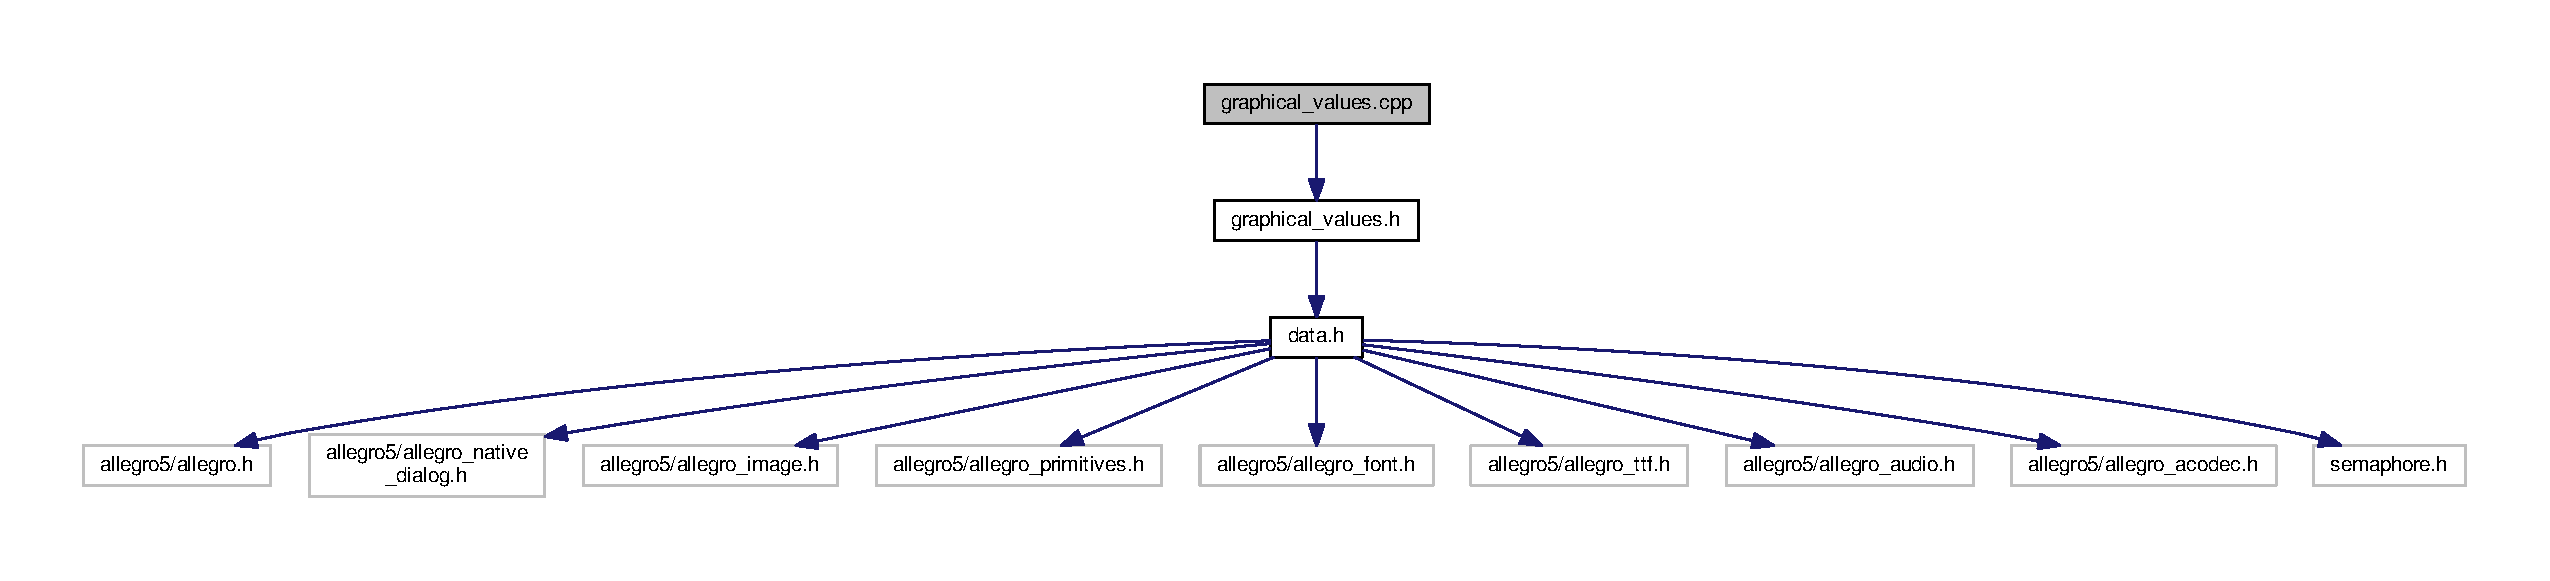
\includegraphics[width=350pt]{d1/d2f/graphical__values_8cpp__incl}
\end{center}
\end{figure}
\subsection*{Funzioni}
\begin{DoxyCompactItemize}
\item 
void \hyperlink{graphical__values_8cpp_a4cfe1723d77e138cb1e822cc88670e56}{update\+\_\+graphical\+\_\+values} ()
\begin{DoxyCompactList}\small\item\em Aggiorna le proporzioni grafiche dei singoli oggetti in proporzione all\textquotesingle{}attuale dimensione del display. \end{DoxyCompactList}\end{DoxyCompactItemize}
\subsection*{Variabili}
\begin{DoxyCompactItemize}
\item 
\hyperlink{structgeneral__gv__t}{general\+\_\+gv\+\_\+t} \hyperlink{graphical__values_8cpp_aed9b611f5dc23d0c4b3423958ac92497}{G\+E\+N\+E\+R\+A\+L\+\_\+\+GV}
\begin{DoxyCompactList}\small\item\em Struct contenente le proporzioni grafiche generali. \end{DoxyCompactList}\item 
\hyperlink{structmenu__gv__t}{menu\+\_\+gv\+\_\+t} \hyperlink{graphical__values_8cpp_a8050b794d70ca38807298569dc1af9b1}{M\+E\+N\+U\+\_\+\+GV}
\begin{DoxyCompactList}\small\item\em Struct contenente le proporzioni grafiche dei menu. \end{DoxyCompactList}\item 
\hyperlink{structplaywa__gv__t}{playwa\+\_\+gv\+\_\+t} \hyperlink{graphical__values_8cpp_a38bfadb0325688402bf1999301ca2a1b}{P\+L\+A\+Y\+W\+A\+\_\+\+GV}
\begin{DoxyCompactList}\small\item\em Struct contenente le proporzioni grafiche della schermata di gioco. \end{DoxyCompactList}\item 
\hyperlink{structinstr__gv__t}{instr\+\_\+gv\+\_\+t} \hyperlink{graphical__values_8cpp_a19a4da312ef3ea2a005acbce135d96fd}{I\+N\+S\+T\+R\+\_\+\+GV}
\begin{DoxyCompactList}\small\item\em Struct contenente le proporzioni grafiche della schermata di pausa. \end{DoxyCompactList}\item 
\hyperlink{structusr__gv__t}{usr\+\_\+gv\+\_\+t} \hyperlink{graphical__values_8cpp_aba4a0deff6c9de510c6621913ab2a406}{U\+S\+R\+\_\+\+GV}
\begin{DoxyCompactList}\small\item\em Struct contenente le proporzioni grafiche della schermata di fine partita. \end{DoxyCompactList}\end{DoxyCompactItemize}


\subsection{Documentazione delle funzioni}
\mbox{\Hypertarget{graphical__values_8cpp_a4cfe1723d77e138cb1e822cc88670e56}\label{graphical__values_8cpp_a4cfe1723d77e138cb1e822cc88670e56}} 
\index{graphical\+\_\+values.\+cpp@{graphical\+\_\+values.\+cpp}!update\+\_\+graphical\+\_\+values@{update\+\_\+graphical\+\_\+values}}
\index{update\+\_\+graphical\+\_\+values@{update\+\_\+graphical\+\_\+values}!graphical\+\_\+values.\+cpp@{graphical\+\_\+values.\+cpp}}
\subsubsection{\texorpdfstring{update\+\_\+graphical\+\_\+values()}{update\_graphical\_values()}}
{\footnotesize\ttfamily void update\+\_\+graphical\+\_\+values (\begin{DoxyParamCaption}{ }\end{DoxyParamCaption})}



Aggiorna le proporzioni grafiche dei singoli oggetti in proporzione all\textquotesingle{}attuale dimensione del display. 



\subsection{Documentazione delle variabili}
\mbox{\Hypertarget{graphical__values_8cpp_aed9b611f5dc23d0c4b3423958ac92497}\label{graphical__values_8cpp_aed9b611f5dc23d0c4b3423958ac92497}} 
\index{graphical\+\_\+values.\+cpp@{graphical\+\_\+values.\+cpp}!G\+E\+N\+E\+R\+A\+L\+\_\+\+GV@{G\+E\+N\+E\+R\+A\+L\+\_\+\+GV}}
\index{G\+E\+N\+E\+R\+A\+L\+\_\+\+GV@{G\+E\+N\+E\+R\+A\+L\+\_\+\+GV}!graphical\+\_\+values.\+cpp@{graphical\+\_\+values.\+cpp}}
\subsubsection{\texorpdfstring{G\+E\+N\+E\+R\+A\+L\+\_\+\+GV}{GENERAL\_GV}}
{\footnotesize\ttfamily \hyperlink{structgeneral__gv__t}{general\+\_\+gv\+\_\+t} G\+E\+N\+E\+R\+A\+L\+\_\+\+GV}



Struct contenente le proporzioni grafiche generali. 

\mbox{\Hypertarget{graphical__values_8cpp_a19a4da312ef3ea2a005acbce135d96fd}\label{graphical__values_8cpp_a19a4da312ef3ea2a005acbce135d96fd}} 
\index{graphical\+\_\+values.\+cpp@{graphical\+\_\+values.\+cpp}!I\+N\+S\+T\+R\+\_\+\+GV@{I\+N\+S\+T\+R\+\_\+\+GV}}
\index{I\+N\+S\+T\+R\+\_\+\+GV@{I\+N\+S\+T\+R\+\_\+\+GV}!graphical\+\_\+values.\+cpp@{graphical\+\_\+values.\+cpp}}
\subsubsection{\texorpdfstring{I\+N\+S\+T\+R\+\_\+\+GV}{INSTR\_GV}}
{\footnotesize\ttfamily \hyperlink{structinstr__gv__t}{instr\+\_\+gv\+\_\+t} I\+N\+S\+T\+R\+\_\+\+GV}



Struct contenente le proporzioni grafiche della schermata di pausa. 

\mbox{\Hypertarget{graphical__values_8cpp_a8050b794d70ca38807298569dc1af9b1}\label{graphical__values_8cpp_a8050b794d70ca38807298569dc1af9b1}} 
\index{graphical\+\_\+values.\+cpp@{graphical\+\_\+values.\+cpp}!M\+E\+N\+U\+\_\+\+GV@{M\+E\+N\+U\+\_\+\+GV}}
\index{M\+E\+N\+U\+\_\+\+GV@{M\+E\+N\+U\+\_\+\+GV}!graphical\+\_\+values.\+cpp@{graphical\+\_\+values.\+cpp}}
\subsubsection{\texorpdfstring{M\+E\+N\+U\+\_\+\+GV}{MENU\_GV}}
{\footnotesize\ttfamily \hyperlink{structmenu__gv__t}{menu\+\_\+gv\+\_\+t} M\+E\+N\+U\+\_\+\+GV}



Struct contenente le proporzioni grafiche dei menu. 

\mbox{\Hypertarget{graphical__values_8cpp_a38bfadb0325688402bf1999301ca2a1b}\label{graphical__values_8cpp_a38bfadb0325688402bf1999301ca2a1b}} 
\index{graphical\+\_\+values.\+cpp@{graphical\+\_\+values.\+cpp}!P\+L\+A\+Y\+W\+A\+\_\+\+GV@{P\+L\+A\+Y\+W\+A\+\_\+\+GV}}
\index{P\+L\+A\+Y\+W\+A\+\_\+\+GV@{P\+L\+A\+Y\+W\+A\+\_\+\+GV}!graphical\+\_\+values.\+cpp@{graphical\+\_\+values.\+cpp}}
\subsubsection{\texorpdfstring{P\+L\+A\+Y\+W\+A\+\_\+\+GV}{PLAYWA\_GV}}
{\footnotesize\ttfamily \hyperlink{structplaywa__gv__t}{playwa\+\_\+gv\+\_\+t} P\+L\+A\+Y\+W\+A\+\_\+\+GV}



Struct contenente le proporzioni grafiche della schermata di gioco. 

\mbox{\Hypertarget{graphical__values_8cpp_aba4a0deff6c9de510c6621913ab2a406}\label{graphical__values_8cpp_aba4a0deff6c9de510c6621913ab2a406}} 
\index{graphical\+\_\+values.\+cpp@{graphical\+\_\+values.\+cpp}!U\+S\+R\+\_\+\+GV@{U\+S\+R\+\_\+\+GV}}
\index{U\+S\+R\+\_\+\+GV@{U\+S\+R\+\_\+\+GV}!graphical\+\_\+values.\+cpp@{graphical\+\_\+values.\+cpp}}
\subsubsection{\texorpdfstring{U\+S\+R\+\_\+\+GV}{USR\_GV}}
{\footnotesize\ttfamily \hyperlink{structusr__gv__t}{usr\+\_\+gv\+\_\+t} U\+S\+R\+\_\+\+GV}



Struct contenente le proporzioni grafiche della schermata di fine partita. 


\hypertarget{graphical__values_8h}{}\section{Riferimenti per il file graphical\+\_\+values.\+h}
\label{graphical__values_8h}\index{graphical\+\_\+values.\+h@{graphical\+\_\+values.\+h}}
{\ttfamily \#include \char`\"{}data.\+h\char`\"{}}\newline
Grafo delle dipendenze di inclusione per graphical\+\_\+values.\+h\+:\nopagebreak
\begin{figure}[H]
\begin{center}
\leavevmode
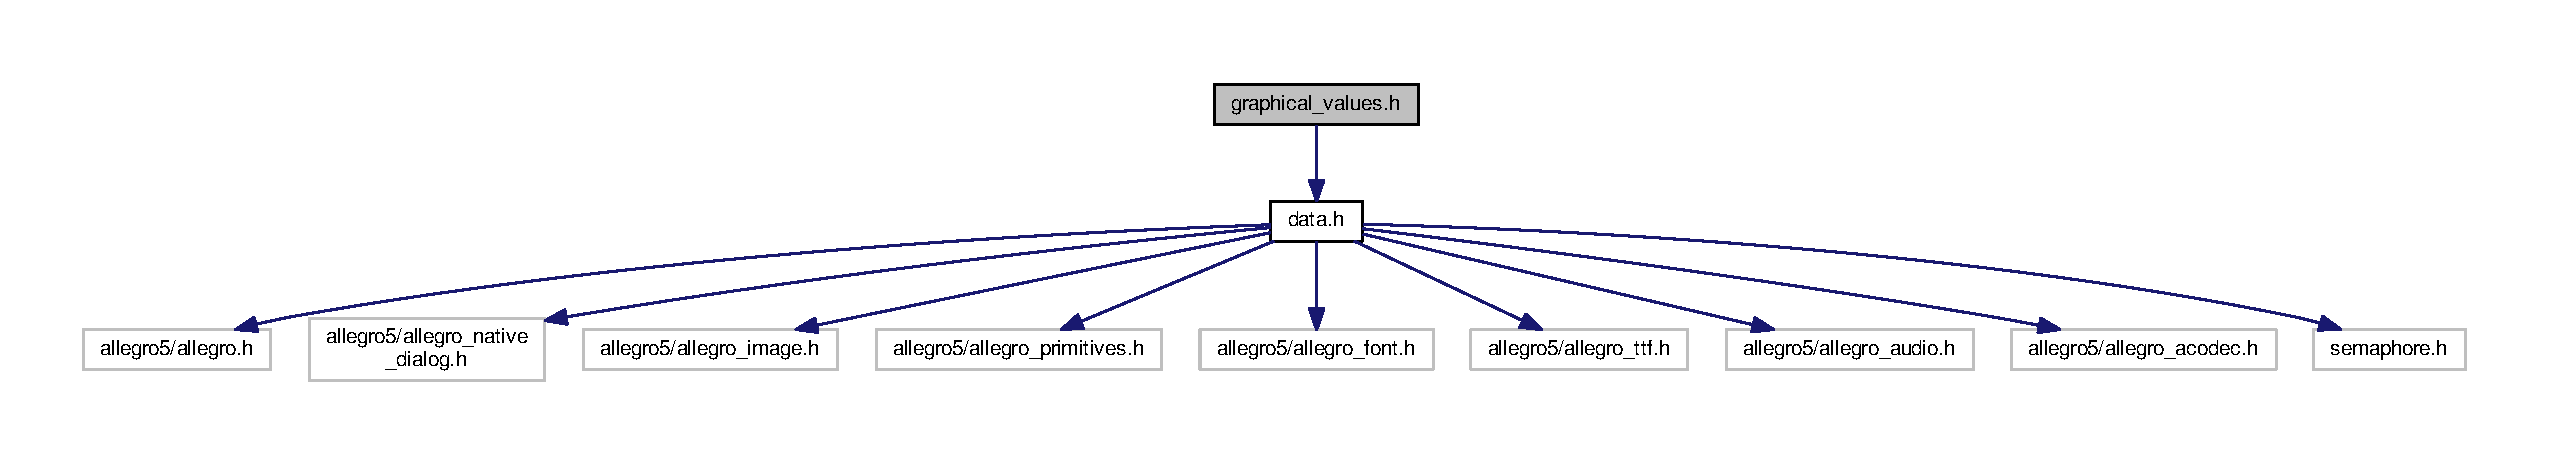
\includegraphics[width=350pt]{d4/d21/graphical__values_8h__incl}
\end{center}
\end{figure}
Questo grafo mostra quali altri file includono direttamente o indirettamente questo file\+:\nopagebreak
\begin{figure}[H]
\begin{center}
\leavevmode
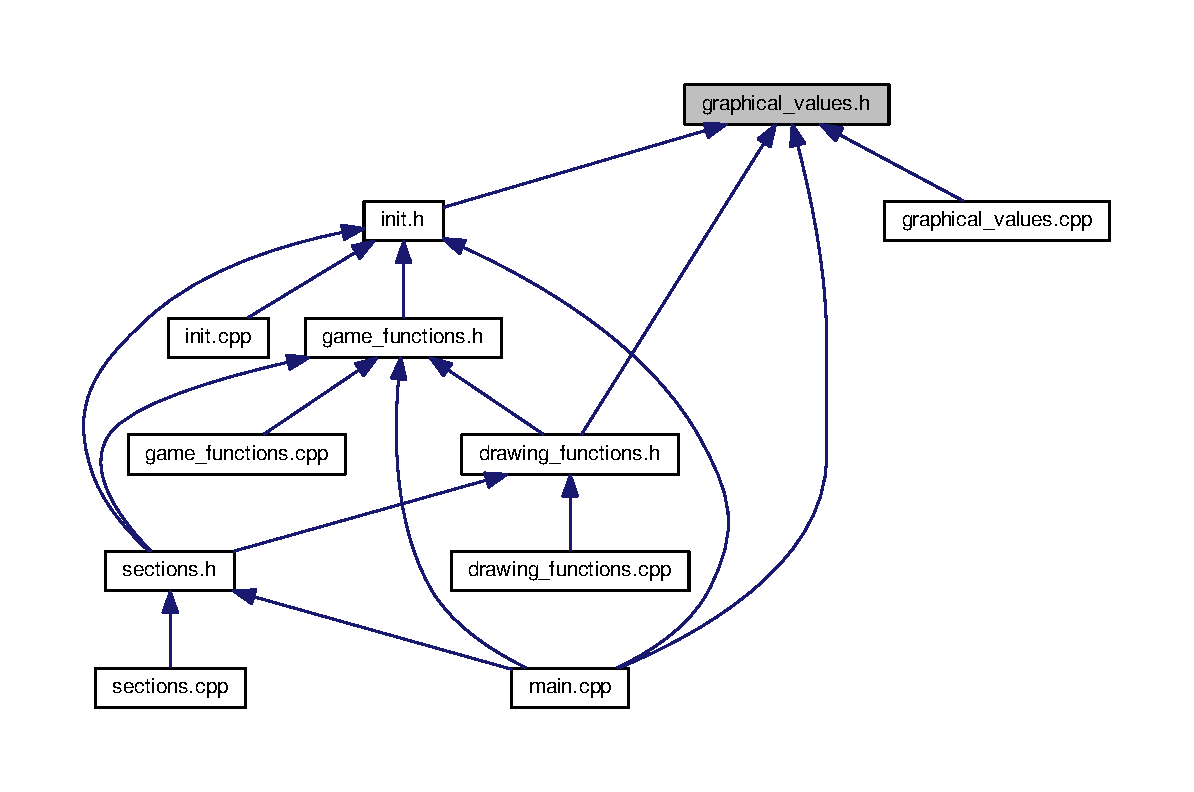
\includegraphics[width=350pt]{d1/d43/graphical__values_8h__dep__incl}
\end{center}
\end{figure}
\subsection*{Funzioni}
\begin{DoxyCompactItemize}
\item 
void \hyperlink{graphical__values_8h_a4cfe1723d77e138cb1e822cc88670e56}{update\+\_\+graphical\+\_\+values} ()
\begin{DoxyCompactList}\small\item\em Aggiorna le proporzioni grafiche dei singoli oggetti in proporzione all\textquotesingle{}attuale dimensione del display. \end{DoxyCompactList}\end{DoxyCompactItemize}
\subsection*{Variabili}
\begin{DoxyCompactItemize}
\item 
\hyperlink{structdisplay__info__t}{display\+\_\+info\+\_\+t} \hyperlink{graphical__values_8h_a781a8df874545e4f5bff5f8a446d1963}{display\+\_\+info}
\end{DoxyCompactItemize}


\subsection{Documentazione delle funzioni}
\mbox{\Hypertarget{graphical__values_8h_a4cfe1723d77e138cb1e822cc88670e56}\label{graphical__values_8h_a4cfe1723d77e138cb1e822cc88670e56}} 
\index{graphical\+\_\+values.\+h@{graphical\+\_\+values.\+h}!update\+\_\+graphical\+\_\+values@{update\+\_\+graphical\+\_\+values}}
\index{update\+\_\+graphical\+\_\+values@{update\+\_\+graphical\+\_\+values}!graphical\+\_\+values.\+h@{graphical\+\_\+values.\+h}}
\subsubsection{\texorpdfstring{update\+\_\+graphical\+\_\+values()}{update\_graphical\_values()}}
{\footnotesize\ttfamily void update\+\_\+graphical\+\_\+values (\begin{DoxyParamCaption}{ }\end{DoxyParamCaption})}



Aggiorna le proporzioni grafiche dei singoli oggetti in proporzione all\textquotesingle{}attuale dimensione del display. 



\subsection{Documentazione delle variabili}
\mbox{\Hypertarget{graphical__values_8h_a781a8df874545e4f5bff5f8a446d1963}\label{graphical__values_8h_a781a8df874545e4f5bff5f8a446d1963}} 
\index{graphical\+\_\+values.\+h@{graphical\+\_\+values.\+h}!display\+\_\+info@{display\+\_\+info}}
\index{display\+\_\+info@{display\+\_\+info}!graphical\+\_\+values.\+h@{graphical\+\_\+values.\+h}}
\subsubsection{\texorpdfstring{display\+\_\+info}{display\_info}}
{\footnotesize\ttfamily \hyperlink{structdisplay__info__t}{display\+\_\+info\+\_\+t} display\+\_\+info}


\hypertarget{init_8cpp}{}\section{Riferimenti per il file init.\+cpp}
\label{init_8cpp}\index{init.\+cpp@{init.\+cpp}}
{\ttfamily \#include \char`\"{}init.\+h\char`\"{}}\newline
Grafo delle dipendenze di inclusione per init.\+cpp\+:\nopagebreak
\begin{figure}[H]
\begin{center}
\leavevmode
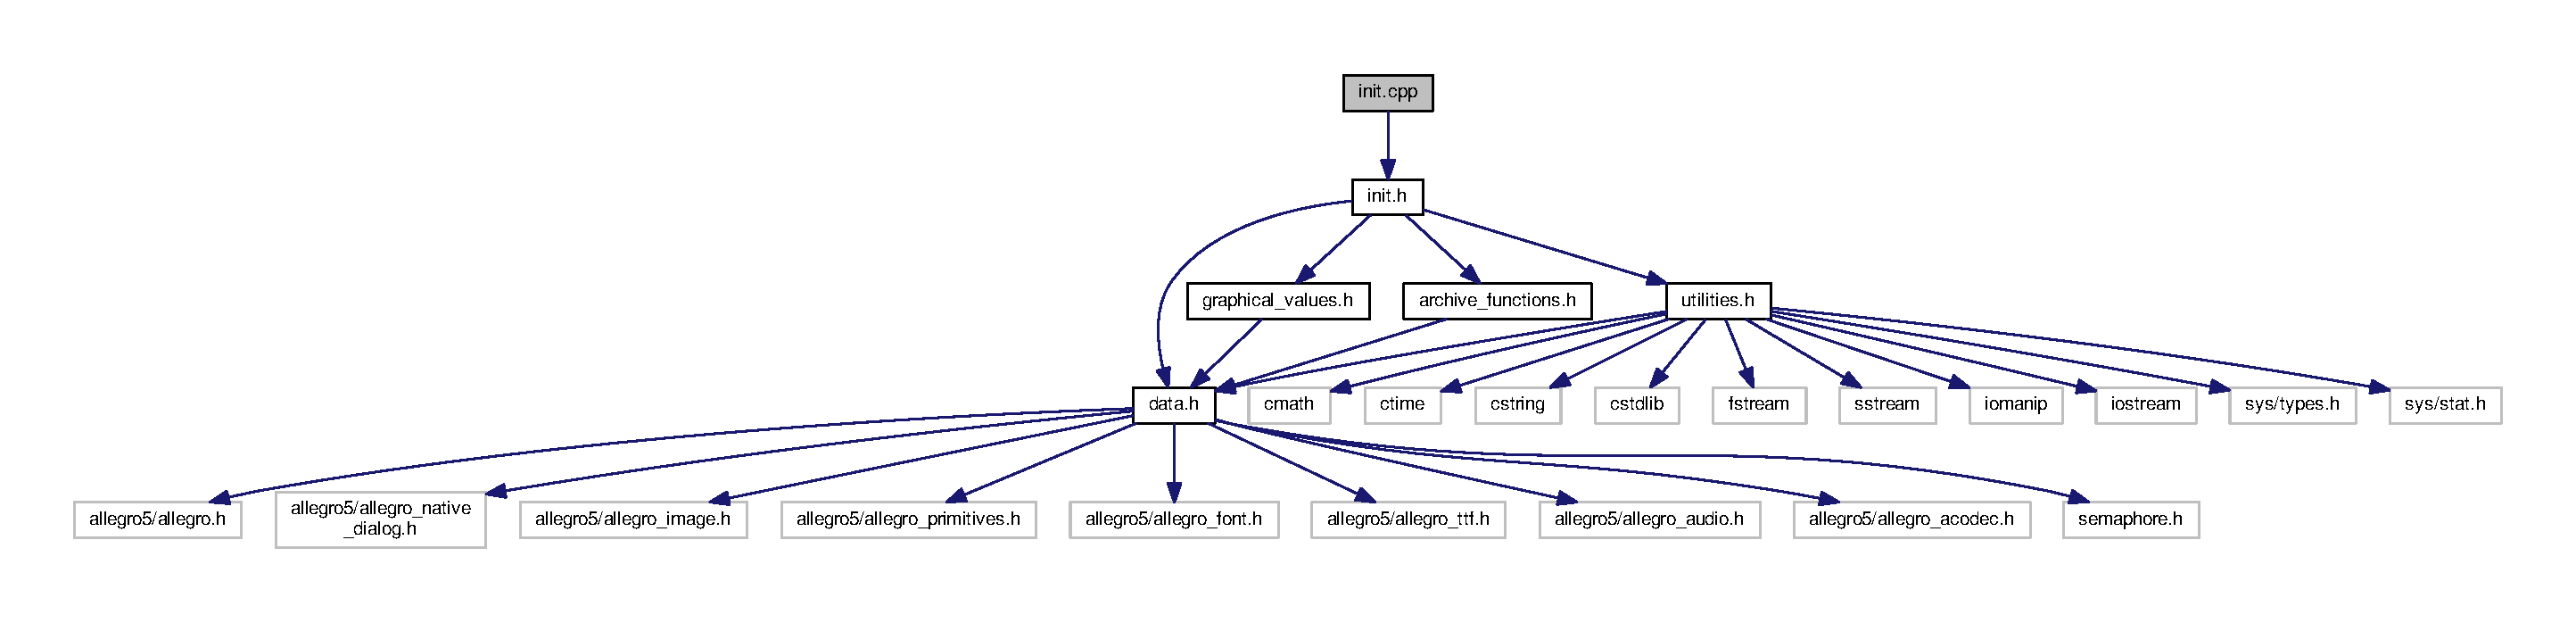
\includegraphics[width=350pt]{df/d07/init_8cpp__incl}
\end{center}
\end{figure}
\subsection*{Funzioni}
\begin{DoxyCompactItemize}
\item 
void \hyperlink{init_8cpp_ac163c1a07df84ea573bc8193ef0b1d4d}{sort\+\_\+file\+\_\+list} (\hyperlink{structls__t}{ls\+\_\+t} $\ast$file\+\_\+list)
\begin{DoxyCompactList}\small\item\em Funzione che ordina un array di elementi che rappresentano gli archivi in ordine crescente in base alla loro dimensione. \end{DoxyCompactList}\item 
bool \hyperlink{init_8cpp_ad344b8e4aa48698e5e02723af7cb9cf3}{init\+\_\+game\+\_\+requirements} ()
\begin{DoxyCompactList}\small\item\em Funzione che inizializza le funzionalità relative all\textquotesingle{}audio, ai font (ttf), alla tastiera. \end{DoxyCompactList}\item 
\hyperlink{structdisplay__info__t}{display\+\_\+info\+\_\+t} \hyperlink{init_8cpp_a52af8e422d4613b6d748fe26befa48fe}{init\+\_\+display\+\_\+res} ()
\begin{DoxyCompactList}\small\item\em Funzione che inizializza le dimensioni del display di gioco in base alle proporzioni standard (1280x800), adattandole al monitor del proprio computer. \end{DoxyCompactList}\item 
void \hyperlink{init_8cpp_a026a4c3b4000d2f08220df0d54f61f5a}{init\+\_\+display} (A\+L\+L\+E\+G\+R\+O\+\_\+\+D\+I\+S\+P\+L\+AY $\ast$\&display)
\begin{DoxyCompactList}\small\item\em Funzione che crea il display ed inizializza il titolo e l\textquotesingle{}icona. \end{DoxyCompactList}\item 
A\+L\+L\+E\+G\+R\+O\+\_\+\+E\+V\+E\+N\+T\+\_\+\+Q\+U\+E\+UE $\ast$ \hyperlink{init_8cpp_a5059121608a64d2b96b2d3a95816213e}{init\+\_\+queue\+\_\+event} (A\+L\+L\+E\+G\+R\+O\+\_\+\+D\+I\+S\+P\+L\+AY $\ast$\&display)
\begin{DoxyCompactList}\small\item\em Funzione che crea il puntatore alla coda degli eventi e aggancia alla coda gli eventi relativi alla tastiera e display. \end{DoxyCompactList}\item 
int \hyperlink{init_8cpp_ae891066631b0f2207f9781f0e96ed154}{init\+\_\+target\+\_\+bonus} (int \&instant\+\_\+ast\+\_\+dest, const int \&asteroids\+\_\+destroyed)
\begin{DoxyCompactList}\small\item\em Funzione che indica dopo quanti asteroidi distrutti ottengo il bonus. \end{DoxyCompactList}\item 
A\+L\+L\+E\+G\+R\+O\+\_\+\+S\+A\+M\+P\+LE $\ast$ \hyperlink{init_8cpp_ae3a65cb2bb1a457481b60f2417f13f8c}{init\+\_\+sound\+\_\+music} (const char $\ast$path)
\begin{DoxyCompactList}\small\item\em Funzione che inizializza un suono del gioco. \end{DoxyCompactList}\item 
void \hyperlink{init_8cpp_a5631504bde981afe8e70db1895d14477}{init\+\_\+match\+\_\+vars} (\hyperlink{structmatch__vars__t}{match\+\_\+vars\+\_\+t} \&match\+\_\+vars, A\+L\+L\+E\+G\+R\+O\+\_\+\+E\+V\+E\+N\+T\+\_\+\+Q\+U\+E\+UE $\ast$ev\+\_\+queue)
\begin{DoxyCompactList}\small\item\em Funzione che inizializza le varaibili di gioco. \end{DoxyCompactList}\item 
void \hyperlink{init_8cpp_a5999157721faf925c4822d402870417c}{init\+\_\+settings} (\hyperlink{structsettings__t}{settings\+\_\+t} \&settings)
\begin{DoxyCompactList}\small\item\em Funzione che inizializza le impostazioni di gioco. \end{DoxyCompactList}\item 
void \hyperlink{init_8cpp_a560d5e5345170bf7a0ba01f2e1cb70c8}{init\+\_\+shooter} (\hyperlink{structshooter__t}{shooter\+\_\+t} \&shooter)
\begin{DoxyCompactList}\small\item\em Funzione che inizializza le informazioni dello shooter a inizio gioco. \end{DoxyCompactList}\item 
void \hyperlink{init_8cpp_a40954ccd9e8a0df2e11b3354d3a64ad5}{init\+\_\+bullet} (\hyperlink{structbullet__t}{bullet\+\_\+t} \&bullet)
\begin{DoxyCompactList}\small\item\em Funzione che inizializza le informazioni di un proiettile. \end{DoxyCompactList}\item 
void \hyperlink{init_8cpp_adb1bf0e82cb52f3294b65aa78b849171}{init\+\_\+arr\+\_\+bullet} (\hyperlink{structbullet__t}{bullet\+\_\+t} $\ast$arr\+\_\+bullet)
\begin{DoxyCompactList}\small\item\em Funzione che inizializza un array di puntatori a asteroidi. \end{DoxyCompactList}\item 
void \hyperlink{init_8cpp_a15a7313c1fbdd2555dda976bd9a8a1e2}{init\+\_\+words\+\_\+buffer} (\hyperlink{structwords__buffer__t}{words\+\_\+buffer\+\_\+t} \&\hyperlink{sections_8h_aaa25f9883d8c134861353b1bf5e00846}{words\+\_\+buffer})
\begin{DoxyCompactList}\small\item\em Funzione che inizializza l\textquotesingle{}array utilizzato come buffer per le parole tra producer e consumer. \end{DoxyCompactList}\item 
void \hyperlink{init_8cpp_afcfd631f7a107270b7786218d6a08bb1}{init\+\_\+thread\+\_\+manager} (\hyperlink{structthread__manager__t}{thread\+\_\+manager\+\_\+t} \&\hyperlink{sections_8h_ad04f177b84df22adea5536cbae88451b}{thread\+\_\+manager}, char $\ast$email)
\begin{DoxyCompactList}\small\item\em Funzione che inizializza la struttura dati del thread manager. \end{DoxyCompactList}\end{DoxyCompactItemize}


\subsection{Documentazione delle funzioni}
\mbox{\Hypertarget{init_8cpp_adb1bf0e82cb52f3294b65aa78b849171}\label{init_8cpp_adb1bf0e82cb52f3294b65aa78b849171}} 
\index{init.\+cpp@{init.\+cpp}!init\+\_\+arr\+\_\+bullet@{init\+\_\+arr\+\_\+bullet}}
\index{init\+\_\+arr\+\_\+bullet@{init\+\_\+arr\+\_\+bullet}!init.\+cpp@{init.\+cpp}}
\subsubsection{\texorpdfstring{init\+\_\+arr\+\_\+bullet()}{init\_arr\_bullet()}}
{\footnotesize\ttfamily void init\+\_\+arr\+\_\+bullet (\begin{DoxyParamCaption}\item[{\hyperlink{structbullet__t}{bullet\+\_\+t} $\ast$}]{arr\+\_\+bullet }\end{DoxyParamCaption})}



Funzione che inizializza un array di puntatori a asteroidi. 

~\newline
Parametri\+: ~\newline
1) arr\+\_\+bullet -\/ Array dei bullet. \mbox{\Hypertarget{init_8cpp_a40954ccd9e8a0df2e11b3354d3a64ad5}\label{init_8cpp_a40954ccd9e8a0df2e11b3354d3a64ad5}} 
\index{init.\+cpp@{init.\+cpp}!init\+\_\+bullet@{init\+\_\+bullet}}
\index{init\+\_\+bullet@{init\+\_\+bullet}!init.\+cpp@{init.\+cpp}}
\subsubsection{\texorpdfstring{init\+\_\+bullet()}{init\_bullet()}}
{\footnotesize\ttfamily void init\+\_\+bullet (\begin{DoxyParamCaption}\item[{\hyperlink{structbullet__t}{bullet\+\_\+t} \&}]{bullet }\end{DoxyParamCaption})}



Funzione che inizializza le informazioni di un proiettile. 

~\newline
Parametri\+: ~\newline
1) shooter -\/ Struct relativo al singolo proiettile. \mbox{\Hypertarget{init_8cpp_a026a4c3b4000d2f08220df0d54f61f5a}\label{init_8cpp_a026a4c3b4000d2f08220df0d54f61f5a}} 
\index{init.\+cpp@{init.\+cpp}!init\+\_\+display@{init\+\_\+display}}
\index{init\+\_\+display@{init\+\_\+display}!init.\+cpp@{init.\+cpp}}
\subsubsection{\texorpdfstring{init\+\_\+display()}{init\_display()}}
{\footnotesize\ttfamily void init\+\_\+display (\begin{DoxyParamCaption}\item[{A\+L\+L\+E\+G\+R\+O\+\_\+\+D\+I\+S\+P\+L\+AY $\ast$\&}]{display }\end{DoxyParamCaption})}



Funzione che crea il display ed inizializza il titolo e l\textquotesingle{}icona. 

~\newline
Parametri\+: ~\newline
1) display -\/ Puntatore al display del gioco; ~\newline
\mbox{\Hypertarget{init_8cpp_a52af8e422d4613b6d748fe26befa48fe}\label{init_8cpp_a52af8e422d4613b6d748fe26befa48fe}} 
\index{init.\+cpp@{init.\+cpp}!init\+\_\+display\+\_\+res@{init\+\_\+display\+\_\+res}}
\index{init\+\_\+display\+\_\+res@{init\+\_\+display\+\_\+res}!init.\+cpp@{init.\+cpp}}
\subsubsection{\texorpdfstring{init\+\_\+display\+\_\+res()}{init\_display\_res()}}
{\footnotesize\ttfamily \hyperlink{structdisplay__info__t}{display\+\_\+info\+\_\+t} init\+\_\+display\+\_\+res (\begin{DoxyParamCaption}{ }\end{DoxyParamCaption})}



Funzione che inizializza le dimensioni del display di gioco in base alle proporzioni standard (1280x800), adattandole al monitor del proprio computer. 

Viene lasciata libera una certa porzione di schermo (1/5 in altezza). ~\newline
Ritorna le dimensioni effettive del display di gioco. \mbox{\Hypertarget{init_8cpp_ad344b8e4aa48698e5e02723af7cb9cf3}\label{init_8cpp_ad344b8e4aa48698e5e02723af7cb9cf3}} 
\index{init.\+cpp@{init.\+cpp}!init\+\_\+game\+\_\+requirements@{init\+\_\+game\+\_\+requirements}}
\index{init\+\_\+game\+\_\+requirements@{init\+\_\+game\+\_\+requirements}!init.\+cpp@{init.\+cpp}}
\subsubsection{\texorpdfstring{init\+\_\+game\+\_\+requirements()}{init\_game\_requirements()}}
{\footnotesize\ttfamily bool init\+\_\+game\+\_\+requirements (\begin{DoxyParamCaption}{ }\end{DoxyParamCaption})}



Funzione che inizializza le funzionalità relative all\textquotesingle{}audio, ai font (ttf), alla tastiera. 

~\newline
Ritorna un booleano che indica il successo delle installazioni. \mbox{\Hypertarget{init_8cpp_a5631504bde981afe8e70db1895d14477}\label{init_8cpp_a5631504bde981afe8e70db1895d14477}} 
\index{init.\+cpp@{init.\+cpp}!init\+\_\+match\+\_\+vars@{init\+\_\+match\+\_\+vars}}
\index{init\+\_\+match\+\_\+vars@{init\+\_\+match\+\_\+vars}!init.\+cpp@{init.\+cpp}}
\subsubsection{\texorpdfstring{init\+\_\+match\+\_\+vars()}{init\_match\_vars()}}
{\footnotesize\ttfamily void init\+\_\+match\+\_\+vars (\begin{DoxyParamCaption}\item[{\hyperlink{structmatch__vars__t}{match\+\_\+vars\+\_\+t} \&}]{match\+\_\+vars,  }\item[{A\+L\+L\+E\+G\+R\+O\+\_\+\+E\+V\+E\+N\+T\+\_\+\+Q\+U\+E\+UE $\ast$}]{ev\+\_\+queue }\end{DoxyParamCaption})}



Funzione che inizializza le varaibili di gioco. 

~\newline
Parametri\+: ~\newline
1) match\+\_\+vars -\/ Struct contenente le variabili di gioco; 2) ev\+\_\+queue -\/ Coda degli eventi (per inizializzazione dei timer). \mbox{\Hypertarget{init_8cpp_a5059121608a64d2b96b2d3a95816213e}\label{init_8cpp_a5059121608a64d2b96b2d3a95816213e}} 
\index{init.\+cpp@{init.\+cpp}!init\+\_\+queue\+\_\+event@{init\+\_\+queue\+\_\+event}}
\index{init\+\_\+queue\+\_\+event@{init\+\_\+queue\+\_\+event}!init.\+cpp@{init.\+cpp}}
\subsubsection{\texorpdfstring{init\+\_\+queue\+\_\+event()}{init\_queue\_event()}}
{\footnotesize\ttfamily A\+L\+L\+E\+G\+R\+O\+\_\+\+E\+V\+E\+N\+T\+\_\+\+Q\+U\+E\+UE$\ast$ init\+\_\+queue\+\_\+event (\begin{DoxyParamCaption}\item[{A\+L\+L\+E\+G\+R\+O\+\_\+\+D\+I\+S\+P\+L\+AY $\ast$\&}]{display }\end{DoxyParamCaption})}



Funzione che crea il puntatore alla coda degli eventi e aggancia alla coda gli eventi relativi alla tastiera e display. 

~\newline
Parametri\+: ~\newline
1) display -\/ Puntatore al display del gioco; ~\newline
Ritorna il puntatore alla coda del display, o nullptr se si è verificato un errore nella creazione. \mbox{\Hypertarget{init_8cpp_a5999157721faf925c4822d402870417c}\label{init_8cpp_a5999157721faf925c4822d402870417c}} 
\index{init.\+cpp@{init.\+cpp}!init\+\_\+settings@{init\+\_\+settings}}
\index{init\+\_\+settings@{init\+\_\+settings}!init.\+cpp@{init.\+cpp}}
\subsubsection{\texorpdfstring{init\+\_\+settings()}{init\_settings()}}
{\footnotesize\ttfamily void init\+\_\+settings (\begin{DoxyParamCaption}\item[{\hyperlink{structsettings__t}{settings\+\_\+t} \&}]{settings }\end{DoxyParamCaption})}



Funzione che inizializza le impostazioni di gioco. 

~\newline
Parametri\+: ~\newline
1) settings -\/ Struct contenente le impostazioni di gioco. \mbox{\Hypertarget{init_8cpp_a560d5e5345170bf7a0ba01f2e1cb70c8}\label{init_8cpp_a560d5e5345170bf7a0ba01f2e1cb70c8}} 
\index{init.\+cpp@{init.\+cpp}!init\+\_\+shooter@{init\+\_\+shooter}}
\index{init\+\_\+shooter@{init\+\_\+shooter}!init.\+cpp@{init.\+cpp}}
\subsubsection{\texorpdfstring{init\+\_\+shooter()}{init\_shooter()}}
{\footnotesize\ttfamily void init\+\_\+shooter (\begin{DoxyParamCaption}\item[{\hyperlink{structshooter__t}{shooter\+\_\+t} \&}]{shooter }\end{DoxyParamCaption})}



Funzione che inizializza le informazioni dello shooter a inizio gioco. 

~\newline
Parametri\+: ~\newline
1) shooter -\/ Struct relativo alla navicella. \mbox{\Hypertarget{init_8cpp_ae3a65cb2bb1a457481b60f2417f13f8c}\label{init_8cpp_ae3a65cb2bb1a457481b60f2417f13f8c}} 
\index{init.\+cpp@{init.\+cpp}!init\+\_\+sound\+\_\+music@{init\+\_\+sound\+\_\+music}}
\index{init\+\_\+sound\+\_\+music@{init\+\_\+sound\+\_\+music}!init.\+cpp@{init.\+cpp}}
\subsubsection{\texorpdfstring{init\+\_\+sound\+\_\+music()}{init\_sound\_music()}}
{\footnotesize\ttfamily A\+L\+L\+E\+G\+R\+O\+\_\+\+S\+A\+M\+P\+LE$\ast$ init\+\_\+sound\+\_\+music (\begin{DoxyParamCaption}\item[{const char $\ast$}]{path }\end{DoxyParamCaption})}



Funzione che inizializza un suono del gioco. 

Le impostazioni di inizializzazione sono standard, e il suono viene ripetuto una sola volta. ~\newline
Parametri\+: ~\newline
1) path -\/ Percorso del file audio; ~\newline
Ritorna il puntatore al suono inizializzato. \mbox{\Hypertarget{init_8cpp_ae891066631b0f2207f9781f0e96ed154}\label{init_8cpp_ae891066631b0f2207f9781f0e96ed154}} 
\index{init.\+cpp@{init.\+cpp}!init\+\_\+target\+\_\+bonus@{init\+\_\+target\+\_\+bonus}}
\index{init\+\_\+target\+\_\+bonus@{init\+\_\+target\+\_\+bonus}!init.\+cpp@{init.\+cpp}}
\subsubsection{\texorpdfstring{init\+\_\+target\+\_\+bonus()}{init\_target\_bonus()}}
{\footnotesize\ttfamily int init\+\_\+target\+\_\+bonus (\begin{DoxyParamCaption}\item[{int \&}]{instant\+\_\+ast\+\_\+dest,  }\item[{const int \&}]{asteroids\+\_\+destroyed }\end{DoxyParamCaption})}



Funzione che indica dopo quanti asteroidi distrutti ottengo il bonus. 

Inizializza instant\+\_\+ast\+\_\+dest, per memorizzare quanti asteroidi sono stati distrutti fino a quel momento, per controllare ad ogni asteroide distrutto se si ha diritto al bonus. ~\newline
Parametri\+: ~\newline
1) instant\+\_\+ast\+\_\+dest -\/ Appoggio per sapere quanti asteroidi ho distrutto in quel momento, per capire se ho raggiunto il bonus ~\newline
2) asteroids\+\_\+destroyed -\/ Numero di asteroidi distrutti in quel momento \mbox{\Hypertarget{init_8cpp_afcfd631f7a107270b7786218d6a08bb1}\label{init_8cpp_afcfd631f7a107270b7786218d6a08bb1}} 
\index{init.\+cpp@{init.\+cpp}!init\+\_\+thread\+\_\+manager@{init\+\_\+thread\+\_\+manager}}
\index{init\+\_\+thread\+\_\+manager@{init\+\_\+thread\+\_\+manager}!init.\+cpp@{init.\+cpp}}
\subsubsection{\texorpdfstring{init\+\_\+thread\+\_\+manager()}{init\_thread\_manager()}}
{\footnotesize\ttfamily void init\+\_\+thread\+\_\+manager (\begin{DoxyParamCaption}\item[{\hyperlink{structthread__manager__t}{thread\+\_\+manager\+\_\+t} \&}]{thread\+\_\+manager,  }\item[{char $\ast$}]{email }\end{DoxyParamCaption})}



Funzione che inizializza la struttura dati del thread manager. 

~\newline
Questa struttura contiene i mutex, le condition variable e i thread utilizzati durante il gioco, al fine di sincronizzare i vari worker. ~\newline
Parametri\+: ~\newline
1) thread\+\_\+manager -\/ Variabile contenente le strutture per la sincronizzazione; 2) email -\/ Email da cercare con cui viene inizializzato il search manager. \mbox{\Hypertarget{init_8cpp_a15a7313c1fbdd2555dda976bd9a8a1e2}\label{init_8cpp_a15a7313c1fbdd2555dda976bd9a8a1e2}} 
\index{init.\+cpp@{init.\+cpp}!init\+\_\+words\+\_\+buffer@{init\+\_\+words\+\_\+buffer}}
\index{init\+\_\+words\+\_\+buffer@{init\+\_\+words\+\_\+buffer}!init.\+cpp@{init.\+cpp}}
\subsubsection{\texorpdfstring{init\+\_\+words\+\_\+buffer()}{init\_words\_buffer()}}
{\footnotesize\ttfamily void init\+\_\+words\+\_\+buffer (\begin{DoxyParamCaption}\item[{\hyperlink{structwords__buffer__t}{words\+\_\+buffer\+\_\+t} \&}]{words\+\_\+buffer }\end{DoxyParamCaption})}



Funzione che inizializza l\textquotesingle{}array utilizzato come buffer per le parole tra producer e consumer. 

~\newline
Parametri\+: ~\newline
1) words\+\_\+buffer -\/ Buffer delle parole. \mbox{\Hypertarget{init_8cpp_ac163c1a07df84ea573bc8193ef0b1d4d}\label{init_8cpp_ac163c1a07df84ea573bc8193ef0b1d4d}} 
\index{init.\+cpp@{init.\+cpp}!sort\+\_\+file\+\_\+list@{sort\+\_\+file\+\_\+list}}
\index{sort\+\_\+file\+\_\+list@{sort\+\_\+file\+\_\+list}!init.\+cpp@{init.\+cpp}}
\subsubsection{\texorpdfstring{sort\+\_\+file\+\_\+list()}{sort\_file\_list()}}
{\footnotesize\ttfamily void sort\+\_\+file\+\_\+list (\begin{DoxyParamCaption}\item[{\hyperlink{structls__t}{ls\+\_\+t} $\ast$}]{file\+\_\+list }\end{DoxyParamCaption})}



Funzione che ordina un array di elementi che rappresentano gli archivi in ordine crescente in base alla loro dimensione. 

~\newline
Parametri\+: ~\newline
1) file\+\_\+list -\/ Lista degli archivi; ~\newline

\hypertarget{init_8h}{}\section{Riferimenti per il file init.\+h}
\label{init_8h}\index{init.\+h@{init.\+h}}
{\ttfamily \#include \char`\"{}data.\+h\char`\"{}}\newline
{\ttfamily \#include \char`\"{}graphical\+\_\+values.\+h\char`\"{}}\newline
{\ttfamily \#include \char`\"{}utilities.\+h\char`\"{}}\newline
{\ttfamily \#include \char`\"{}archive\+\_\+functions.\+h\char`\"{}}\newline
Grafo delle dipendenze di inclusione per init.\+h\+:\nopagebreak
\begin{figure}[H]
\begin{center}
\leavevmode
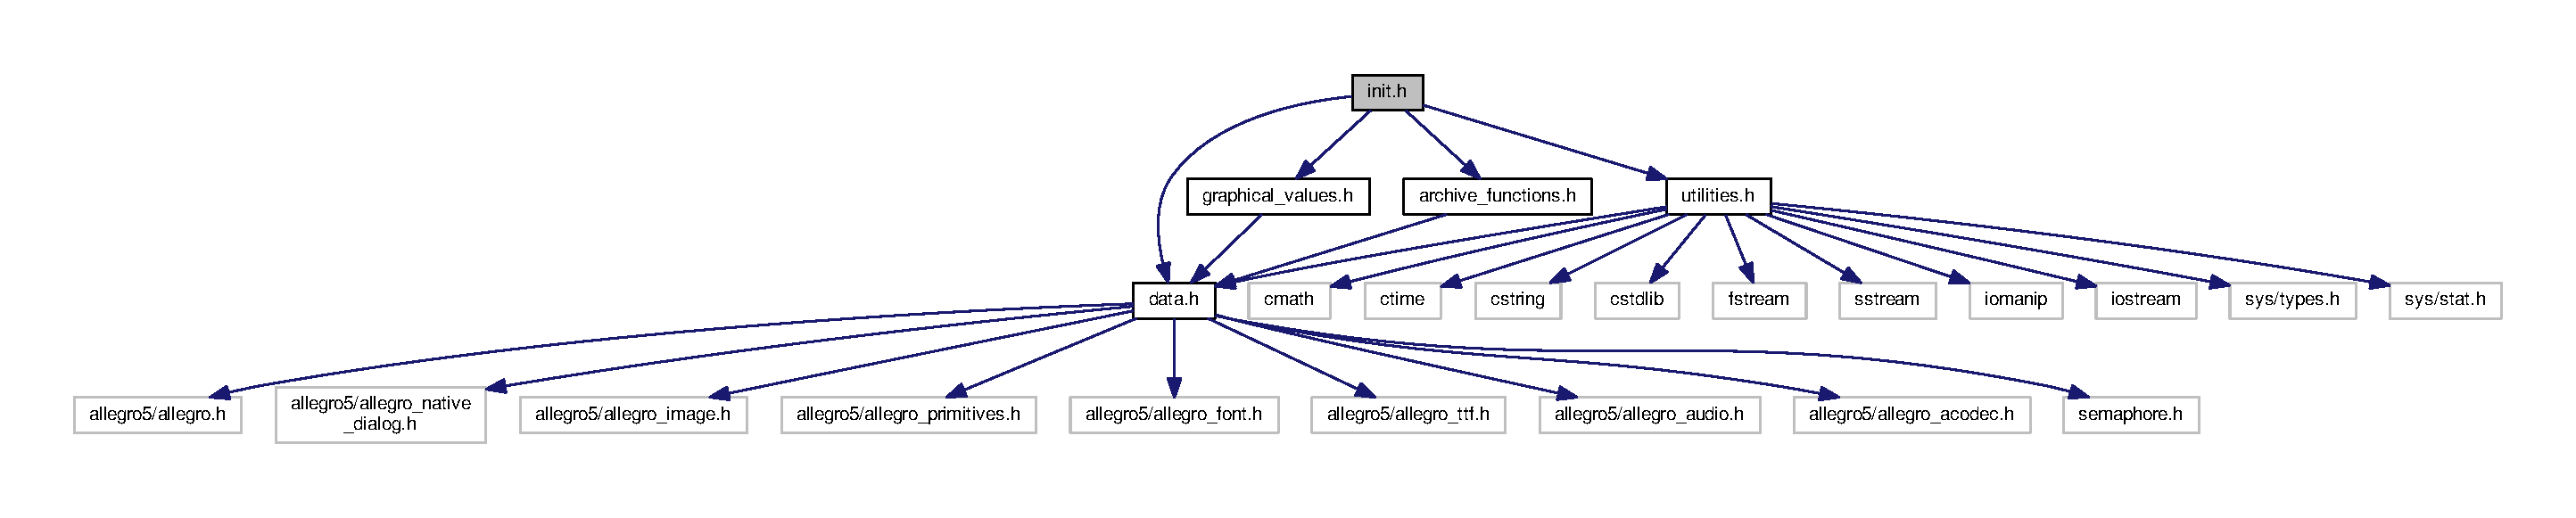
\includegraphics[width=350pt]{d3/dab/init_8h__incl}
\end{center}
\end{figure}
Questo grafo mostra quali altri file includono direttamente o indirettamente questo file\+:\nopagebreak
\begin{figure}[H]
\begin{center}
\leavevmode
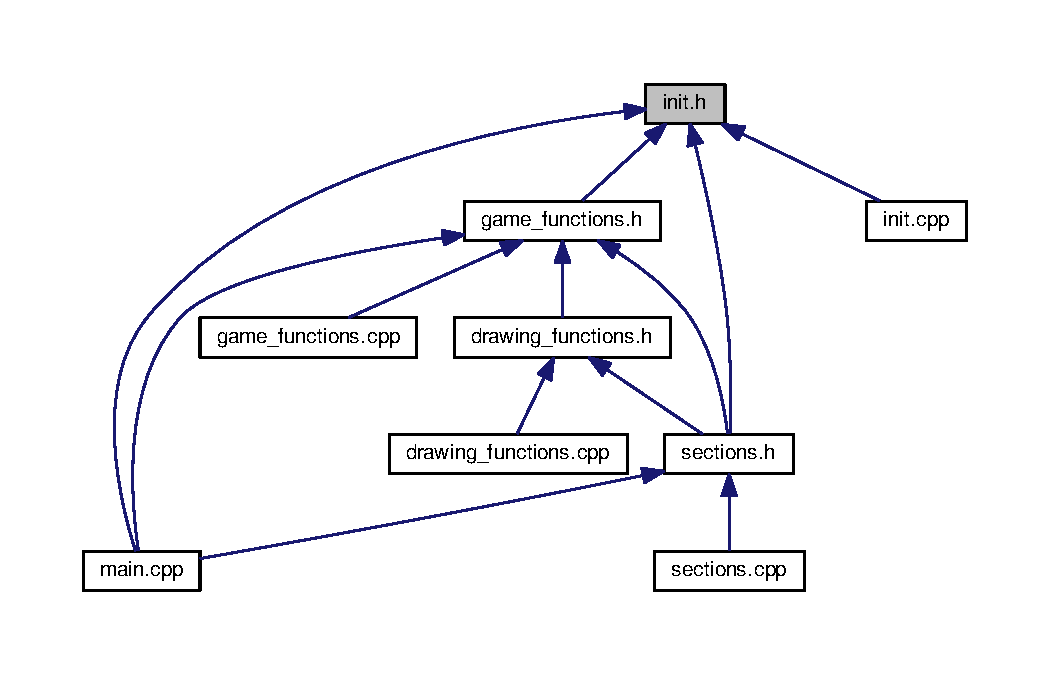
\includegraphics[width=350pt]{de/ddb/init_8h__dep__incl}
\end{center}
\end{figure}
\subsection*{Funzioni}
\begin{DoxyCompactItemize}
\item 
bool \hyperlink{init_8h_ad344b8e4aa48698e5e02723af7cb9cf3}{init\+\_\+game\+\_\+requirements} ()
\begin{DoxyCompactList}\small\item\em Funzione che inizializza le funzionalità relative all\textquotesingle{}audio, ai font (ttf), alla tastiera. \end{DoxyCompactList}\item 
\hyperlink{structdisplay__info__t}{display\+\_\+info\+\_\+t} \hyperlink{init_8h_a52af8e422d4613b6d748fe26befa48fe}{init\+\_\+display\+\_\+res} ()
\begin{DoxyCompactList}\small\item\em Funzione che inizializza le dimensioni del display di gioco in base alle proporzioni standard (1280x800), adattandole al monitor del proprio computer. \end{DoxyCompactList}\item 
A\+L\+L\+E\+G\+R\+O\+\_\+\+E\+V\+E\+N\+T\+\_\+\+Q\+U\+E\+UE $\ast$ \hyperlink{init_8h_a5059121608a64d2b96b2d3a95816213e}{init\+\_\+queue\+\_\+event} (A\+L\+L\+E\+G\+R\+O\+\_\+\+D\+I\+S\+P\+L\+AY $\ast$\&display)
\begin{DoxyCompactList}\small\item\em Funzione che crea il puntatore alla coda degli eventi e aggancia alla coda gli eventi relativi alla tastiera e display. \end{DoxyCompactList}\item 
int \hyperlink{init_8h_ae891066631b0f2207f9781f0e96ed154}{init\+\_\+target\+\_\+bonus} (int \&instant\+\_\+ast\+\_\+dest, const int \&asteroids\+\_\+destroyed)
\begin{DoxyCompactList}\small\item\em Funzione che indica dopo quanti asteroidi distrutti ottengo il bonus. \end{DoxyCompactList}\item 
A\+L\+L\+E\+G\+R\+O\+\_\+\+S\+A\+M\+P\+LE $\ast$ \hyperlink{init_8h_ae3a65cb2bb1a457481b60f2417f13f8c}{init\+\_\+sound\+\_\+music} (const char $\ast$path)
\begin{DoxyCompactList}\small\item\em Funzione che inizializza un suono del gioco. \end{DoxyCompactList}\item 
void \hyperlink{init_8h_a5631504bde981afe8e70db1895d14477}{init\+\_\+match\+\_\+vars} (\hyperlink{structmatch__vars__t}{match\+\_\+vars\+\_\+t} \&match\+\_\+vars, A\+L\+L\+E\+G\+R\+O\+\_\+\+E\+V\+E\+N\+T\+\_\+\+Q\+U\+E\+UE $\ast$ev\+\_\+queue)
\begin{DoxyCompactList}\small\item\em Funzione che inizializza le varaibili di gioco. \end{DoxyCompactList}\item 
void \hyperlink{init_8h_a5999157721faf925c4822d402870417c}{init\+\_\+settings} (\hyperlink{structsettings__t}{settings\+\_\+t} \&settings)
\begin{DoxyCompactList}\small\item\em Funzione che inizializza le impostazioni di gioco. \end{DoxyCompactList}\item 
void \hyperlink{init_8h_a560d5e5345170bf7a0ba01f2e1cb70c8}{init\+\_\+shooter} (\hyperlink{structshooter__t}{shooter\+\_\+t} \&shooter)
\begin{DoxyCompactList}\small\item\em Funzione che inizializza le informazioni dello shooter a inizio gioco. \end{DoxyCompactList}\item 
void \hyperlink{init_8h_a40954ccd9e8a0df2e11b3354d3a64ad5}{init\+\_\+bullet} (\hyperlink{structbullet__t}{bullet\+\_\+t} \&bullet)
\begin{DoxyCompactList}\small\item\em Funzione che inizializza le informazioni di un proiettile. \end{DoxyCompactList}\item 
void \hyperlink{init_8h_adb1bf0e82cb52f3294b65aa78b849171}{init\+\_\+arr\+\_\+bullet} (\hyperlink{structbullet__t}{bullet\+\_\+t} $\ast$arr\+\_\+bullet)
\begin{DoxyCompactList}\small\item\em Funzione che inizializza un array di puntatori a asteroidi. \end{DoxyCompactList}\item 
void \hyperlink{init_8h_a15a7313c1fbdd2555dda976bd9a8a1e2}{init\+\_\+words\+\_\+buffer} (\hyperlink{structwords__buffer__t}{words\+\_\+buffer\+\_\+t} \&\hyperlink{sections_8h_aaa25f9883d8c134861353b1bf5e00846}{words\+\_\+buffer})
\begin{DoxyCompactList}\small\item\em Funzione che inizializza l\textquotesingle{}array utilizzato come buffer per le parole tra producer e consumer. \end{DoxyCompactList}\item 
void \hyperlink{init_8h_afcfd631f7a107270b7786218d6a08bb1}{init\+\_\+thread\+\_\+manager} (\hyperlink{structthread__manager__t}{thread\+\_\+manager\+\_\+t} \&\hyperlink{sections_8h_ad04f177b84df22adea5536cbae88451b}{thread\+\_\+manager}, char $\ast$email)
\begin{DoxyCompactList}\small\item\em Funzione che inizializza la struttura dati del thread manager. \end{DoxyCompactList}\end{DoxyCompactItemize}
\subsection*{Variabili}
\begin{DoxyCompactItemize}
\item 
\hyperlink{structdisplay__info__t}{display\+\_\+info\+\_\+t} \hyperlink{init_8h_a781a8df874545e4f5bff5f8a446d1963}{display\+\_\+info}
\item 
\hyperlink{structplaywa__gv__t}{playwa\+\_\+gv\+\_\+t} \hyperlink{init_8h_a38bfadb0325688402bf1999301ca2a1b}{P\+L\+A\+Y\+W\+A\+\_\+\+GV}
\begin{DoxyCompactList}\small\item\em Struct contenente le proporzioni grafiche della schermata di gioco. \end{DoxyCompactList}\item 
A\+L\+L\+E\+G\+R\+O\+\_\+\+S\+A\+M\+P\+LE $\ast$ \hyperlink{init_8h_aaf63227dc3c1f6203248971c305a3e11}{music\+\_\+wa}
\end{DoxyCompactItemize}


\subsection{Documentazione delle funzioni}
\mbox{\Hypertarget{init_8h_adb1bf0e82cb52f3294b65aa78b849171}\label{init_8h_adb1bf0e82cb52f3294b65aa78b849171}} 
\index{init.\+h@{init.\+h}!init\+\_\+arr\+\_\+bullet@{init\+\_\+arr\+\_\+bullet}}
\index{init\+\_\+arr\+\_\+bullet@{init\+\_\+arr\+\_\+bullet}!init.\+h@{init.\+h}}
\subsubsection{\texorpdfstring{init\+\_\+arr\+\_\+bullet()}{init\_arr\_bullet()}}
{\footnotesize\ttfamily void init\+\_\+arr\+\_\+bullet (\begin{DoxyParamCaption}\item[{\hyperlink{structbullet__t}{bullet\+\_\+t} $\ast$}]{arr\+\_\+bullet }\end{DoxyParamCaption})}



Funzione che inizializza un array di puntatori a asteroidi. 

~\newline
Parametri\+: ~\newline
1) arr\+\_\+bullet -\/ Array dei bullet. \mbox{\Hypertarget{init_8h_a40954ccd9e8a0df2e11b3354d3a64ad5}\label{init_8h_a40954ccd9e8a0df2e11b3354d3a64ad5}} 
\index{init.\+h@{init.\+h}!init\+\_\+bullet@{init\+\_\+bullet}}
\index{init\+\_\+bullet@{init\+\_\+bullet}!init.\+h@{init.\+h}}
\subsubsection{\texorpdfstring{init\+\_\+bullet()}{init\_bullet()}}
{\footnotesize\ttfamily void init\+\_\+bullet (\begin{DoxyParamCaption}\item[{\hyperlink{structbullet__t}{bullet\+\_\+t} \&}]{bullet }\end{DoxyParamCaption})}



Funzione che inizializza le informazioni di un proiettile. 

~\newline
Parametri\+: ~\newline
1) shooter -\/ Struct relativo al singolo proiettile. \mbox{\Hypertarget{init_8h_a52af8e422d4613b6d748fe26befa48fe}\label{init_8h_a52af8e422d4613b6d748fe26befa48fe}} 
\index{init.\+h@{init.\+h}!init\+\_\+display\+\_\+res@{init\+\_\+display\+\_\+res}}
\index{init\+\_\+display\+\_\+res@{init\+\_\+display\+\_\+res}!init.\+h@{init.\+h}}
\subsubsection{\texorpdfstring{init\+\_\+display\+\_\+res()}{init\_display\_res()}}
{\footnotesize\ttfamily \hyperlink{structdisplay__info__t}{display\+\_\+info\+\_\+t} init\+\_\+display\+\_\+res (\begin{DoxyParamCaption}{ }\end{DoxyParamCaption})}



Funzione che inizializza le dimensioni del display di gioco in base alle proporzioni standard (1280x800), adattandole al monitor del proprio computer. 

Viene lasciata libera una certa porzione di schermo (1/5 in altezza). ~\newline
Ritorna le dimensioni effettive del display di gioco. \mbox{\Hypertarget{init_8h_ad344b8e4aa48698e5e02723af7cb9cf3}\label{init_8h_ad344b8e4aa48698e5e02723af7cb9cf3}} 
\index{init.\+h@{init.\+h}!init\+\_\+game\+\_\+requirements@{init\+\_\+game\+\_\+requirements}}
\index{init\+\_\+game\+\_\+requirements@{init\+\_\+game\+\_\+requirements}!init.\+h@{init.\+h}}
\subsubsection{\texorpdfstring{init\+\_\+game\+\_\+requirements()}{init\_game\_requirements()}}
{\footnotesize\ttfamily bool init\+\_\+game\+\_\+requirements (\begin{DoxyParamCaption}{ }\end{DoxyParamCaption})}



Funzione che inizializza le funzionalità relative all\textquotesingle{}audio, ai font (ttf), alla tastiera. 

~\newline
Ritorna un booleano che indica il successo delle installazioni. \mbox{\Hypertarget{init_8h_a5631504bde981afe8e70db1895d14477}\label{init_8h_a5631504bde981afe8e70db1895d14477}} 
\index{init.\+h@{init.\+h}!init\+\_\+match\+\_\+vars@{init\+\_\+match\+\_\+vars}}
\index{init\+\_\+match\+\_\+vars@{init\+\_\+match\+\_\+vars}!init.\+h@{init.\+h}}
\subsubsection{\texorpdfstring{init\+\_\+match\+\_\+vars()}{init\_match\_vars()}}
{\footnotesize\ttfamily void init\+\_\+match\+\_\+vars (\begin{DoxyParamCaption}\item[{\hyperlink{structmatch__vars__t}{match\+\_\+vars\+\_\+t} \&}]{match\+\_\+vars,  }\item[{A\+L\+L\+E\+G\+R\+O\+\_\+\+E\+V\+E\+N\+T\+\_\+\+Q\+U\+E\+UE $\ast$}]{ev\+\_\+queue }\end{DoxyParamCaption})}



Funzione che inizializza le varaibili di gioco. 

~\newline
Parametri\+: ~\newline
1) match\+\_\+vars -\/ Struct contenente le variabili di gioco; 2) ev\+\_\+queue -\/ Coda degli eventi (per inizializzazione dei timer). \mbox{\Hypertarget{init_8h_a5059121608a64d2b96b2d3a95816213e}\label{init_8h_a5059121608a64d2b96b2d3a95816213e}} 
\index{init.\+h@{init.\+h}!init\+\_\+queue\+\_\+event@{init\+\_\+queue\+\_\+event}}
\index{init\+\_\+queue\+\_\+event@{init\+\_\+queue\+\_\+event}!init.\+h@{init.\+h}}
\subsubsection{\texorpdfstring{init\+\_\+queue\+\_\+event()}{init\_queue\_event()}}
{\footnotesize\ttfamily A\+L\+L\+E\+G\+R\+O\+\_\+\+E\+V\+E\+N\+T\+\_\+\+Q\+U\+E\+UE$\ast$ init\+\_\+queue\+\_\+event (\begin{DoxyParamCaption}\item[{A\+L\+L\+E\+G\+R\+O\+\_\+\+D\+I\+S\+P\+L\+AY $\ast$\&}]{display }\end{DoxyParamCaption})}



Funzione che crea il puntatore alla coda degli eventi e aggancia alla coda gli eventi relativi alla tastiera e display. 

~\newline
Parametri\+: ~\newline
1) display -\/ Puntatore al display del gioco; ~\newline
Ritorna il puntatore alla coda del display, o nullptr se si è verificato un errore nella creazione. \mbox{\Hypertarget{init_8h_a5999157721faf925c4822d402870417c}\label{init_8h_a5999157721faf925c4822d402870417c}} 
\index{init.\+h@{init.\+h}!init\+\_\+settings@{init\+\_\+settings}}
\index{init\+\_\+settings@{init\+\_\+settings}!init.\+h@{init.\+h}}
\subsubsection{\texorpdfstring{init\+\_\+settings()}{init\_settings()}}
{\footnotesize\ttfamily void init\+\_\+settings (\begin{DoxyParamCaption}\item[{\hyperlink{structsettings__t}{settings\+\_\+t} \&}]{settings }\end{DoxyParamCaption})}



Funzione che inizializza le impostazioni di gioco. 

~\newline
Parametri\+: ~\newline
1) settings -\/ Struct contenente le impostazioni di gioco. \mbox{\Hypertarget{init_8h_a560d5e5345170bf7a0ba01f2e1cb70c8}\label{init_8h_a560d5e5345170bf7a0ba01f2e1cb70c8}} 
\index{init.\+h@{init.\+h}!init\+\_\+shooter@{init\+\_\+shooter}}
\index{init\+\_\+shooter@{init\+\_\+shooter}!init.\+h@{init.\+h}}
\subsubsection{\texorpdfstring{init\+\_\+shooter()}{init\_shooter()}}
{\footnotesize\ttfamily void init\+\_\+shooter (\begin{DoxyParamCaption}\item[{\hyperlink{structshooter__t}{shooter\+\_\+t} \&}]{shooter }\end{DoxyParamCaption})}



Funzione che inizializza le informazioni dello shooter a inizio gioco. 

~\newline
Parametri\+: ~\newline
1) shooter -\/ Struct relativo alla navicella. \mbox{\Hypertarget{init_8h_ae3a65cb2bb1a457481b60f2417f13f8c}\label{init_8h_ae3a65cb2bb1a457481b60f2417f13f8c}} 
\index{init.\+h@{init.\+h}!init\+\_\+sound\+\_\+music@{init\+\_\+sound\+\_\+music}}
\index{init\+\_\+sound\+\_\+music@{init\+\_\+sound\+\_\+music}!init.\+h@{init.\+h}}
\subsubsection{\texorpdfstring{init\+\_\+sound\+\_\+music()}{init\_sound\_music()}}
{\footnotesize\ttfamily A\+L\+L\+E\+G\+R\+O\+\_\+\+S\+A\+M\+P\+LE$\ast$ init\+\_\+sound\+\_\+music (\begin{DoxyParamCaption}\item[{const char $\ast$}]{path }\end{DoxyParamCaption})}



Funzione che inizializza un suono del gioco. 

Le impostazioni di inizializzazione sono standard, e il suono viene ripetuto una sola volta. ~\newline
Parametri\+: ~\newline
1) path -\/ Percorso del file audio; ~\newline
Ritorna il puntatore al suono inizializzato. \mbox{\Hypertarget{init_8h_ae891066631b0f2207f9781f0e96ed154}\label{init_8h_ae891066631b0f2207f9781f0e96ed154}} 
\index{init.\+h@{init.\+h}!init\+\_\+target\+\_\+bonus@{init\+\_\+target\+\_\+bonus}}
\index{init\+\_\+target\+\_\+bonus@{init\+\_\+target\+\_\+bonus}!init.\+h@{init.\+h}}
\subsubsection{\texorpdfstring{init\+\_\+target\+\_\+bonus()}{init\_target\_bonus()}}
{\footnotesize\ttfamily int init\+\_\+target\+\_\+bonus (\begin{DoxyParamCaption}\item[{int \&}]{instant\+\_\+ast\+\_\+dest,  }\item[{const int \&}]{asteroids\+\_\+destroyed }\end{DoxyParamCaption})}



Funzione che indica dopo quanti asteroidi distrutti ottengo il bonus. 

Inizializza instant\+\_\+ast\+\_\+dest, per memorizzare quanti asteroidi sono stati distrutti fino a quel momento, per controllare ad ogni asteroide distrutto se si ha diritto al bonus. ~\newline
Parametri\+: ~\newline
1) instant\+\_\+ast\+\_\+dest -\/ Appoggio per sapere quanti asteroidi ho distrutto in quel momento, per capire se ho raggiunto il bonus ~\newline
2) asteroids\+\_\+destroyed -\/ Numero di asteroidi distrutti in quel momento \mbox{\Hypertarget{init_8h_afcfd631f7a107270b7786218d6a08bb1}\label{init_8h_afcfd631f7a107270b7786218d6a08bb1}} 
\index{init.\+h@{init.\+h}!init\+\_\+thread\+\_\+manager@{init\+\_\+thread\+\_\+manager}}
\index{init\+\_\+thread\+\_\+manager@{init\+\_\+thread\+\_\+manager}!init.\+h@{init.\+h}}
\subsubsection{\texorpdfstring{init\+\_\+thread\+\_\+manager()}{init\_thread\_manager()}}
{\footnotesize\ttfamily void init\+\_\+thread\+\_\+manager (\begin{DoxyParamCaption}\item[{\hyperlink{structthread__manager__t}{thread\+\_\+manager\+\_\+t} \&}]{thread\+\_\+manager,  }\item[{char $\ast$}]{email }\end{DoxyParamCaption})}



Funzione che inizializza la struttura dati del thread manager. 

~\newline
Questa struttura contiene i mutex, le condition variable e i thread utilizzati durante il gioco, al fine di sincronizzare i vari worker. ~\newline
Parametri\+: ~\newline
1) thread\+\_\+manager -\/ Variabile contenente le strutture per la sincronizzazione; 2) email -\/ Email da cercare con cui viene inizializzato il search manager. \mbox{\Hypertarget{init_8h_a15a7313c1fbdd2555dda976bd9a8a1e2}\label{init_8h_a15a7313c1fbdd2555dda976bd9a8a1e2}} 
\index{init.\+h@{init.\+h}!init\+\_\+words\+\_\+buffer@{init\+\_\+words\+\_\+buffer}}
\index{init\+\_\+words\+\_\+buffer@{init\+\_\+words\+\_\+buffer}!init.\+h@{init.\+h}}
\subsubsection{\texorpdfstring{init\+\_\+words\+\_\+buffer()}{init\_words\_buffer()}}
{\footnotesize\ttfamily void init\+\_\+words\+\_\+buffer (\begin{DoxyParamCaption}\item[{\hyperlink{structwords__buffer__t}{words\+\_\+buffer\+\_\+t} \&}]{words\+\_\+buffer }\end{DoxyParamCaption})}



Funzione che inizializza l\textquotesingle{}array utilizzato come buffer per le parole tra producer e consumer. 

~\newline
Parametri\+: ~\newline
1) words\+\_\+buffer -\/ Buffer delle parole. 

\subsection{Documentazione delle variabili}
\mbox{\Hypertarget{init_8h_a781a8df874545e4f5bff5f8a446d1963}\label{init_8h_a781a8df874545e4f5bff5f8a446d1963}} 
\index{init.\+h@{init.\+h}!display\+\_\+info@{display\+\_\+info}}
\index{display\+\_\+info@{display\+\_\+info}!init.\+h@{init.\+h}}
\subsubsection{\texorpdfstring{display\+\_\+info}{display\_info}}
{\footnotesize\ttfamily \hyperlink{structdisplay__info__t}{display\+\_\+info\+\_\+t} display\+\_\+info}

\mbox{\Hypertarget{init_8h_aaf63227dc3c1f6203248971c305a3e11}\label{init_8h_aaf63227dc3c1f6203248971c305a3e11}} 
\index{init.\+h@{init.\+h}!music\+\_\+wa@{music\+\_\+wa}}
\index{music\+\_\+wa@{music\+\_\+wa}!init.\+h@{init.\+h}}
\subsubsection{\texorpdfstring{music\+\_\+wa}{music\_wa}}
{\footnotesize\ttfamily A\+L\+L\+E\+G\+R\+O\+\_\+\+S\+A\+M\+P\+LE$\ast$ music\+\_\+wa}

\mbox{\Hypertarget{init_8h_a38bfadb0325688402bf1999301ca2a1b}\label{init_8h_a38bfadb0325688402bf1999301ca2a1b}} 
\index{init.\+h@{init.\+h}!P\+L\+A\+Y\+W\+A\+\_\+\+GV@{P\+L\+A\+Y\+W\+A\+\_\+\+GV}}
\index{P\+L\+A\+Y\+W\+A\+\_\+\+GV@{P\+L\+A\+Y\+W\+A\+\_\+\+GV}!init.\+h@{init.\+h}}
\subsubsection{\texorpdfstring{P\+L\+A\+Y\+W\+A\+\_\+\+GV}{PLAYWA\_GV}}
{\footnotesize\ttfamily \hyperlink{structplaywa__gv__t}{playwa\+\_\+gv\+\_\+t} P\+L\+A\+Y\+W\+A\+\_\+\+GV}



Struct contenente le proporzioni grafiche della schermata di gioco. 


\hypertarget{main_8cpp}{}\section{Riferimenti per il file main.\+cpp}
\label{main_8cpp}\index{main.\+cpp@{main.\+cpp}}
{\ttfamily \#include \char`\"{}init.\+h\char`\"{}}\newline
{\ttfamily \#include \char`\"{}graphical\+\_\+values.\+h\char`\"{}}\newline
{\ttfamily \#include \char`\"{}game\+\_\+functions.\+h\char`\"{}}\newline
{\ttfamily \#include \char`\"{}sections.\+h\char`\"{}}\newline
{\ttfamily \#include $<$iostream$>$}\newline
{\ttfamily \#include $<$cassert$>$}\newline
Grafo delle dipendenze di inclusione per main.\+cpp\+:\nopagebreak
\begin{figure}[H]
\begin{center}
\leavevmode
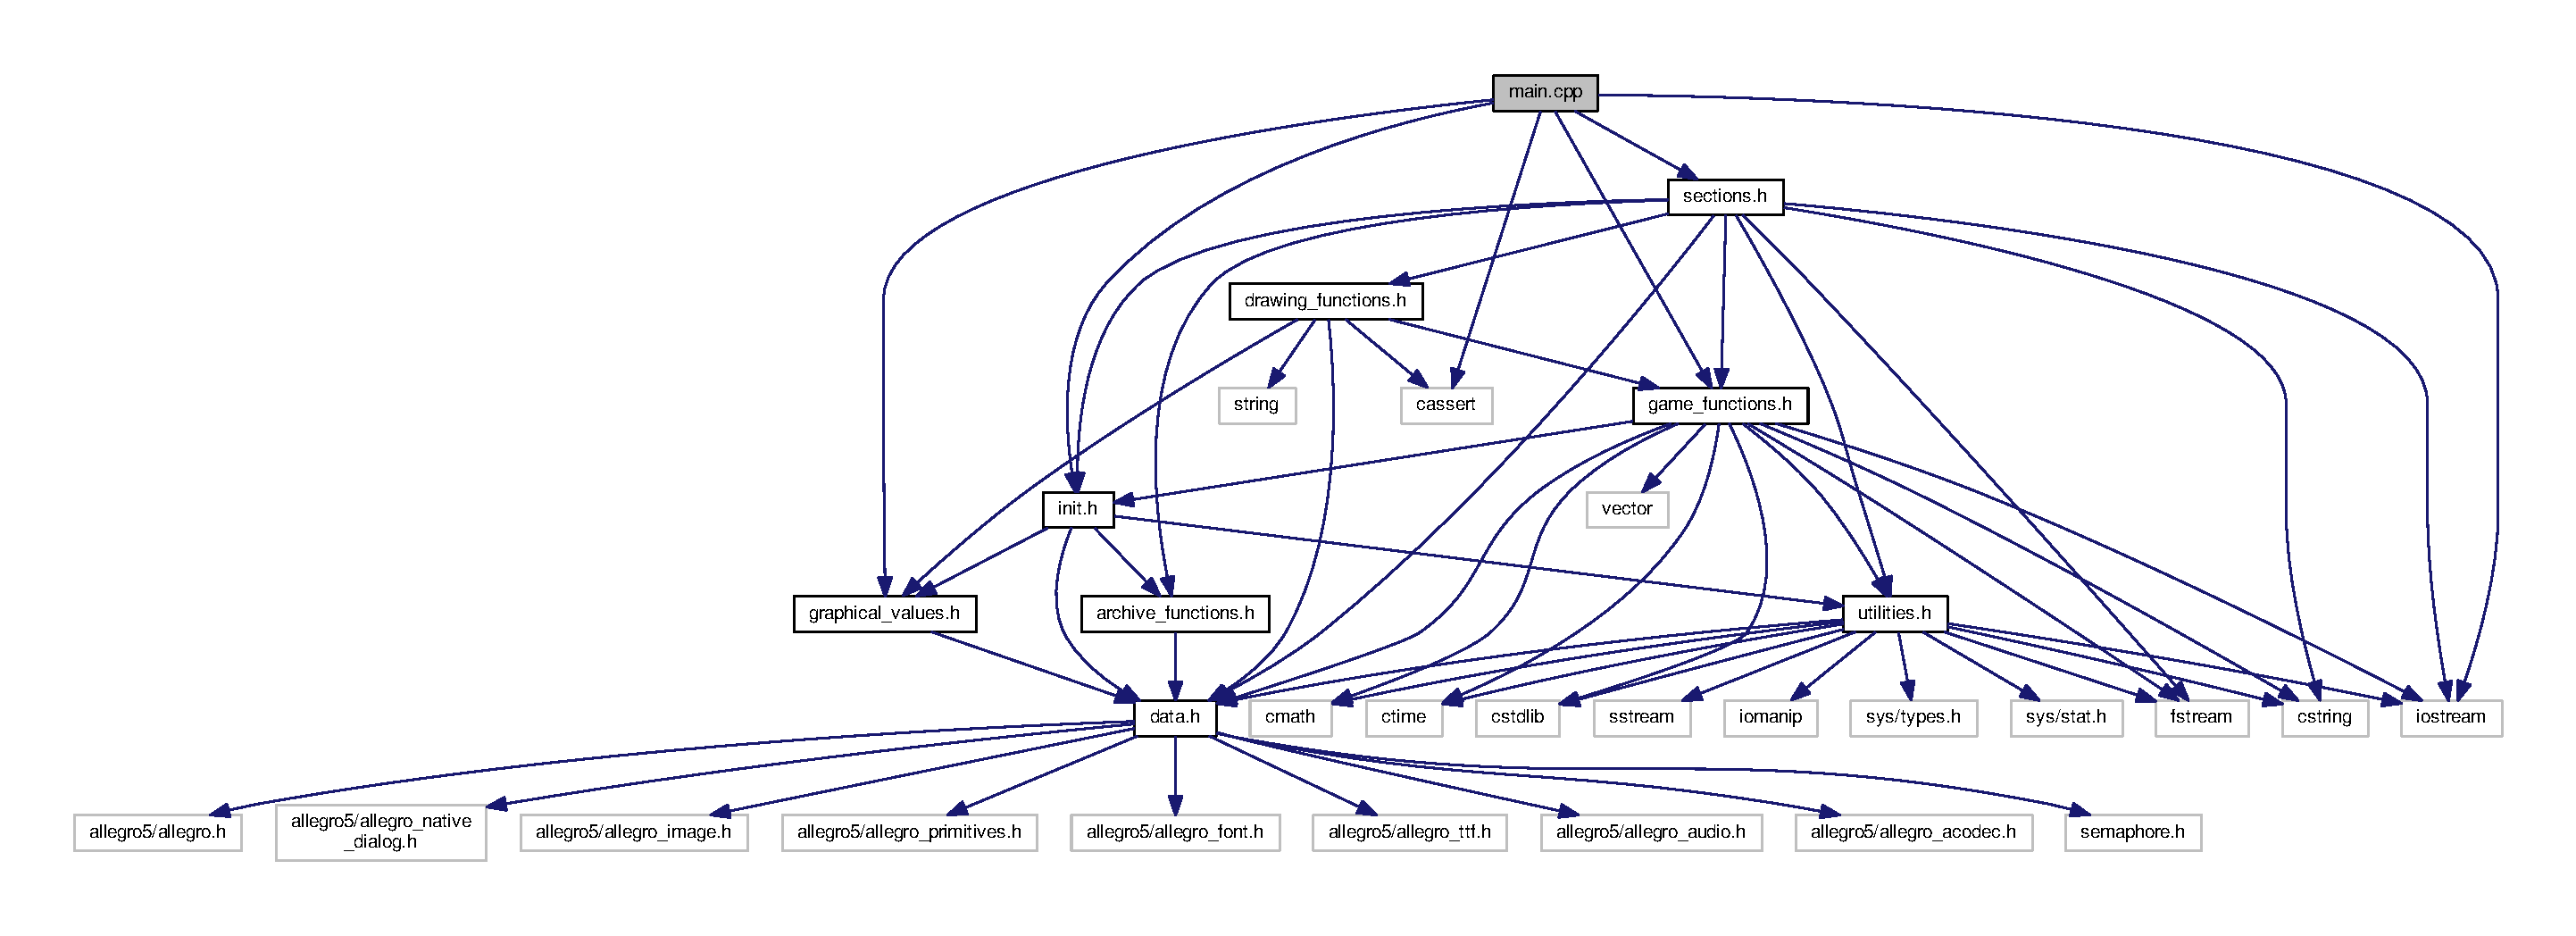
\includegraphics[width=350pt]{da/dce/main_8cpp__incl}
\end{center}
\end{figure}
\subsection*{Funzioni}
\begin{DoxyCompactItemize}
\item 
int \hyperlink{main_8cpp_a3c04138a5bfe5d72780bb7e82a18e627}{main} (int argc, char $\ast$$\ast$argv)
\end{DoxyCompactItemize}
\subsection*{Variabili}
\begin{DoxyCompactItemize}
\item 
\hyperlink{structdisplay__info__t}{display\+\_\+info\+\_\+t} \hyperlink{main_8cpp_a781a8df874545e4f5bff5f8a446d1963}{display\+\_\+info}
\item 
A\+L\+L\+E\+G\+R\+O\+\_\+\+S\+A\+M\+P\+LE $\ast$ \hyperlink{main_8cpp_aaf63227dc3c1f6203248971c305a3e11}{music\+\_\+wa} = nullptr
\item 
\hyperlink{structthread__manager__t}{thread\+\_\+manager\+\_\+t} \hyperlink{main_8cpp_ad04f177b84df22adea5536cbae88451b}{thread\+\_\+manager}
\item 
\hyperlink{structwords__buffer__t}{words\+\_\+buffer\+\_\+t} \hyperlink{main_8cpp_aaa25f9883d8c134861353b1bf5e00846}{words\+\_\+buffer}
\end{DoxyCompactItemize}


\subsection{Documentazione delle funzioni}
\mbox{\Hypertarget{main_8cpp_a3c04138a5bfe5d72780bb7e82a18e627}\label{main_8cpp_a3c04138a5bfe5d72780bb7e82a18e627}} 
\index{main.\+cpp@{main.\+cpp}!main@{main}}
\index{main@{main}!main.\+cpp@{main.\+cpp}}
\subsubsection{\texorpdfstring{main()}{main()}}
{\footnotesize\ttfamily int main (\begin{DoxyParamCaption}\item[{int}]{argc,  }\item[{char $\ast$$\ast$}]{argv }\end{DoxyParamCaption})}

Inizializzazione dimensioni display, e aggiornamento proporzioni grafiche Inizializzazione della coda degli eventi e delle impostazioni Inizializzione e avvio della musica

\subsection{Documentazione delle variabili}
\mbox{\Hypertarget{main_8cpp_a781a8df874545e4f5bff5f8a446d1963}\label{main_8cpp_a781a8df874545e4f5bff5f8a446d1963}} 
\index{main.\+cpp@{main.\+cpp}!display\+\_\+info@{display\+\_\+info}}
\index{display\+\_\+info@{display\+\_\+info}!main.\+cpp@{main.\+cpp}}
\subsubsection{\texorpdfstring{display\+\_\+info}{display\_info}}
{\footnotesize\ttfamily \hyperlink{structdisplay__info__t}{display\+\_\+info\+\_\+t} display\+\_\+info}

\mbox{\Hypertarget{main_8cpp_aaf63227dc3c1f6203248971c305a3e11}\label{main_8cpp_aaf63227dc3c1f6203248971c305a3e11}} 
\index{main.\+cpp@{main.\+cpp}!music\+\_\+wa@{music\+\_\+wa}}
\index{music\+\_\+wa@{music\+\_\+wa}!main.\+cpp@{main.\+cpp}}
\subsubsection{\texorpdfstring{music\+\_\+wa}{music\_wa}}
{\footnotesize\ttfamily A\+L\+L\+E\+G\+R\+O\+\_\+\+S\+A\+M\+P\+LE$\ast$ music\+\_\+wa = nullptr}

\mbox{\Hypertarget{main_8cpp_ad04f177b84df22adea5536cbae88451b}\label{main_8cpp_ad04f177b84df22adea5536cbae88451b}} 
\index{main.\+cpp@{main.\+cpp}!thread\+\_\+manager@{thread\+\_\+manager}}
\index{thread\+\_\+manager@{thread\+\_\+manager}!main.\+cpp@{main.\+cpp}}
\subsubsection{\texorpdfstring{thread\+\_\+manager}{thread\_manager}}
{\footnotesize\ttfamily \hyperlink{structthread__manager__t}{thread\+\_\+manager\+\_\+t} thread\+\_\+manager}

\mbox{\Hypertarget{main_8cpp_aaa25f9883d8c134861353b1bf5e00846}\label{main_8cpp_aaa25f9883d8c134861353b1bf5e00846}} 
\index{main.\+cpp@{main.\+cpp}!words\+\_\+buffer@{words\+\_\+buffer}}
\index{words\+\_\+buffer@{words\+\_\+buffer}!main.\+cpp@{main.\+cpp}}
\subsubsection{\texorpdfstring{words\+\_\+buffer}{words\_buffer}}
{\footnotesize\ttfamily \hyperlink{structwords__buffer__t}{words\+\_\+buffer\+\_\+t} words\+\_\+buffer}


\hypertarget{sections_8cpp}{}\section{Riferimenti per il file sections.\+cpp}
\label{sections_8cpp}\index{sections.\+cpp@{sections.\+cpp}}
{\ttfamily \#include $<$semaphore.\+h$>$}\newline
{\ttfamily \#include \char`\"{}sections.\+h\char`\"{}}\newline
Grafo delle dipendenze di inclusione per sections.\+cpp\+:\nopagebreak
\begin{figure}[H]
\begin{center}
\leavevmode
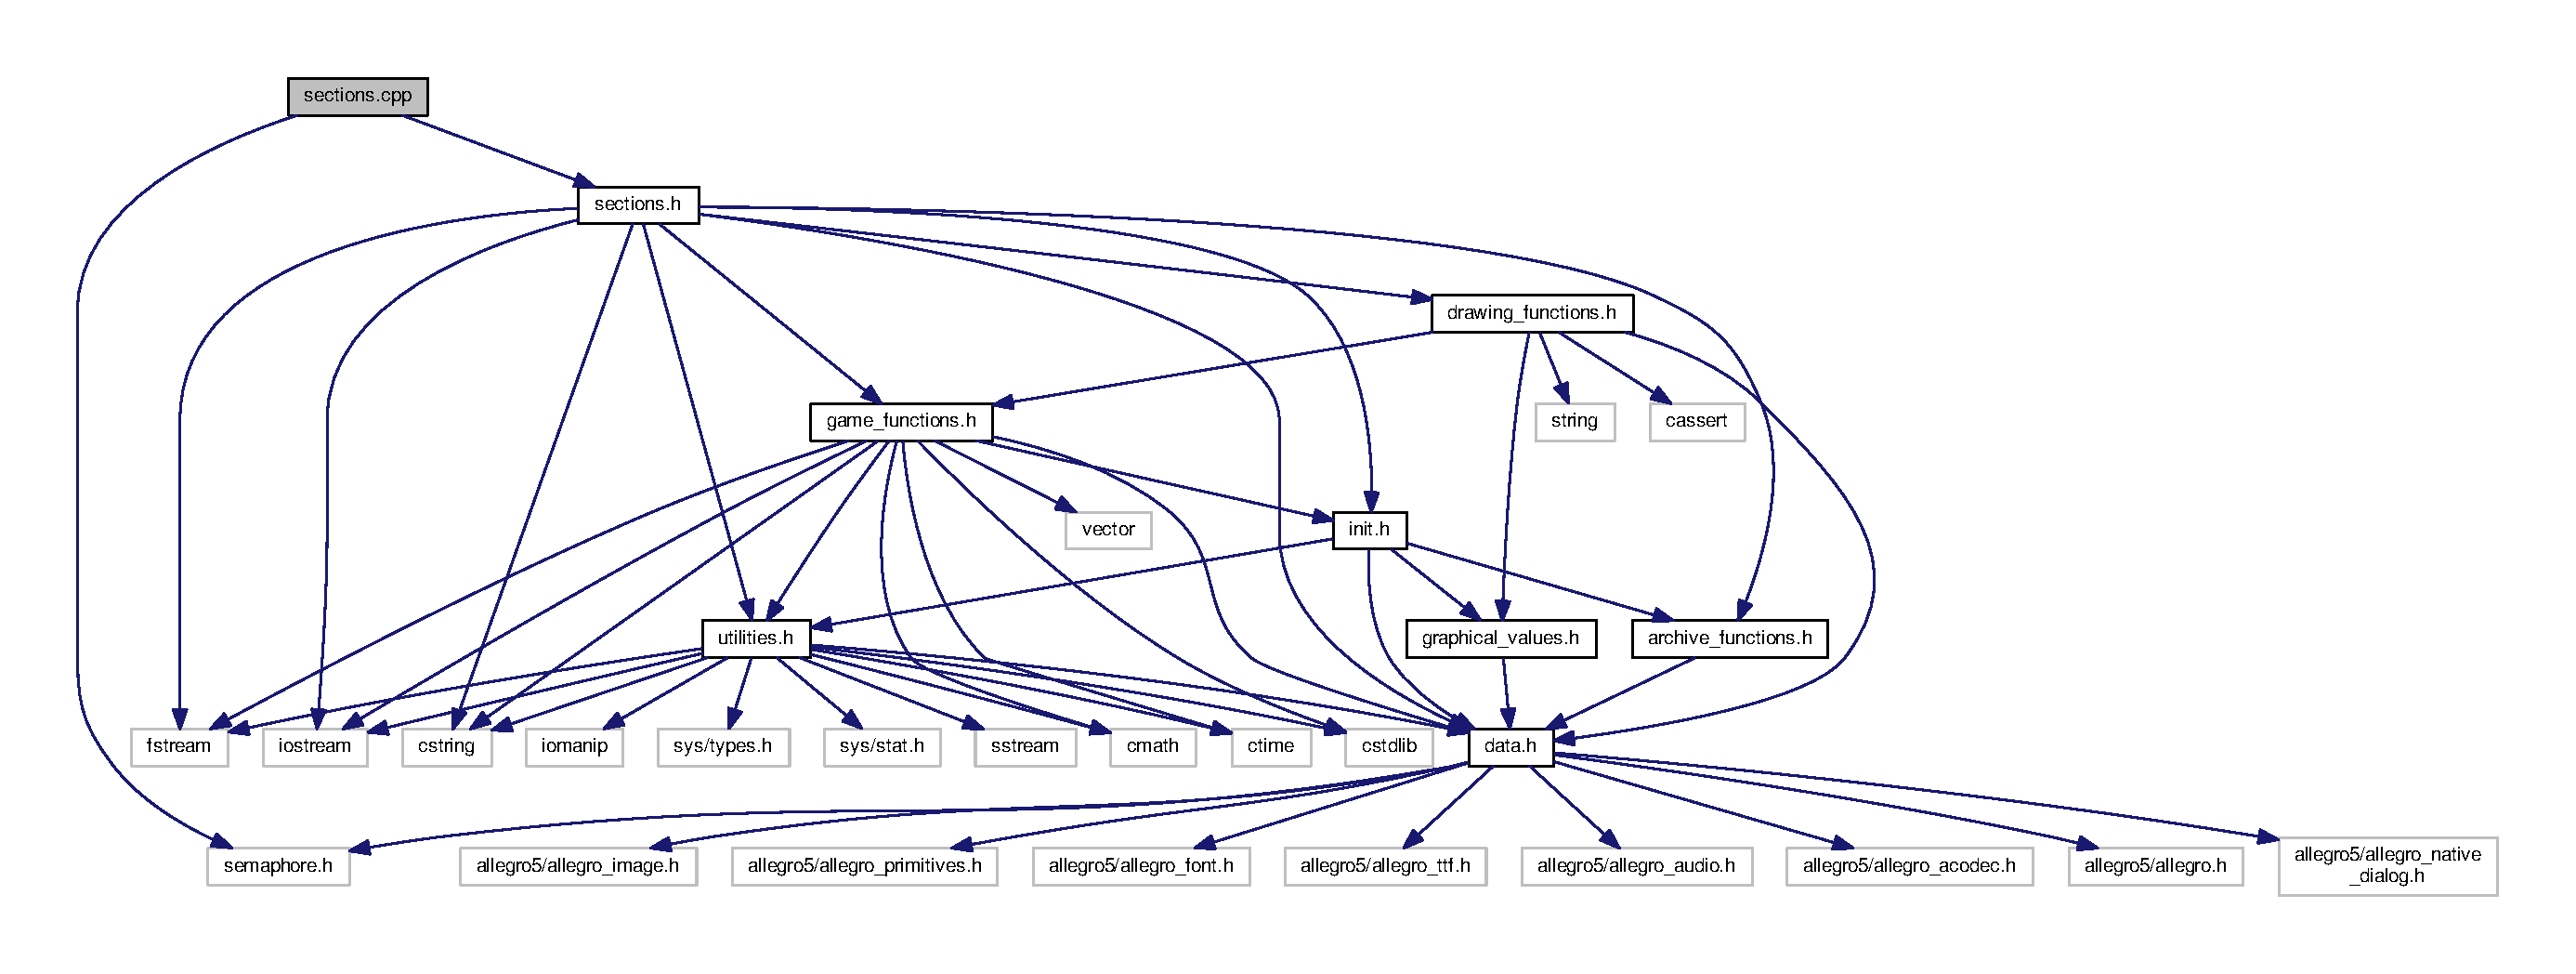
\includegraphics[width=350pt]{d9/d97/sections_8cpp__incl}
\end{center}
\end{figure}
\subsection*{Funzioni}
\begin{DoxyCompactItemize}
\item 
float \hyperlink{sections_8cpp_af70f3c978475d7a7271b784f838ff98b}{intro} (A\+L\+L\+E\+G\+R\+O\+\_\+\+D\+I\+S\+P\+L\+AY $\ast$display)
\begin{DoxyCompactList}\small\item\em Funzione che lancia l\textquotesingle{}animazione di introduzione. \end{DoxyCompactList}\item 
int \hyperlink{sections_8cpp_a57ef27fbb5dfc9331234f3e4769f78bb}{main\+\_\+menu} (A\+L\+L\+E\+G\+R\+O\+\_\+\+D\+I\+S\+P\+L\+AY $\ast$display, A\+L\+L\+E\+G\+R\+O\+\_\+\+E\+V\+E\+N\+T\+\_\+\+Q\+U\+E\+UE $\ast$ev\+\_\+queue, const float \&prev\+\_\+bg\+\_\+offset)
\begin{DoxyCompactList}\small\item\em Funzione che gestisce la schermata del menu principale. \end{DoxyCompactList}\item 
bool \hyperlink{sections_8cpp_a46f019b736168bdc12825c9629e18828}{settings\+\_\+menu} (A\+L\+L\+E\+G\+R\+O\+\_\+\+D\+I\+S\+P\+L\+AY $\ast$display, A\+L\+L\+E\+G\+R\+O\+\_\+\+E\+V\+E\+N\+T\+\_\+\+Q\+U\+E\+UE $\ast$ev\+\_\+queue, \hyperlink{structsettings__t}{settings\+\_\+t} \&settings)
\begin{DoxyCompactList}\small\item\em Funzione che gestisce la schermata del menu delle impostazioni. \end{DoxyCompactList}\item 
bool \hyperlink{sections_8cpp_a77020eac2eeede2d2f733f19cdc9594c}{play\+\_\+wa} (A\+L\+L\+E\+G\+R\+O\+\_\+\+D\+I\+S\+P\+L\+AY $\ast$display, A\+L\+L\+E\+G\+R\+O\+\_\+\+E\+V\+E\+N\+T\+\_\+\+Q\+U\+E\+UE $\ast$ev\+\_\+queue, \hyperlink{structsettings__t}{settings\+\_\+t} \&settings)
\begin{DoxyCompactList}\small\item\em Funzione che gestisce la schermata di gioco. \end{DoxyCompactList}\end{DoxyCompactItemize}


\subsection{Documentazione delle funzioni}
\mbox{\Hypertarget{sections_8cpp_af70f3c978475d7a7271b784f838ff98b}\label{sections_8cpp_af70f3c978475d7a7271b784f838ff98b}} 
\index{sections.\+cpp@{sections.\+cpp}!intro@{intro}}
\index{intro@{intro}!sections.\+cpp@{sections.\+cpp}}
\subsubsection{\texorpdfstring{intro()}{intro()}}
{\footnotesize\ttfamily float intro (\begin{DoxyParamCaption}\item[{A\+L\+L\+E\+G\+R\+O\+\_\+\+D\+I\+S\+P\+L\+AY $\ast$}]{display }\end{DoxyParamCaption})}



Funzione che lancia l\textquotesingle{}animazione di introduzione. 

~\newline
Parametri\+: ~\newline
1) display -\/ Display corrente. ~\newline
Ritorna la posizione dello sfondo a fine funzione (espressa in pixel). \mbox{\Hypertarget{sections_8cpp_a57ef27fbb5dfc9331234f3e4769f78bb}\label{sections_8cpp_a57ef27fbb5dfc9331234f3e4769f78bb}} 
\index{sections.\+cpp@{sections.\+cpp}!main\+\_\+menu@{main\+\_\+menu}}
\index{main\+\_\+menu@{main\+\_\+menu}!sections.\+cpp@{sections.\+cpp}}
\subsubsection{\texorpdfstring{main\+\_\+menu()}{main\_menu()}}
{\footnotesize\ttfamily int main\+\_\+menu (\begin{DoxyParamCaption}\item[{A\+L\+L\+E\+G\+R\+O\+\_\+\+D\+I\+S\+P\+L\+AY $\ast$}]{display,  }\item[{A\+L\+L\+E\+G\+R\+O\+\_\+\+E\+V\+E\+N\+T\+\_\+\+Q\+U\+E\+UE $\ast$}]{ev\+\_\+queue,  }\item[{const float \&}]{prev\+\_\+bg\+\_\+offset }\end{DoxyParamCaption})}



Funzione che gestisce la schermata del menu principale. 

~\newline
Parametri\+: ~\newline
1) display -\/ Display corrente; ~\newline
2) ev\+\_\+queue -\/ Coda degli eventi; ~\newline
3) prev\+\_\+bg\+\_\+offset -\/ Posizione dello sfondo al momento del lancio della funzione. ~\newline
Ritorna la scelta effettuata dall\textquotesingle{}utente. \mbox{\Hypertarget{sections_8cpp_a77020eac2eeede2d2f733f19cdc9594c}\label{sections_8cpp_a77020eac2eeede2d2f733f19cdc9594c}} 
\index{sections.\+cpp@{sections.\+cpp}!play\+\_\+wa@{play\+\_\+wa}}
\index{play\+\_\+wa@{play\+\_\+wa}!sections.\+cpp@{sections.\+cpp}}
\subsubsection{\texorpdfstring{play\+\_\+wa()}{play\_wa()}}
{\footnotesize\ttfamily bool play\+\_\+wa (\begin{DoxyParamCaption}\item[{A\+L\+L\+E\+G\+R\+O\+\_\+\+D\+I\+S\+P\+L\+AY $\ast$}]{display,  }\item[{A\+L\+L\+E\+G\+R\+O\+\_\+\+E\+V\+E\+N\+T\+\_\+\+Q\+U\+E\+UE $\ast$}]{ev\+\_\+queue,  }\item[{\hyperlink{structsettings__t}{settings\+\_\+t} \&}]{settings }\end{DoxyParamCaption})}



Funzione che gestisce la schermata di gioco. 

~\newline
Parametri\+: ~\newline
1) display -\/ Display corrente; ~\newline
2) ev\+\_\+queue -\/ Coda degli eventi; ~\newline
3) settings -\/ Struct contenente le impostazioni di gioco. ~\newline
Ritorna true se la partita termina normalmente, false se l\textquotesingle{}utente decide di uscire dal gioco. \mbox{\Hypertarget{sections_8cpp_a46f019b736168bdc12825c9629e18828}\label{sections_8cpp_a46f019b736168bdc12825c9629e18828}} 
\index{sections.\+cpp@{sections.\+cpp}!settings\+\_\+menu@{settings\+\_\+menu}}
\index{settings\+\_\+menu@{settings\+\_\+menu}!sections.\+cpp@{sections.\+cpp}}
\subsubsection{\texorpdfstring{settings\+\_\+menu()}{settings\_menu()}}
{\footnotesize\ttfamily bool settings\+\_\+menu (\begin{DoxyParamCaption}\item[{A\+L\+L\+E\+G\+R\+O\+\_\+\+D\+I\+S\+P\+L\+AY $\ast$}]{display,  }\item[{A\+L\+L\+E\+G\+R\+O\+\_\+\+E\+V\+E\+N\+T\+\_\+\+Q\+U\+E\+UE $\ast$}]{ev\+\_\+queue,  }\item[{\hyperlink{structsettings__t}{settings\+\_\+t} \&}]{settings }\end{DoxyParamCaption})}



Funzione che gestisce la schermata del menu delle impostazioni. 

~\newline
Parametri\+: ~\newline
1) display -\/ Display corrente; ~\newline
2) ev\+\_\+queue -\/ Coda degli eventi; ~\newline
3) settings -\/ Struct contenente le impostazioni di gioco. ~\newline
Ritorna true se l\textquotesingle{}utente decide di tornare al menu principale, false se decide di uscire dal gioco. 
\hypertarget{sections_8h}{}\section{Riferimenti per il file sections.\+h}
\label{sections_8h}\index{sections.\+h@{sections.\+h}}
{\ttfamily \#include \char`\"{}data.\+h\char`\"{}}\newline
{\ttfamily \#include \char`\"{}init.\+h\char`\"{}}\newline
{\ttfamily \#include \char`\"{}utilities.\+h\char`\"{}}\newline
{\ttfamily \#include \char`\"{}game\+\_\+functions.\+h\char`\"{}}\newline
{\ttfamily \#include \char`\"{}drawing\+\_\+functions.\+h\char`\"{}}\newline
{\ttfamily \#include \char`\"{}archive\+\_\+functions.\+h\char`\"{}}\newline
{\ttfamily \#include $<$cstring$>$}\newline
{\ttfamily \#include $<$iostream$>$}\newline
{\ttfamily \#include $<$fstream$>$}\newline
Grafo delle dipendenze di inclusione per sections.\+h\+:\nopagebreak
\begin{figure}[H]
\begin{center}
\leavevmode
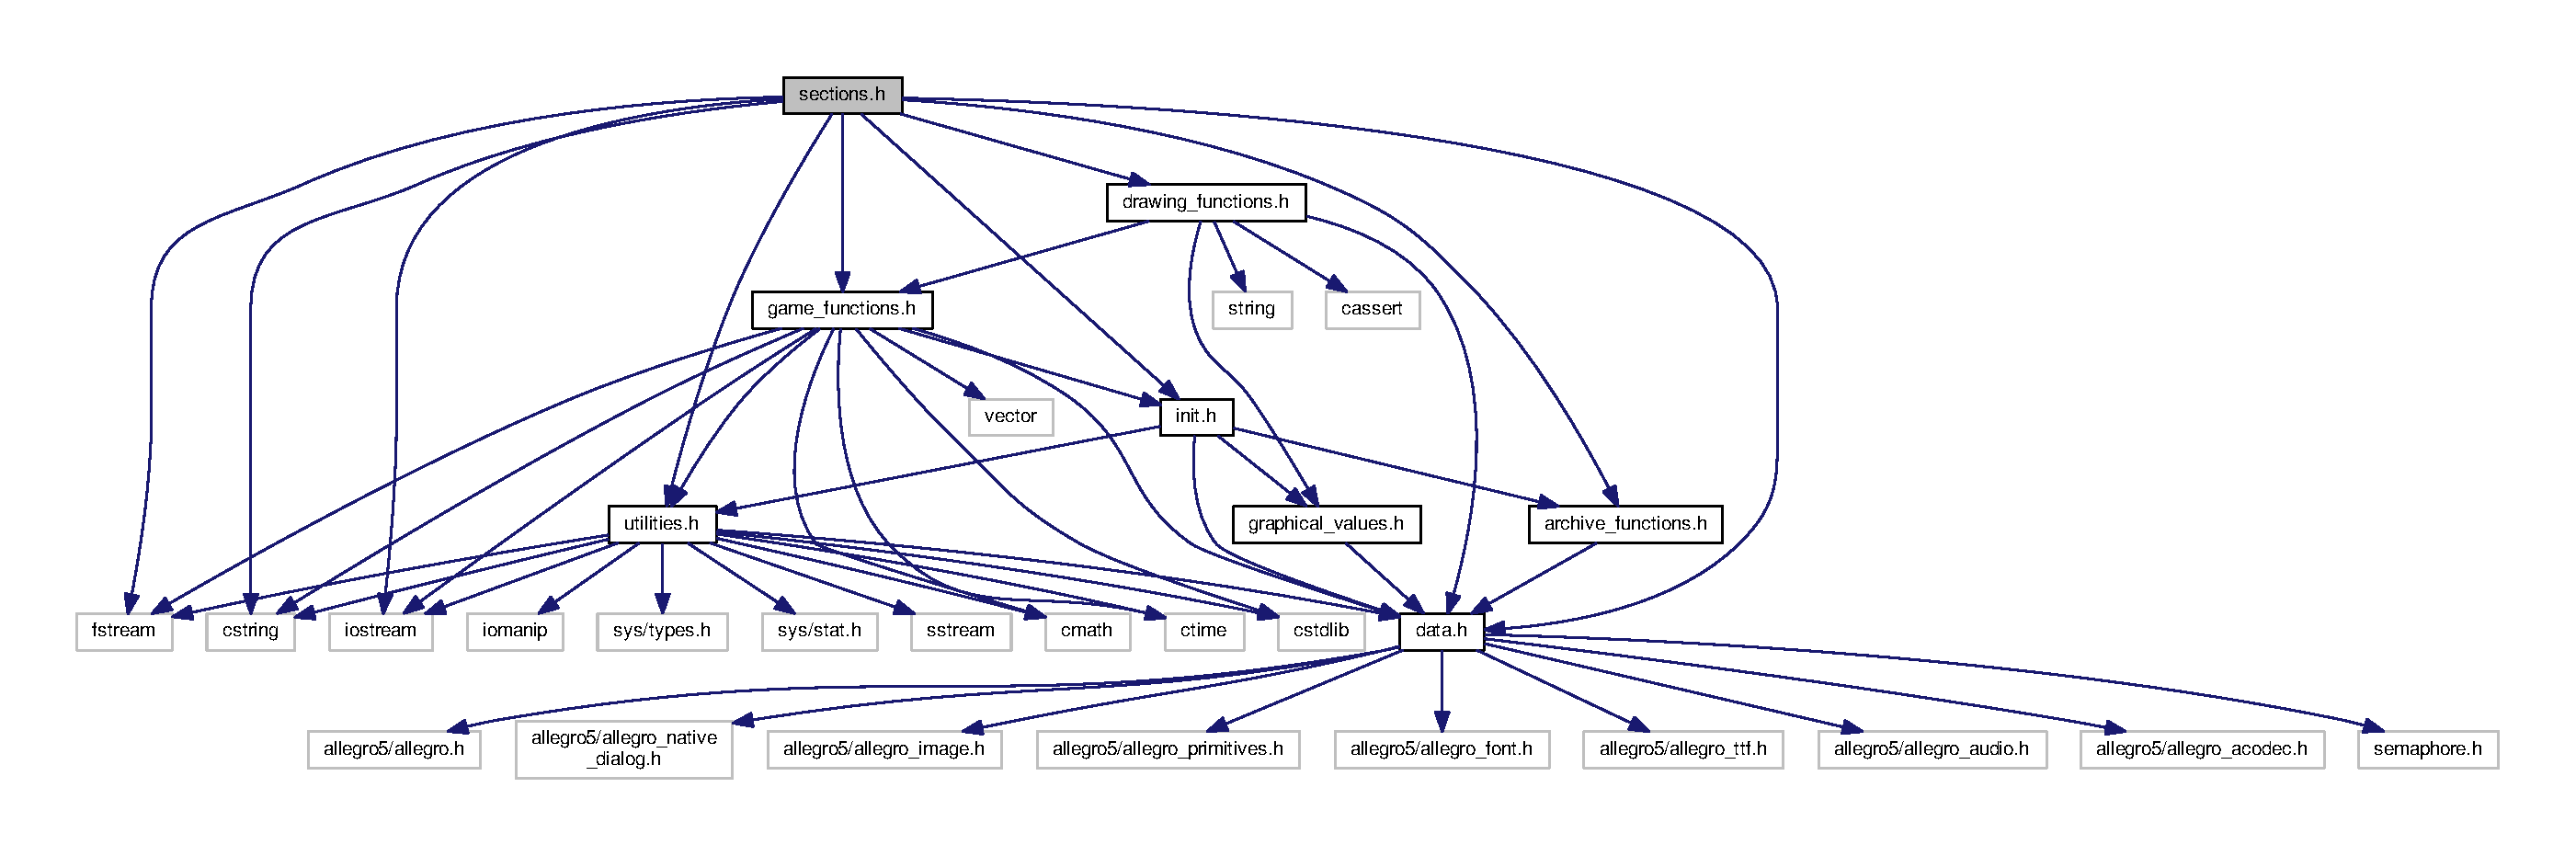
\includegraphics[width=350pt]{d6/d5f/sections_8h__incl}
\end{center}
\end{figure}
Questo grafo mostra quali altri file includono direttamente o indirettamente questo file\+:\nopagebreak
\begin{figure}[H]
\begin{center}
\leavevmode
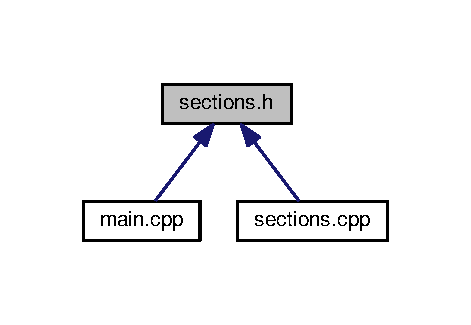
\includegraphics[width=226pt]{dd/d0b/sections_8h__dep__incl}
\end{center}
\end{figure}
\subsection*{Funzioni}
\begin{DoxyCompactItemize}
\item 
float \hyperlink{sections_8h_af70f3c978475d7a7271b784f838ff98b}{intro} (A\+L\+L\+E\+G\+R\+O\+\_\+\+D\+I\+S\+P\+L\+AY $\ast$display)
\begin{DoxyCompactList}\small\item\em Funzione che lancia l\textquotesingle{}animazione di introduzione. \end{DoxyCompactList}\item 
int \hyperlink{sections_8h_a57ef27fbb5dfc9331234f3e4769f78bb}{main\+\_\+menu} (A\+L\+L\+E\+G\+R\+O\+\_\+\+D\+I\+S\+P\+L\+AY $\ast$display, A\+L\+L\+E\+G\+R\+O\+\_\+\+E\+V\+E\+N\+T\+\_\+\+Q\+U\+E\+UE $\ast$ev\+\_\+queue, const float \&prev\+\_\+bg\+\_\+offset)
\begin{DoxyCompactList}\small\item\em Funzione che gestisce la schermata del menu principale. \end{DoxyCompactList}\item 
bool \hyperlink{sections_8h_a46f019b736168bdc12825c9629e18828}{settings\+\_\+menu} (A\+L\+L\+E\+G\+R\+O\+\_\+\+D\+I\+S\+P\+L\+AY $\ast$display, A\+L\+L\+E\+G\+R\+O\+\_\+\+E\+V\+E\+N\+T\+\_\+\+Q\+U\+E\+UE $\ast$ev\+\_\+queue, \hyperlink{structsettings__t}{settings\+\_\+t} \&settings)
\begin{DoxyCompactList}\small\item\em Funzione che gestisce la schermata del menu delle impostazioni. \end{DoxyCompactList}\item 
bool \hyperlink{sections_8h_a77020eac2eeede2d2f733f19cdc9594c}{play\+\_\+wa} (A\+L\+L\+E\+G\+R\+O\+\_\+\+D\+I\+S\+P\+L\+AY $\ast$display, A\+L\+L\+E\+G\+R\+O\+\_\+\+E\+V\+E\+N\+T\+\_\+\+Q\+U\+E\+UE $\ast$ev\+\_\+queue, \hyperlink{structsettings__t}{settings\+\_\+t} \&settings)
\begin{DoxyCompactList}\small\item\em Funzione che gestisce la schermata di gioco. \end{DoxyCompactList}\end{DoxyCompactItemize}
\subsection*{Variabili}
\begin{DoxyCompactItemize}
\item 
\hyperlink{structdisplay__info__t}{display\+\_\+info\+\_\+t} \hyperlink{sections_8h_a781a8df874545e4f5bff5f8a446d1963}{display\+\_\+info}
\item 
\hyperlink{structthread__manager__t}{thread\+\_\+manager\+\_\+t} \hyperlink{sections_8h_ad04f177b84df22adea5536cbae88451b}{thread\+\_\+manager}
\item 
\hyperlink{structwords__buffer__t}{words\+\_\+buffer\+\_\+t} \hyperlink{sections_8h_aaa25f9883d8c134861353b1bf5e00846}{words\+\_\+buffer}
\item 
\hyperlink{structmenu__gv__t}{menu\+\_\+gv\+\_\+t} \hyperlink{sections_8h_a8050b794d70ca38807298569dc1af9b1}{M\+E\+N\+U\+\_\+\+GV}
\begin{DoxyCompactList}\small\item\em Struct contenente le proporzioni grafiche dei menu. \end{DoxyCompactList}\item 
\hyperlink{structusr__gv__t}{usr\+\_\+gv\+\_\+t} \hyperlink{sections_8h_aba4a0deff6c9de510c6621913ab2a406}{U\+S\+R\+\_\+\+GV}
\begin{DoxyCompactList}\small\item\em Struct contenente le proporzioni grafiche della schermata di fine partita. \end{DoxyCompactList}\item 
A\+L\+L\+E\+G\+R\+O\+\_\+\+S\+A\+M\+P\+LE $\ast$ \hyperlink{sections_8h_aaf63227dc3c1f6203248971c305a3e11}{music\+\_\+wa}
\end{DoxyCompactItemize}


\subsection{Documentazione delle funzioni}
\mbox{\Hypertarget{sections_8h_af70f3c978475d7a7271b784f838ff98b}\label{sections_8h_af70f3c978475d7a7271b784f838ff98b}} 
\index{sections.\+h@{sections.\+h}!intro@{intro}}
\index{intro@{intro}!sections.\+h@{sections.\+h}}
\subsubsection{\texorpdfstring{intro()}{intro()}}
{\footnotesize\ttfamily float intro (\begin{DoxyParamCaption}\item[{A\+L\+L\+E\+G\+R\+O\+\_\+\+D\+I\+S\+P\+L\+AY $\ast$}]{display }\end{DoxyParamCaption})}



Funzione che lancia l\textquotesingle{}animazione di introduzione. 

~\newline
Parametri\+: ~\newline
1) display -\/ Display corrente. ~\newline
Ritorna la posizione dello sfondo a fine funzione (espressa in pixel). \mbox{\Hypertarget{sections_8h_a57ef27fbb5dfc9331234f3e4769f78bb}\label{sections_8h_a57ef27fbb5dfc9331234f3e4769f78bb}} 
\index{sections.\+h@{sections.\+h}!main\+\_\+menu@{main\+\_\+menu}}
\index{main\+\_\+menu@{main\+\_\+menu}!sections.\+h@{sections.\+h}}
\subsubsection{\texorpdfstring{main\+\_\+menu()}{main\_menu()}}
{\footnotesize\ttfamily int main\+\_\+menu (\begin{DoxyParamCaption}\item[{A\+L\+L\+E\+G\+R\+O\+\_\+\+D\+I\+S\+P\+L\+AY $\ast$}]{display,  }\item[{A\+L\+L\+E\+G\+R\+O\+\_\+\+E\+V\+E\+N\+T\+\_\+\+Q\+U\+E\+UE $\ast$}]{ev\+\_\+queue,  }\item[{const float \&}]{prev\+\_\+bg\+\_\+offset }\end{DoxyParamCaption})}



Funzione che gestisce la schermata del menu principale. 

~\newline
Parametri\+: ~\newline
1) display -\/ Display corrente; ~\newline
2) ev\+\_\+queue -\/ Coda degli eventi; ~\newline
3) prev\+\_\+bg\+\_\+offset -\/ Posizione dello sfondo al momento del lancio della funzione. ~\newline
Ritorna la scelta effettuata dall\textquotesingle{}utente. \mbox{\Hypertarget{sections_8h_a77020eac2eeede2d2f733f19cdc9594c}\label{sections_8h_a77020eac2eeede2d2f733f19cdc9594c}} 
\index{sections.\+h@{sections.\+h}!play\+\_\+wa@{play\+\_\+wa}}
\index{play\+\_\+wa@{play\+\_\+wa}!sections.\+h@{sections.\+h}}
\subsubsection{\texorpdfstring{play\+\_\+wa()}{play\_wa()}}
{\footnotesize\ttfamily bool play\+\_\+wa (\begin{DoxyParamCaption}\item[{A\+L\+L\+E\+G\+R\+O\+\_\+\+D\+I\+S\+P\+L\+AY $\ast$}]{display,  }\item[{A\+L\+L\+E\+G\+R\+O\+\_\+\+E\+V\+E\+N\+T\+\_\+\+Q\+U\+E\+UE $\ast$}]{ev\+\_\+queue,  }\item[{\hyperlink{structsettings__t}{settings\+\_\+t} \&}]{settings }\end{DoxyParamCaption})}



Funzione che gestisce la schermata di gioco. 

~\newline
Parametri\+: ~\newline
1) display -\/ Display corrente; ~\newline
2) ev\+\_\+queue -\/ Coda degli eventi; ~\newline
3) settings -\/ Struct contenente le impostazioni di gioco. ~\newline
Ritorna true se la partita termina normalmente, false se l\textquotesingle{}utente decide di uscire dal gioco. \mbox{\Hypertarget{sections_8h_a46f019b736168bdc12825c9629e18828}\label{sections_8h_a46f019b736168bdc12825c9629e18828}} 
\index{sections.\+h@{sections.\+h}!settings\+\_\+menu@{settings\+\_\+menu}}
\index{settings\+\_\+menu@{settings\+\_\+menu}!sections.\+h@{sections.\+h}}
\subsubsection{\texorpdfstring{settings\+\_\+menu()}{settings\_menu()}}
{\footnotesize\ttfamily bool settings\+\_\+menu (\begin{DoxyParamCaption}\item[{A\+L\+L\+E\+G\+R\+O\+\_\+\+D\+I\+S\+P\+L\+AY $\ast$}]{display,  }\item[{A\+L\+L\+E\+G\+R\+O\+\_\+\+E\+V\+E\+N\+T\+\_\+\+Q\+U\+E\+UE $\ast$}]{ev\+\_\+queue,  }\item[{\hyperlink{structsettings__t}{settings\+\_\+t} \&}]{settings }\end{DoxyParamCaption})}



Funzione che gestisce la schermata del menu delle impostazioni. 

~\newline
Parametri\+: ~\newline
1) display -\/ Display corrente; ~\newline
2) ev\+\_\+queue -\/ Coda degli eventi; ~\newline
3) settings -\/ Struct contenente le impostazioni di gioco. ~\newline
Ritorna true se l\textquotesingle{}utente decide di tornare al menu principale, false se decide di uscire dal gioco. 

\subsection{Documentazione delle variabili}
\mbox{\Hypertarget{sections_8h_a781a8df874545e4f5bff5f8a446d1963}\label{sections_8h_a781a8df874545e4f5bff5f8a446d1963}} 
\index{sections.\+h@{sections.\+h}!display\+\_\+info@{display\+\_\+info}}
\index{display\+\_\+info@{display\+\_\+info}!sections.\+h@{sections.\+h}}
\subsubsection{\texorpdfstring{display\+\_\+info}{display\_info}}
{\footnotesize\ttfamily \hyperlink{structdisplay__info__t}{display\+\_\+info\+\_\+t} display\+\_\+info}

\mbox{\Hypertarget{sections_8h_a8050b794d70ca38807298569dc1af9b1}\label{sections_8h_a8050b794d70ca38807298569dc1af9b1}} 
\index{sections.\+h@{sections.\+h}!M\+E\+N\+U\+\_\+\+GV@{M\+E\+N\+U\+\_\+\+GV}}
\index{M\+E\+N\+U\+\_\+\+GV@{M\+E\+N\+U\+\_\+\+GV}!sections.\+h@{sections.\+h}}
\subsubsection{\texorpdfstring{M\+E\+N\+U\+\_\+\+GV}{MENU\_GV}}
{\footnotesize\ttfamily \hyperlink{structmenu__gv__t}{menu\+\_\+gv\+\_\+t} M\+E\+N\+U\+\_\+\+GV}



Struct contenente le proporzioni grafiche dei menu. 

\mbox{\Hypertarget{sections_8h_aaf63227dc3c1f6203248971c305a3e11}\label{sections_8h_aaf63227dc3c1f6203248971c305a3e11}} 
\index{sections.\+h@{sections.\+h}!music\+\_\+wa@{music\+\_\+wa}}
\index{music\+\_\+wa@{music\+\_\+wa}!sections.\+h@{sections.\+h}}
\subsubsection{\texorpdfstring{music\+\_\+wa}{music\_wa}}
{\footnotesize\ttfamily A\+L\+L\+E\+G\+R\+O\+\_\+\+S\+A\+M\+P\+LE$\ast$ music\+\_\+wa}

\mbox{\Hypertarget{sections_8h_ad04f177b84df22adea5536cbae88451b}\label{sections_8h_ad04f177b84df22adea5536cbae88451b}} 
\index{sections.\+h@{sections.\+h}!thread\+\_\+manager@{thread\+\_\+manager}}
\index{thread\+\_\+manager@{thread\+\_\+manager}!sections.\+h@{sections.\+h}}
\subsubsection{\texorpdfstring{thread\+\_\+manager}{thread\_manager}}
{\footnotesize\ttfamily \hyperlink{structthread__manager__t}{thread\+\_\+manager\+\_\+t} thread\+\_\+manager}

\mbox{\Hypertarget{sections_8h_aba4a0deff6c9de510c6621913ab2a406}\label{sections_8h_aba4a0deff6c9de510c6621913ab2a406}} 
\index{sections.\+h@{sections.\+h}!U\+S\+R\+\_\+\+GV@{U\+S\+R\+\_\+\+GV}}
\index{U\+S\+R\+\_\+\+GV@{U\+S\+R\+\_\+\+GV}!sections.\+h@{sections.\+h}}
\subsubsection{\texorpdfstring{U\+S\+R\+\_\+\+GV}{USR\_GV}}
{\footnotesize\ttfamily \hyperlink{structusr__gv__t}{usr\+\_\+gv\+\_\+t} U\+S\+R\+\_\+\+GV}



Struct contenente le proporzioni grafiche della schermata di fine partita. 

\mbox{\Hypertarget{sections_8h_aaa25f9883d8c134861353b1bf5e00846}\label{sections_8h_aaa25f9883d8c134861353b1bf5e00846}} 
\index{sections.\+h@{sections.\+h}!words\+\_\+buffer@{words\+\_\+buffer}}
\index{words\+\_\+buffer@{words\+\_\+buffer}!sections.\+h@{sections.\+h}}
\subsubsection{\texorpdfstring{words\+\_\+buffer}{words\_buffer}}
{\footnotesize\ttfamily \hyperlink{structwords__buffer__t}{words\+\_\+buffer\+\_\+t} words\+\_\+buffer}


\hypertarget{utilities_8cpp}{}\section{Riferimenti per il file utilities.\+cpp}
\label{utilities_8cpp}\index{utilities.\+cpp@{utilities.\+cpp}}
{\ttfamily \#include $<$dirent.\+h$>$}\newline
{\ttfamily \#include \char`\"{}utilities.\+h\char`\"{}}\newline
Grafo delle dipendenze di inclusione per utilities.\+cpp\+:\nopagebreak
\begin{figure}[H]
\begin{center}
\leavevmode
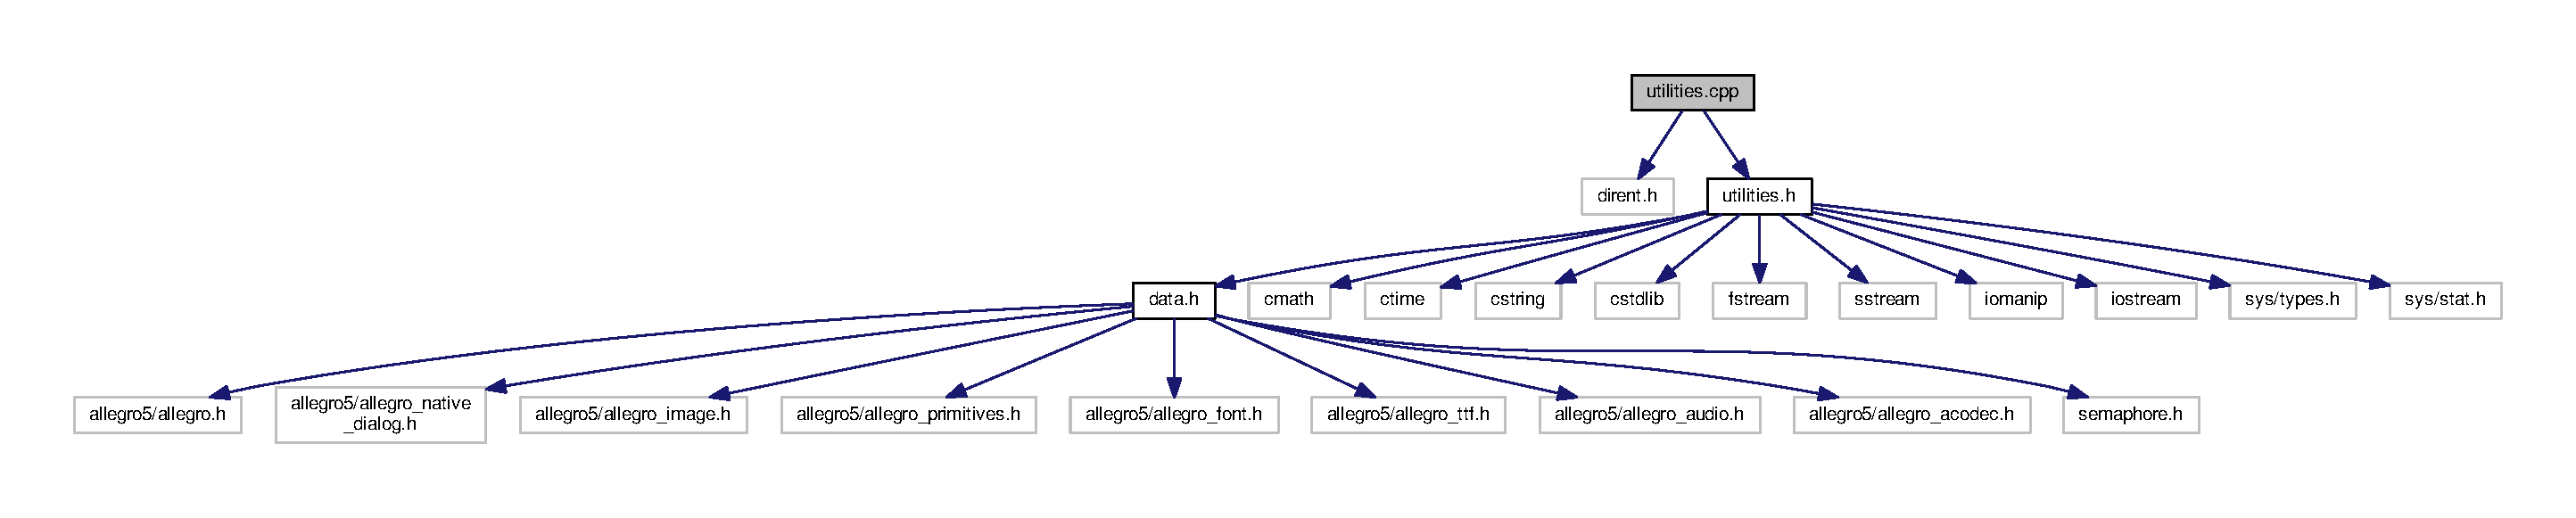
\includegraphics[width=350pt]{df/d5d/utilities_8cpp__incl}
\end{center}
\end{figure}
\subsection*{Funzioni}
\begin{DoxyCompactItemize}
\item 
bool \hyperlink{utilities_8cpp_a08c469e6eee9ca9956ac35d64d2124ef}{exit} (A\+L\+L\+E\+G\+R\+O\+\_\+\+D\+I\+S\+P\+L\+AY $\ast$display, const bool playing)
\begin{DoxyCompactList}\small\item\em Funzione ausiliaria che genera un alert con la richiesta di uscire dal gioco. \end{DoxyCompactList}\item 
char $\ast$ \hyperlink{utilities_8cpp_a09cadb87c7167c969102c415ad70842d}{int\+\_\+to\+\_\+str\+\_\+score} (const int \&match\+\_\+score)
\begin{DoxyCompactList}\small\item\em Funzione che converte il punteggio (intero) in una stringa di otto caratteri. \end{DoxyCompactList}\item 
int \hyperlink{utilities_8cpp_a9ec487f04fb6ccf162c3fc8f0e672780}{which\+\_\+quadrant} (const float x, const float y)
\begin{DoxyCompactList}\small\item\em Funzione che, dato un certo punto del display, restituisce il quadrante (1-\/4) al quale appartiene. \end{DoxyCompactList}\item 
void \hyperlink{utilities_8cpp_aeee1998bab6461ac3281a2fd7522a8b9}{extract\+\_\+elem} (\hyperlink{data_8h_a452eef9acfcf76fb85e2c7ecf3b9ff90}{asteroid\+\_\+list} $\ast$ast\+\_\+queues, const int \&index\+\_\+to\+\_\+extract)
\begin{DoxyCompactList}\small\item\em Funzione che estrai l\textquotesingle{}elemento dalla coda. \end{DoxyCompactList}\item 
int \hyperlink{utilities_8cpp_a045d229cb85f3dbc0d99a421cdcf2a3f}{insert\+\_\+elem\+\_\+head} (\hyperlink{data_8h_a452eef9acfcf76fb85e2c7ecf3b9ff90}{asteroid\+\_\+list} $\ast$ast\+\_\+queues, const \hyperlink{structasteroid__t}{asteroid\+\_\+t} \&asteroid)
\begin{DoxyCompactList}\small\item\em Funzione che inserisce un elemento nella lista, con un controllo se l\textquotesingle{}elemento è inserito in testa o in coda. \end{DoxyCompactList}\item 
void \hyperlink{utilities_8cpp_a5c24fe2f533da0dea022ccdb2ac665bb}{change\+\_\+enable} (\hyperlink{data_8h_a56839c56ca6deb3cff5e21540ddb8218}{enable\+\_\+t} \&enabled)
\begin{DoxyCompactList}\small\item\em Funzione adibita al set/reset di una determinata impostazione di gioco. \end{DoxyCompactList}\item 
void \hyperlink{utilities_8cpp_adcafafb6c87ae3399e1d4889a5d5dcce}{delete\+\_\+ast\+\_\+queues} (\hyperlink{data_8h_a452eef9acfcf76fb85e2c7ecf3b9ff90}{asteroid\+\_\+list} $\ast$ast\+\_\+queues)
\begin{DoxyCompactList}\small\item\em Funzione che dealloca gli asteroidi in gioco a fine partita e le relativi immagini. \end{DoxyCompactList}\item 
void \hyperlink{utilities_8cpp_a68fad52f9f7a53fa048bafc47528a1bb}{delete\+\_\+timer} (\hyperlink{structmatch__vars__t}{match\+\_\+vars\+\_\+t} \&match\+\_\+vars)
\begin{DoxyCompactList}\small\item\em Funzione che dealloca i timer utilizzati come appoggio durante la partita. \end{DoxyCompactList}\item 
void \hyperlink{utilities_8cpp_a1f78e2ccd2b9605cd499c1d5c7fd62ec}{delete\+\_\+display\+\_\+evqueue\+\_\+music} (A\+L\+L\+E\+G\+R\+O\+\_\+\+D\+I\+S\+P\+L\+AY $\ast$display, A\+L\+L\+E\+G\+R\+O\+\_\+\+E\+V\+E\+N\+T\+\_\+\+Q\+U\+E\+UE $\ast$ev\+\_\+queue, A\+L\+L\+E\+G\+R\+O\+\_\+\+S\+A\+M\+P\+LE $\ast$sound)
\begin{DoxyCompactList}\small\item\em Funzione che dealloca il display, la coda degli eventi e la musica alla chiusera del gioco. \end{DoxyCompactList}\item 
void \hyperlink{utilities_8cpp_ab1ffd16a1c007a9d9029fc4eaea4abdb}{delete\+\_\+sounds} (\hyperlink{structmatch__vars__t}{match\+\_\+vars\+\_\+t} \&match\+\_\+vars)
\begin{DoxyCompactList}\small\item\em Funzione che dealloca i suoni durante la singola partita. \end{DoxyCompactList}\item 
bool \hyperlink{utilities_8cpp_a3e3556f55af2c53b4b2790b2e9130b27}{ls\+\_\+tar} (\hyperlink{structls__t}{ls\+\_\+t} $\ast$ls)
\begin{DoxyCompactList}\small\item\em Funzione che restituisce la lista di archivi presenti nella cartella. \end{DoxyCompactList}\item 
bool \hyperlink{utilities_8cpp_aa56ac46388226ecf231b9da96c5d9084}{archives\+\_\+exist} ()
\begin{DoxyCompactList}\small\item\em Funzione true nel caso la cartella indicata durante la compilazione del programma contenga archivi validi. \end{DoxyCompactList}\end{DoxyCompactItemize}


\subsection{Documentazione delle funzioni}
\mbox{\Hypertarget{utilities_8cpp_aa56ac46388226ecf231b9da96c5d9084}\label{utilities_8cpp_aa56ac46388226ecf231b9da96c5d9084}} 
\index{utilities.\+cpp@{utilities.\+cpp}!archives\+\_\+exist@{archives\+\_\+exist}}
\index{archives\+\_\+exist@{archives\+\_\+exist}!utilities.\+cpp@{utilities.\+cpp}}
\subsubsection{\texorpdfstring{archives\+\_\+exist()}{archives\_exist()}}
{\footnotesize\ttfamily bool archives\+\_\+exist (\begin{DoxyParamCaption}{ }\end{DoxyParamCaption})}



Funzione true nel caso la cartella indicata durante la compilazione del programma contenga archivi validi. 

~\newline
Ritorna false altrimenti. \mbox{\Hypertarget{utilities_8cpp_a5c24fe2f533da0dea022ccdb2ac665bb}\label{utilities_8cpp_a5c24fe2f533da0dea022ccdb2ac665bb}} 
\index{utilities.\+cpp@{utilities.\+cpp}!change\+\_\+enable@{change\+\_\+enable}}
\index{change\+\_\+enable@{change\+\_\+enable}!utilities.\+cpp@{utilities.\+cpp}}
\subsubsection{\texorpdfstring{change\+\_\+enable()}{change\_enable()}}
{\footnotesize\ttfamily void change\+\_\+enable (\begin{DoxyParamCaption}\item[{\hyperlink{data_8h_a56839c56ca6deb3cff5e21540ddb8218}{enable\+\_\+t} \&}]{enable }\end{DoxyParamCaption})}



Funzione adibita al set/reset di una determinata impostazione di gioco. 

~\newline
Parametri\+: ~\newline
1) enable -\/ Impostazione corrente. \mbox{\Hypertarget{utilities_8cpp_adcafafb6c87ae3399e1d4889a5d5dcce}\label{utilities_8cpp_adcafafb6c87ae3399e1d4889a5d5dcce}} 
\index{utilities.\+cpp@{utilities.\+cpp}!delete\+\_\+ast\+\_\+queues@{delete\+\_\+ast\+\_\+queues}}
\index{delete\+\_\+ast\+\_\+queues@{delete\+\_\+ast\+\_\+queues}!utilities.\+cpp@{utilities.\+cpp}}
\subsubsection{\texorpdfstring{delete\+\_\+ast\+\_\+queues()}{delete\_ast\_queues()}}
{\footnotesize\ttfamily void delete\+\_\+ast\+\_\+queues (\begin{DoxyParamCaption}\item[{\hyperlink{data_8h_a452eef9acfcf76fb85e2c7ecf3b9ff90}{asteroid\+\_\+list} $\ast$}]{ast\+\_\+queues }\end{DoxyParamCaption})}



Funzione che dealloca gli asteroidi in gioco a fine partita e le relativi immagini. 

~\newline
Parametri\+: ~\newline
1) ast\+\_\+queues -\/ Vettore di liste di asteroidi. \mbox{\Hypertarget{utilities_8cpp_a1f78e2ccd2b9605cd499c1d5c7fd62ec}\label{utilities_8cpp_a1f78e2ccd2b9605cd499c1d5c7fd62ec}} 
\index{utilities.\+cpp@{utilities.\+cpp}!delete\+\_\+display\+\_\+evqueue\+\_\+music@{delete\+\_\+display\+\_\+evqueue\+\_\+music}}
\index{delete\+\_\+display\+\_\+evqueue\+\_\+music@{delete\+\_\+display\+\_\+evqueue\+\_\+music}!utilities.\+cpp@{utilities.\+cpp}}
\subsubsection{\texorpdfstring{delete\+\_\+display\+\_\+evqueue\+\_\+music()}{delete\_display\_evqueue\_music()}}
{\footnotesize\ttfamily void delete\+\_\+display\+\_\+evqueue\+\_\+music (\begin{DoxyParamCaption}\item[{A\+L\+L\+E\+G\+R\+O\+\_\+\+D\+I\+S\+P\+L\+AY $\ast$}]{display,  }\item[{A\+L\+L\+E\+G\+R\+O\+\_\+\+E\+V\+E\+N\+T\+\_\+\+Q\+U\+E\+UE $\ast$}]{ev\+\_\+queue,  }\item[{A\+L\+L\+E\+G\+R\+O\+\_\+\+S\+A\+M\+P\+LE $\ast$}]{sound }\end{DoxyParamCaption})}



Funzione che dealloca il display, la coda degli eventi e la musica alla chiusera del gioco. 

Parametri\+: ~\newline
1) display -\/ Puntatore al display del gioco; ~\newline
2) ev\+\_\+queue -\/ Puntatore alla coda di eventi; ~\newline
3) sound -\/ Puntatore alla musica del gioco. \mbox{\Hypertarget{utilities_8cpp_ab1ffd16a1c007a9d9029fc4eaea4abdb}\label{utilities_8cpp_ab1ffd16a1c007a9d9029fc4eaea4abdb}} 
\index{utilities.\+cpp@{utilities.\+cpp}!delete\+\_\+sounds@{delete\+\_\+sounds}}
\index{delete\+\_\+sounds@{delete\+\_\+sounds}!utilities.\+cpp@{utilities.\+cpp}}
\subsubsection{\texorpdfstring{delete\+\_\+sounds()}{delete\_sounds()}}
{\footnotesize\ttfamily void delete\+\_\+sounds (\begin{DoxyParamCaption}\item[{\hyperlink{structmatch__vars__t}{match\+\_\+vars\+\_\+t} \&}]{match\+\_\+vars }\end{DoxyParamCaption})}



Funzione che dealloca i suoni durante la singola partita. 

~\newline
Parametri\+: ~\newline
1) match\+\_\+vars -\/ Contenitore dei puntatori agli audio. \mbox{\Hypertarget{utilities_8cpp_a68fad52f9f7a53fa048bafc47528a1bb}\label{utilities_8cpp_a68fad52f9f7a53fa048bafc47528a1bb}} 
\index{utilities.\+cpp@{utilities.\+cpp}!delete\+\_\+timer@{delete\+\_\+timer}}
\index{delete\+\_\+timer@{delete\+\_\+timer}!utilities.\+cpp@{utilities.\+cpp}}
\subsubsection{\texorpdfstring{delete\+\_\+timer()}{delete\_timer()}}
{\footnotesize\ttfamily void delete\+\_\+timer (\begin{DoxyParamCaption}\item[{\hyperlink{structmatch__vars__t}{match\+\_\+vars\+\_\+t} \&}]{match\+\_\+vars }\end{DoxyParamCaption})}



Funzione che dealloca i timer utilizzati come appoggio durante la partita. 

~\newline
Parametri\+: ~\newline
1) match\+\_\+vars -\/ Contenitore dei puntatori ai tre timer. \mbox{\Hypertarget{utilities_8cpp_a08c469e6eee9ca9956ac35d64d2124ef}\label{utilities_8cpp_a08c469e6eee9ca9956ac35d64d2124ef}} 
\index{utilities.\+cpp@{utilities.\+cpp}!exit@{exit}}
\index{exit@{exit}!utilities.\+cpp@{utilities.\+cpp}}
\subsubsection{\texorpdfstring{exit()}{exit()}}
{\footnotesize\ttfamily bool exit (\begin{DoxyParamCaption}\item[{A\+L\+L\+E\+G\+R\+O\+\_\+\+D\+I\+S\+P\+L\+AY $\ast$}]{display,  }\item[{const bool}]{playing }\end{DoxyParamCaption})}



Funzione ausiliaria che genera un alert con la richiesta di uscire dal gioco. 

~\newline
Parametri\+: ~\newline
1) display -\/ Puntatore al display del gioco; ~\newline
2) playing -\/ Flag per indicare se si sta giocando, in modo da modificare il messaggio; ~\newline
Ritorna un booleano, e indica se si desidera uscire (true) o continuare a giocare (false). \mbox{\Hypertarget{utilities_8cpp_aeee1998bab6461ac3281a2fd7522a8b9}\label{utilities_8cpp_aeee1998bab6461ac3281a2fd7522a8b9}} 
\index{utilities.\+cpp@{utilities.\+cpp}!extract\+\_\+elem@{extract\+\_\+elem}}
\index{extract\+\_\+elem@{extract\+\_\+elem}!utilities.\+cpp@{utilities.\+cpp}}
\subsubsection{\texorpdfstring{extract\+\_\+elem()}{extract\_elem()}}
{\footnotesize\ttfamily void extract\+\_\+elem (\begin{DoxyParamCaption}\item[{\hyperlink{data_8h_a452eef9acfcf76fb85e2c7ecf3b9ff90}{asteroid\+\_\+list} $\ast$}]{ast\+\_\+queues,  }\item[{const int \&}]{index\+\_\+to\+\_\+extract }\end{DoxyParamCaption})}



Funzione che estrai l\textquotesingle{}elemento dalla coda. 

Non sono necessari controlli prima dell\textquotesingle{}estrazione, perchè sono fatti prima della chiamata a questa funzione. ~\newline
Parametri\+: ~\newline
1) ast\+\_\+queues -\/ Vettore di liste di asteroidi; ~\newline
2) character -\/ Iniziale dell\textquotesingle{}elemento da eliminare, cioè indice dell\textquotesingle{}array. \mbox{\Hypertarget{utilities_8cpp_a045d229cb85f3dbc0d99a421cdcf2a3f}\label{utilities_8cpp_a045d229cb85f3dbc0d99a421cdcf2a3f}} 
\index{utilities.\+cpp@{utilities.\+cpp}!insert\+\_\+elem\+\_\+head@{insert\+\_\+elem\+\_\+head}}
\index{insert\+\_\+elem\+\_\+head@{insert\+\_\+elem\+\_\+head}!utilities.\+cpp@{utilities.\+cpp}}
\subsubsection{\texorpdfstring{insert\+\_\+elem\+\_\+head()}{insert\_elem\_head()}}
{\footnotesize\ttfamily int insert\+\_\+elem\+\_\+head (\begin{DoxyParamCaption}\item[{\hyperlink{data_8h_a452eef9acfcf76fb85e2c7ecf3b9ff90}{asteroid\+\_\+list} $\ast$}]{ast\+\_\+queues,  }\item[{const \hyperlink{structasteroid__t}{asteroid\+\_\+t} \&}]{asteroid }\end{DoxyParamCaption})}



Funzione che inserisce un elemento nella lista, con un controllo se l\textquotesingle{}elemento è inserito in testa o in coda. 

Ricavo l\textquotesingle{}indice della coda direttamente da asteroid.\+word\mbox{[}0\mbox{]}. ~\newline
Parametri\+: ~\newline
1) ast\+\_\+queues -\/ Vettore di liste di asteroidi; ~\newline
2) asteroid -\/ Asteroide da inserire. Ritorna un intero, -\/1 se l\textquotesingle{}asteroide è stato inserito in testa altrimenti un indice che rappresenta il numero della coda. \mbox{\Hypertarget{utilities_8cpp_a09cadb87c7167c969102c415ad70842d}\label{utilities_8cpp_a09cadb87c7167c969102c415ad70842d}} 
\index{utilities.\+cpp@{utilities.\+cpp}!int\+\_\+to\+\_\+str\+\_\+score@{int\+\_\+to\+\_\+str\+\_\+score}}
\index{int\+\_\+to\+\_\+str\+\_\+score@{int\+\_\+to\+\_\+str\+\_\+score}!utilities.\+cpp@{utilities.\+cpp}}
\subsubsection{\texorpdfstring{int\+\_\+to\+\_\+str\+\_\+score()}{int\_to\_str\_score()}}
{\footnotesize\ttfamily char$\ast$ int\+\_\+to\+\_\+str\+\_\+score (\begin{DoxyParamCaption}\item[{const int \&}]{match\+\_\+score }\end{DoxyParamCaption})}



Funzione che converte il punteggio (intero) in una stringa di otto caratteri. 

~\newline
Parametri\+:~\newline
1) match\+\_\+score -\/ Il punteggio intero.~\newline
Ritorna il puntatore contenente la stringa formattata. \mbox{\Hypertarget{utilities_8cpp_a3e3556f55af2c53b4b2790b2e9130b27}\label{utilities_8cpp_a3e3556f55af2c53b4b2790b2e9130b27}} 
\index{utilities.\+cpp@{utilities.\+cpp}!ls\+\_\+tar@{ls\+\_\+tar}}
\index{ls\+\_\+tar@{ls\+\_\+tar}!utilities.\+cpp@{utilities.\+cpp}}
\subsubsection{\texorpdfstring{ls\+\_\+tar()}{ls\_tar()}}
{\footnotesize\ttfamily bool ls\+\_\+tar (\begin{DoxyParamCaption}\item[{\hyperlink{structls__t}{ls\+\_\+t} $\ast$}]{ls }\end{DoxyParamCaption})}



Funzione che restituisce la lista di archivi presenti nella cartella. 

~\newline
Parametri\+:~\newline
1) ls -\/ struttura che rappresenta i file contenuti nella cartella. Ritorno false in caso di errore, true altrimenti. \mbox{\Hypertarget{utilities_8cpp_a9ec487f04fb6ccf162c3fc8f0e672780}\label{utilities_8cpp_a9ec487f04fb6ccf162c3fc8f0e672780}} 
\index{utilities.\+cpp@{utilities.\+cpp}!which\+\_\+quadrant@{which\+\_\+quadrant}}
\index{which\+\_\+quadrant@{which\+\_\+quadrant}!utilities.\+cpp@{utilities.\+cpp}}
\subsubsection{\texorpdfstring{which\+\_\+quadrant()}{which\_quadrant()}}
{\footnotesize\ttfamily int which\+\_\+quadrant (\begin{DoxyParamCaption}\item[{const float}]{x,  }\item[{const float}]{y }\end{DoxyParamCaption})}



Funzione che, dato un certo punto del display, restituisce il quadrante (1-\/4) al quale appartiene. 

~\newline
Parametri\+: ~\newline
1) x -\/ Ascissa punto; ~\newline
2) y -\/ Ordinata punto. 
\hypertarget{utilities_8h}{}\section{Riferimenti per il file utilities.\+h}
\label{utilities_8h}\index{utilities.\+h@{utilities.\+h}}
{\ttfamily \#include \char`\"{}data.\+h\char`\"{}}\newline
{\ttfamily \#include $<$cmath$>$}\newline
{\ttfamily \#include $<$ctime$>$}\newline
{\ttfamily \#include $<$cstring$>$}\newline
{\ttfamily \#include $<$cstdlib$>$}\newline
{\ttfamily \#include $<$fstream$>$}\newline
{\ttfamily \#include $<$sstream$>$}\newline
{\ttfamily \#include $<$iomanip$>$}\newline
{\ttfamily \#include $<$iostream$>$}\newline
{\ttfamily \#include $<$sys/types.\+h$>$}\newline
{\ttfamily \#include $<$sys/stat.\+h$>$}\newline
Grafo delle dipendenze di inclusione per utilities.\+h\+:\nopagebreak
\begin{figure}[H]
\begin{center}
\leavevmode
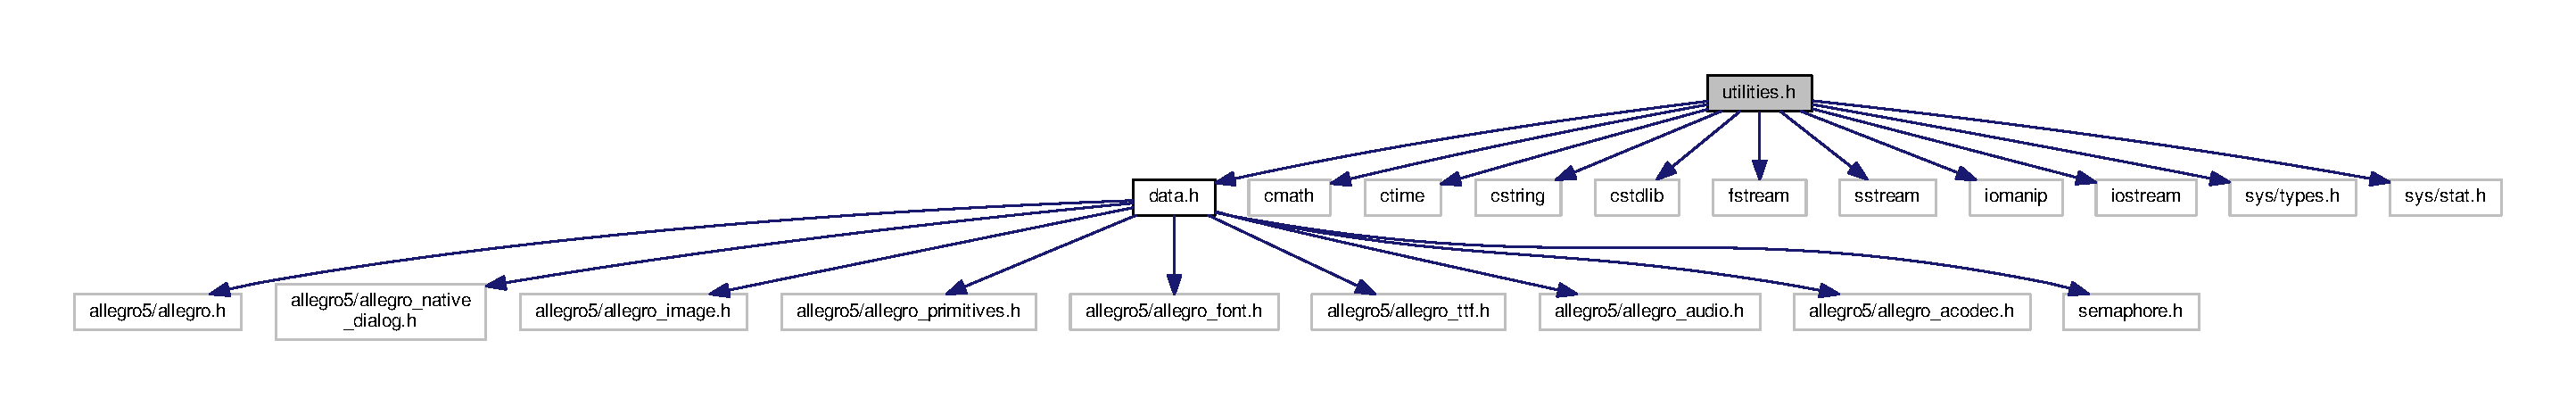
\includegraphics[width=350pt]{de/dfc/utilities_8h__incl}
\end{center}
\end{figure}
Questo grafo mostra quali altri file includono direttamente o indirettamente questo file\+:\nopagebreak
\begin{figure}[H]
\begin{center}
\leavevmode
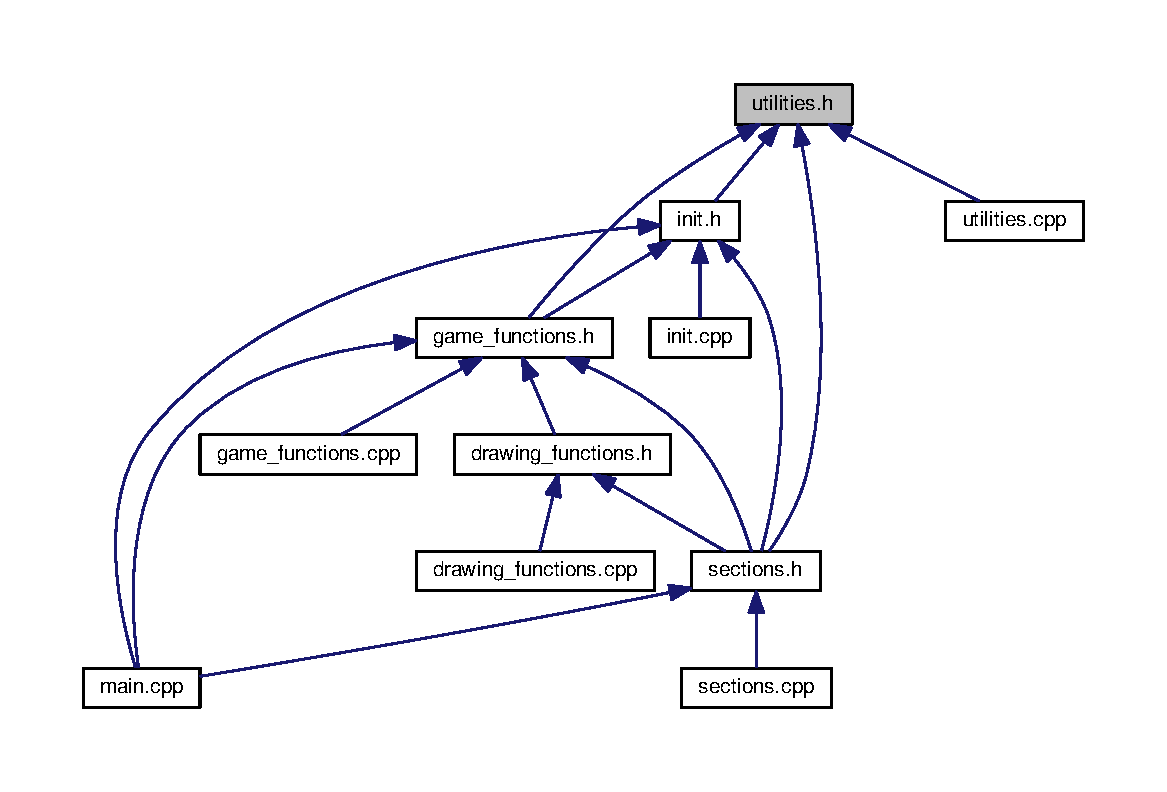
\includegraphics[width=350pt]{d0/db7/utilities_8h__dep__incl}
\end{center}
\end{figure}
\subsection*{Funzioni}
\begin{DoxyCompactItemize}
\item 
bool \hyperlink{utilities_8h_a08c469e6eee9ca9956ac35d64d2124ef}{exit} (A\+L\+L\+E\+G\+R\+O\+\_\+\+D\+I\+S\+P\+L\+AY $\ast$display, const bool playing)
\begin{DoxyCompactList}\small\item\em Funzione ausiliaria che genera un alert con la richiesta di uscire dal gioco. \end{DoxyCompactList}\item 
char $\ast$ \hyperlink{utilities_8h_a09cadb87c7167c969102c415ad70842d}{int\+\_\+to\+\_\+str\+\_\+score} (const int \&match\+\_\+score)
\begin{DoxyCompactList}\small\item\em Funzione che converte il punteggio (intero) in una stringa di otto caratteri. \end{DoxyCompactList}\item 
int \hyperlink{utilities_8h_a9ec487f04fb6ccf162c3fc8f0e672780}{which\+\_\+quadrant} (const float x, const float y)
\begin{DoxyCompactList}\small\item\em Funzione che, dato un certo punto del display, restituisce il quadrante (1-\/4) al quale appartiene. \end{DoxyCompactList}\item 
void \hyperlink{utilities_8h_aeee1998bab6461ac3281a2fd7522a8b9}{extract\+\_\+elem} (\hyperlink{data_8h_a452eef9acfcf76fb85e2c7ecf3b9ff90}{asteroid\+\_\+list} $\ast$ast\+\_\+queues, const int \&index\+\_\+to\+\_\+extract)
\begin{DoxyCompactList}\small\item\em Funzione che estrai l\textquotesingle{}elemento dalla coda. \end{DoxyCompactList}\item 
int \hyperlink{utilities_8h_a045d229cb85f3dbc0d99a421cdcf2a3f}{insert\+\_\+elem\+\_\+head} (\hyperlink{data_8h_a452eef9acfcf76fb85e2c7ecf3b9ff90}{asteroid\+\_\+list} $\ast$ast\+\_\+queues, const \hyperlink{structasteroid__t}{asteroid\+\_\+t} \&asteroid)
\begin{DoxyCompactList}\small\item\em Funzione che inserisce un elemento nella lista, con un controllo se l\textquotesingle{}elemento è inserito in testa o in coda. \end{DoxyCompactList}\item 
void \hyperlink{utilities_8h_a5185c06c8740c026fa53f18b87385767}{change\+\_\+enable} (\hyperlink{data_8h_a56839c56ca6deb3cff5e21540ddb8218}{enable\+\_\+t} \&enable)
\begin{DoxyCompactList}\small\item\em Funzione adibita al set/reset di una determinata impostazione di gioco. \end{DoxyCompactList}\item 
void \hyperlink{utilities_8h_adcafafb6c87ae3399e1d4889a5d5dcce}{delete\+\_\+ast\+\_\+queues} (\hyperlink{data_8h_a452eef9acfcf76fb85e2c7ecf3b9ff90}{asteroid\+\_\+list} $\ast$ast\+\_\+queues)
\begin{DoxyCompactList}\small\item\em Funzione che dealloca gli asteroidi in gioco a fine partita e le relativi immagini. \end{DoxyCompactList}\item 
void \hyperlink{utilities_8h_a68fad52f9f7a53fa048bafc47528a1bb}{delete\+\_\+timer} (\hyperlink{structmatch__vars__t}{match\+\_\+vars\+\_\+t} \&match\+\_\+vars)
\begin{DoxyCompactList}\small\item\em Funzione che dealloca i timer utilizzati come appoggio durante la partita. \end{DoxyCompactList}\item 
void \hyperlink{utilities_8h_a1f78e2ccd2b9605cd499c1d5c7fd62ec}{delete\+\_\+display\+\_\+evqueue\+\_\+music} (A\+L\+L\+E\+G\+R\+O\+\_\+\+D\+I\+S\+P\+L\+AY $\ast$display, A\+L\+L\+E\+G\+R\+O\+\_\+\+E\+V\+E\+N\+T\+\_\+\+Q\+U\+E\+UE $\ast$ev\+\_\+queue, A\+L\+L\+E\+G\+R\+O\+\_\+\+S\+A\+M\+P\+LE $\ast$sound)
\begin{DoxyCompactList}\small\item\em Funzione che dealloca il display, la coda degli eventi e la musica alla chiusera del gioco. \end{DoxyCompactList}\item 
void \hyperlink{utilities_8h_ab1ffd16a1c007a9d9029fc4eaea4abdb}{delete\+\_\+sounds} (\hyperlink{structmatch__vars__t}{match\+\_\+vars\+\_\+t} \&match\+\_\+vars)
\begin{DoxyCompactList}\small\item\em Funzione che dealloca i suoni durante la singola partita. \end{DoxyCompactList}\item 
bool \hyperlink{utilities_8h_a3e3556f55af2c53b4b2790b2e9130b27}{ls\+\_\+tar} (\hyperlink{structls__t}{ls\+\_\+t} $\ast$ls)
\begin{DoxyCompactList}\small\item\em Funzione che restituisce la lista di archivi presenti nella cartella. \end{DoxyCompactList}\item 
bool \hyperlink{utilities_8h_aa56ac46388226ecf231b9da96c5d9084}{archives\+\_\+exist} ()
\begin{DoxyCompactList}\small\item\em Funzione true nel caso la cartella indicata durante la compilazione del programma contenga archivi validi. \end{DoxyCompactList}\end{DoxyCompactItemize}
\subsection*{Variabili}
\begin{DoxyCompactItemize}
\item 
\hyperlink{structdisplay__info__t}{display\+\_\+info\+\_\+t} \hyperlink{utilities_8h_a781a8df874545e4f5bff5f8a446d1963}{display\+\_\+info}
\end{DoxyCompactItemize}


\subsection{Documentazione delle funzioni}
\mbox{\Hypertarget{utilities_8h_aa56ac46388226ecf231b9da96c5d9084}\label{utilities_8h_aa56ac46388226ecf231b9da96c5d9084}} 
\index{utilities.\+h@{utilities.\+h}!archives\+\_\+exist@{archives\+\_\+exist}}
\index{archives\+\_\+exist@{archives\+\_\+exist}!utilities.\+h@{utilities.\+h}}
\subsubsection{\texorpdfstring{archives\+\_\+exist()}{archives\_exist()}}
{\footnotesize\ttfamily bool archives\+\_\+exist (\begin{DoxyParamCaption}{ }\end{DoxyParamCaption})}



Funzione true nel caso la cartella indicata durante la compilazione del programma contenga archivi validi. 

~\newline
Ritorna false altrimenti. \mbox{\Hypertarget{utilities_8h_a5185c06c8740c026fa53f18b87385767}\label{utilities_8h_a5185c06c8740c026fa53f18b87385767}} 
\index{utilities.\+h@{utilities.\+h}!change\+\_\+enable@{change\+\_\+enable}}
\index{change\+\_\+enable@{change\+\_\+enable}!utilities.\+h@{utilities.\+h}}
\subsubsection{\texorpdfstring{change\+\_\+enable()}{change\_enable()}}
{\footnotesize\ttfamily void change\+\_\+enable (\begin{DoxyParamCaption}\item[{\hyperlink{data_8h_a56839c56ca6deb3cff5e21540ddb8218}{enable\+\_\+t} \&}]{enable }\end{DoxyParamCaption})}



Funzione adibita al set/reset di una determinata impostazione di gioco. 

~\newline
Parametri\+: ~\newline
1) enable -\/ Impostazione corrente. \mbox{\Hypertarget{utilities_8h_adcafafb6c87ae3399e1d4889a5d5dcce}\label{utilities_8h_adcafafb6c87ae3399e1d4889a5d5dcce}} 
\index{utilities.\+h@{utilities.\+h}!delete\+\_\+ast\+\_\+queues@{delete\+\_\+ast\+\_\+queues}}
\index{delete\+\_\+ast\+\_\+queues@{delete\+\_\+ast\+\_\+queues}!utilities.\+h@{utilities.\+h}}
\subsubsection{\texorpdfstring{delete\+\_\+ast\+\_\+queues()}{delete\_ast\_queues()}}
{\footnotesize\ttfamily void delete\+\_\+ast\+\_\+queues (\begin{DoxyParamCaption}\item[{\hyperlink{data_8h_a452eef9acfcf76fb85e2c7ecf3b9ff90}{asteroid\+\_\+list} $\ast$}]{ast\+\_\+queues }\end{DoxyParamCaption})}



Funzione che dealloca gli asteroidi in gioco a fine partita e le relativi immagini. 

~\newline
Parametri\+: ~\newline
1) ast\+\_\+queues -\/ Vettore di liste di asteroidi. \mbox{\Hypertarget{utilities_8h_a1f78e2ccd2b9605cd499c1d5c7fd62ec}\label{utilities_8h_a1f78e2ccd2b9605cd499c1d5c7fd62ec}} 
\index{utilities.\+h@{utilities.\+h}!delete\+\_\+display\+\_\+evqueue\+\_\+music@{delete\+\_\+display\+\_\+evqueue\+\_\+music}}
\index{delete\+\_\+display\+\_\+evqueue\+\_\+music@{delete\+\_\+display\+\_\+evqueue\+\_\+music}!utilities.\+h@{utilities.\+h}}
\subsubsection{\texorpdfstring{delete\+\_\+display\+\_\+evqueue\+\_\+music()}{delete\_display\_evqueue\_music()}}
{\footnotesize\ttfamily void delete\+\_\+display\+\_\+evqueue\+\_\+music (\begin{DoxyParamCaption}\item[{A\+L\+L\+E\+G\+R\+O\+\_\+\+D\+I\+S\+P\+L\+AY $\ast$}]{display,  }\item[{A\+L\+L\+E\+G\+R\+O\+\_\+\+E\+V\+E\+N\+T\+\_\+\+Q\+U\+E\+UE $\ast$}]{ev\+\_\+queue,  }\item[{A\+L\+L\+E\+G\+R\+O\+\_\+\+S\+A\+M\+P\+LE $\ast$}]{sound }\end{DoxyParamCaption})}



Funzione che dealloca il display, la coda degli eventi e la musica alla chiusera del gioco. 

Parametri\+: ~\newline
1) display -\/ Puntatore al display del gioco; ~\newline
2) ev\+\_\+queue -\/ Puntatore alla coda di eventi; ~\newline
3) sound -\/ Puntatore alla musica del gioco. \mbox{\Hypertarget{utilities_8h_ab1ffd16a1c007a9d9029fc4eaea4abdb}\label{utilities_8h_ab1ffd16a1c007a9d9029fc4eaea4abdb}} 
\index{utilities.\+h@{utilities.\+h}!delete\+\_\+sounds@{delete\+\_\+sounds}}
\index{delete\+\_\+sounds@{delete\+\_\+sounds}!utilities.\+h@{utilities.\+h}}
\subsubsection{\texorpdfstring{delete\+\_\+sounds()}{delete\_sounds()}}
{\footnotesize\ttfamily void delete\+\_\+sounds (\begin{DoxyParamCaption}\item[{\hyperlink{structmatch__vars__t}{match\+\_\+vars\+\_\+t} \&}]{match\+\_\+vars }\end{DoxyParamCaption})}



Funzione che dealloca i suoni durante la singola partita. 

~\newline
Parametri\+: ~\newline
1) match\+\_\+vars -\/ Contenitore dei puntatori agli audio. \mbox{\Hypertarget{utilities_8h_a68fad52f9f7a53fa048bafc47528a1bb}\label{utilities_8h_a68fad52f9f7a53fa048bafc47528a1bb}} 
\index{utilities.\+h@{utilities.\+h}!delete\+\_\+timer@{delete\+\_\+timer}}
\index{delete\+\_\+timer@{delete\+\_\+timer}!utilities.\+h@{utilities.\+h}}
\subsubsection{\texorpdfstring{delete\+\_\+timer()}{delete\_timer()}}
{\footnotesize\ttfamily void delete\+\_\+timer (\begin{DoxyParamCaption}\item[{\hyperlink{structmatch__vars__t}{match\+\_\+vars\+\_\+t} \&}]{match\+\_\+vars }\end{DoxyParamCaption})}



Funzione che dealloca i timer utilizzati come appoggio durante la partita. 

~\newline
Parametri\+: ~\newline
1) match\+\_\+vars -\/ Contenitore dei puntatori ai tre timer. \mbox{\Hypertarget{utilities_8h_a08c469e6eee9ca9956ac35d64d2124ef}\label{utilities_8h_a08c469e6eee9ca9956ac35d64d2124ef}} 
\index{utilities.\+h@{utilities.\+h}!exit@{exit}}
\index{exit@{exit}!utilities.\+h@{utilities.\+h}}
\subsubsection{\texorpdfstring{exit()}{exit()}}
{\footnotesize\ttfamily bool exit (\begin{DoxyParamCaption}\item[{A\+L\+L\+E\+G\+R\+O\+\_\+\+D\+I\+S\+P\+L\+AY $\ast$}]{display,  }\item[{const bool}]{playing }\end{DoxyParamCaption})}



Funzione ausiliaria che genera un alert con la richiesta di uscire dal gioco. 

~\newline
Parametri\+: ~\newline
1) display -\/ Puntatore al display del gioco; ~\newline
2) playing -\/ Flag per indicare se si sta giocando, in modo da modificare il messaggio; ~\newline
Ritorna un booleano, e indica se si desidera uscire (true) o continuare a giocare (false). \mbox{\Hypertarget{utilities_8h_aeee1998bab6461ac3281a2fd7522a8b9}\label{utilities_8h_aeee1998bab6461ac3281a2fd7522a8b9}} 
\index{utilities.\+h@{utilities.\+h}!extract\+\_\+elem@{extract\+\_\+elem}}
\index{extract\+\_\+elem@{extract\+\_\+elem}!utilities.\+h@{utilities.\+h}}
\subsubsection{\texorpdfstring{extract\+\_\+elem()}{extract\_elem()}}
{\footnotesize\ttfamily void extract\+\_\+elem (\begin{DoxyParamCaption}\item[{\hyperlink{data_8h_a452eef9acfcf76fb85e2c7ecf3b9ff90}{asteroid\+\_\+list} $\ast$}]{ast\+\_\+queues,  }\item[{const int \&}]{index\+\_\+to\+\_\+extract }\end{DoxyParamCaption})}



Funzione che estrai l\textquotesingle{}elemento dalla coda. 

Non sono necessari controlli prima dell\textquotesingle{}estrazione, perchè sono fatti prima della chiamata a questa funzione. ~\newline
Parametri\+: ~\newline
1) ast\+\_\+queues -\/ Vettore di liste di asteroidi; ~\newline
2) character -\/ Iniziale dell\textquotesingle{}elemento da eliminare, cioè indice dell\textquotesingle{}array. \mbox{\Hypertarget{utilities_8h_a045d229cb85f3dbc0d99a421cdcf2a3f}\label{utilities_8h_a045d229cb85f3dbc0d99a421cdcf2a3f}} 
\index{utilities.\+h@{utilities.\+h}!insert\+\_\+elem\+\_\+head@{insert\+\_\+elem\+\_\+head}}
\index{insert\+\_\+elem\+\_\+head@{insert\+\_\+elem\+\_\+head}!utilities.\+h@{utilities.\+h}}
\subsubsection{\texorpdfstring{insert\+\_\+elem\+\_\+head()}{insert\_elem\_head()}}
{\footnotesize\ttfamily int insert\+\_\+elem\+\_\+head (\begin{DoxyParamCaption}\item[{\hyperlink{data_8h_a452eef9acfcf76fb85e2c7ecf3b9ff90}{asteroid\+\_\+list} $\ast$}]{ast\+\_\+queues,  }\item[{const \hyperlink{structasteroid__t}{asteroid\+\_\+t} \&}]{asteroid }\end{DoxyParamCaption})}



Funzione che inserisce un elemento nella lista, con un controllo se l\textquotesingle{}elemento è inserito in testa o in coda. 

Ricavo l\textquotesingle{}indice della coda direttamente da asteroid.\+word\mbox{[}0\mbox{]}. ~\newline
Parametri\+: ~\newline
1) ast\+\_\+queues -\/ Vettore di liste di asteroidi; ~\newline
2) asteroid -\/ Asteroide da inserire. Ritorna un intero, -\/1 se l\textquotesingle{}asteroide è stato inserito in testa altrimenti un indice che rappresenta il numero della coda. \mbox{\Hypertarget{utilities_8h_a09cadb87c7167c969102c415ad70842d}\label{utilities_8h_a09cadb87c7167c969102c415ad70842d}} 
\index{utilities.\+h@{utilities.\+h}!int\+\_\+to\+\_\+str\+\_\+score@{int\+\_\+to\+\_\+str\+\_\+score}}
\index{int\+\_\+to\+\_\+str\+\_\+score@{int\+\_\+to\+\_\+str\+\_\+score}!utilities.\+h@{utilities.\+h}}
\subsubsection{\texorpdfstring{int\+\_\+to\+\_\+str\+\_\+score()}{int\_to\_str\_score()}}
{\footnotesize\ttfamily char$\ast$ int\+\_\+to\+\_\+str\+\_\+score (\begin{DoxyParamCaption}\item[{const int \&}]{match\+\_\+score }\end{DoxyParamCaption})}



Funzione che converte il punteggio (intero) in una stringa di otto caratteri. 

~\newline
Parametri\+:~\newline
1) match\+\_\+score -\/ Il punteggio intero.~\newline
Ritorna il puntatore contenente la stringa formattata. \mbox{\Hypertarget{utilities_8h_a3e3556f55af2c53b4b2790b2e9130b27}\label{utilities_8h_a3e3556f55af2c53b4b2790b2e9130b27}} 
\index{utilities.\+h@{utilities.\+h}!ls\+\_\+tar@{ls\+\_\+tar}}
\index{ls\+\_\+tar@{ls\+\_\+tar}!utilities.\+h@{utilities.\+h}}
\subsubsection{\texorpdfstring{ls\+\_\+tar()}{ls\_tar()}}
{\footnotesize\ttfamily bool ls\+\_\+tar (\begin{DoxyParamCaption}\item[{\hyperlink{structls__t}{ls\+\_\+t} $\ast$}]{ls }\end{DoxyParamCaption})}



Funzione che restituisce la lista di archivi presenti nella cartella. 

~\newline
Parametri\+:~\newline
1) ls -\/ struttura che rappresenta i file contenuti nella cartella. Ritorno false in caso di errore, true altrimenti. \mbox{\Hypertarget{utilities_8h_a9ec487f04fb6ccf162c3fc8f0e672780}\label{utilities_8h_a9ec487f04fb6ccf162c3fc8f0e672780}} 
\index{utilities.\+h@{utilities.\+h}!which\+\_\+quadrant@{which\+\_\+quadrant}}
\index{which\+\_\+quadrant@{which\+\_\+quadrant}!utilities.\+h@{utilities.\+h}}
\subsubsection{\texorpdfstring{which\+\_\+quadrant()}{which\_quadrant()}}
{\footnotesize\ttfamily int which\+\_\+quadrant (\begin{DoxyParamCaption}\item[{const float}]{x,  }\item[{const float}]{y }\end{DoxyParamCaption})}



Funzione che, dato un certo punto del display, restituisce il quadrante (1-\/4) al quale appartiene. 

~\newline
Parametri\+: ~\newline
1) x -\/ Ascissa punto; ~\newline
2) y -\/ Ordinata punto. 

\subsection{Documentazione delle variabili}
\mbox{\Hypertarget{utilities_8h_a781a8df874545e4f5bff5f8a446d1963}\label{utilities_8h_a781a8df874545e4f5bff5f8a446d1963}} 
\index{utilities.\+h@{utilities.\+h}!display\+\_\+info@{display\+\_\+info}}
\index{display\+\_\+info@{display\+\_\+info}!utilities.\+h@{utilities.\+h}}
\subsubsection{\texorpdfstring{display\+\_\+info}{display\_info}}
{\footnotesize\ttfamily \hyperlink{structdisplay__info__t}{display\+\_\+info\+\_\+t} display\+\_\+info}


%--- End generated contents ---

% Index
\backmatter
\newpage
\phantomsection
\clearemptydoublepage
\addcontentsline{toc}{chapter}{Indice}
\printindex

\end{document}
